\documentclass{report}

\usepackage[utf8]{inputenc}
\usepackage{titlesec}
\usepackage{easylist}
\usepackage{hanging}
\usepackage{hyperref}
\usepackage[a4paper,top=2.5cm,bottom=1.8cm,left=2.5cm,right=2.5cm]{geometry}
\usepackage{blindtext}
\usepackage{tipa}
\usepackage{epigraph}
\usepackage{enumerate}
\usepackage{longtable}
\usepackage{setspace}
\usepackage{verbatim}
\usepackage[T1]{fontenc}
\usepackage{graphicx}
\usepackage[italian]{babel}
\usepackage{amsmath}
\usepackage{pbox}
\usepackage{fancyhdr}
\usepackage{cancel}
\usepackage{tabularx}
\usepackage{booktabs}
\usepackage{multirow}
\usepackage{longtable}
\usepackage{tikz}
\usepackage{tikz-qtree}
\usepackage{subfig}
\usepackage[rgb]{xcolor}
\usepackage{amssymb}
\usepackage{mathrsfs}
\usepackage{textcomp}
\usepackage{verbatim}

% algoritmi pseudo
\usepackage[]{algorithm2e}

\usepackage{pgfplots}

\usepackage{listings}
\usepackage{color}

\definecolor{mygreen}{rgb}{0,0.6,0}
\definecolor{mygray}{rgb}{0.5,0.5,0.5}
\definecolor{mymauve}{rgb}{0.58,0,0.82}

\lstset{ 
  backgroundcolor=\color{white},   % choose the background color; you must add \usepackage{color} or \usepackage{xcolor}; should come as last argument
  basicstyle=\footnotesize,        % the size of the fonts that are used for the code
  breakatwhitespace=false,         % sets if automatic breaks should only happen at whitespace
  breaklines=true,                 % sets automatic line breaking
  captionpos=b,                    % sets the caption-position to bottom
  commentstyle=\color{mygreen},    % comment style
  deletekeywords={...},            % if you want to delete keywords from the given language
  escapeinside={\%*}{*)},          % if you want to add LaTeX within your code
  extendedchars=true,              % lets you use non-ASCII characters; for 8-bits encodings only, does not work with UTF-8
  firstnumber=1000,                % start line enumeration with line 1000
  frame=single,	                   % adds a frame around the code
  keepspaces=true,                 % keeps spaces in text, useful for keeping indentation of code (possibly needs columns=flexible)
  keywordstyle=\color{blue},       % keyword style
  language=Octave,                 % the language of the code
  morekeywords={*,...},            % if you want to add more keywords to the set
  numbers=left,                    % where to put the line-numbers; possible values are (none, left, right)
  numbersep=5pt,                   % how far the line-numbers are from the code
  numberstyle=\tiny\color{mygray}, % the style that is used for the line-numbers
  rulecolor=\color{black},         % if not set, the frame-color may be changed on line-breaks within not-black text (e.g. comments (green here))
  showspaces=false,                % show spaces everywhere adding particular underscores; it overrides 'showstringspaces'
  showstringspaces=false,          % underline spaces within strings only
  showtabs=false,                  % show tabs within strings adding particular underscores
  stepnumber=2,                    % the step between two line-numbers. If it's 1, each line will be numbered
  stringstyle=\color{mymauve},     % string literal style
  tabsize=2,	                   % sets default tabsize to 2 spaces
  title=\lstname                   % show the filename of files included with \lstinputlisting; also try caption instead of title
}

\linespread{1.2} % l'interlinea

\frenchspacing

\newcommand{\abs}[1]{\lvert#1\rvert}

\usepackage{floatflt,epsfig}

\usepackage{multicol}
\newcommand\yellowbigsqcup[1][\displaystyle]{%
  \fboxrule0pt
  \ifx#1\textstyle\fboxsep-0.6pt\else\fboxsep-1.25pt\fi
  \mathrel{\fcolorbox{white}{yellow}{$#1\bigsqcup$}}}

\newtheorem{nota}{Nota}[section]
\newtheorem{descrizione}{Descrizione}[section]
\newtheorem{notab}{Nota bene}[section]
\newtheorem{esempio}{Esempio}[section]
\newtheorem{defi}{Definizione}[section]

\title{Laboratory of image processing for computer vision}
\author{Nicola Ferru}
\begin{document}
\maketitle
\tableofcontents
\chapter{Introduzione}
\label{chap:intro}
\section{Sommario}
Qui di seguito sono riportati i concetti fondamentali trattati all'interno del documento
\subsection{Informazione e segnali}
\label{sec:Informazioneesegnali}
L'informazione sussiste solo se il ricevente della trasmissione non conosce il
contenuto della suddetta.\\ Per esistere una trasmissione devono esserci:
\begin{enumerate}
  \item Comunicazione;
  \item Mezzo di trasmissione;
  \item Informazione.
\end{enumerate}

\subsection{Informazioni analogiche e digitali}
\label{sec:andiginfo}
Visto che è un argomento riccorrente all'interno del programma è giusto dare quanto
meno, una definizione anche se stringata, quindi:
\begin{defi}
  \label{def:andef}
  si dicono grandezze analogiche quelle che possono assumere tutti i valori
  intermedi all'interno di un dato intervallo; Si dicono grandezze digitali
  quelle che vengono espresse in modo numerico, senza possibilità di
  discriminare valori intermedi tra due cifre consecutive.
  Ulteriori approfondimenti presenti in (\ref{sec:sanalog})
  \footnote{\href{https://it.wikipedia.org/wiki/Analogico}{https://it.wikipedia.org/wiki/Analogico}}
\end{defi}
\begin{defi}
  \label{def:digdef}
  Con digitale o numerico, in informatica ed elettronica, ci si riferisce a tutto ciò che
  viene rappresentato con numeri o che opera manipolando numeri, contrapposto all'analogico. Ulteriori approfondimenti presenti in (\ref{sec:sdigital})
  \footnote{\href{https://it.wikipedia.org/wiki/Digitale_(informatica)}{https://it.wikipedia.org/wiki/Digitale\_(informatica)}}
\end{defi}
\begin{oss}
  \label{oss:strumMisura}
  Tipicamente quando si tratta di strumenti di misurazione entrambi i tipi di
  informazione entrano in gioco per poter funzionare. Ad esempio una sonda per
  un formo prende in ingresso in informazione analogica ``la temperature'' e poi
  la converte tramite l'apposito ADC a un informazione digitale per poterla
  campianare ed elaborare tarmite una centralina di gestione. 
\end{oss}
Oggi ormai utilizziamo il digitale perché effettivamente i calcolatori
elettronici gestiscono meglio una codifica rispetto a dei numeri reali. Per di
più costa meno produrre un dispositivo che gestisca segnali digitali rispetto
ad un dispositivo che gestisce mezzi analogici.
Ad esempio la differenza tra lo standard VHS e lo standard CD/DVD/Blue Ray, infatti,
il VHS era uno standard basato su un nastro magnetico, cosa che negli ultimi suoi anni
di vita si mescolò anche con il digitale ma uno dei limiti veri restava proprio il
supporto fisico, infatti, il nastro magnetico è molto fragile e incline ad avere
tantissimi problemi anche di prestazioni in utilizzi di archiviazione dati.
\subsection{Alcune osservazioni}
\begin{itemize}
\item Non tutte le informazioni costituiscono un vero e proprio contenuto
  inforamtivo
  \begin{enumerate}
  \item La notizia comunicata deve per noi essere eclatante;
  \item una persona noiosa non apporta informazione perché ripete
    continuamente gli stessi argomenti.
  \end{enumerate}
\item Problema di misurazione del contenuto informativo
  \begin{itemize}
  \item {\bf Claude E. Shannon} ({\tt 1916-2001}), fondatore della
    \textit{Teoria Matematica dell'Informazione}, è stato il primo
    ad introdurre la distinzione tra forma e significato nel
    processo comunicativo.
  \end{itemize}
\end{itemize}
\subsubsection{I risultati di Shannon}
\begin{itemize}
	\item Non è possibile definire la quantità di informazione associata ad un
		messaggio già ricevuto, ma piuttosto la quantità di informazione
		associata ad un papabile messaggio
		\begin{itemize}
			\item \textit{``information is that which reduces uncertainty''}
		\end{itemize}
	\item La quantità di informazione associata ad un massaggio è tanto più
		altra quanto più esso è inatteso
		\begin{itemize}
			\item il messaggio ``{\bf domani sorgerà il sole}'' ha un bassissimo
				contenuto informativo perché è assolutamente scontato e banale
			\item il messaggio ``{\bf Domani scoppierà la guerra}'' ha un alto
				contenuto informativo.
		\end{itemize}
\end{itemize}
\section{I segnali}
\begin{itemize}
	\item \textit{Grandezze fisiche variabili nel tempo a cui è associata
		un'informazione};
	\item \textit{L'informazione è associata ad una variazione ({\color{red}
		aleatorio} e non deterministica) della grandezza fisica};
	\item Aleatorio (dal latino ``alea'', gioco di dati) è sinonimo di non
		predicibile a priori (in contrapposizione con deterministico).
\end{itemize}
\subsection{Rappresentazione dell'informazione}
\label{sec:rappredellinfo}
\begin{itemize}
\item Associazione tra caratteristiche (di valore e temporali) dei segnali
  e le informazioni che essi rappresentano;
\item Le caratteristiche sono impresse dal dispositivo generatore del
  segnale;
\item Quali caratteristiche?
  \begin{itemize}
  \item valore, andamento temporale ed eventi del segnale (es.
    superare una soglia), etc.
  \end{itemize}
\end{itemize}
\subsection{Classificazione di segnali}
\label{sec:classsegn}
I segnali vengono classificati in base alla loro natura e alle loro caratteristiche.
Tipicamente per il campionamento avviene il seguente processo:
\begin{center}
  Grandezza fisica \textrightarrow{} trasduttore \textrightarrow{} segnale elettrico 
\end{center}
Quindi prendendo come base questa affermazione, possiamo dire che un segnale che sia
di natura elettrica, acustica o qualunque altra natura fisica, può essere campionato
da uno strumento che tramite il suo trasduttore converdirà in un istruzione
``tipicamente definita pacchetto di istruzioni o di informazioni'' che a sua volta
verrà convertito in un segnale elettrico che seguendo lo standard di comunicazione
del modello\footnote{una variazione della corrente elettrica o di tensione all'interno
  di un conduttore oppure in un punto di un circuito elettrico o elettronico.} di
rifimento potrà essere trasmesso o elaborato da un computer o da una centralina
dedicata a scopo di analisi oppure per inviarlo altrove. Ad esempio, se noi campioniamo
una chitarra elettrica sfruttando un pickup magnetico, il processo sarà il seguente:
\begin{center}
  Vibrazione della corda [\textit{pickup}] \textrightarrow{} scheda audio
  \textrightarrow{} segnale elettrico che il computer può leggere
\end{center}
Ed ecco come associare un caso di quotidiano all'argomento, infatti, la pratica qui
illustrata è un aspetto molto presente nella nostra vita, molti degli oggetti che
circondano la vita dell'individuo seguono questa logica.
\section{Spiegazione sui segnali}
\label{sec:spsegn}
\subsection{Segnali analogici}
\label{sec:sanalog}
\begin{itemize}
\item il valore dell'informazione rappresentata è una funzione continua
  della grandezza significativa;
\item rappresentazione attraverso un numero reale (\textit{con precisione
    teoricamente infinita})
\item generati da sensori o trasduttori che creano una corrispondenza tra
  la grandezza fisica che è oggetto di informazione (\textbf{esempio
    temperatura}) e il segnale (\textbf{esempio tensione elettrica})
\end{itemize}
\subsubsection{Esempi}
\begin{itemize}
	\item \textbf{Temperatura:} altezza in \texttt{mm} del mercurio nel
		termometro;
	\item \textbf{Acustico:} variazione di pressione ad un microfono;
	\item \textbf{Elettrico:} tensione ai capi di un conduttore.
\end{itemize}
\subsection{Segnali digitali}
\label{sec:sdigital}
\begin{itemize}
	\item rappresentazione come sequenza di numeri presi da un insieme di
		valori discreti, ovvero appartenenti a uno stesso insieme ben definito
		e circoscritto;
	\item rappresentazione ``{\bf a fasce}''
\end{itemize}
\begin{oss}
  L'attributo ``analogico'' o ``digitale'' non si riferisce a caratteristiche
  intrinseche del segnale ma a caratteristiche dell'informazione da esso rappresentato:
  {\color{red} I segnali digitali nascono come analogici}
\end{oss}
\subsection{Pregi e difetti}
\label{sec:pregiedifettideisegnali}

\subsubsection{Analogico}
\label{sec:analdifpreg}
\paragraph{Pregi}

\begin{tasks}(2)
	\task Sono più ``naturali'', le leggi della fisica classica operano
	tipicamente nel ``continuo'';
	\task Il rumore deforma ma non stravolge il segnale (errori proporzionali
	all'entità del disturbo ``{\bf in onde media la radio analogica la senti,
	anche se con un forte rumore bianco di fondo.}'')
\end{tasks}
\paragraph{Difetti}
\begin{tasks}(2)
	\task Dispositivi di elaborazione relativamente poco precisi, poco stabili
	nel tempo ``maggiormente predisposti ai guasti, alle intemperie e anche a
	potenziali variazioni atmosferiche'' e poco immuni alle perturbazioni;\\
	({\tt esempio}: il video registratore VHS ``M-matic'' o sony U-matic, sono
	apparecchi estremamente complessi, soprattutto gli ultimi per metà digitali
	con tante funzionalità e tasti programmabili per fasce orarie, perfetti per
	registrale le trasmissioni in modo autonomo.)
	\task Le elaborazioni su di essi sono poco flessibili e producono degrado.
\end{tasks}
\clearpage
\section{Il sistema numerico binario}
\label{sec:sistemanumbin}
\begin{defi}
  il sistema numeri Binario è un sistema di numerazione utilizzato per i calcolatori
  elettronici e sviluppato per soperire a lato prestazionale di calcolo per i
  suddetti\footnote{Un calcolatore elettronico riesce a processare più velocemente
    casi che possono avere poche possibilità, il binario per singola posizione può
    avere solo due possibilità 0 o 1}. Infatti, nel segnale digitale esite il seguente
  caso:
  \begin{itemize}
  \item 1 sta al Vero logico, in gergo ``TRUE'' oppure livello alto, in gergo ``HIGH''.
  \item 0 sta al Falso logico, in gero ``FALSE'' oppure livello basso, in gergo ``LOW''.
  \end{itemize}
  Il vantaggio di questo sistema è che con la logica positiva o negativa, risolve molti
  casi, tra cui il fatto che il singolo termine ``bit'' non sia segnato\footnote{Non è
    positivo o negativo, per avere il corrispettivo decimale con il segno si usa una
    codifica sacrificando un bit per attribuirgli la funzione di segno, se esso è pari a
    0 il numero, mentre, se il bit di segno è pari a 1 il numero è negativo.}, questo
  lo si vedrà nel dettaglio nei dettaglio in (\ref{<-->}) 
\end{defi}

\subsection{La rappresentazione}
\label{sec:rapbin}

La cosa comoda del sistema binario è il fattore di conversione, infatti, questa
codifica permette di rappresentare un qualunque numero decimale senza segno compreso
tra $0$ e $2^n-1$ tramite una sommatoria per posizione, come spressa nella seguente
formula:
\begin{equation}
  \label{eq:rappbin}
  (a_{n-1},\dots,a_1,a_0)_2\to \sum\limits^{n-1}_{i=0} a_i,b^i
\end{equation}
Dove $(a_{n-1})$ è la cifra più significativa e $a_0$ è quella meno significativa.
\begin{equation}
  \label{eq:esempiodiconversione}
  (10101110)_2\Leftrightarrow (174)_{10} \Leftrightarrow (AE)_{16}
\end{equation}

\subsection{Rappresentazione del modulo e del segno}
\label{sec:modesegnoinbin}
Il bit più significativo viene utilizzato per la rappresentazione del segno, mentre
il resto viene utilizzato per il modulo.
\begin{nota}
  questo sistema fa perdere un bit di rappresentazione quindi il valore rappresentato è
  pari al N-1, ad esempio su 8 bit che consentono di rappresentare fino al
  valore $(256)_{10}$ se andiamo ad applicare il bit segnato avremmo 7bit di
  rappresentaione per il modulo e 1bit per il segno cosa che porta la rappresentazione
  possibile al massimo a $(127)_{10}$ e $(-128)_{10}$
\end{nota}
Ma per essere più specifici meglio utilizzare una somma in forma tabellare per mostrare
l'esito dei segni in una somma tra due numeri $A$ e $B$:
\begin{equation}
  \label{eq:sommabin1}
  \begin{matrix}
    & \text{Segno di } B\\
    \text{Segno di } A &
                       \begin{array}{|ccc|}
                         &+&-\\
                         +& A+B & A-\abs{B}\\
                         - & B-\abs{A} & \abs{A}+\abs{B}
                       \end{array}
  \end{matrix}
\end{equation}

\subsection{Rappresentazione di complemento a 1}
\label{sec:rappcompa1}
Il bit più significativo rappresenta il segno, come nel caso di qui sopra
\begin{itemize}
\item stesso intervallo di valore rappresentabili con modulo e segno.
\end{itemize}
Un numero negativo si ottiene dal positivo cambiando tutti i bit:
\begin{itemize}
\item Il numero 6 in binario si scrivi 0110 prendeno un caso a 4 bit segnati ma
  se noi vediamo come si scrive il -6 il risultato è il seguente 1001 l'esatto inverso
  del numero positivo.
\end{itemize}
nelle operazione aritmetiche si utilizza l'eventuale riporto necessario a compensare
la mancanza di altri simboli al difuori dello 0 e del 1.
\begin{esempio}
  Prediamo una semplice somma come $22+3=25$, in questo caso per rappresentare
  l'operazione in colonna sono stati disposti 8 bit nonostante i numeri non sforino
  i 6.
  \begin{equation}
    \label{eq:compa1}
    \begin{array}{lccr}
      &&{\color{red}1100}&\\
       & 0001 & 0110 & (22)\\
      +& 0000 & 0011 & (3)\\\hline
       & 0001 & 1001 & (25)
    \end{array}
  \end{equation}
  I bit in rosso sono il riporto, infatti in questo caso è bastato solo un complemento a
  1 in cui il riporto non sfora dal numero di bit stimati, in gergo tecnico si tratta
  di un overflow, cosa che se avviene all'interno di un programma sul proprio computer
  può causare dei problemi, che siano di memoria perché satura la ram, potrebbe
  compromettere un altro processo se va a scrivere in un aria di memoria non adibito
  al suddetto processo oppure semplicemente se è un calcolo esso verrà tagliato e
  quindi barliamo di perdita di informazione.
\end{esempio}
\subsection{Rappresentazione di complemento a 2}
\label{sec:rappcompa2}
Il complemento a 2 è molto similare al complemento a 1 visto nel capitolo
(\ref{sec:rappcompa1}) con due sostaziali differenze -- La prima è un vantaggio,
infatti, in questo caso esiste un unica rappresentazione per lo zero, mentre,
la seconda è il fatto che si ignora l'overflow visto che i riporti molte volte
supereranno il valore rappresentabile.
\begin{esempio}
  Prendendo una semplice somma $31-5=26$, andiamo a fare il complemeto a due sfruttando
  in questo caso gli 8 bit pieni per il riporto, anche in questo caso le basi dei due
  addendi non superano i 6 bit ma per una questione di convenzione ``si usano basi
  multipli di 2, quindi il numero di bit devono essere 4, 8, 16, 32, 64, etc\dots''
  \begin{equation}
    \label{eq:compa2}
    \begin{array}{lccr}
      &{\color{red}1111}&{\color{red}1110}\\
      &0001&1111&(31)\\
      +&0000&1011&(-5)\\\hline
      &0001&1010&(26)
    \end{array}
  \end{equation}
  La differenza tra l'operazione (\ref{eq:compa1}) e la (\ref{eq:compa2}) sono poche
  ma significative, come si vede, i bit di riporto arrivano fino a sforare gli 8 bit
  nonostante ciò il risultato si ferma giustamente al quinto bit che im qiest caso
  è il più significativo e l'effetto del riporto sull'uno nella quarta posizione a
  partire da sinistra resta immutato proprio in virtù di quel principio.
\end{esempio} 
\subsection{Confronto}
\label{sec:controntotracomplementi}

\begin{table}[h!]
	\centering
	\begin{tabular}{|c|c|c|c|c|c|c|}
		\hline
		\multirow{2}{*}{Stringa}&\multicolumn{4}{c|}{rappresentazione}\\
		&senza segno&modulo e segno&complemento a 1&complemento a 2\\\hline
		000&0&0&0&0\\\hline
		001&1&1&1&1\\\hline
		010&2&2&2&2\\\hline
		011&3&3&3&3\\\hline
		100&4&0&-3&-4\\\hline
		101&5&-1&-2&-3\\\hline
		110&6&-2&-1&-2\\\hline
		111&7&-3&0&-1\\\hline
	\end{tabular}
	\caption {Confronto tra il modulo e segno, complemento 1 \& 2}
\end{table}

\section{Sistemi di comunicazione}
\label{sec:siscom}
Per poter rendere utile l'informazione è necessario per forza di cose che esistano degli
standard per poter comunicare, dei canali di comunicazione e dei sistemi dedicati alle
comunicazioni, ad esempio un libro consente di acquisire delle informazioni mediante
la scrittura che è codificata con dei caratteri in una determinata lingua oppure
un esempio ancora più immediato, prendiamo una comunicazione verbale tra due persone,
in quel caso il sistema di comunicazione è composto dai due individue, dall'aria che è
il canale di comunicazione e dalla lingua che è la codifica, se anche solo uno dei punti
non è soddisfatto la comunicazione non è efficace ``se i due individue parlano lingue
diverse non si va da nessuna parte'' non non avviene proprio ``in assenza d'aria non
si può parlare''
\subsection{Trasmissione e recezione}
\label{sec:trasmerec}
Il sistema di comunicazione per essere efficente prevede due elementi; la trasmissione
e la recezione che funzina nel guente modo:

\subsubsection{La trasmissione}
\label{sec:trasm}
Come visto in (\ref{sec:classsegn}) l'acquisizione di una informazione avviene
mediante un trasduttore che consente una conversione in un formato comprensibile
al calcolatore dopo che viene fatto questo processo di trasformazione tramite il
trasduttore sarà anche possibile diffonderlo tramite un canale di comunicazione.
\begin{center}
  Sorgente fisica \textrightarrow{} Trasduttore \textrightarrow{} TX \textrightarrow{}
  Al canale di comunicazione
\end{center}
Come chiaro dai passaggi, il TX ``dispositivo adito alla trasmissione'' è posto dopo
il trasduttore per motivi puremante essenziali, il messaggio per poter assere inviato
deve essere prima trasformato o per meglio dire tradotto in una codifica che sia chi
sta trasmettendo sia chi poi dovrà ricevere il suddetto messaggio devono conoscere,
altrimenti la comunicazione non riesce. Ovviamente il sengale nel canale di
comunicazione rispetterà criteri analogici e fisici per essere trasmesso, poi del
riportare l'istruzione alla forma leggibile ci penserà ricevitore.
\subsubsection{La recezione}
\label{sec:recezione}
Il processo di recezione è l'esatto opposto di quello di trasmissione, infatti,
presuppone che ci sia uno strumento in ascolto per catturare il segnale emesso,
infatti, il primo step nella catena di recezione è priprio il canale di comunicazione
\begin{center}
  Dal canale di communicazione \textrightarrow{} RX \textrightarrow{} Trasduttore
  \textrightarrow{} Utente finale
\end{center}
In questo caso il RX è il dispositivo in ascolto, poi ci sarà il trasduttore che
trasformera il segnale in un formato leggibile e poi l'utente finale che usufruira
dell'informazione acquisita.
\subsection{Classificazione di sistemi}
\label{sec:classidisistemi}
\begin{table}[ht]
  \centering
  \begin{tabular}{ll}
    \textbf{Punto-Punto} & \textbf{Multi-utente}\\\hline
    1 trasmettitore & 1 o più trasmettitore iniziali\\\hline
    1 o più ripetitori intermedi & 1 o più ripetitori\\\hline
    1 ricevitore & Il canale è una risorsa condivisa tra i diversi\\
                         & trasmettitori e/o ricevitori presenti nel sistema\\\hline
    Ad ogni tratto vengono associati uno o più & broadcast se coinvolge tutti gli utenti\\
    mezzi fisici di propagazione del segnale & come ricevitori.\\\hline
    Il canale è una risorsa dedicata al collegamento\\\hline
  \end{tabular}
  \caption{Classi di sistemi}
  \label{tab:classificazionedisistema}
\end{table}

\subsection{Rete di telecomunicazione}
\label{sec:retetele}

Quando si parla di reti di telecounicazioni si pensa sempre alla piattaforma tecnologica
su cui è basata, gli obbiettivi e le modalità di comunicazione.

\subsubsection{Obbiettivi}
\label{sec:obbiettivireti}
\begin{enumerate}
\item Effetuare comunicazione a distanza tra due o più utenti;
\item Trasferire informazione (servizio di telecomnicazioni) caratterizata diversi
  parametri (durata, qualità, etc.);
\item Gestire le sue parti componenti e i servizi supportati
\end{enumerate}
Ci sono diverse modalità (e dunque topologie) per realizzare tale trasferimento:
vantaggi/svantaggi.
\clearpage
\paragraph{Criteri di classificazione di reti}

La classificazione può essere basata sui seguenti criteri:
\begin{multicols}{2}
  \begin{enumerate}
  \item La gamma del servizi supportati;
  \item Grado di mobilità del terminale;
  \item l'Estensione fisica della rete;
  \item la posizione.
  \end{enumerate}
\end{multicols}

\subsection{Classificazione per servizi}
\label{sec:classperservizi}
Le reti vengono classificate anche per il criterio del servizio, infatti, esistono
reti dedicate, che svolgono solamente quel servizio e le reti integrata nei servizi
che consentono di svolgere più servizi con la stessa rete. Le differenze sono le
seguenti:
\begin{table}[ht]
  \centering
  \begin{tabular}{ll}
    Rete \textbf{Dedicata} ad un servizio & Reti \textbf{integrata nei servizi}\\\hline
    Fornitore di un singolo servizio & Fornitura di una vasta gamma di servizi\\\hline
    Possono essere utilizzate con alcune & Prestazioni complessive di qualità e di costo\\
    limitazioni anche per un insieme & decisamente migliori rispetto a quella ottenibile\\
    ristretto di altri servizi. & con le reti dedicate.\\\hline

    L'esempio: la rete telefonica fissa & L'esempio: Internet e le reti mobile della\\
    generazioni di reti mobili ({\it GSM}) & generazione 2G in poi.\\\hline
  \end{tabular}
  \caption{Classificazione per servizi}
  \label{tab:classperserv}
\end{table}
\begin{oss}
  Al giorno d'oggi è più diffusa la seconda categoria di rete perché costa meno e può
  svolgere più di un servizio e con il fatto che restano solo pochi sistemi anche la
  manutenzione costa meno e si possono investire i fondi per rendere tutto più stabile e
  tollerante ai guasti.
\end{oss}
\subsection{Classificazione per mobilità}
\label{sec:classificazionemobile}
\begin{table}[ht]
  \centering
  \begin{tabular}{ll}
    \texttt{Rete fissa} & \texttt{Rete mobile}\\\hline
    Gli utenti accedono alla rete da postazioni fisse, & gli utenti possono muoversi senza limitazioni\\
    oppure si muovono in un interno relativamente.  & al loro spostamenti (anche tramite veicoli) \\
    ristretto &\\\hline
    Il punto di accesso fisso, terminale può essere mobile & Gli utenti possono cambiare\\
                        & ``punto di accesso'' alla rete che gestisce ciò\\
                        &  rendendoli sempre raggiungibili (handever)\\\hline
    ad esempio terminali Wi-Fi che accedono ad Internet & ad esempio i cellulari\\\hline
  \end{tabular}
  \caption{Classificazione per mobilità}
  \label{tab:classipermobile}
\end{table}
\begin{nota}
  Le reti mobili hanno il vantaggio della portabilità del servizio ma hanno alcuni
  limiti, tra cui la copertura del proprio ISP (\underline{Internet Service Provider})
  e le prestazioni sono inferiori rispetto a quello cablato.
\end{nota}

\subsection{Classificazione per estensione}
\label{sec:classest}
Le reti di telecomunicazioni si suddividono anche per portata massima, questa
nomenclatura viene utilizzata per le reti internet e VoIP, partendo dalla più
piccola per portata la PAN alla più estesa la WAN. 
\begin{table}[ht]
  \centering
  \begin{tabular}{llll}
    PAN& LAN& MAN & WAN\\\hline
    Area personale & Area locale & Area relativamente estesa & Area molto estesa\\
    (circa 1m) & (max pochi km) & (Città, decina di km) & (nazione, centinaia di km)\\
    \hline
    Bluetooth & Ethernet, Wi-Fi & WiMAX & Internet, rete telefonica\\\hline
  \end{tabular}
  \caption{Classificazione per estensione}
  \label{tab:classest}
\end{table}

\subsection{Interconnessione di reti}
\label{sec:interdireti}
Uno dei fondamenti delle telecomunicazione è proprio l'interconnessione cioè la
possibilità di connettere più reti a sieme, infatti, esiste la possibilità di unire
più reti {\tt PAN} in una rete {\tt LAN}.
\begin{center}
  (PAN $\longleftrightarrow$ PAN $\longleftrightarrow$ PAN) LAN
\end{center}
Con questo sistema si ottengono reti di tipo omogeneo e si aggiungono opportuni
meccanismi e protocolli comini operanti sempre le varie reti componenti.

\subsection{Classificazione per posizione}
\label{sec:classperposiz}

Le reti di trasmissione interconnette tra di loro le reti di accesso permettendo le
comumicazioni tra terminali di utenti remoti collegati a differenti reti di accesso.
In riferimento alla rete più grossa di cui fa parte, viene anche chiamata
``Core Network''.
\begin{center}
  \Tree[.Rete\ di\ trasmissione rete\ di\ accesso rete\ di\ accesso rete\ di\ accesso ] 
\end{center}
Nel caso delle reti di accesso interconnette tra di loro i terminali presenti in un'area
limitata e questo con una rete di trasmissione.

\subsection{Soggetti implicati}
\label{sec:soggimp}

\begin{table}[ht]
  \centering
  \begin{tabular}{lll}
    \textbf{Gestore di rete}&\textbf{Fornitore del servizio}&\textbf{Cliente del servizio}\\\hline
    Network operator: attiva e mantiente & Service Provider: rende fruibile & Soggetto della \\
    operativa la piattaforma di rete per & il servizio al cliente secondo & comunicazione (sorgente e/o\\
    assicurare la fruizione dei servizio & modalità (e.g. costo, durata) & destinatario)
  \end{tabular}
  \caption{Soggetti implicati nella gestione del servizio di rete}
  \label{tab:sggimp}
\end{table}

\section{Rami e nodi}
\label{sec:ramienodi}
\begin{defi}
  La rete è un insieme di nodi e di rami quindi nel tempo
  sono nate diverse dopologie per sopperire alle esigenze. Al momento le topologie più
  diffuse sono:
  \begin{itemize}
  \item A maglia;
  \item A Stella o Grafo;
  \item Ad Nello.
  \end{itemize}
  Ne esistono anche delle altre ma non sono altrettanto diffuse. Alcune topologie
  non sono più utilizzate in quanto frutto dei primi esperimenti a riguardo ma non
  efficenti, altre non si sono diffuse per un puro andamento di mercato.
  Tra l'altro le topologie prima citate in un caso reale vengono mescelete per poter
  ottenere una maggiore tolleranza ai guasti. 
\end{defi}
\begin{figure}[ht]
  \centering
  \resizebox{10cm}{!}{\def\a{.4}
\def\b{.3}
\def\cr{.53}

\begin{tikzpicture}
% bus topograpy
\draw (2,-1) circle (\a cm);
\draw (2,-1) -- (2,0);
\draw (4,-1) circle (\a cm);
\draw (4,-1) -- (4,0);
\draw (1,1) circle (\a cm);
\draw (1,1) -- (1,0);
\draw (3,1) circle (\a cm);
\draw (3,1) -- (3,0);
\draw (5,1) circle (\a cm);
\draw (5,1) -- (5,0);
\draw (0,0) -- (6,0);

% star topograpy
\draw (10,0) -- (8.5,-1);
\draw (8.5,-1) circle(\b cm);

\draw (10,0) -- (11.5,-1);
\draw (11.5,-1) circle(\b cm);

% centro
\draw (10,0) circle(\cr cm);

\draw (10,0) -- (10,-1.7);
\draw (10,-1.7) circle(\b cm);

\draw (10,0) -- (9,1);
\draw (9,1) circle(\b cm);

\draw (10,0) -- (11,1);
\draw (11,1) circle(\b cm);

% Rete ad anallo

\draw (13.5,-1) circle(\b cm);
\draw (13.5,-1) -- (14.5,-1.7);
\draw (13.5,-1) -- (14,0.4);

\draw (15.5,-1) circle(\b cm);
\draw (14.5,-1.7) -- (15.5,-1);

\draw (14.5,-1.7) circle(\b cm);
\draw (15.5,-1) -- (15,0.4); 

\draw (14,0.4) circle(\b cm);

\draw (15,0.4) circle(\b cm);
\draw (14,0.4) --  (15,0.4);

% modello a maglia
\draw (17,-1) circle(\b cm);
\draw (19,-1) circle(\b cm);
\draw (17,-1) -- (19,-1);

\draw (17,-1) -- (18,-1.7);
\draw (18,-1.7) circle(\b cm);
\draw (18,-1.7) -- (19,-1);

\draw (18,-1.7) -- (17.4,0.4); 
\draw (17.4,0.4) circle(\b cm);
\draw (17,-1) -- (17.4,0.4);
\draw (17.4,0.4) -- (19,-1);

\draw (18.7,0.4) circle(\b cm);
\draw (18,-1.7) -- (18.7,0.4);
\draw (17,-1) -- (18.7,0.4);
\draw (17.4,0.4) -- (18.7,0.4);
\draw (19,-1) -- (18.7,0.4);
\end{tikzpicture}}
  \caption{Topologie a bus, a stella, ad anello e a maglie}
  \label{fig:topologiepiùutilizzate}
\end{figure}
\begin{oss}
  La topologia a bus era la prima topologia prevista per lo standard TCP/IP,
  infatti, funzionava tramite cavo coassiale cablato direttamente da una scheda
  di rete all'altra, questo sistema non sopravvisse a lungo per il semplice
  motivo che era poco efficente ma soprattutto il coassiale è un cavo semirigido
  e facilmente incline alla rottura, per non parlare dei connettori che hanno
  una tenuto non solida come gli attuali RJ45 e RJ14 per le linee telefoniche,
  come molti standard di questo tipo vengono dritti dal Bell Labs di AT\&T.
\end{oss}

\subsubsection{I significato}
\label{sec:significato}
\begin{defi}
  Il nodo è il mezzo di scambio tra due o più rami, o terminazione degli stessi,
  in questa categori fanno parte sia le terminazioni fisiche di rete che
  gli apparati di comunicazione.
\end{defi}
\begin{defi}
  Il ramo per definizione è il percorso diretto che l'informazione segue per essere
  trasferita tra due nodi, in questa categoria rientrano sia il mezzo trasmissivo che
  la giunzioni fisica/lagica tra due apparati di rete. 
\end{defi}

\subsubsection{Nodi intermedi e terminali}
\label{sec:nodiintermedi}
Il nodo intermedio (\texttt{nodo di commutazione o ralay})
\begin{itemize}
\item Il nodo di scambio, modulazione/demultiplazione;
\item A seconda dei casi viene chiamato Gateway, router, switch, digital cross
  connector, hub, repeater, etc.
\item Concetto simile a quello di parcheggio scambiatore.
\end{itemize}
Nodi terminali ({\it end system})
\begin{itemize}
\item I sorgente/destinazione della comunicazione;
\item Il mezzo attraverso cui un utente usufruisce di uno o più servizi di
  telecomunicazione;
\item Ia variazione di forma: TV, telefono fisso/mobile, PC, elettrodomestici
\end{itemize}
A seconda del livello di astrazione, un nodo può assumere una funzione o l'altra.

\subsection{Definizione di grafo}
\begin{defi}
  I grafi sono struttura matematiche discrete che rivestono interesse sia per la
  matematica che per un'ampia gamma di campi applicativi. In ambito matematico il loro
  studio, la teoria dei grafi, costituisce un'importante parte della combinatoria; i
  grafi inoltre sono utilizzati in aree come topologia, teoria degli automi, funzioni
  speciali, geometria dei poliedri, algebre di Lie. I grafi si incontrano in vari
  capitoli dell'informatica (ad esempio per schematizzare programmi, circuiti, reti di
  computer, mappe di siti). Essi inoltre sono alla base di modelli di sistemi e
  processi studiati nell'ingegneria, nella chimica, nella biologia molecolare, nella
  ricerca operativa, nella organizzazione aziendale, nella geografia (sistemi fluviali,
  reti stradali, trasporti), nella linguistica strutturale, nella storia
  ({\bf alberi genealogici, filologia dei testi})\footnote{\href{https://it.wikipedia.org/wiki/Grafo}{https://it.wikipedia.org/wiki/Grafo}}. 
\end{defi}
\label{sec:grafo}
\begin{figure}[ht]
  \centering
  \def\b{.3}
\def\cr{.53}
\begin{tikzpicture} 
%\draw (1.5,1.5) circle [radius=\cr];
\node at (1.5,4.5) {$N= ?$ $R=?$};
% centro a maglia
\draw (1.5,1) circle [radius=\b];
\draw (1,1.9) circle [radius=\b];
\draw (2,1.9) circle [radius=\b];
\draw (2,1.9) -- (1,1.9) -- (1.5,1) -- (2,1.9);
% end centro 

\draw (1.5,1) -- (0,0);
\draw (0,0) circle [radius=\b];

\draw (1.5,1) -- (1.5,0);
\draw (1.5,0) circle [radius=\b];

\draw (3,0) -- (1.5,1);
\draw (3,0) circle [radius=\b];

\draw (1,1.9) -- (0,3);
\draw (0,3) circle [radius=\b];

\draw (2,1.9) -- (3,3);
\draw (3,3) circle [radius=\b];

\draw (2,1.9) -- (2.5,3.7);
\draw (2.5,3.7) circle [radius=\b];
\end{tikzpicture}
  \caption{esempio di grafo}
  \label{fig:grafolesempio}
\end{figure}
\begin{itemize}
\item Per definire il Grafo si utilizza la formula:
  \begin{equation}
    \label{eq:grafodef}
    G=(V,A)
  \end{equation}
\item Insieme dei nodi (vertici)
  \begin{equation}
    \label{eq:insiemedeinodi}
    V\text{ con } N=\abs{V}
  \end{equation}
\item Insieme dei rami (archi)
  \begin{equation}
    \label{eq:insiemedeirami}
    A\text{ con } R=\abs{A}
  \end{equation}
\item Grafo orientato: si fa distinzione sul verso di percorrenza dei rami
\end{itemize}
\subsection{Topologie}
\label{sec:top}
Come descritto nel paragrafo esistono differenti topologie, nati per esigenze diverse e
anche in contesti diversi, con peculiarità relative alla costituzione fisica e logica
delle suddette e anche con formule matematiche adite a calcolare eventuali nodi massimi,
la portata della banda passante, etc.  

\subsection{Topologia Elementari}
\label{sec:topologieelementari}
Topologie lineari semplici
\begin{itemize}
\item Ciascun nodo è collegato a due nodi adiacenti con un solo ramo
\end{itemize}
Topologie lineari complesse (\texttt{a struttura gerarchica})
\begin{itemize}
\item Per ogni coppia di nodi esiste un solo percorso di collegamento
\item Ogni nodo è collegato con uno o più rami ai nodi di gerarchia inferiore
\end{itemize}
Topologie magliate
\begin{itemize}
\item Ogni nodo è connesso direttamente agli altri nodi, usando per ciascun
  collegamento un ramo dedicato
\end{itemize}
Topologie a bas
\begin{itemize}
\item Tutti i nodi condividono lo stesso unico collegamento
\end{itemize}

\subsubsection{Topologia a maglia completa}
\label{sec:topologiaamagliacompleta}
In questa topologia ogni nodo è collegato a tutti gli altri presenti, per questo motivo
ha un alta tolleranza ai guasti ma il grosso difetto è l'elevato numero di nodi e quindi
anche i conosti di mantenimento e di realizzazione.
\begin{figure}[ht]
  \centering
  \def\a{.4}
\def\b{.3}
\def\cr{.53}

\begin{tikzpicture} 
\draw (0,0) circle [radius=\a];
\draw (0,0) -- (2,0) -- (2.5,2) -- (1,3) -- (-0.5,2) -- (0,0) -- (1,3) -- (2,0) -- (-0.5,2) -- (2.5,2) -- (0,0);
\draw (2,0) circle [radius=\a];
\draw (2.5,2) circle [radius=\a];
\draw (-0.5,2) circle [radius=\a];
\draw (1,3) circle [radius=\a];
\end{tikzpicture}
  \caption{Esempio di topologia a maglia}
  \label{fig:topologiaamagliacompleta}
\end{figure}
\begin{oss}
  Per le sue caratteristiche questa topologia è utilizzata dagli ISP per i collegamenti
  stradali, infatti, per evitare che un'intera zona resti senza servizio solo perché
  un cavo si è rotto il metodo migliore risulta proprio il creare più di una strada
  per portare l'informazione, infatti, come precedentemente spiegato nei capitoli
  precedenti la topoligia davvero utilizzata in molti casi è ibrida.
\end{oss}
\begin{equation}
  \label{eq:magliacompleta}
  R=\sum\limits_{i=1}^N (N-i)=\sum\limits_{i=1}^N N - \sum\limits_{i=1}^N i = N^2-
  \frac{N(N+1)}{2} = \frac{N(N-1)}{2}
\end{equation}
\clearpage
\subsubsection{Topologia a stella}
\label{sec:topastellaegrafo}
La topologia a stella è una versione semplicifata di una topologia ad albero,
infatti, è una topologia a albero composto da un solo livello oltre alla radice.
Come tutte le topoligie ad albero soffre di un problema devastante, una bassissima
tolleranza ai guasti, se il centro del della rete si guasta o smette di funzionare
la rete non è più operativa, creando un disservizio ma questo modello ha anche pregi,
infatti, ha dei costi decisamente inferiori per l'allestimento e la manutenzione,
è facile da instradare e i nodi sono pochi.
\begin{figure}[ht]
  \centering
  \def\b{.3}
\def\cr{.53}
\begin{tikzpicture} 
\draw (1.5,1.5) circle [radius=\cr];
\draw (1.5,1.5) -- (0,0);
\draw (0,0) circle [radius=\b];
\draw (3,0) -- (1.5,1.5);
\draw (3,0) circle [radius=\b];
\draw (1.5,1.5) -- (0,3);
\draw (0,3) circle [radius=\b];
\draw (1.5,1.5) -- (3,3);
\draw (3,3) circle [radius=\b];

\draw (1.5,1.5) -- (1.5,3.7);
\draw (1.5,3.7) circle [radius=\b];
\end{tikzpicture}
  \caption{Esempio di topologia a stella}
  \label{fig:stellaesempio}
\end{figure}

\begin{oss}
  Questa topologia di rete è forse uno dei più diffusi, infatti, le reti domestiche sia
  ethernet sia Wi-fi funzionano proprio con un centro stella, il modem/router domestico
  svolge tante funzioni tra cui anche quello di switch e access point.
\end{oss}
In questo caso per calcolare $R$ basta calcolare il numero totale dei nodi-1, come
esposto dalla seguente formula
\begin{equation}
  \label{eq:stella}
  R=N-1
\end{equation}

\subsubsection{Topologia a maglia non completa}
\label{sec:topologiaamaglianoncompleta}
Questo risulta già un caso più generale e risulta un compromesso
tra una rete ad albero e una a maglia completa, i pregi sono una maggior
tolleranza ai guasti rispetto al modello ad albero, un numero a piacere di
rami. I difetti sono legati proprio alla topologia che risulta non regolare.
\begin{figure}[ht]
  \centering
  \def\a{.4}
\def\b{.3}
\def\cr{.53}

\begin{tikzpicture} 
\draw (0,0) circle [radius=\a];
\draw (0,0) -- (2,0) -- (2.5,2) -- (1,3) -- (-0.5,2) -- (2.5,2) -- (0,0);
\draw (2,0) circle [radius=\a];
\draw (2.5,2) circle [radius=\a];
\draw (-0.5,2) circle [radius=\a];
\draw (1,3) circle [radius=\a];
\draw (-2,1) circle [radius=\a];
\draw (-2,1) -- (-0.5,2);
\end{tikzpicture}
  \caption{Esempio di topologia a maglia non completa}
  \label{fig:topologiaamagliacompletanoncomp}
\end{figure}
\begin{oss}
  Questo è il modello più utilizzato dagli ISP perché risulta semplice sia in fase
  di manutenzione e anche il più vesatile avendo la possibilità di scegliere il numero
  di rami, quindi si può optare per mettere più nodi in percorsi in cui la banda
  passante è maggiore e meno dove non è necessario una tale tolleranza.
\end{oss}
In questo caso il valore $R$ risulta compreso tra la condizione dei sistemi ad albero e
quelli a maglia
\begin{equation}
  \label{eq:maglianoncompleta}
  N-1 < R < \frac{N(N-1)}{2}
\end{equation}
\clearpage
\subsubsection{Topologia ad anello}
\label{sec:topadan}
La rete ad anello non è molto diffusa, infatti, tipicamente viene utilizzata per
le reti locali e metropolitane, essa può essere unidirezionele ({\it quindi il giro che
  fa l'informazione è sempre lo stesso sia se il nodo è in prossimita o se più
  distante}) che bidirezionale e quindi prende il percorso più efficiente per instradare
l'informazione.
\begin{figure}[ht]
  \centering
  \def\a{.3}
\def\cr{.53}

\begin{tikzpicture}
\draw (0,0) circle [radius=\a];
\draw (0,0) -- (2,0) -- (2.5,2) -- (1,3) -- (-0.5,2) -- (0,0);
\draw (2,0) circle [radius=\a];
\draw (2.5,2) circle [radius=\a];
\draw (-0.5,2) circle [radius=\a];
\draw (1,3) circle [radius=\a];
\end{tikzpicture}
  \caption{Esempio di topologia ad anello}
  \label{fig:topologiaadanello}
\end{figure}
Questa topologia non è particolarmente tollerante ai quasti e basta la rottura di un
ramo per causare non poche rogne, soprattutto se il sistema è unidirezionale. In questo caso
la formula che tutela $R$ dipende esclusivamente dal numero di nodi.
\begin{equation}
  \label{eq:adanallo}
  R=N
\end{equation}

\subsection{Topologia a bus: unicast vs broadcast}
\label{sec:unicvsbroadcast}
\begin{figure}[ht]
  \centering
  \def\a{.3}

\begin{tikzpicture}
% unicast bus
\draw (0,0) circle [radius=\a];
\draw(1.5,0) circle [radius=\a];
\draw(3,0) circle [radius=\a];
\draw(4.5,0) circle [radius=\a];
\draw (0,0) -- (4.5,0);
\node at (2.2,-0.6) {Bus unicast $R=N-1$};

% brodcast bus
\draw (6,0) circle [radius=\a];
\draw (7.5,0) circle [radius=\a];
\draw (9,0) circle [radius=\a];
\draw (10.5,0) circle [radius=\a];
\draw (6,0) -- (6,1) -- (10.5,1) -- (10.5,0);
\draw (7.5,0) -- (7.5,1);
\draw (9,0) -- (9,1); 
\node at (8.2,-0.6) {Bus broadcast $R=1$};
\end{tikzpicture}
  \caption{Topologia a bus unicast e broadcast}
  \label{fig:topologiaadanello}
\end{figure}

\subsubsection{Unicast}
\label{sec:unicast}

\begin{itemize}
\item Connessione a bus attivo punto-punto;
\item I nodo connessi in modo ``lineare'';
\item Ogni nodo partecipa alla comunicazione tra le altre coppie di nodi;
\item Usata soprattutto in reti con cavo
\end{itemize}

\subsubsection{Broadcast}
\label{sec:broadcast}
\begin{itemize}
\item Il collegamento pra i nodi avviene tramite un unico mezzo di diffusivo (fisico o virtuale) tipo broadcast
\item Bus pasivo
\item La comununicazione avviene contemporaneamente da una a tutti
\item Usata pricipalmente in LAN e MAN (con e senza fili)
\end{itemize}

\subsection{Topologia generale di una rete}
\label{sec:topgenret}

In generale la topologia di una rete di telecomunicazione può essere una combinazione delle topologie precedenti
({\it tipologia mista})
\begin{itemize}
\item In alcuni casi una rete può essere anche rappresentata con una nuvola che interconnette i vari
  nodi terminali
\end{itemize}

\subsection{Sezione d'accesso}
\label{sec:sezioned'accesso}
La sezione d'accesso ha il ruolo di consentire l'accesso alla rete ai suoi utenti, viene realizzata attraverso
differenti mezzi e tecnologie
\begin{itemize}
\item Cablate (\textit{rame, fibra}) o senza fili
\item punto-punto o \textit{broadcast}
\end{itemize}
È la sede di risorse in alcuni casi dedicate ai singoli utenti/terminali -- Conprende l'interfaccia utente-rete.
\begin{itemize}
\item Tecnologie e processi utilizzati nel segmento terminale di un sistema di collegamento;
\item Ciò che permette il collegamento dell'utente con la rete;
\item Tratta di cavo che connette le centrali telefoniche agli utenti finali
\item \texttt{Essential farility:} elevati costi tecnologici
\item liberalizzazione e nuovi concerrenti
\end{itemize}

\subsection{Sezione interna}
\label{sec:sezint}
\begin{figure}[ht]
  \centering
  \def\a{.3}
\newcommand{\boundellipse}[3]% center, xdim, ydim
{(#1) ellipse (#2 and #3)
}


\begin{tikzpicture} 
	\draw (-2,2) -- (-2.5,0) -- (1,-1) -- (4,0.2) -- (4,2) -- (-2,2); 
	\draw (-2,2) -- (0,.5) -- (4,2);
	\draw (-2.5,0) -- (0,0.5) -- (4,0.2);
	\draw (-2.5,0) -- (-7,0);
	\draw (-2,2) -- (-1,3.97);
	\draw (1,-1) -- (0,-4);
	\draw (6,-2) -- (4,0.2) -- (7,0);
	\draw (4,2) -- (4.6,3);
	\node at (-1,4.5) {A};

	\draw[dashed] \boundellipse{0,0}{-7}{4};
	\draw[fill] (0,-4) circle [radius=\a];
	\draw[fill] (-1,3.97) circle [radius=\a];
	\draw[fill] (-7,0) circle [radius=\a];
	\draw[fill] (7,0) circle [radius=\a];
	\draw[fill] (4.6,3) circle [radius=\a];
	\draw[fill] (6,-2) circle [radius=\a];


	% centro a maglia
	\draw[color=blue,fill] (-2,2) circle [radius=\a];
	\draw[color=blue,fill] (-2.5,0) circle [radius=\a];
	\draw[color=blue,fill] (1,-1) circle [radius=\a];
	\draw[color=blue,fill] (0,0.5) circle [radius=\a];
	\draw[color=blue,fill] (4,0.2) circle [radius=\a];
	\draw[color=blue,fill] (4,2) circle [radius=\a];
	\node[color=white] at (1,-1) {T};

	\node at (-1,-5.3) {A: Nodi di accesso};
	\node at (-1,-6) {T: Nodi di transito};
\end{tikzpicture}
  \caption{Sezione interna}
  \label{fig:sezint}
\end{figure}

\begin{itemize}
\item Ha il ruolo di trasferire l'informazione tra nodi di accesso, se necessario, anche nodi di transito;
\item È sede di risorse condivise\footnote{di trasferimento e di elaborazione} con elevate prestazioni, in
  termini di velocità\footnote{trasmissiova ed elaborativa} e affidabile.
\end{itemize}
\subsection{Principali organismi}
\label{sec:princorg}

\begin{description}
\item[International Telecommunication Union (ITU):] Agenzia delle Nazioni Unite con il compito di armonizzare
  tutte le iniziative mondiali e regionali nel settore delle telecomunicazioni. Produce \texttt{raccomandazioni}
  con carattere volontario, ma di fatto linee guida fondamentali.
\item[International Standard Organization (ISO):] Ente delle Nazioni Unite creato con l'obiettivo di promuovere lo
  sviluppo della normativa internazionale per facilitare il commercio di beni e servizi nel mondo.
\item[Institute of Electrical and Electronics Engineers (IEEE):] Associazionee internazionale di scienziati
  professionisti con l'obbiettivo della promozione delle scienze tecnologiche, particolarmente attivo nella
  standardizzazione delle tecnologie per LAN e MAN.
\item[Internet Engineering Task Force (IETF):] È il gruppo preposto alla definizione degli standard nel mondo
  Internet. Chiunque può partecipare sottomettendo degli \textit{Internel-draft}. Vengono prodotte le cosiddetto
  \textit{Request For Comments} (RFC).
\item[Third Generation Parnership Project (3GPP):] 3GPP riunisce differenti organizzazioni e associazioni con
  l'obiettivo di produrre specifiche tecniche per la reti mobili di terza generazione.
\item[European Telecommunication Standards Institute (ETSI):] La preparazione degli standard è effettano
  da trattano argomenti specifici e che riferiscono ad una assemblea tecnica.
\end{description}
\section{Unità informative (UI)}
\label{sec:unitinfo}

Il mezzo attraverso il quale viene trasferita l'informazione, le UI possono essere:
\begin{itemize}
\item i singoli bit o byte (\textbf{1B=8b});
\item i blocchi/sequenze di bit o byte (di dimensione fissa o variabile);
\end{itemize}
\begin{nota}
  L'unità informativa può avere anche nomi alternativi: unità dati, pacchetti, messaggi, segmenti, trame, etc.
\end{nota}

\subsection{Tipi di informazione/traffico}
\label{sec:tipidiinformazione}
\begin{figure}[ht]
  \centering
  \resizebox{5in}{!}{\usetikzlibrary {arrows.meta} 

\begin{tikzpicture}
\node at (-2,1) {Informazione};
\draw (0,0) -- (4,0) -- (4,2)  -- (0,2)-- cycle;
\node at (2,1) {Utente};
\draw (4.5,0) -- (9.5,0) -- (9.5,2)  -- (4.5,2)-- cycle;
\node at (7,1) {segnalazione/controllo};
\draw (10,0) -- (14,0) -- (14,2)  -- (10,2)-- cycle;
\node at (12,1) {Gestione};

\node at (-2,-2) {Sotto-rete};
\draw (0,-3) -- (4,-3) -- (4,-1)  -- (0,-1)-- cycle;
\node at (2,-2) {Dati};
 \draw[-{Stealth[length=5mm]}]        (2,0)   -- (2,-1);
\draw (4.5,-3) -- (9.5,-3) -- (9.5,-1)  -- (4.5,-1)-- cycle;
\node at (7,-2) {segnalazione};
 \draw[-{Stealth[length=5mm]}]        (7,0)   -- (7,-1);

\draw (10,-3) -- (14,-3) -- (14,-1)  -- (10,-1)-- cycle;
\node at (12,-2) {Gestione};
 \draw[-{Stealth[length=5mm]}]        (12,0)   -- (12,-1);


\end{tikzpicture}}
  \caption{Tipi di informazione/traffico}
  \label{fig:traffic}
\end{figure}
\begin{oss}
  I diversi tipi di informazione possono in alternativa condividere la medesima infrastruttura di
  rete.
\end{oss}

\subsubsection{Informazione di utente}
\label{sec:infoutente}

\begin{itemize}
\item Obiettivo della comunicazione;
\item Differenti media (\textit{voce, dati, video});
\item Può essere inviata insieme a dell'extra-informazione aggiunta per scopi di controllo del trasferimento
  (\texttt{overhead});
\begin{esempio}
  Indirizzi, campi di controllo di errore, etc.
\end{esempio}
\item Coinvolge le funzionalità di trasporto della rete.
\end{itemize}

\subsection{Informazione di controllo}
\label{sec:infocont}
l'Informazione di controllo è di supporto affinché possa avvenire la comunicazione, permette di
\begin{itemize}
\item Inizializzare una comunicazione;
\item negoziarne le caratteristiche;
\item controllare il trasferimento dei dati di utente
\end{itemize}
Coinvolge le funzionalità di controllo.

\subsection{Informazione di gestione}
\label{sec:infodigest}

L'informazione di gestione in genere scambiata tra nodi di rete, ha lo scopo di consentire operazioni di
gestione delle risorse/apparati di rete -- \textbf{Operation Administration Management} (OAM)
\begin{itemize}
\item informazione per operazioni di esercizio;
\item informazioni per operazioni di amministrazione;
\item informazione per operazioni di manutenzione.
\end{itemize}

\subsubsection{Qualità del servizio}
\label{sec:qualserv}
Il \textit{Quality of Service} (QoS) sono un insieme di parametri usati per caratterizzare la qualità
del servizio offerto dalla rete ed esempio: perdita di pacchetti e ritardo. Strumenti o tecniche per ottenere una
qualità del servizo desiderata. Normalmente correlata:
\begin{itemize}
\item \texttt{negativamente} con il traffico offerto alla rete;
\item \texttt{positivamente} con le risorse impegnate. 
\end{itemize}

\subsubsection{Parametri di QoS}
\label{sec:prQoS}

\begin{itemize}
\item Consegna fuori ordine dei pacchetti;
\item Errore di trasmissione;
\item Ritardo subito;
\item Perdita di pacchetti;
\item \textit{Throughput}.
\end{itemize}

\subsection{Ritardo}
\label{sec:ridardo}

\begin{figure}[ht]
  \centering
  \resizebox{5in}{!}{\begin{tikzpicture}
\draw (0,0) -- (4,0) -- (4,2)  -- (0,2)-- cycle;
\node at (2,1) {elaborazione};
\node at (4.5,1) {+};
\draw (5,0) -- (9,0) -- (9,2)  -- (5,2)-- cycle;
\node at (7,1) {attraversamento};
\node at (9.5,1) {+};
\draw (10,0) -- (14,0) -- (14,2)  -- (10,2)-- cycle;
\node at (12,1) {trasmissione};
\node at (14.5,1) {+};
\draw (15,0) -- (19,0) -- (19,2)  -- (15,2)-- cycle;
\node at (17,1) {propagazione};

\end{tikzpicture}}
  \caption{Tipi di informazione/traffico}
  \label{fig:traffic}
\end{figure}
Il ritardo complessivo \textit{end-to-end} è la somma dei ritardi introdotti dai singoli nodi e rami.

\subsubsection{Ritardo di elaborazione}
\label{sec:ritelabo}
\begin{defi}
  Il tempo richiesto dal nodo di rete per esaminare la UI ({\it normalmente l'intestazione del pacchetto})
  e per determinare dove instradarla. 
\end{defi}
\begin{itemize}
\item Può includere eventualmente il termpo per elaborare la UI stessa
  \begin{itemize}
  \item controllare se sono presenti errori;
  \item modificare le informazioni di instradamento.
  \end{itemize}
\item Può essere dell'ordine dei microsecondi (\textbf{o inferiore});
\item Tipicamente noto per specifica. 
\end{itemize}

\subsubsection{Ritardo di attraversamento}
\label{sec:ritattra}

\begin{defi}
  Il tempo che la UI trascorre in un nodo di rete prima di iniziare ad essere trasmesso sul collegamento di
  uscita.
\end{defi}
\begin{itemize}
\item Diperde dal tipo di attraversamento realizzato all'interno nel nodo
\item Può dipendere dal grado di congestione del nodo (\textit{traffico totale in ingresso e/o uscita}).
\end{itemize}

\subsubsection{Ritardo di trasmissione}
\label{sec:rittrasm}

\begin{defi}
  Il tempo necessario per trasmettere completamente la UI
\end{defi}
Questo ritardo va ad influenzare i sequenti fattori:
\begin{itemize}
\item il tempo di trasfermimento della UI corrente;
\item il ritardo di coda subito dalle UI seguenti; 
\end{itemize}
Viene introdotto da ogni nodo che opera in modalità \textit{store\&forward}
\begin{figure}[!ht]
  \centering
  \begin{tikzpicture}
\node  at (0,0) {$t_{TX}=\frac{L_{UI}}{R}$};
\draw[<-]        (1,0.2)   -- (2,0.2);
\node  at (4.5,0.2) {lunghezza in bit della UI};
\draw[<-]        (1,-.2)   -- (2,-0.2);
\node  at (4.5,-0.3) {bit rate in bit/s in uscita};
\end{tikzpicture}
  \caption{Formula per il calcolo di $t_{TX}$}
  \label{fig:tTXfm}
\end{figure}

\subsubsection{Ritardo di propagazione}
\label{sec:Ritardodipropagazione}
\begin{defi}
  Tempo di propacazione in un mezzo fisico {\tt (rame, etere, fibra ottica, semi conduttori e conduttori di
    altra natura)}
\end{defi}
\begin{itemize}
\item Dipende dal mezzo di trasmissione;
\item È proporzionale alla lunghezza dello stesso mezzo ``{\it Un doppino di rame più è lungo più la sua
  resistenza andrà ad attenuare il segnale}''
\end{itemize}
\begin{figure}[!ht]
  \centering
  \begin{tikzpicture}
\node  at (0,0) {$t_{p}=\frac{L_m}{v}$};
\draw[<-]        (1,0.2)   -- (2,0.2);
\node  at (4.5,0.2) {lunghezza del mezzo (in $m$)};
\draw[<-]        (1,-.2)   -- (2,-0.2);
\node  at (5.1,-0.3) {velocità di propagazione (in $m/s$)};
\end{tikzpicture}
  \caption{Formula per il calcolo di $t_{p}$}
  \label{fig:tpfm}
\end{figure}
\begin{esempio}
  Prendendo una rete a bus composta da 3 nodi, con un $L_{UI}$, $R=100Mb/s$, $L_m=100m$, $v=200000km/s$, $T_B=3\mu s$, bisogna trovare il $T_{AC}=?$.
  \begin{figure}[!ht]
    \centering
    \def\a{.5}
\begin{tikzpicture}
\draw (0,0) -- (6,0);
\draw[blue,fill] (0,0) circle [radius=\a];
\node[color=white] at (0,0) {A};
\draw[blue,fill] (3,0) circle [radius=\a];
\node[color=white] at (3,0) {B};
\draw[blue,fill] (6,0) circle [radius=\a];
\node[color=white] at (6,0) {C};
\end{tikzpicture}
    \caption{Esempio di rete a bus per il calcolo del $t_{AC}$}
    \label{fig:tac}
  \end{figure}
  \paragraph{Soluzione}
  Partemdo dalla formula per ricavare $t_{AC}$ in cui AC sta per il tempo necessario per far percorrere
  all'informazione l'intera rete fino al nodo C partendo da A
  \begin{equation*}
    t_{AC}=2t_{TX}+2t_p+T_B
  \end{equation*}
  Come si denota dalla formula per svolgere l'esercizio è necessario in primo luogo trovare $t_{TX}$ visto che
  il valore di $t_B$ è già noto e risulta pari a $2\mu s$, quindi procediamo con il calcolo di $t_{TX}$.
  \begin{equation*}
    t_{TX}=\frac{L_{UI}}{R}=\frac{8\cdot 400}{100\cdot 10^6} = 32\mu s
  \end{equation*}
  Quindi adesso bisogna calcolare $t_p$ per completare la formula per ottenere $t_{AC}$
  \begin{equation*}
    t_p=\frac{L_m}{v} = \frac{100}{2\cdot 10^8}=0.5 \mu s
  \end{equation*}
  \clearpage
  A questo punto è possibile svolgere l'operazione e quindi concludere l'esercizio, nel seguente modo:
  \begin{equation*}
    t_{AC}=2t_{TX}+2t_p+T_B= 2\left(32\right) + 2\left(0.5\right)+3= 67\mu s
  \end{equation*}
  quindi l'informazione impiega $67\mu s$ a raggiungere la destinazione.
\end{esempio}

\section{Errori e perdite}
\label{sec:erreper}
Durante il trasferimento di una UI questa può subire delle perdite o arrivare errata per $x$ motivi

\subsubsection{Le cause?}

\begin{itemize}
\item Errori trasmissivi;
\item Congestione della rete ``sovraccarico di informazioni che rende impossibile o molto rallentata la
  comunicazione da un capo all'altro di un determinato nodo''
\item Errori di protocollo, ad esempio errori nei protocolli, bachi nei programmi utilizzati per trasmettere
  e ricevere l'informazione, etc.
\end{itemize}

\subsubsection{Come risolvere?}
\label{sec:riserrtr}
Tipicamente un errore o una perdita di informazione viene gestita tramite algoritmi di correzione e metodi di
ritrasmissione, modito per cui l'informazione nelle trasmissioni odierne viene suddivisa in più pacchetti per
permettere una ritrasmissione più contenuta e rapida in caso di problemi, alle volte invece, dentro l'header
del pacchetto sono presenti delle informazioni per andare a correggere eventuali errori tramite un meccanismo
automatico.
\begin{oss}
  Non tutti i metodi di trasmissione e  servizi prevedono questo meccanismo, infatti, in sistemi che devono essere
  ad alta prestazioni, in cui non è incluente la mancanza di un frame ad esempio, infatti, i sistemi
  di video streaming utilizzano sistemi senza controllo d'errore, perché al massimo ci sarebbe un istante
  di schermo nero o deformato nei casi peggiori, comunque un qualcosa di arginabile e insignificante per
  l'utente che adopera il servizio.
\end{oss}

\subsection{Indicatori di prestazione}
\label{sec:indprest}

\subsubsection{Integrità informativa}
\label{sec:intinfo}
\begin{itemize}
\item Corrispondenza tra informazione emessa e ricevuta (sequenze binarie)
\item Minimizzazione degli errori trasmissivi e delle perdite per congestione
\item Può essere valutato attraverso un tasso di errore residuo sul bit o sulle UI (numero medio di errori)
\end{itemize}
Per BER (Bit Error Rate) si intende il rapporto tra i non ricevuti correttamente e quelli trasmessi, essendo
in bit il numero è compreso tra 0 e 1, fornisce una misura della qualità dell'intero sistema di comunicazione
\begin{itemize}
\item BER = 0.5 significa che in media 1 bit ogni 2 è errato
\end{itemize}
Concetti analoghi: Frame Error rate (FER) o Packet Error Rate (PER)

\subsubsection{Trasparenza temporale}
\label{sec:trtemp}
\begin{itemize}
\item riguarda i ritardi di transito;
\item minimizzazione ad equalizzazione del ritardo trasmissivo ed elaborativo
\item valutato attraverso le statistiche dei ritardi (ritardo medio più variazione o \textit{jitter})
\end{itemize}

\subsubsection{Flessibilità di accesso}
\label{sec:fldiacc}

\begin{itemize}
\item riguarda l'efficienza di utilizzo delle risorse condivise
\item indipendenza dalle caratteristiche di emissione dei flussi
\item adattabilità del modo di trasferimento nel trattamento nel trattare flussi informativi
  aventi origine da sorgenti con capacità di emissione e con caratteristiche di attività tra loro anche molti
  diverse (grado di flessibilità)
\end{itemize}
\clearpage
\subsection{Esempio di perdita di integrità dell'informazione}
\label{sec:esPerInfo}
Un esempio semplicistico di potenziale perdita di informazione può esser fatto prendendo un contesto quotidiano
come una semplice chiamata telefonica, in questo caso prevende come sempre un mittente e un destinatario o anche
più di uno a seconda dei casi -- Il fatto è come sempre di mezzo c'è il mezzo di comunicazione che non è perfetto
e potenzialmente può avere dei problemi nella far arrivare l'informazione integralmente al destinatorio, 
\begin{figure}[ht!]
  \centering
  \usetikzlibrary{shapes.symbols,arrows,chains}
\usetikzlibrary[calc]
\begin{tikzpicture}
\node  at (1,0.5) {Ciao sono Matteo};
\draw[->] (-1,0) -- (3,0);
\draw[->] (5.5,0)  -- (12,2);
\node[text width=2.5cm,fill=white] at (10,1.3) {Ciao Matteo};
\draw[->] (5.5,0)  -- (12,-2);
\node[text width=3cm,fill=white] at (10,-1.3) {Ciao son Matteo};

\node[cloud,
    draw =blue,
    text=cyan,
    fill = gray!10,
    minimum width = 3cm,
    minimum height = 2cm] (c) at (5.5,0) {rete di telefoni};

\end{tikzpicture}
  \caption{Perdita di informazione in una comunicazione telefonica}
  \label{fig:perddiinfoinretetel}
\end{figure}
\begin{oss}
  Questo tipo di problema evviene in tutti i sistemi che si occupano di comunicazioni in tempo reale, con un certo
  margine di latenza dovuta all'architettura stessa. Questo tipo di comunicazione viene definica anche
  comunicazione sincrona, mentre, la messaggistica e il concetto stesso di Chat testuale risulta essere invece
  una comunicazione asincrona.
\end{oss}

\subsection{Trasparenza temporale}
\label{sec:trasptemp}
\begin{figure}[ht!]
  \centering
  \resizebox{6in}{!}{\usetikzlibrary{shapes,arrows,chains}

\tikzstyle{block} = [rectangle, draw, text width=6em, text centered, rounded corners, minimum height=4em]
\tikzstyle{line} = [draw, -latex']

\begin{tikzpicture}
	\node (init) {};
	\node at (-4,-1) {Seguenza trasmessa};
	\node(0,0) [block] (UI1) {UI 1};
	\node at (3,0) [block] (UI2) {UI 2};
	\node at (8,0) [block] (UI3) {UI 3};
	\node at (13,0) [block] (UI4) {UI 4};
	\node at (16,0) [block] (UI5) {UI 5};
	\draw[->,ultra thick] (-1.5,-1) -- (22,-1);

	\node at (-4,-5.6) {Seguenza ricevuta};
	\node at (1,-4) [block] (UI1) {UI 1};
	\node at (4,-4) [block] (UI2) {UI 2};
	\node at (9,-4) [block] (UI3) {UI 3};
	\node at (14,-4) [block] (UI4) {UI 4};
	\node at (17,-4) [block] (UI5) {UI 5};

	\draw[->,ultra thick] (-1.5,-5.6) -- (22,-5.6);
	\draw[<->, ultra thick] (-1.5,-6) -- (-0.5,-6);
	\node at (-0.9,-6.6) {$t_1$};
	\draw[<->, ultra thick] (1.4,-6) -- (2.6,-6);
	\node at (2,-6.6) {$t_2$};
	\draw[<->, ultra thick] (6.6,-6) -- (7.6,-6);
	\node at (7,-6.6) {$t_3$};
	\draw[<->, ultra thick] (11.5,-6) -- (12.5,-6);
	\node at (12,-6.6) {$t_4$};
	\draw[<->, ultra thick] (14.5,-6) -- (15.5,-6);
	\node at (15,-6.6) {$t_5$};
	
\end{tikzpicture}}
  \caption{Trasparente: i ritardi $t_i$ sono all'incirca costante}
  \label{fig:trasptemp}
\end{figure}
\begin{nota}
  come si vede dal grafico con il lieve ritardo del primo UI gtutti gli altri faranno un ritardo regolare e
  costante, infatti, basta il ritardo diun un pacchetto all'interno della coda per creare un ritardo generale
  nella trasmissione che oltre ad una certa soglia diventa intollerabile per l'utente e anche alle volte per
  il dispositivo in ascolto che si secondi i casi ha uno specchio limitato e quindi dopo un certo tot annulla
  il download del messaggio o del file.
\end{nota}
\section{Sicurezza}
\label{sec:sicurezza}
Il discorso sicurezza non è semplice, anzi, risulta addiritura un discorso ombrello in cui ci sono diversi
aspetti pensati per garantire che le informazioni vadano solo a chi di dovere.
\begin{itemize}
\item Un indicatore di prestazione che merita un discorso più ampio e lo si trova in (<++>)
\item Rispetto
  \begin{itemize}
  \item Agli utenti coinvolti nella comunicazione
  \item Ai dati scambiati
  \end{itemize}
\item Possono essere forniti differenti servizi di sicurezza
\end{itemize}
\clearpage
\begin{oss}
  Con il diffondersi delle comunicazione uno dei parametri sempre più importante è proprio il fattore sicurezza,
  infatti, già dagli albori l'uomo ha sempre cercato di garantire il fatto che la comunicazione arrivasse solo
  ai diretti interessati, forse una delle prove più antiche sono i cifrari romani che consentivano di mandare
  un messaggio illeggibile al nemico sfruttando un semplice spostamento di N-caratteri all'interno del testo,
  i caratteri utilizzati sono quelli dell'alfabeto latino dell'epoca ma questo metodo fu utilizzato anche in epoca
  più moderna e funziona per ogni sistema alfabetico. 
\end{oss}
\subsection{Servizi di sicurezza}
\label{sec:servdisic}
Autenticazione delle parti
\begin{itemize}
\item Garanzia/verifica che le parti interessate alla comunicazione siano esattamente chi sostengono di essere
  (ip addr/chiave ssh/chiave gpg o cirtificato SSL)
\end{itemize}
Riservatezza/confidenzialità
\begin{itemize}
\item Garantire che i dati siano stati emessi da una specifica sorgente e che non siano stati indebitamente
  alterati o manipolati (md5sum/SHA e altri HASH che generano una firma univoca del file).
\end{itemize}
Disponibilità
\begin{itemize}
\item Garantisce che i dati siano elaborati e trasmessi in tempo ragionevole, o che non siano stati resi
  inacessibili
\end{itemize}
Non ripudio
\begin{itemize}
\item Possibilità di idmostrare di aver ricevuto o inviato dei dati in modo autentico (PEC e meccanismi di
  verifica dell'inoltro e recezione di un messaggio)
\item Impossibiltà dell'altra parte di confutare dati precedentemente emessi o ricevuti.
\end{itemize}

\subsection{Meccanmismi di sicurezza}
\label{sec:mcsicurezza}

Come accennato in \ref{sec:servdisic} sono presenti diversi servizi di sicurezza. Essi per funzionare utilizzano
dei meccanismi pensati proprio per garantire i punti base prima citati, i seguenti sonoalcuni dei meccanismi
che vengono sfruttati dai servizi di sicurezza più utilizzati:
\begin{itemize}
\item Crittogrtafica (AES);
\item Firma digitale (chiave GPG o SPID/CIE e l'ormai inattivo TS-CNS dal 2023);
\item Protocolli di autenticazione;
\item filtraggio;
\item monitoring.
\end{itemize}
\clearpage
\section{Architeture protocollari}
\label{sec:archprot}

\begin{defi}
  Un'\textbf{architettura di rete}, nell'ambiente delle telecominicazioni, è una tipologia di architettura
  software che descrive il complesso delle funzionalità logiche della rete stessa, cioè come sono strutturate
  e interconnesse tra loro, includendo in realtà anche il concetto di architettura a livello fisico di
  infrastruttura cioè a livello di interconnessioni tra terminali (\texttt{host}), ovvero la cosiddetto
  topologia della rete (\ref{sec:topologieelementari}).
  \begin{figure}[ht!]
    \centering
    \begin{tikzpicture}
% stacjk applicazione invio
\draw (0,0) -- (0,1) -- (14,1) -- (14,0) -- cycle;
\draw (0,1) -- (0,2) -- (4,2) -- (4,1) -- cycle;
\draw (0,2) -- (0,3) -- (4,3) -- (4,2) -- cycle;
\draw (0,3) -- (0,4) -- (4,4) -- (4,3) -- cycle;
\draw (0,4) -- (0,5) -- (4,5) -- (4,4) -- cycle;
\draw (0,5) -- (0,6) -- (4,6) -- (4,5) -- cycle;
\draw (0,6) -- (0,7) -- (4,7) -- (4,6) -- cycle;



\draw (10,1) -- (10,2) -- (14,2) -- (14,1) -- cycle;
\draw (10,2) -- (10,3) -- (14,3) -- (14,2) -- cycle;
\draw (10,3) -- (10,4) -- (14,4) -- (14,3) -- cycle;
\draw (10,4) -- (10,5) -- (14,5) -- (14,4) -- cycle;
\draw (10,5) -- (10,6) -- (14,6) -- (14,5) -- cycle;
\draw (10,6) -- (10,7) -- (14,7) -- (14,6) -- cycle;

\node at (7,.5) {Connessione sul mezzo fisico};
\node at (-1,4) {HOST 1};
\node at (9,4) {HOST 2};
\node at (2,7.4) {Invio applicazione};
\node at (12,7.4) {Ricezione applicazione};

\node at (7,8) {Architettura di rete};
\draw[<->]  (5,5) -- (7,7.5) -- (9,5);

\end{tikzpicture}
    \caption{Struttura generale di un'architettura di rete client e server}
    \label{fig:stackprotgen}
  \end{figure}\\ 
  Tale insieme di funzionalità in buona parte non sono visibili o percepibili dall'utente finale, cioè nel
  terminale, il quale vede solo l'interfaccia di utenza con l'applicazione e parte dell'intera infrastruttura
  fisica, ma si nascondono all'interno del software di funzionamento del sistema (netctl, dhcpcd, Network
  Manager), sia esso un terminale di rete ({\it host client o server}) oppure nodi interni di commutazione, o
  nelle rispettive interfacce di trasmissione lungo i collegamenti fisici di rete\footnote{\href{https://it.wikipedia.org/wiki/Architettura_di_rete}{https://it.wikipedia.org/wiki/Architettura\_di\_rete}}. 
\end{defi}
\begin{itemize}
\item Le prime piattaforme di rete erano realizzate in hardware (Circuiti per operazioni dedicate, interruttori e
  leve);
\item Aumento della loro complessità tecnologica e delle funzioni implementate (principalmente via software)
\item Necessità di strutturazione
  \begin{itemize}
  \item Comunicazione come serie di funzioni organizzate in strati (layer o livelli)
  \item Il numero degli strati e le loro funzioni varia da rete a rete
  \end{itemize}
\item Vantaggi
  \begin{itemize}
  \item Riduzione della complessità di progettazione/gestione di rete;
  \item Facilità di riutilizzo di specifici prodotocolli o idi intere (sotto)reti.
  \end{itemize}
\end{itemize}
\begin{nota}
  La struttura mette in comune gli stessi livelli da un lato all'altro, ovviamente nel invare e ricevere
  una trasmissionei passaggi tra l'invio e la recezione sono inversi, infatti come si denota dal grafico
  il collegamento al mezzo fisico nel caso della recezione entra dall'ultimo livello cosa che cosente quello
  che nelle comunicazioni viene chiamato incapsulamento e deincapsulamento. \\C'è anche da notare che per
  forza di cose l'informazione deve subire lo stesso processo ma inverso per poter essere correttamente letto
  in sequito, quindi questo è il metodo più logico per poter svolgere la comunicazione.
\end{nota}
\subsection{Definizioni e caratteristiche}
\label{sec:defecardiunostack}
\begin{itemize}
\item Funzioni simili sono raggruppate in sottoinsiemi omogenei
  \begin{itemize}
  \item associazione per logica e per tecologia realizzativa
  \end{itemize}
\item Ogni sistema è visto come logicamente composto da una successione ordinata di questi sottosistemi.
\item I sottosistemi sono organizzati in ``livelli''
\item I sottosistemi operano in ordine gerarchico
  \begin{itemize}
  \item Interazione solo con i sottoinsiemi ``adiacenti''
  \end{itemize}
\item Tutti i sottosistemi di pari livello appartenenti a qualcunque sistema tra quelli interconnessi
  (sottosistemi omologhi) formano uno strato;
\item L'insieme di funzioni di uno strato (di livello $n$) viene comunemente indicato con il termine
  ``protocollo'' (di strato $n$).
\end{itemize}
\begin{figure}[ht!]
  \centering
  \resizebox{14cm}{!} {\begin{tikzpicture}
\node at (-2.4,1.4) {Protocollo di sottorete};
\node at (-2.4,2.4) {Protocollo di rete};
\node at (-2.4,3.4) {Protocollo di trasporto};
\node at (-2.4,4.4) {Protocollo applicativo};



\draw (0,1) -- (0,2) -- (4,2) -- (4,1) -- cycle;
\node at (2,1.4) {livello di sottorete};
\draw (0,2) -- (0,3) -- (4,3) -- (4,2) -- cycle;
\node at (2,2.4) {livello di rete};
\draw (0,3) -- (0,4) -- (4,4) -- (4,3) -- cycle;
\node at (2,3.4) {livello di trasporto};
\draw (0,4) -- (0,5) -- (4,5) -- (4,4) -- cycle;
\node at (2,4.4) {livello applicativo};


\draw (5,1) -- (5,2) -- (7,2) -- (7,1) -- cycle;
\node at (6,1.4) {liv. di srt};
\draw (7,1) -- (7,2) -- (9,2) -- (9,1) -- cycle;
\node at (7,2.5) {livello di rete};

\draw (5,2) -- (5,3) -- (9,3) -- (9,2) -- cycle;
\node at (8,1.4) {liv. di srt};


\draw (2,1) -- (2,0) -- (6,0) -- (6,1);
\node at (4,-0.5) {Mezzo fisico};
\draw (8,1) -- (8,0) -- (12,0) -- (12,1);
\node at (10,-0.5) {Mezzo fisico};

\draw (10,1) -- (10,2) -- (14,2) -- (14,1) -- cycle;
\node at (12,1.4) {livello di sottorete};
\draw (10,2) -- (10,3) -- (14,3) -- (14,2) -- cycle;
\node at (12,2.4) {livello di rete};
\draw (10,3) -- (10,4) -- (14,4) -- (14,3) -- cycle;
\node at (12,3.4) {livello di trasporto};
\draw (10,4) -- (10,5) -- (14,5) -- (14,4) -- cycle;
\node at (12,4.4) {livello applicativo};
\end{tikzpicture}}
  \caption{esempio di stack protocollare}
  \label{fig:esstackprot}
\end{figure}

\subsection{Strati e servizi}
\label{sec:strateserv}

\begin{itemize}
\item Ogni strato o protocollo riceve un ``servizio'' dallo strato che gli è immediatamente inferiore nelle'ordine
  gerarchico;
\item Arricchisce questo ``servizio'' con il valore derivante dallo svolgimento delle proprie funzioni
\item Offre il nuovo ``servizio'' a valore aggiuntivo allo strato/protocollo che gli è immediatamente
  superiore nell'ordine gerarchico.
\end{itemize}
\begin{center}
  Hardware del pc \textrightarrow{} sistema operativo ({\it Linux, Windows, MacOS X}) \textrightarrow{} canale
  di trasmissione \textrightarrow{} macchina che offre il servizio ({\it server})
\end{center}

\subsubsection{Architetture a strati: vantaggi}
\label{sec:archastrativan}

\begin{itemize}
\item Il servizio fornito da un generico strato può essere definito in modo del tutto indipendente dalle
  procedure con cui è effettivamente realizzato;
\item Per ognuno dei sistemi interconnessi, l'architettura considera solo gli aspetti che riguardano il
  comportamento verso l'esterno, cioè quelli volti alla cooperazione con altri sistemi;
\item L'applicazione del principio della stratificazione consente di sezionare il complesso problema della
  comunicazione in un insieme di problemi più semplici, ognuno dei quali si riferisce ad un particolare
  sottoinsieme funzionale;
\item Permette inoltre di riutilizzare i singoli sottosistemi funzionali in sistema ({\it e architetture})
  differenti.
\end{itemize}
\clearpage
\subsection{Modello funzionle}
\label{sec:modfun}
\begin{figure}[ht!]
  \centering
  \resizebox{14cm}{!} {\newcommand{\boundellipse}[3]% center, xdim, ydim
{(#1) ellipse (#2 and #3)
}

\begin{tikzpicture}
\draw[yellow,fill] (-4,1.3) -- (-4,4) -- (13,4) -- (13,1.3)-- cycle;
\node at (-2,-.7) {STRATO $N-I$};
\node at (-2,1.2) {INTERFACCIA};
\node at (-2,2.5) {STRATO $N$};
\node at (-2,4) {INTERFACCIA};
\node at (-2,5.5) {STRATO $N+I$};

\node at (2,6.5) {SISTEMA A};
\draw (0,-1) -- (0,6);
\draw (4,-1) -- (4,6);
\node at (5.5,4.7) {PRIMITIVE};
\node at (7.7,5.6) {PRIMITIVE};
\node at (6.5,3) {$N$-PROTOCOLLO};
\draw[<->,ultra thick] (4,2.3) -- (9,2.3);
\node at (11,1.1) {(N-I)-SAP};
\draw[<->,ultra thick] (3.8,-1) -- (3.8,6);

\draw (9,-1) -- (9,6);
\node at (11,6.5) {SISTEMA B};

\draw (13,-1) -- (13,6);

\draw[orange,fill] \boundellipse{2,1.2}{1.2}{.5};
\node at (2,1.1) {(N-I)-SAP};
\node at (2,2.5) {N-ENTITÀ};
\draw[orange,fill] \boundellipse{2,4}{1.2}{.5};
\node at (2,4) {N-SAP};
\draw[orange,fill] \boundellipse{11,1.2}{1.2}{.5};
\node at (11,1.1) {(N-I)-SAP};
\draw (0.5,2) -- (3.5,2) -- (3.5,3) -- (0.5,3) -- cycle;
\node at (11,2.5) {N-ENTITÀ};
\node at (11,1.1) {(N-I)-SAP};
\draw (12.5,2) -- (9.5,2) -- (9.5,3) -- (12.5,3) -- cycle;

\draw[<->,ultra thick] (9.3,-1) -- (9.3,6);

\draw[orange,fill] \boundellipse{11,4}{1.2}{.5};
\node at (11,4) {N-SAP};
\end{tikzpicture}}
  \caption{Modello funzionale}
  \label{fig:modfun}
\end{figure}

\begin{description}
\item[Entità] parte ({\tt Attiva}) del sottosistemi che provvede e svolge una o più funzioni dello strato
  \begin{itemize}
  \item Una o più entità per strato in ciascun sistema
  \item possono essere sia \textit{software} e \textit{hardware}
  \end{itemize}
\item[Servizio:] particolare sottoinsieme delle funzioni dello strato e che sono visibili dell'interfaccia
\item[Servizio:] particolare sottoinsieme delle funzioni svolte dello strato e che sono visibili dell'interfaccia
\item[Service Access point (SAP):] interfaccia logica tra entità di strati adiacenti (appartiene all'interfaccia
  del livello inferiore)
\item[Nota bene:] spesso con il termine protocollo viene indicato l'intero strato, ovvero le entità funzionali
  visibili dagli strati adiacenti.
\end{description}

\section{Unità informative}
\label{sec:uninfo}

\begin{defi}
  In informatica e telecominicazioni, per unità di informazione o informativa si intende la capacità di un dato
  sistema di memorizzazione o di comunicazione, intesa come camapita del canale di comunicazione, usato come
  termine di paragone per misurare la capacità ti altri sistemi della stessa categoria o famiglia ({\it un sistema
    adito a misurare le differenze tra sistemi informativi e telematici in termine di capacità}).\\
  In particolare nel caso delle linee internet la banda viene calcolata in Bit/s e i suoi multipli
  (Kbit/s, Mbit/s, Gbit/s). 
\end{defi}

\subsection{Unità derivate}
\label{sec:uninfoder}

\subsubsection{Byte}
\label{sec:byte}

\begin{defi}
  Storicamente, un byte era il numero di bit necessari per codificare un carattere di testo
  all'interno di un computer\footnote{definizione dipendente quindi dall'architettura
    dell'elaboratore}; oggi, tuttavia, per standard assume il significato di ($1Byte = 2^3bit \to 8bit$).
  Un Byte quindi può quindi rappresentare $2^8=256$ distinti valori, ad esempio i numeri interi tra 0 e 255,
  oppure usando un sistema segnato sarebbe un valore compreso tra -128 e 127 come mostrato
  in (\ref{sec:modesegnoinbin}). L'unità di minura viene associata al carattere ``B'' nello standard
  {\bf IEEE 1541-2002}. 
\end{defi}

\subsubsection{Nibble}
\label{sec:nibble}
\begin{defi}
  Un gruppo di quattro bit è chiamato nabble, Questa unità è spesso utilizzata nella rappresentazione esadecimale,
  poiché un nibble contiene la stessa quantità di informazione di una cifra esatecimale.
\end{defi}

\subsubsection{Word, blocchi e pagine}
\label{sec:wordblocchiepagine}
\begin{defi}
  I computer generalmente manipolano i bit in gruppi di grandezza prefisseta, convenzionalmente chiamati word. il
  numero di bit all'interno di una word è generalmente definito dalla grandezza dei registri della CPU, o dal
  numero di bit che sono spostati dalla mamoria principale in una singola operazione.\\
  Alcuni linguaggi macchina utilizzano gruppi di due words ({\it un ``double word'' o ``dword''}), o quattro words
  (un ``quad word'' o ``quad'') -- La memoria cache di un computer generalmente opera su blocchi di memoria
  che consistono in diverse word consecutive. Queste unità sono a volte chiamate blocchi cache o cache line. Il
  sistema di memoria virtuale partiziona la memoria principale del computer in unità ancora più grandi,
  tradizionalmente chiamate pagine.
\end{defi}

\subsection{Unità informative nelle comunicazioni}
\label{sec:uninfoenellecom}
\begin{figure}[ht!]
  \centering
  \newcommand{\boundellipse}[3]% center, xdim, ydim
{(#1) ellipse (#2 and #3)
}
\begin{tikzpicture}
\node at (2.1,6){($N+1$)-PDU};
\draw[->] (2,5.5) -- (2,4.6);
\draw (0.6,5.5) -- (3.6,5.5)-- (3.6,6.6) -- (0.6,6.6)  -- cycle;
\draw (-2,4) -- (6,4);
\node at (5,4.5) {($N+1$)-STRATO};
\draw[->] (2,4) -- (2,2);
\draw[orange,fill] \boundellipse{2,4}{1.2}{.5};
\node at (2,4) {N-SAP};
\draw[->] (2,1) -- (2,0);
\node at (5,3.5) {$N$-STRATO};
\draw (0.6,1) -- (3.4,1)-- (3.4,1.8) -- (0.6,1.8)  -- cycle;
\node at (2,1.4) {N-SDU};
\draw (0.6,0) -- (3.4,0)-- (3.4,-0.8) -- (0.6,-0.8)  -- cycle;
\node at (2,-0.4) {data/payload};
\draw[blue,fill] (-.6,0) -- (0.6,0)-- (0.6,-0.8) -- (-.6,-0.8)  -- cycle;
\node[white] at (0,-0.4) {header};
\draw[blue,fill] (-4,1) -- (-3,1)-- (-3,.4) -- (-4,.4)  -- cycle;
\node at (-2.2,.7) {N-PCI};
\end{tikzpicture}
  \caption{Unità informative nelle comunicazioni}
  \label{fig:uniInfoCom}
\end{figure}
Visto che il modello è diviso in strati/protocolli visto in (\ref{sec:archastrativan}), le UI sono specifiche per
ogni strato/protocollo:
\begin{description}
\item[Informazioni di protocollo] (PCI, \textit{Protocol Control Information})
  \begin{itemize}
  \item Informazioni di controllo scambiate tra entità alla pari e corrispondenti alle regole di interazione
    previste nel protocollo.
  \end{itemize}
\item[Pacchetto] (PDU, \textit{Protocol Data Unit})
  \begin{itemize}
  \item Consentono all'entità, nello svolgimento del servizio, di trasferire una \texttt{PCI} e possibilmente
    dati utente
  \end{itemize}
\item[Unità di dati di servizio] (SDU, \textit{Srvice Data Unit})
  \begin{itemize}
  \item Porzione di dati che l'entità di una strato trasferisce a quella di strato affinché questa di strato
    inferiore nello stesso sistema affinché questa provvede a inoltrarla a destinazione nell'ambito del servizio
    di strato
  \end{itemize}
\item[Informazione di controllo di interfaccia] (ICI, \textit{Interface Control Information})
  \begin{itemize}
  \item Informazione di controllo passata nel \texttt{SAP} ma non inviata con le \texttt{PDU}, ad esempio il
    numero di byte passati, o il tipo di servizio 
  \end{itemize}
\item[Unità di dati di interfaccia] (IDU, \textit{Interface Data Unit})
  \begin{itemize}
  \item Riguardano le informazioni trasmesse attraverso un \texttt{SAP}
  \item Insieme di \texttt{SDU} e \texttt{ICI}.
  \end{itemize}
\end{description}
\clearpage
\subsection{Flussi informativi}
\label{sec:flusinfo}

\begin{itemize}
\item Una entità è impegnata nella gestione di due flussi
\item Flusso con entità appartenenti agli strati adiacenti:
  \begin{itemize}
  \item Trasferimento diretto;
  \item Le \texttt{UI} vengono fisicamente passate da uno strato all'altro attravero i \texttt{SAP}.
  \end{itemize}
\item Flusso con entità alla pari:
  \begin{itemize}
  \item Trasferimento indiretto usando il servizio offerto dallo strato inferiore;
  \item Le \texttt{UI} vengono scambiate tra sistemi diversi tra entità alla pari nel rispetto del protocollo
    di strato.
  \end{itemize}
\end{itemize}

\subsection{Relazione tra UI in strati adiacenti}
\label{sec:reltrauiinstratiadia}
\begin{itemize}
\item Ogni strato ``tranne quello più basso'' invia le proprie \texttt{PDU} come \texttt{SDU} dello strato inferiore
\item Ci possono essere differenti relazioni di corrispondenza tra \texttt{SDU} e \texttt{PDU}
  \begin{itemize}
  \item Corrispondenza uno a uno
    \begin{center}
      \begin{tikzpicture}
\draw[blue,fill] (-3.2,1) -- (-1.8,1)-- (-1.8,.4) -- (-3.2,.4)  -- cycle;
\node[white] at (-2.5,.65) {$N$-PCI};
\draw[->,ultra thick] (-1.8,.7) -- (-.5,0);
\draw (1.6,2) -- (4.4,2)-- (4.4,1.2) -- (1.6,1.2)  -- cycle;
\node at (3,1.6) {$N$-SDU};
\draw (0.6,0) -- (3.4,0)-- (3.4,-0.8) -- (0.6,-0.8)  -- cycle;
\draw[->,ultra thick] (2,1.2) -- (1.4,0);
\draw[blue,fill] (-.6,0) -- (0.6,0)-- (0.6,-0.8) -- (-.6,-0.8)  -- cycle;
\node at (-2,-0.4) {$N$-PDU};

\end{tikzpicture}
    \end{center}
  \item Corrispondenza uno-a-più
    \begin{center}
      \begin{tikzpicture}
\draw[blue,fill] (1,3) -- (-.3,3)-- (-.3,2.2) -- (1,2.2)  -- cycle;
\node[white] at (0.3,2.65) {$N$-PCI};
\draw[<->,ultra thick] (-.5,0) -- (.5,2.2) -- (4.6,0);
\draw (1.6,3) -- (4.4,3)-- (4.4,2.2) -- (1.6,2.2)  -- cycle;
\node at (3,2.5) {$N$-SDU};

\draw (0.6,0) -- (3.4,0)-- (3.4,-0.8) -- (0.6,-0.8)  -- cycle;
\draw[<->,ultra thick] (1.4,0)-- (3,2.2) -- (7.4,0);
\draw[blue,fill] (-.6,0) -- (0.6,0)-- (0.6,-0.8) -- (-.6,-0.8)  -- cycle;
\node at (-1,-1.2) {$N$-PDU};
\node at (5,-1.2) {$N$-PDU};
\draw[blue,fill] (4.6,0) -- (5.8,0)-- (5.8,-0.8) -- (4.6,-0.8)  -- cycle;
\draw (5.8,0) -- (8.4,0)-- (8.4,-0.8) -- (5.8,-0.8)  -- cycle;

\end{tikzpicture}
    \end{center}
    \begin{itemize}
    \item Frammentazione e riassemblaggio
    \end{itemize}
  \item Corrispondenza da più ad uno
    \begin{center}
      \begin{tikzpicture}
\draw[blue,fill] (1,3) -- (-.3,3)-- (-.3,2.2) -- (1,2.2)  -- cycle;
\node[white] at (0.3,2.65) {$N$-PCI};
\draw[<-,ultra thick] (-.5,0) -- (.5,2.2);
\draw (1.6,3) -- (4.4,3)-- (4.4,2.2) -- (1.6,2.2)  -- cycle;
\node at (3,2.5) {$N$-SDU};
\draw (5.6,3) -- (8.4,3)-- (8.4,2.2) -- (5.6,2.2)  -- cycle;
\node at (7,2.5) {$N$-SDU};
\draw[<-,ultra thick] (5,0)-- (7,2.2) ;

\draw (0.6,0) -- (3.4,0)-- (3.4,-0.8) -- (0.6,-0.8)  -- cycle;
\draw[<-,ultra thick] (1.4,0)-- (3,2.2) ;
\draw[blue,fill] (-.6,0) -- (0.6,0)-- (0.6,-0.8) -- (-.6,-0.8)  -- cycle;
\node at (3,-1.2) {$N$-PDU};

\draw (3.4,0) -- (6.4,0)-- (6.4,-0.8) -- (3.4,-0.8)  -- cycle;

\end{tikzpicture}
    \end{center}   
    \begin{itemize}
    \item Aggregazione e separazione
    \end{itemize}
  \end{itemize}
\end{itemize}
\clearpage

\subsection{Esempio di relazione tra UI e stack protocollare}
\label{sec:esstackprotpac}

\begin{figure}[ht!]
  \centering
   \resizebox{14cm}{!} {\begin{tikzpicture}
\draw (0,1) -- (0,2) -- (4,2) -- (4,1) -- cycle;
\node at (2,1.5) {fisico};
\draw (0,2) -- (0,3) -- (4,3) -- (4,2) -- cycle;
\node at (2,2.5) {collegamento};
\draw (0,3) -- (0,4) -- (4,4) -- (4,3) -- cycle;
\node at (2,3.5) {rete};
\draw (0,4) -- (0,5) -- (4,5) -- (4,4) -- cycle;
\node at (2,4.5) {trasporto};
\draw (0,5) -- (0,6) -- (4,6) -- (4,5) -- cycle;
\node at (2,5.5) {sessione};
\draw (0,6) -- (0,7) -- (4,7) -- (4,6) -- cycle;
\node at (2,6.5) {presentazione};
\draw (0,7) -- (0,8) -- (4,8) -- (4,7) -- cycle;
\node at (2,7.5) {applicazione};
\node at (2,8.5) {Trasmittitore};


% level 1
\draw (4.5,1) -- (4.5,2) -- (11.6,2) -- (11.6,1) -- cycle;
\node at (8,1.5) {bit o simboli};

%level 2
\draw (5.5,2) -- (5.5,3) -- (11.6,3) -- (11.6,2) -- cycle;
\draw (4.5,2) -- (4.5,3) -- (11.6,3) -- (11.6,2) -- cycle;
\node at (8.7,2.5) {dati (collegamento)};
\node at (5,2.5) {DH};

% level 3
\draw (5.5,3) -- (5.5,4) -- (11.6,4) -- (11.6,3) -- cycle;
\draw (6.5,3) -- (6.5,4) -- (11.6,4) -- (11.6,3) -- cycle;
\node at (8,3.5) {dati (rete)};
\node at (6,3.5) {NH};

% level 4
\draw (7.5,4) -- (7.5,5) -- (11.6,5) -- (11.6,4) -- cycle;
\draw (6.5,4) -- (6.5,5) -- (11.6,5) -- (11.6,4) -- cycle;
\node at (8.6,4.5) {dati (tr)};
\node at (7,4.5) {TH};

% level 4
\draw (8.5,5) -- (8.5,6) -- (11.6,6) -- (11.6,5) -- cycle;
\draw (7.5,5) -- (7.5,6) -- (11.6,6) -- (11.6,5) -- cycle;
\node at (10,5.5) {dati (sessione)};
\node at (8,5.5) {SH};

% level 5
\draw (9.5,6) -- (9.5,7) -- (11.6,7) -- (11.6,6) -- cycle;
\draw (8.5,6) -- (8.5,7) -- (11.6,7) -- (11.6,6) -- cycle;
\node at (10.5,6.5) {dati (pr)};
\node at (9,6.5) {PH};

% level 6
\draw (10.5,7) -- (10.5,8) -- (11.6,8) -- (11.6,7) -- cycle;
\draw (9.5,7) -- (9.5,8) -- (11.6,8) -- (11.6,7) -- cycle;
\node at (11,7.5) {dati};
\node at (10,7.5) {AH};
\draw (9.5,8) -- (9.5,9) -- (11.6,9) -- (11.6,8) -- cycle;
\node at (10.5,8.5) {dati};

\draw (2,1) -- (2,0) -- (14,0) -- (14,1);
\node at (8,-0.5) {Mezzo fisico};


\draw (12,1) -- (12,2) -- (16,2) -- (16,1) -- cycle;
\node at (14,1.5) {fisico};
\draw (12,2) -- (12,3) -- (16,3) -- (16,2) -- cycle;
\node at (14,2.5) {collegamento};
\draw (12,3) -- (12,4) -- (16,4) -- (16,3) -- cycle;
\node at (14,3.5) {rete};
\draw (12,4) -- (12,5) -- (16,5) -- (16,4) -- cycle;
\node at (14,4.5) {trasporto};
\draw (12,5) -- (12,6) -- (16,6) -- (16,5) -- cycle;
\node at (14,5.5) {sessione};
\draw (12,6) -- (12,7) -- (16,7) -- (16,6) -- cycle;
\node at (14,6.5) {presentazione};
\draw (12,7) -- (12,8) -- (16,8) -- (16,7) -- cycle;
\node at (14,7.5) {applicazione};
\node at (14,8.5) {Ricevitore};
\end{tikzpicture}}
  \caption{Esempio UI in relazione allo stack protocollare}
  \label{fig:esrelUIstackprot}
\end{figure}

\subsection{Formato di PDU}
\label{sec:formatodipdu}

\begin{itemize}
\item Le \texttt{PDU} sono divise in campi, ognuno dei quali con uno significato nell'ambieto del protocollo;
\item Il formato varia da protocollo a protocollo sia pr la sintassi che per la semantica dei campi.
\item Non sempre il \texttt{PCI} in testa e \texttt{SDU} che lo segue.
\item I vari campi della \texttt{PDU} posso essere rappresentati all'interno della successione di
  \texttt{byte/bit} in vario modo.
\end{itemize}
\begin{figure}[ht!]
  \centering
   \resizebox{10cm}{!} {\begin{tikzpicture}
\node at (0,0.5) {$N$-PDU};
\draw[fill=blue] (1,0) -- (1,1) -- (3,1) -- (3,0) -- cycle;
\node[white] at (2,0.5) {\it header};
\draw(3,0)-- (3,1) -- (7,1) -- (7,0)-- cycle;
\node at (5,0.5) {data};
\draw[fill=blue](7,1) -- (7,0) -- (9,0) -- (9,1)-- cycle;
\node[white] at (8,0.5) {\it trailer};
\end{tikzpicture}}
  \caption{Esempio formato di PDU}
  \label{fig:espdu}
\end{figure}

\subsection{Classificazione di protocolli}
\label{sec:classprot}

\begin{description}
\item[Protocolli binari:] 
  i campi sono codificati direttamente come successione di bit e spesso hanno una posizione, dimensione e
  valore specificato dal protocollo.
\item[Protocolli testuali:] i vari campi sono codificati come stringhe di caratteri riportanti il valore letterale
  o numerico del campo stesso.
\end{description}
\begin{itemize}
\item In entrambi i casi la \texttt{PDU} risultante è che una successione di bit/byte
\item Non esiste uno standard unico né per i protocolli binari né per quelli testuali.
\end{itemize}

\chapter{Proprietà delle immagini digitali}
\label{chap:propdelimmdig}

L'immagine digitale è un metodo per rappresentare di un qualcosa di
reale, e va a rappresentarlo con una matrice di pixel.

Le relazioni tra pixel (su intensità o livelli di grigio/coordinate
spaziali)
\begin{itemize}
\item misura della distanza (\textit{somiglianza}) tra i pixel;
\item vicini di un pixel; 
\item relazione di adiacenza;y
\item rapporto di connettività;
\end{itemize}
La distanza tra i punti con coordinate $(i,j)$ e $(k,l)$
\begin{itemize}
\item La distanza euclidea è definita da
  \begin{equation}
    \label{eq:propdelimmdig}
    D_E=[(i,j), (k,l)]= \sqrt{(i-k)^2+(j-l)^2}
  \end{equation}
  e la matrice risulta composta in questo modo con un $r=1$:
  \begin{equation*}
    \begin{array}[ht!]{ccccccc}
      \hline
      &&&3&&&\\
      & \sqrt{8} & \sqrt{5} & 2 & \sqrt{5} & \sqrt{8}\\
      & \sqrt{5} & \sqrt{2} & \textbf{1} & \sqrt{5} & \sqrt{2}\\
      3 & 2 & \textbf{1} & \textbf{0} & \textbf{1} & 2 & 3\\
      & \sqrt{5} & \sqrt{2} & \textbf{1} & \sqrt{5} & \sqrt{2}\\
      & \sqrt{8} & \sqrt{5} & 2 & \sqrt{5} & \sqrt{8}\\
      &&&3&&&\\\hline
    \end{array}
  \end{equation*}
\item City Block (o Manhattan)
  \begin{equation}
    \label{eq:cityblock}
    D_4[(i,j), (k,l)]=\abs{i-k}+\abs{j-l}
  \end{equation}
  e la trasposizione in matrice è la seguente con un $r=1$:
    \begin{equation*}
      \begin{array}[ht!]{ccccccc}
        \hline
        &&&3&&&\\
        &&3 & 2 & 3 &&\\
        &3& 2 & \textbf{1} & 2&3& \\
        3 & 2 & \textbf{1} & \textbf{0} & \textbf{1} & 2 & 3\\
        &3& 2 & \textbf{1} & 2&3& \\
        &&3 & 2 & 3 &&\\
        &&&3&&&\\\hline
      \end{array}
    \end{equation*}
\item Chessboard
  \begin{equation}
    \label{eq:chessboard}
    D_8=[(i,j), (k,l)]=\max\left(\abs{i-k}+\abs{j-l}\right)
  \end{equation}
  e la trasposizione in matrice è la seguente con un $r=1$:
    \begin{equation*}
    \begin{array}[ht!]{ccccccc}
      \hline
      3 & 3 & 3 & 3 & 3 & 3 & 3\\
      3 & 2 & 2 & 2 & 2 & 2 & 3\\
      3 & 2 & \textbf{1} & \textbf{1} & \textbf{1} & 2 & 3\\
      3 & 2 & \textbf{1} & \textbf{0} & \textbf{1} & 2 & 3\\
      3 & 2 & \textbf{1} & \textbf{1} & \textbf{1} & 2 & 3\\
      3 & 2 & 2 & 2 & 2 & 2 & 3\\
      3 & 3 & 3 & 3 & 3 & 3 & 3\\\hline
    \end{array}
  \end{equation*}
\item Rappresentazione di curve non semplice nel piano digitale
  \begin{itemize}
  \item Cerchio di raggio $r$, tutti i pixel che si trovano a una
    $distanza \leq r$
  \item Se $r=2$
    \begin{eqnarray*}
      \begin{array}[ht!]{ccccccc}
        \hline
        &&&3&&&\\
        & \sqrt{8} & \sqrt{5} & 2 & \sqrt{5} & \sqrt{8}\\
        & \sqrt{5} & \sqrt{2} & \textbf{1} & \sqrt{5} & \sqrt{2}\\
        3 & 2 & \textbf{1} & \textbf{0} & \textbf{1} & 2 & 3\\
        & \sqrt{5} & \sqrt{2} & \textbf{1} & \sqrt{5} & \sqrt{2}\\
        & \sqrt{8} & \sqrt{5} & 2 & \sqrt{5} & \sqrt{8}\\
        &&&3&&&\\\hline
      \end{array} &
                          \begin{array}[ht!]{ccccccc}
        \hline
        &&&3&&&\\
        &&3 & \textbf{2} & 3 &&\\
        &3& \textbf{2} & \textbf{1} & \textbf{2} & 3& \\
        3 & \textbf{2} & \textbf{1} & \textbf{0} & \textbf{1} & \textbf{2} & 3\\
        &3&\textbf{2} & \textbf{1} & \textbf{2}&3& \\
        &&3 &\textbf{2} & 3 &&\\
        &&&3&&&\\\hline
    \end{array} & \begin{array}[ht!]{ccccccc}
      \hline
      3 & 3 & 3 & 3 & 3 & 3 & 3\\
      3 & \textbf{2} & \textbf{2} & \textbf{2} & \textbf{2} & \textbf{2} & 3\\
      3 & \textbf{2} & \textbf{1} & \textbf{1} & \textbf{1} & \textbf{2} & 3\\
      3 & \textbf{2} & \textbf{1} & \textbf{0} & \textbf{1} & \textbf{2} & 3\\
      3 & \textbf{2} & \textbf{1} & \textbf{1} & \textbf{1} & \textbf{2} & 3\\
      3 & \textbf{2} & \textbf{2} & \textbf{2} & \textbf{2} & \textbf{2} & 3\\
      3 & 3 & 3 & 3 & 3 & 3 & 3\\\hline
    \end{array}
    \end{eqnarray*}
  \item Se $r=3$
    \begin{eqnarray*}
      \begin{array}[ht!]{ccccccc}
        \hline
        &&&3&&&\\
        & \sqrt{8} & \sqrt{5} & 2 & \sqrt{5} & \sqrt{8}\\
        & \sqrt{5} & \sqrt{2} & 1 & \sqrt{5} & \sqrt{2}\\
        3 & 2 & 1 & 0 & 1 & 2 & 3\\
        & \sqrt{5} & \sqrt{2} & 1 & \sqrt{5} & \sqrt{2}\\
        & \sqrt{8} & \sqrt{5} & 2 & \sqrt{5} & \sqrt{8}\\
        &&&3&&&\\\hline
      \end{array} &
                    \begin{array}[ht!]{ccccccc}
                      \hline
                      &&&3&&&\\
                      & & 3 & 2 & 3 &&\\
                      &3& 2 & 1 & 2 & 3& \\
                      3 & 2 & 1 & 0 & 1 & 2 & 3\\
                      &3& 2 & 1 & 2 &3& \\
                      &&3 & 2 & 3 &&\\
                      &&&3&&&\\\hline
                    \end{array} & \begin{array}[ht!]{ccccccc}
                      \hline
                      3 & 3 & 3 & 3 & 3 & 3 & 3\\
                      3 & 2 & 2 & 2 & 2 & 2 & 3\\
                      3 & 2 & 1 & 1 & 1 & 2 & 3\\
                      3 & 2 & 1 & 0 & 1 & 2 & 3\\
                      3 & 2 & 1 & 1 & 1 & 2 & 3\\
                      3 & 2 & 2 & 2 & 2 & 2 & 3\\
                      3 & 3 & 3 & 3 & 3 & 3 & 3\\\hline
                    \end{array}
    \end{eqnarray*}
  \end{itemize}
\end{itemize}
\begin{nota}
  Nel ultimo caso tutta l'aria disponibile è selezionata.
\end{nota}

\section{Neighborhood}
\label{sec:neiborhood}

\begin{defi}
  Il Neighborhood (l'intorno) sono quelle tecniche di elaborazione delle
  immagini in cui il valore risultante per un pixel alle coordinate
  $(x_1,y_1)$ -- è una funzione del valore del pixel originale in quel
  punto così come del valore del pixel originale di alcuni dei suoi
  vicinato. Il modo in cui i valori l'intorno e il valore del pixel di
  riferimento vengono combinati per produrre il risultato può variare
  in modo significativo tra i diversi algoritmi.
\end{defi}
\clearpage
\begin{itemize}
\item Proprietà locali per ogni due pixel
  \begin{itemize}
  \item 4-neighbors (\texttt{4 pixel vicini});
    \begin{itemize}
    \item $D_4 = 1$ (Distanza d'intorno);
    \item $(i+1, j), (i-1, j), (i, j+1), (i, j-1)$
    \end{itemize}
  \item Pixel adiacenti a $(i, j)$:
    \begin{figure}[ht!]
      \centering
      % author: Nicola Ferru <ask dot nfvblog at outlook dot it>

\begin{tikzpicture}
	\draw (-1,0) -- (0,0) -- (0,1) -- (1,1) -- (1,0) -- (2,0) -- (2,-1) -- (1,-1) -- (1,-2) -- (0,-2) -- (0,-1) -- (-1,-1) -- cycle;
	\draw[fill] (0,0) -- (0,-1) -- (1,-1) -- (1,0) -- cycle;
\end{tikzpicture}
      \caption{Intorno 4-neighbors}
      \label{fig:4-neigh}
    \end{figure}
  \item 8-neighbors (\texttt{8 pixel vicini});
    \begin{itemize}
    \item $D_8 = 1$ (Distanza d'intorno);
    \item $(i+1, j), (i-1, j), (i, j+1), (i, j-1), (i+1, j+1),
      (i+1, j-1), (i-1, j+1), (i-1, j-1)$
    \end{itemize}
  \item Pixel adiacenti a $(i, j)$:
    \begin{figure}[ht!]
      \centering
      % author: Nicola Ferru <ask dot nfvblog at outlook dot it>

\begin{tikzpicture}
	% bordo esterno
	\draw (-1,0) -- (-1,1) -- (0,1);
	\draw (1,1) -- (2,1) -- (2,0);
	\draw (2,-1) -- (2,-2) -- (1,-2);
	\draw (-1,-1) -- (-1,-2) -- (1,-2);
	% bordo interno +
	\draw (-1,0) -- (0,0) -- (0,1) -- (1,1) -- (1,0) -- (2,0) -- (2,-1) -- (1,-1) -- (1,-2) -- (0,-2) -- (0,-1) -- (-1,-1) -- cycle;
	\draw[fill] (0,0) -- (0,-1) -- (1,-1) -- (1,0) -- cycle;
\end{tikzpicture}
      \caption{Intorno 8-neighbors}
      \label{fig:8-neigh}
    \end{figure}    
  \end{itemize}
\end{itemize}

\subsection{Adjacency (Adiacenza)}
\label{sec:adjacency}

Strettamente legato al concetto di vicinato: due pixel si dicono
adiacenti se esistono vicini (\emph{o meglio vicini}) tali che i loro
valori di intensità soddisfano alcuni specifici criteri di similarità.
\begin{itemize}
\item Adiacenza tra i pixel:
  \begin{itemize}
  \item Un insieme di pixel è connesso se sono adiacenti
  \item Sono adiacenti se la loro distanza è uguale a 1
    \begin{itemize}
    \item 4-adiacenza quando $D_4 = 1$
    \item 8-adiacenza quando $D_8 = 1$
    \end{itemize}
  \end{itemize}
\end{itemize}

\subsection{Path between pixels}
\label{sec:pathbetpixels}

Prendendo 2 pixel (A,B) è possibile stimare una distanza, quella è la
path:
\begin{itemize}
\item La sequenza di pixel distinti $S_i$ con $i =1,\dots,n$
\item Dove:
  \begin{itemize}
  \item $S_1 = A$ e $S_n = B$
  \item $S_i$ e $S_{i-1}$ sono adiacenti per $1\leq i\leq n$
  \end{itemize}
  \begin{figure}[ht!]
    \centering
    \resizebox{8cm}{!}{
    % Author: Nicola Ferru <ask dot nfvblog at outlook dot it>
\begin{tikzpicture}
	\draw[step=1.0,black,thin] (0.5,0.5) grid (13.5,13.5);
	\draw[fill] (3,3) -- (4,3) -- (4,5) -- (8,5) -- (8,8) -- (9,8) -- (9,12) -- (8,12) -- (8,9) -- (7,9) -- (7,6) -- (3,6)-- cycle;
	\node at (8.5,12.5) {B};
	\node at (3.5,2.5) {A};
	\draw[step=1.0,black,thin] (14.5,0.5) grid (28.5,13.5);
	\draw[fill] (16,3) -- (17,3) -- (17,7) -- (18,7) -- (18,10) -- (23,10) -- (23, 8) -- (24,8) -- (24, 10) -- (23, 10) -- (23,11) -- (18,11) -- (18,10) -- (17,10)
		-- (17,7) -- (16,7);
 	\node at (23.5,7.5) {B};
	\node at (16.5,2.5) {A};
	\node at (6.5, 0) {{\Large 4-path}};
	\node at (22, 0) {{\Large 8-path}};
\end{tikzpicture}}
    \caption{Patch between pixels}
    \label{fig:pathpix}
  \end{figure}
\item Percorso chiuso
  \begin{itemize}
  \item Se il primo e l'ultimo pixel sono vicini
  \end{itemize}
\item Ambiguità nelle curve chiuse
  \begin{itemize}
  \item Nel piano reale una curva divide l'interno e l'esterno
  \item Nel piano digitale esiste tale separazione!?
  \end{itemize}
  \begin{figure}[ht!]
    \centering
    \resizebox{8cm}{!}{
    \begin{tikzpicture}
	\draw[step=1.0,black,thin] (0.5,0.5) grid (13.5,13.5);
	\draw[step=1.0,black,thin] (14.5,0.5) grid (27.5,13.5);
	\draw[fill] (5,10) -- (9,10) -- (9,9) -- (5,9);
	\draw[fill] (9,9) -- (10,9) -- (10,5) -- (9,5);
	\draw[fill] (5,5) -- (9,5) -- (9,4) -- (5,4);
	\draw[fill] (4,9) -- (5,9) -- (5,5) -- (4,5);
	\draw[fill] (19,10) -- (23,10) -- (23,9) -- (19,9);
	\draw[fill] (19,10) -- (18,10) -- (18,5) -- (19,5);
	\draw[fill] (18,5) -- (18,4) -- (23,4) -- (23,5);
	\draw[fill] (23,10) -- (24,10) -- (24,4) -- (23,4);

\end{tikzpicture}}
    \caption{Patch between pixels curva chiuse}
    \label{fig:pathpix2}
  \end{figure}
\end{itemize}

\subsection{Connectivity}
\label{sec:conct}
\begin{itemize}
\item Due pixel $A$ e $B$ sono collegati se c'è un percorso tra di loro.
\item Dati i pixel $A$, $B$ e $C$
  \begin{itemize}
  \item \textbf{Riflessività}: $A$ è collegato ad $A$
  \item \textbf{Commutatività}: se $A$ è connesso a $B$ allora $B$ è
    connesso ad $A$
  \item \textbf{Transitivity}: if $A$ is connected to $B$ and $B$ is
    connected to $C$ then $A$ is connected to $C$
  \end{itemize}
\end{itemize}

\subsection{Region}
\label{sec:region}

\begin{defi}
  La regione dell'immagine è un metodo in cui un'immagine digitale viene
  suddivisa in vari sottogruppi chiamati segmenti di immagine, che
  aiutano a ridurre la complessità dell'immagine per semplificarne
  l'elaborazione o l'analisi. In altre parole, la segmentazione implica
  l'assegnazione di etichette ai pixel. A tutti gli elementi
  dell'immagine o ai pixel appartenenti alla stessa categoria è
  assegnata un'etichetta comune.
\end{defi}

\subsection{Edge}
\label{sec:edge}
\begin{figure}[ht!]
  \centering
  \resizebox{5cm}{!}{
    \begin{tikzpicture}
	\draw[step=1.0,black,thin] (0.5,0.5) grid (8.5,8.5);
	\draw[fill,opacity=0.8] (0.5,6) -- (3,6) -- (3,5) -- (5,5) -- (5,4) -- (7,4) -- (7,3) -- (8.5,3) -- (8.5,0.5) -- (0.5,0.5)-- cycle;
\end{tikzpicture}}
  \caption{Edge}
  \label{fig:edge}
\end{figure}
Edge è una proprietà locale di un pixel e delle sue immediate vicinanze;
mentre il confine è un concetto globale associato ad una regione e
forma un percorso chiuso, il bordo esprime le proprietà locali di una
funzione immagine:
\begin{itemize}
\item Tutti i pixel del bordo sono anche bordi
\end{itemize}
I bordi sono importanti per il sistema visivo umano, poiché costituiscono informazioni di base per il riconoscimento
\begin{itemize}
\item Punti di cambiamento improvviso dei livelli di grigio, discontinuità di intensità
\end{itemize}

\subsection{Convex hull}
\label{sec:convex}
Il convex hull è la regione più piccola che contiene l'oggetto, in
modo tale che due punti qualsiasi della regione possono essere collegati
da una linea retta, tutti i punti della quale appartengono alla regione.
\begin{figure}[ht!]
  \centering
  \resizebox{5cm}{!}{
    \begin{tikzpicture}
	\draw[step=1.0,black,thin] (0.5,0.5) grid (8.5,8.5);
	\draw[fill] (2,7) --(3,7) --(3,5) -- (7,5) -- (7,4) -- (3,4) -- (3,1) -- (2,1);
	\draw[fill] (3,7) -- (3,8) -- (7,8) -- (7,7) -- (8,7) -- (8,5) -- (7,5) -- (7,7);
	\draw[fill] (4,4) -- (5,4) -- (5,3) -- (6,3) -- (6,2) -- (7,2) -- (7,1) -- (6,1) -- (6,2) -- (5,2) -- (5,3) -- (4,3);
\end{tikzpicture}}
  \caption{Convex hull}
  \label{fig:convex}
\end{figure}

\subsection{Area, perimetro}
\label{sec:areaeper}

\begin{itemize}
\item L'\textbf{Area} è la somma dei pixel dell'oggetto.
\item Il \textbf{Perimetro} è la somma dei pixel appartenenti al confine
\end{itemize}
\clearpage
\begin{figure}[ht!]
  \centering
  \resizebox{10cm}{!}{
    \begin{tikzpicture}
	\draw[step=1.0,black,thin] (0.5,0.5) grid (8.5,8.5);
	\draw[red, fill, opacity=0.8] (1,2) -- (2,2) -- (2,1) -- (7,1) -- (7,2) -- (8,2) -- (8,4) -- (7,4) -- (7,5) -- (6,5) -- (6,6) -- (3,6) -- (3,5) -- (2,5) -- (2,4) -- (1,4) -- cycle;
	\draw[fill] (2,2) -- (7,2) -- (7,4) -- (6,4) -- (6,5) -- (3,5) -- (3,4) -- (2,4);
	\draw[step=1.0,black,thin] (9.5,0.5) grid (16.5,8.5);
	\draw [fill,red, opacity=0.8] (10,7) -- (16,7) -- (16,5) -- (14,5) -- (14,) -- (12,) -- (12,5) -- (10,5);
	\node  at (4.5,-0.5) {$Area = 22$};
	\node at (4.5,-1) {$Perimeter = 12$};
	\node  at (13,-0.5) {$Area = 20$};
	\node at (13,-1) {$Perimeter = 22$};	
\end{tikzpicture}}
  \caption{Area e perimetro}
  \label{fig:areaper}
\end{figure}

\subsection{Tipologia di operazioni}
\label{sec:tipop}
There is a variety of ways to classify and characterize image operations
\begin{itemize}
\item In base alla relazione input/output
\item In base al risultato atteso di questa operazione
\item In base al tipo di operazione 
\item In base al costo di tale operazione 
\item In base al dominio di applicazione
\end{itemize}
Generalmente le operazioni sono classificate come \textbf{puntuali},
\textbf{locali} o \textbf{globali}. Il valore di uscita ad una
coordinata specifica dipende:

\begin{itemize}
\item \textbf{Punto}: solo sul valore di input alla stessa coordinata.
\item \textbf{Locale}: sui valori di input nell'intorno di quella stessa
  coordinata. 
\item \textbf{Globale}: su tutti i valori nell'immagine di input.
\end{itemize}

\subsubsection{Operazioni a punto}
\label{sec:opapunto}

Il valore di output su una coordinata specifica dipende solo dal valore di input su quella stessa coordinata
\begin{itemize}
\item tipicamente si tratta di operazioni elementari su ciascun pixel
\item pertanto possono includere solo trasformazioni di intensità
\end{itemize}
Un esempio di questo tipo di operazioni è proprio il negativo di
immagine.
\section{Creazione di una immagine digitale}
\label{sec:creadiunimgdig}

\begin{description}
\item[Sampling] il processo che consiste nella downscaling dell'immagine
  o nella rimozione di pixel (\textit{pratica che fa pardere
    delle info});
  \begin{itemize}
  \item \textit{Lineare}: va a scalare tutta l'area dell'immagine in
    modo lineare e uniforme.
  \item \textit{Adattivo}: va a fare uno sampling in base all'importanza
    delle aree.
  \end{itemize}
\item[Quantizzazione] il processo che che va a motificare la profondità
  del colore
  \begin{itemize}
  \item Viene utilizzato per l'analisi dell'immagine e anche per le
    immagini personali.
  \item Problemi da risolvere: Memorizzazione e trasferimento.
  \end{itemize}
\end{description}
E su questi principi sono la base dell'elaborazione dell'immagine
digitale e del campionamento.

\subsection{Tipo di immagine}
\label{sec:tipodiimm}
\begin{itemize}
\item Numero di livello di intensità;
\item Numero di piani dell'immagine:
  \begin{itemize}
  \item Immagine binaria: è un immagine composta unicamente da bianco e
    nero;
  \item A livelli di grigio: è un'immagine che funziona a sfumature di
    grigio;
  \item A colori: sono composte da sfumature RGB che vanno da 0 a 255
    per creare una paletta cromatica accettabile (\ref{sec:raster}).
  \end{itemize}
\end{itemize}
Per generare le tipoligie di immagini si utilizzano dei canali:
\begin{table}[ht!]
  \centering
  \begin{tabular}{lrc}
    \textbf{Tipologie}&\textbf{Numero di canali}& \textbf{Dimensione}
    \\\hline
    bianco e nero & 1 &(1bit)\\
    Immagini a livelli di grigio & 1 &(8bit)\\
    Immagini a colori & 3 &(8bit)\\\hline
  \end{tabular}
  
  \caption{Numero di canali per le tipoligie di immagine}
  \label{tab:numcanimg}
\end{table}

\subsection{Rappresentazione di immagine}
\label{sec:raprimg}
\begin{itemize}
\item \textbf{Iconic Images}: Immagini che contengono i dati originali
  con l'intensità dei singoli pixel;
\item \textbf{Segmented images}: Immagini in cui i pixel sono divisi in
  gruppi in base all'appartenenza o meno agli oggetti;
\item \textbf{Geometric representations}: conoscenza attuale delle forme;
\item \textbf{Relational models}: presentare la conoscenza sugli oggetti
  e sulle relazioni con altri oggetti nell'immagine.
\end{itemize}

\section{Strutture dati}
\label{sec:strutdati}
Le strutture dati, sono le entità matematiche che consentono di
ragruppare più di un valore all'interno dello stesso insieme, per poter
più facilmente gestire, ordinare, ed elaborare il contenuto. Cosa
non possibile con variabili primitive\footnote{È una variabile che può
  contenere solo una tipologia singolarmente, da esse si possono
  creare le così dette \lstinline|struct| e anche delle strutture dati.}.
\subsection{Matrice}
\label{sec:matrice}
\begin{itemize}
\item La struttura dati più comune per rappresentare le immagini;
\item Gli elementi dell'array sono numeri interi;
\item Le caratteristiche spaziali sono implicitamente disponibili.
\end{itemize}
\begin{equation}
  \label{eq:matrice}
  \begin{array}{c|ccccccc}
      & 1 & 2 & 3 & 4 & 5 & 6 & 7 \\\hline
    1 & 1 & 2 & 1 & 3 & 1 & 1 & 1 \\
    2 & 2 & 1 & 1 & 1 & 2 & 3 & 4 \\
    3 & 1 & 2 & 1 & 1 & 1 & 1 & 4 \\
    4 & 1 & 2 & 2 & 2 & 1 & 3 & 1 \\
    5 & 1 & 2 & 2 & 2 & 1 & 1 & 4 \\
    6 & 2 & 2 & 2 & 1 & 1 & 1 & 1 \\
    7 & 1 & 4 & 1 & 1 & 1 & 1 & 1
  \end{array}
\end{equation}

\subsection{Vettore}
\label{sec:vettore}

\begin{itemize}
\item Molto comune per estrarre e archiviare informazioni dall'immagine;
\item Gli esempi di array sono in genere numeri interi;
\item Anche in questo caso il suo contenuto è accessibile attraverso
  informazioni implicite;
\item Gli array non sono altro che array bidimensionali.
\end{itemize}
\begin{equation}
  \label{eq:vettore}
  \begin{array}{ccccc}
    0&1&2&3&4\\\hline
    2&2&1&1&4\\\hline
  \end{array}
\end{equation}
\begin{nota}
  A lato logico all'interno di quasi tutti i linguaggi di
  programmazione, sia i vettori che le matrici fanno parte dello stesso
  tipo di struttura dati, i così detti Array, che possono avere
  \texttt{N} dimensioni. Tipicamente per scorrere suddette strutture si
  utilizzano delle variabili definite ``contatori'', indicate con le
  lettere: \texttt{i,j,k,h} assegnate per comodità visto che stanno in
  un area della tastiera vicina al posizionamento delle mani.
\end{nota}

\subsection{Topologie}
\label{sec:topologie}
Sono una categoria di strutture dati che possono servire ad indicare
logicamente le relazioni. Esse vengono utilizzate anche nel ambito
del processing delle immagini per distrivere le singole relazioni,
ne esistono di diversa tipologie:
\begin{itemize}
\item Grafo: tipologia ad albero utilizzato in tutto quello che prevede
  stati o connessioni;
\item Insiemi: permettono di stabilire appertenenze a ordini gerarchici.
\end{itemize}
\begin{figure}[ht!]
  \centering
  \def\b{.3}
\def\cr{.53}
\begin{tikzpicture} 
%\draw (1.5,1.5) circle [radius=\cr];
\node at (1.5,4.5) {$N= ?$ $R=?$};
% centro a maglia
\draw (1.5,1) circle [radius=\b];
\draw (1,1.9) circle [radius=\b];
\draw (2,1.9) circle [radius=\b];
\draw (2,1.9) -- (1,1.9) -- (1.5,1) -- (2,1.9);
% end centro 

\draw (1.5,1) -- (0,0);
\draw (0,0) circle [radius=\b];

\draw (1.5,1) -- (1.5,0);
\draw (1.5,0) circle [radius=\b];

\draw (3,0) -- (1.5,1);
\draw (3,0) circle [radius=\b];

\draw (1,1.9) -- (0,3);
\draw (0,3) circle [radius=\b];

\draw (2,1.9) -- (3,3);
\draw (3,3) circle [radius=\b];

\draw (2,1.9) -- (2.5,3.7);
\draw (2.5,3.7) circle [radius=\b];
\end{tikzpicture}
  \caption{Grafo}
  \label{fig:grafo}
\end{figure}
Mentre, nel caso dell'insieme la situazione è la seguente:
\begin{figure}[ht!]
  \centering
  \resizebox{8cm}{!}{
  \newcommand{\boundellipse}[3]% center, xdim, ydim
{(#1) ellipse (#2 and #3)
}

\begin{tikzpicture}
	\draw [draw=black] (-6,-5) rectangle  (6,4);
	\node at (-5,3.4){1};
	\draw \boundellipse{2,0}{1}{2};
	\draw \boundellipse{0,0}{5}{3};
	\draw (-4,-1.8) arc (-35:37.7:3);
	\node at (-4,1) {3};
	\node at (0.4,2){4};
	\node at (2,1)  {5};
	\node at (2.5,4.5)  {0};
	\draw (4,4) arc (-180:-90.7:2);
	\node at (5.5,3.5){2};
\end{tikzpicture}
}
  \caption{Insieme}
  \label{fig:insieme}
\end{figure}
\begin{nota}
  In entrambi i casi, la situazione è molto leggibile e si capisce
  anche la relazione in base al livello oppure al sotto insieme a cui
  il valore appartiene.
\end{nota}

\subsection{Gerarchico}
\label{sec:hierarchical}
\begin{itemize}
\item Sono nati per alleggerire il calcolo di operazioni molto complesse,
  ad esempio suddividendo i calcoli tra più computer;
\item Dividendo l'immagine in blocchi
\item Spesso non è così semplice dividere i compiti tra più computer
\item Le informazioni presenti in un blocco possono essere utili per
  elaborare quello adiacente
\item Non tutti i blocchi immagine devono essere elaborati allo stesso
  modo
\end{itemize}

\subsection{Piramidale (pyramids)}
\label{sec:pyramid}

\subsubsection{M-pyramids}
\label{sec:mpyram}
\begin{itemize}
\item Sono una sequenza di immagini con risoluzioni diverse;
\item Utilizzato quando è necessario lavorare con risoluzioni diverse
  contemporaneamente
\item Ovviamente un array di grado inferiore contiene 4 volte meno dati
  e può essere elaborato circa 4 volte più velocemente
\end{itemize}
Ed esempio, è possibile vedere come nella matrice $I_3$ sia una matrice
8x8, mentre, la matrice $I_2$ è una matrice 4x4, nella matrice $I_1$ è
un 2x2 e $I_0$ è una cella singola. 
\begin{eqnarray}
  \label{eq:mpyram}
  I_3=
  \begin{pmatrix}
    2 & 4 & 8 & 0 & 0 & 2 & 6 & 3\\
    3 & 0 & 0 & 1 & 1 & 3 & 6 & 4\\
    2 & 2 & 0 & 1 & 1 & 4 & 6 & 3\\
    3 & 2 & 1 & 1 & 1 & 2 & 6 & 3\\
    4 & 3 & 1 & 1 & 2 & 3 & 6 & 3\\
    4 & 4 & 2 & 1 & 2 & 4 & 7 & 5\\
    5 & 4 & 2 & 1 & 1 & 4 & 7 & 5\\
    5 & 5 & 1 & 0 & 0 & 2 & 7 & 5
  \end{pmatrix} &
  I_2=\begin{pmatrix}
    2 & 2 & 2 & 5\\
    2 & 1 & 2 & 5\\
    4 & 1 & 3 & 5\\
    5 & 1 & 2 & 6
  \end{pmatrix} & I_1=
  \begin{pmatrix}
    2 & 4\\
    3 & 4
  \end{pmatrix} I_0=
  \begin{pmatrix}
    3
  \end{pmatrix}
\end{eqnarray}
\begin{nota}
  Il rapporto tra un immagine e l'altra è un rapporto ad esponenziale di
  con base 2, infatti $I_3$ è un $2^3$, mentre, $I_0$ è un $2^0$. 
\end{nota}
\subsubsection{T-Pyramid}
\label{sec:treepy}
\begin{figure}[ht!]
  \centering
  \resizebox{15cm}{!}{
  \usetikzlibrary{graphs}

% Node styles
\tikzset{
% Two node styles for game trees: solid and hollow
solid node/.style={circle,draw,inner sep=1.5,fill=black},
hollow node/.style={circle,draw,inner sep=1.5}
}

\begin{tikzpicture} [scale=1,font=\footnotesize]
\tikzstyle{level 1}=[sibling distance=50mm] 
\tikzstyle{level 2}=[sibling distance=25mm] 
\tikzstyle{level 3}=[sibling distance=6mm] 
%radice
\node(0)[solid node]{}
% braccio destro
child{ node(1)[solid node][left]{}
child{ node(2)[solid node][left]{}
child{node(17)[solid node][left]{}}
child{node(18)[solid node][left]{}}
child{ node(3)[solid node][right]{}
edge from parent node[left]{livello 2}}
child{ node(12)[solid node][left]{}}
edge from parent node[left]{Livello 1}}
child{ node(4)[solid node][right]{}
child{node(10)[solid node][left]{}}
child{node(11)[solid node][left]{}}
child{node(15)[solid node][right]{}}
child{node(16)[solid node][right]{}}}
edge from parent node[left]{Livello 0}}
% braccio sinistro 2
child{ node(34)[solid node][right]{} 
child {node(35)[solid node][left]{}
child{node(36)[solid node][left]{}}
child{node(37)[solid node][left]{}}
child{node(38)[solid node][right]{}}
child{node(39)[solid node][right]{}}}
child{node(40)[solid node][left]{}
child{node(41)[solid node][left]{}}
child{node(42)[solid node][left]{}}
child{node(43)[solid node][right]{}}
child{node(44)[solid node][right]{}}}}
% braccio destro
child{ node(5)[solid node][right]{} 
child {node(6)[solid node][left]{}
child{node(7)[solid node][left]{}}
child{node(8)[solid node][left]{}}
child{node(19)[solid node][right]{}}
child{node(20)[solid node][right]{}}}
child{node(9)[solid node][left]{}
child{node(13)[solid node][left]{}}
child{node(14)[solid node][left]{}}
child{node(21)[solid node][right]{}}
child{node(22)[solid node][right]{}}}}
% braccio destro 2
child{ node(23)[solid node][right]{} 
child {node(24)[solid node][left]{}
child{node(25)[solid node][left]{}}
child{node(26)[solid node][left]{}}
child{node(27)[solid node][right]{}}
child{node(28)[solid node][right]{}}}
child{node(29)[solid node][left]{}
child{node(30)[solid node][left]{}}
child{node(31)[solid node][left]{}}
child{node(32)[solid node][right]{}}
child{node(33)[solid node][right]{}}}};

\end{tikzpicture}}
  \caption{Esempio di albero piramidale}
  \label{fig:alberopir}
\end{figure}
Da questo grafico è possibile dedurre che:
\begin{itemize}
\item Viene utilizzato per dividere gerarchicamente l'immagine in regioni
  adiacenti;
\item Queste regioni possono essere rappresentate da un albero;
\item Ogni nodo di questo albero ha 4 figli.
\end{itemize}

\subsubsection{Quad-tree}
\label{sec:quad-tree}
\begin{figure}[ht!]
  \centering
  \usetikzlibrary{graphs}

% Node styles
\tikzset{
% Two node styles for game trees: solid and hollow
solid node/.style={circle,draw,inner sep=2,fill=black},
hollow node/.style={circle,draw,inner sep=2},
rect hollow node/.style={rectangle,draw,inner sep=2},
rect solid node/.style={rectangle,draw, inner sep=2, fill=gray}
}

\begin{tikzpicture} [scale=1,font=\footnotesize]
\draw (0,2) -- (4,2);
\draw (2,0) -- (2,4);
\draw (2,1) -- (4,1);
\draw (3,0) -- (3,4);
\draw (0,3) -- (4,3);
\draw (1,2) -- (1,4);
\draw (1,2) -- (1,4);
\draw (1.5,3) -- (1.5,4);
\draw (2,3.5) -- (1,3.5);

\draw[brown, very thick] (0,0) rectangle (4,4);
\draw node[rect solid node] at (1.75,3.74) {E};
\draw node[rect solid node] at (1.25,3.25) {C};
\draw node[rect solid node] at (2.5,2.5) {A};
\draw node[rect solid node] at (3.5,1.5) {B};
\draw node[rect solid node] at (2.5,0.5) {D};
\end{tikzpicture}
  \caption{Quad-tree}
  \label{fig:qtree1}
\end{figure}
In questo modello partiamo da una rappresentazione inscritta in un
quadrato, che contiene al suo interno determinati valori, più il valore
è contenuto all'interno di un sotto quadrato più sarà in un livello
superiore\footnote{Gli alberi si leggono dall'alto verso il basso, quindi
  il livello sarà più alto più sarà in basso.}.
\begin{figure}[ht!]
  \centering
  \usetikzlibrary{graphs}

% Node styles
\tikzset{
% Two node styles for game trees: solid and hollow
solid node/.style={circle,draw,inner sep=2,fill=black},
hollow node/.style={circle,draw,inner sep=2},
rect hollow node/.style={rectangle,draw,inner sep=2},
rect solid node/.style={rectangle,draw, inner sep=2, fill=gray}
}

\begin{tikzpicture} [scale=1,font=\footnotesize]
\tikzstyle{level 1}=[sibling distance=25mm] 
\tikzstyle{level 2}=[sibling distance=7mm] 
\tikzstyle{level 3}=[sibling distance=6mm] 
%radice
\node(0)[hollow node]{}
child{node(1)[hollow node]{}
child{node(9)[rect hollow node]{}}
child{node(10)[hollow node]{}
child{node(13)[rect hollow node]{}}
child{node(14)[rect solid node]{E}}
child{node(15)[rect solid node]{C}}
child{node(16)[rect hollow node]{}}}
child{node(17)[rect hollow node]{}}
child{node(12)[rect hollow node]{}}
}
child{node(2)[hollow node]{}
child{node(5)[rect hollow node]{}}
child{node(6)[rect hollow node]{}}
child{node(7)[rect solid node]{A}}
child{node(8)[rect hollow node]{}}}
child{node(3)[rect hollow node]{}}
child{node(4)[hollow node]{}
child{node(14)[rect hollow node]{}}
child{node(15)[rect solid node]{B}}
child{node(16)[rect hollow node]{}}
child{node(17)[rect solid node]{D}}};

\end{tikzpicture}
  \caption{Quad-tree}
  \label{fig:qtree2}
\end{figure}
\begin{itemize}
\item Deriva da una modifica della T-pyramid
\item Non crea figli per ogni nodo ma solo quando i figli sono diversi
\end{itemize}
\clearpage
\subsection{Histogram (Istogramma)}
\label{sec:histogram}
L'istogramma nel processo di elaborazione dell'immagine, viene utilizzato
per verificare la presenta delle corrispettive tonalità di colore e
anche la sua frequenza o di scale di grigio in base alla situazione.
Un altro caso di utilizzo è la verifica del contrasto\footnote{Il
  contrasto è la differenza tra una porzioni d'immagine e il suo
sfondo, più esso è altro maggiore la parte in questione sarà risaltata}
di una immagine. Ad esempio, prendedo la foto di un gatto:
\begin{figure}[ht!]
  \centering
  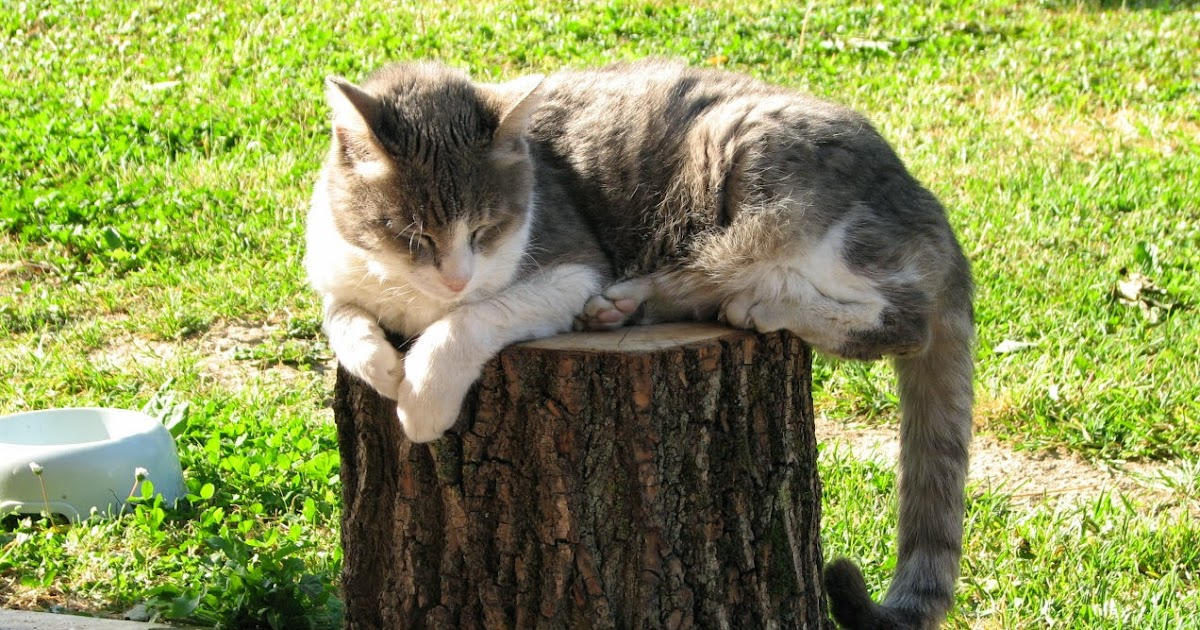
\includegraphics[height=3cm]{img/gatto.jpg}
  \caption{Gatto}
  \label{fig:gatto}
\end{figure}

Il suo istogramma sarà composto, nel seguente modo, ricordano che la
gamma dei colori va da 0 a 255 come espresso in (\ref{sec:rgbcolor}),
la scala del grafico sarà proprio quella.
\begin{figure}[ht!]
  \centering
  \resizebox{15cm}{!}{
  %% Creator: Matplotlib, PGF backend
%%
%% To include the figure in your LaTeX document, write
%%   \input{<filename>.pgf}
%%
%% Make sure the required packages are loaded in your preamble
%%   \usepackage{pgf}
%%
%% Also ensure that all the required font packages are loaded; for instance,
%% the lmodern package is sometimes necessary when using math font.
%%   \usepackage{lmodern}
%%
%% Figures using additional raster images can only be included by \input if
%% they are in the same directory as the main LaTeX file. For loading figures
%% from other directories you can use the `import` package
%%   \usepackage{import}
%%
%% and then include the figures with
%%   \import{<path to file>}{<filename>.pgf}
%%
%% Matplotlib used the following preamble
%%   
%%   \usepackage{fontspec}
%%   \setmainfont{DejaVuSerif.ttf}[Path=\detokenize{/usr/share/matplotlib/mpl-data/fonts/ttf/}]
%%   \setsansfont{DejaVuSans.ttf}[Path=\detokenize{/usr/share/matplotlib/mpl-data/fonts/ttf/}]
%%   \setmonofont{DejaVuSansMono.ttf}[Path=\detokenize{/usr/share/matplotlib/mpl-data/fonts/ttf/}]
%%   \makeatletter\@ifpackageloaded{underscore}{}{\usepackage[strings]{underscore}}\makeatother
%%
\begingroup%
\makeatletter%
\begin{pgfpicture}%
\pgfpathrectangle{\pgfpointorigin}{\pgfqpoint{13.620000in}{6.720000in}}%
\pgfusepath{use as bounding box, clip}%
\begin{pgfscope}%
\pgfsetbuttcap%
\pgfsetmiterjoin%
\definecolor{currentfill}{rgb}{1.000000,1.000000,1.000000}%
\pgfsetfillcolor{currentfill}%
\pgfsetlinewidth{0.000000pt}%
\definecolor{currentstroke}{rgb}{1.000000,1.000000,1.000000}%
\pgfsetstrokecolor{currentstroke}%
\pgfsetdash{}{0pt}%
\pgfpathmoveto{\pgfqpoint{0.000000in}{0.000000in}}%
\pgfpathlineto{\pgfqpoint{13.620000in}{0.000000in}}%
\pgfpathlineto{\pgfqpoint{13.620000in}{6.720000in}}%
\pgfpathlineto{\pgfqpoint{0.000000in}{6.720000in}}%
\pgfpathlineto{\pgfqpoint{0.000000in}{0.000000in}}%
\pgfpathclose%
\pgfusepath{fill}%
\end{pgfscope}%
\begin{pgfscope}%
\pgfsetbuttcap%
\pgfsetmiterjoin%
\definecolor{currentfill}{rgb}{1.000000,1.000000,1.000000}%
\pgfsetfillcolor{currentfill}%
\pgfsetlinewidth{0.000000pt}%
\definecolor{currentstroke}{rgb}{0.000000,0.000000,0.000000}%
\pgfsetstrokecolor{currentstroke}%
\pgfsetstrokeopacity{0.000000}%
\pgfsetdash{}{0pt}%
\pgfpathmoveto{\pgfqpoint{1.702500in}{0.739200in}}%
\pgfpathlineto{\pgfqpoint{12.258000in}{0.739200in}}%
\pgfpathlineto{\pgfqpoint{12.258000in}{5.913600in}}%
\pgfpathlineto{\pgfqpoint{1.702500in}{5.913600in}}%
\pgfpathlineto{\pgfqpoint{1.702500in}{0.739200in}}%
\pgfpathclose%
\pgfusepath{fill}%
\end{pgfscope}%
\begin{pgfscope}%
\pgfpathrectangle{\pgfqpoint{1.702500in}{0.739200in}}{\pgfqpoint{10.555500in}{5.174400in}}%
\pgfusepath{clip}%
\pgfsetbuttcap%
\pgfsetmiterjoin%
\definecolor{currentfill}{rgb}{0.121569,0.466667,0.705882}%
\pgfsetfillcolor{currentfill}%
\pgfsetlinewidth{0.000000pt}%
\definecolor{currentstroke}{rgb}{0.000000,0.000000,0.000000}%
\pgfsetstrokecolor{currentstroke}%
\pgfsetstrokeopacity{0.000000}%
\pgfsetdash{}{0pt}%
\pgfpathmoveto{\pgfqpoint{1.702500in}{0.739200in}}%
\pgfpathlineto{\pgfqpoint{1.743894in}{0.739200in}}%
\pgfpathlineto{\pgfqpoint{1.743894in}{0.808931in}}%
\pgfpathlineto{\pgfqpoint{1.702500in}{0.808931in}}%
\pgfpathlineto{\pgfqpoint{1.702500in}{0.739200in}}%
\pgfpathclose%
\pgfusepath{fill}%
\end{pgfscope}%
\begin{pgfscope}%
\pgfpathrectangle{\pgfqpoint{1.702500in}{0.739200in}}{\pgfqpoint{10.555500in}{5.174400in}}%
\pgfusepath{clip}%
\pgfsetbuttcap%
\pgfsetmiterjoin%
\definecolor{currentfill}{rgb}{0.121569,0.466667,0.705882}%
\pgfsetfillcolor{currentfill}%
\pgfsetlinewidth{0.000000pt}%
\definecolor{currentstroke}{rgb}{0.000000,0.000000,0.000000}%
\pgfsetstrokecolor{currentstroke}%
\pgfsetstrokeopacity{0.000000}%
\pgfsetdash{}{0pt}%
\pgfpathmoveto{\pgfqpoint{1.743894in}{0.739200in}}%
\pgfpathlineto{\pgfqpoint{1.785288in}{0.739200in}}%
\pgfpathlineto{\pgfqpoint{1.785288in}{0.851602in}}%
\pgfpathlineto{\pgfqpoint{1.743894in}{0.851602in}}%
\pgfpathlineto{\pgfqpoint{1.743894in}{0.739200in}}%
\pgfpathclose%
\pgfusepath{fill}%
\end{pgfscope}%
\begin{pgfscope}%
\pgfpathrectangle{\pgfqpoint{1.702500in}{0.739200in}}{\pgfqpoint{10.555500in}{5.174400in}}%
\pgfusepath{clip}%
\pgfsetbuttcap%
\pgfsetmiterjoin%
\definecolor{currentfill}{rgb}{0.121569,0.466667,0.705882}%
\pgfsetfillcolor{currentfill}%
\pgfsetlinewidth{0.000000pt}%
\definecolor{currentstroke}{rgb}{0.000000,0.000000,0.000000}%
\pgfsetstrokecolor{currentstroke}%
\pgfsetstrokeopacity{0.000000}%
\pgfsetdash{}{0pt}%
\pgfpathmoveto{\pgfqpoint{1.785288in}{0.739200in}}%
\pgfpathlineto{\pgfqpoint{1.826682in}{0.739200in}}%
\pgfpathlineto{\pgfqpoint{1.826682in}{0.902599in}}%
\pgfpathlineto{\pgfqpoint{1.785288in}{0.902599in}}%
\pgfpathlineto{\pgfqpoint{1.785288in}{0.739200in}}%
\pgfpathclose%
\pgfusepath{fill}%
\end{pgfscope}%
\begin{pgfscope}%
\pgfpathrectangle{\pgfqpoint{1.702500in}{0.739200in}}{\pgfqpoint{10.555500in}{5.174400in}}%
\pgfusepath{clip}%
\pgfsetbuttcap%
\pgfsetmiterjoin%
\definecolor{currentfill}{rgb}{0.121569,0.466667,0.705882}%
\pgfsetfillcolor{currentfill}%
\pgfsetlinewidth{0.000000pt}%
\definecolor{currentstroke}{rgb}{0.000000,0.000000,0.000000}%
\pgfsetstrokecolor{currentstroke}%
\pgfsetstrokeopacity{0.000000}%
\pgfsetdash{}{0pt}%
\pgfpathmoveto{\pgfqpoint{1.826682in}{0.739200in}}%
\pgfpathlineto{\pgfqpoint{1.868076in}{0.739200in}}%
\pgfpathlineto{\pgfqpoint{1.868076in}{1.016042in}}%
\pgfpathlineto{\pgfqpoint{1.826682in}{1.016042in}}%
\pgfpathlineto{\pgfqpoint{1.826682in}{0.739200in}}%
\pgfpathclose%
\pgfusepath{fill}%
\end{pgfscope}%
\begin{pgfscope}%
\pgfpathrectangle{\pgfqpoint{1.702500in}{0.739200in}}{\pgfqpoint{10.555500in}{5.174400in}}%
\pgfusepath{clip}%
\pgfsetbuttcap%
\pgfsetmiterjoin%
\definecolor{currentfill}{rgb}{0.121569,0.466667,0.705882}%
\pgfsetfillcolor{currentfill}%
\pgfsetlinewidth{0.000000pt}%
\definecolor{currentstroke}{rgb}{0.000000,0.000000,0.000000}%
\pgfsetstrokecolor{currentstroke}%
\pgfsetstrokeopacity{0.000000}%
\pgfsetdash{}{0pt}%
\pgfpathmoveto{\pgfqpoint{1.868076in}{0.739200in}}%
\pgfpathlineto{\pgfqpoint{1.909471in}{0.739200in}}%
\pgfpathlineto{\pgfqpoint{1.909471in}{1.079529in}}%
\pgfpathlineto{\pgfqpoint{1.868076in}{1.079529in}}%
\pgfpathlineto{\pgfqpoint{1.868076in}{0.739200in}}%
\pgfpathclose%
\pgfusepath{fill}%
\end{pgfscope}%
\begin{pgfscope}%
\pgfpathrectangle{\pgfqpoint{1.702500in}{0.739200in}}{\pgfqpoint{10.555500in}{5.174400in}}%
\pgfusepath{clip}%
\pgfsetbuttcap%
\pgfsetmiterjoin%
\definecolor{currentfill}{rgb}{0.121569,0.466667,0.705882}%
\pgfsetfillcolor{currentfill}%
\pgfsetlinewidth{0.000000pt}%
\definecolor{currentstroke}{rgb}{0.000000,0.000000,0.000000}%
\pgfsetstrokecolor{currentstroke}%
\pgfsetstrokeopacity{0.000000}%
\pgfsetdash{}{0pt}%
\pgfpathmoveto{\pgfqpoint{1.909471in}{0.739200in}}%
\pgfpathlineto{\pgfqpoint{1.950865in}{0.739200in}}%
\pgfpathlineto{\pgfqpoint{1.950865in}{1.170075in}}%
\pgfpathlineto{\pgfqpoint{1.909471in}{1.170075in}}%
\pgfpathlineto{\pgfqpoint{1.909471in}{0.739200in}}%
\pgfpathclose%
\pgfusepath{fill}%
\end{pgfscope}%
\begin{pgfscope}%
\pgfpathrectangle{\pgfqpoint{1.702500in}{0.739200in}}{\pgfqpoint{10.555500in}{5.174400in}}%
\pgfusepath{clip}%
\pgfsetbuttcap%
\pgfsetmiterjoin%
\definecolor{currentfill}{rgb}{0.121569,0.466667,0.705882}%
\pgfsetfillcolor{currentfill}%
\pgfsetlinewidth{0.000000pt}%
\definecolor{currentstroke}{rgb}{0.000000,0.000000,0.000000}%
\pgfsetstrokecolor{currentstroke}%
\pgfsetstrokeopacity{0.000000}%
\pgfsetdash{}{0pt}%
\pgfpathmoveto{\pgfqpoint{1.950865in}{0.739200in}}%
\pgfpathlineto{\pgfqpoint{1.992259in}{0.739200in}}%
\pgfpathlineto{\pgfqpoint{1.992259in}{1.340759in}}%
\pgfpathlineto{\pgfqpoint{1.950865in}{1.340759in}}%
\pgfpathlineto{\pgfqpoint{1.950865in}{0.739200in}}%
\pgfpathclose%
\pgfusepath{fill}%
\end{pgfscope}%
\begin{pgfscope}%
\pgfpathrectangle{\pgfqpoint{1.702500in}{0.739200in}}{\pgfqpoint{10.555500in}{5.174400in}}%
\pgfusepath{clip}%
\pgfsetbuttcap%
\pgfsetmiterjoin%
\definecolor{currentfill}{rgb}{0.121569,0.466667,0.705882}%
\pgfsetfillcolor{currentfill}%
\pgfsetlinewidth{0.000000pt}%
\definecolor{currentstroke}{rgb}{0.000000,0.000000,0.000000}%
\pgfsetstrokecolor{currentstroke}%
\pgfsetstrokeopacity{0.000000}%
\pgfsetdash{}{0pt}%
\pgfpathmoveto{\pgfqpoint{1.992259in}{0.739200in}}%
\pgfpathlineto{\pgfqpoint{2.033653in}{0.739200in}}%
\pgfpathlineto{\pgfqpoint{2.033653in}{1.484384in}}%
\pgfpathlineto{\pgfqpoint{1.992259in}{1.484384in}}%
\pgfpathlineto{\pgfqpoint{1.992259in}{0.739200in}}%
\pgfpathclose%
\pgfusepath{fill}%
\end{pgfscope}%
\begin{pgfscope}%
\pgfpathrectangle{\pgfqpoint{1.702500in}{0.739200in}}{\pgfqpoint{10.555500in}{5.174400in}}%
\pgfusepath{clip}%
\pgfsetbuttcap%
\pgfsetmiterjoin%
\definecolor{currentfill}{rgb}{0.121569,0.466667,0.705882}%
\pgfsetfillcolor{currentfill}%
\pgfsetlinewidth{0.000000pt}%
\definecolor{currentstroke}{rgb}{0.000000,0.000000,0.000000}%
\pgfsetstrokecolor{currentstroke}%
\pgfsetstrokeopacity{0.000000}%
\pgfsetdash{}{0pt}%
\pgfpathmoveto{\pgfqpoint{2.033653in}{0.739200in}}%
\pgfpathlineto{\pgfqpoint{2.075047in}{0.739200in}}%
\pgfpathlineto{\pgfqpoint{2.075047in}{1.699822in}}%
\pgfpathlineto{\pgfqpoint{2.033653in}{1.699822in}}%
\pgfpathlineto{\pgfqpoint{2.033653in}{0.739200in}}%
\pgfpathclose%
\pgfusepath{fill}%
\end{pgfscope}%
\begin{pgfscope}%
\pgfpathrectangle{\pgfqpoint{1.702500in}{0.739200in}}{\pgfqpoint{10.555500in}{5.174400in}}%
\pgfusepath{clip}%
\pgfsetbuttcap%
\pgfsetmiterjoin%
\definecolor{currentfill}{rgb}{0.121569,0.466667,0.705882}%
\pgfsetfillcolor{currentfill}%
\pgfsetlinewidth{0.000000pt}%
\definecolor{currentstroke}{rgb}{0.000000,0.000000,0.000000}%
\pgfsetstrokecolor{currentstroke}%
\pgfsetstrokeopacity{0.000000}%
\pgfsetdash{}{0pt}%
\pgfpathmoveto{\pgfqpoint{2.075047in}{0.739200in}}%
\pgfpathlineto{\pgfqpoint{2.116441in}{0.739200in}}%
\pgfpathlineto{\pgfqpoint{2.116441in}{1.847610in}}%
\pgfpathlineto{\pgfqpoint{2.075047in}{1.847610in}}%
\pgfpathlineto{\pgfqpoint{2.075047in}{0.739200in}}%
\pgfpathclose%
\pgfusepath{fill}%
\end{pgfscope}%
\begin{pgfscope}%
\pgfpathrectangle{\pgfqpoint{1.702500in}{0.739200in}}{\pgfqpoint{10.555500in}{5.174400in}}%
\pgfusepath{clip}%
\pgfsetbuttcap%
\pgfsetmiterjoin%
\definecolor{currentfill}{rgb}{0.121569,0.466667,0.705882}%
\pgfsetfillcolor{currentfill}%
\pgfsetlinewidth{0.000000pt}%
\definecolor{currentstroke}{rgb}{0.000000,0.000000,0.000000}%
\pgfsetstrokecolor{currentstroke}%
\pgfsetstrokeopacity{0.000000}%
\pgfsetdash{}{0pt}%
\pgfpathmoveto{\pgfqpoint{2.116441in}{0.739200in}}%
\pgfpathlineto{\pgfqpoint{2.157835in}{0.739200in}}%
\pgfpathlineto{\pgfqpoint{2.157835in}{2.080740in}}%
\pgfpathlineto{\pgfqpoint{2.116441in}{2.080740in}}%
\pgfpathlineto{\pgfqpoint{2.116441in}{0.739200in}}%
\pgfpathclose%
\pgfusepath{fill}%
\end{pgfscope}%
\begin{pgfscope}%
\pgfpathrectangle{\pgfqpoint{1.702500in}{0.739200in}}{\pgfqpoint{10.555500in}{5.174400in}}%
\pgfusepath{clip}%
\pgfsetbuttcap%
\pgfsetmiterjoin%
\definecolor{currentfill}{rgb}{0.121569,0.466667,0.705882}%
\pgfsetfillcolor{currentfill}%
\pgfsetlinewidth{0.000000pt}%
\definecolor{currentstroke}{rgb}{0.000000,0.000000,0.000000}%
\pgfsetstrokecolor{currentstroke}%
\pgfsetstrokeopacity{0.000000}%
\pgfsetdash{}{0pt}%
\pgfpathmoveto{\pgfqpoint{2.157835in}{0.739200in}}%
\pgfpathlineto{\pgfqpoint{2.199229in}{0.739200in}}%
\pgfpathlineto{\pgfqpoint{2.199229in}{2.279525in}}%
\pgfpathlineto{\pgfqpoint{2.157835in}{2.279525in}}%
\pgfpathlineto{\pgfqpoint{2.157835in}{0.739200in}}%
\pgfpathclose%
\pgfusepath{fill}%
\end{pgfscope}%
\begin{pgfscope}%
\pgfpathrectangle{\pgfqpoint{1.702500in}{0.739200in}}{\pgfqpoint{10.555500in}{5.174400in}}%
\pgfusepath{clip}%
\pgfsetbuttcap%
\pgfsetmiterjoin%
\definecolor{currentfill}{rgb}{0.121569,0.466667,0.705882}%
\pgfsetfillcolor{currentfill}%
\pgfsetlinewidth{0.000000pt}%
\definecolor{currentstroke}{rgb}{0.000000,0.000000,0.000000}%
\pgfsetstrokecolor{currentstroke}%
\pgfsetstrokeopacity{0.000000}%
\pgfsetdash{}{0pt}%
\pgfpathmoveto{\pgfqpoint{2.199229in}{0.739200in}}%
\pgfpathlineto{\pgfqpoint{2.240624in}{0.739200in}}%
\pgfpathlineto{\pgfqpoint{2.240624in}{2.503289in}}%
\pgfpathlineto{\pgfqpoint{2.199229in}{2.503289in}}%
\pgfpathlineto{\pgfqpoint{2.199229in}{0.739200in}}%
\pgfpathclose%
\pgfusepath{fill}%
\end{pgfscope}%
\begin{pgfscope}%
\pgfpathrectangle{\pgfqpoint{1.702500in}{0.739200in}}{\pgfqpoint{10.555500in}{5.174400in}}%
\pgfusepath{clip}%
\pgfsetbuttcap%
\pgfsetmiterjoin%
\definecolor{currentfill}{rgb}{0.121569,0.466667,0.705882}%
\pgfsetfillcolor{currentfill}%
\pgfsetlinewidth{0.000000pt}%
\definecolor{currentstroke}{rgb}{0.000000,0.000000,0.000000}%
\pgfsetstrokecolor{currentstroke}%
\pgfsetstrokeopacity{0.000000}%
\pgfsetdash{}{0pt}%
\pgfpathmoveto{\pgfqpoint{2.240624in}{0.739200in}}%
\pgfpathlineto{\pgfqpoint{2.282018in}{0.739200in}}%
\pgfpathlineto{\pgfqpoint{2.282018in}{2.652117in}}%
\pgfpathlineto{\pgfqpoint{2.240624in}{2.652117in}}%
\pgfpathlineto{\pgfqpoint{2.240624in}{0.739200in}}%
\pgfpathclose%
\pgfusepath{fill}%
\end{pgfscope}%
\begin{pgfscope}%
\pgfpathrectangle{\pgfqpoint{1.702500in}{0.739200in}}{\pgfqpoint{10.555500in}{5.174400in}}%
\pgfusepath{clip}%
\pgfsetbuttcap%
\pgfsetmiterjoin%
\definecolor{currentfill}{rgb}{0.121569,0.466667,0.705882}%
\pgfsetfillcolor{currentfill}%
\pgfsetlinewidth{0.000000pt}%
\definecolor{currentstroke}{rgb}{0.000000,0.000000,0.000000}%
\pgfsetstrokecolor{currentstroke}%
\pgfsetstrokeopacity{0.000000}%
\pgfsetdash{}{0pt}%
\pgfpathmoveto{\pgfqpoint{2.282018in}{0.739200in}}%
\pgfpathlineto{\pgfqpoint{2.323412in}{0.739200in}}%
\pgfpathlineto{\pgfqpoint{2.323412in}{2.870677in}}%
\pgfpathlineto{\pgfqpoint{2.282018in}{2.870677in}}%
\pgfpathlineto{\pgfqpoint{2.282018in}{0.739200in}}%
\pgfpathclose%
\pgfusepath{fill}%
\end{pgfscope}%
\begin{pgfscope}%
\pgfpathrectangle{\pgfqpoint{1.702500in}{0.739200in}}{\pgfqpoint{10.555500in}{5.174400in}}%
\pgfusepath{clip}%
\pgfsetbuttcap%
\pgfsetmiterjoin%
\definecolor{currentfill}{rgb}{0.121569,0.466667,0.705882}%
\pgfsetfillcolor{currentfill}%
\pgfsetlinewidth{0.000000pt}%
\definecolor{currentstroke}{rgb}{0.000000,0.000000,0.000000}%
\pgfsetstrokecolor{currentstroke}%
\pgfsetstrokeopacity{0.000000}%
\pgfsetdash{}{0pt}%
\pgfpathmoveto{\pgfqpoint{2.323412in}{0.739200in}}%
\pgfpathlineto{\pgfqpoint{2.364806in}{0.739200in}}%
\pgfpathlineto{\pgfqpoint{2.364806in}{3.053851in}}%
\pgfpathlineto{\pgfqpoint{2.323412in}{3.053851in}}%
\pgfpathlineto{\pgfqpoint{2.323412in}{0.739200in}}%
\pgfpathclose%
\pgfusepath{fill}%
\end{pgfscope}%
\begin{pgfscope}%
\pgfpathrectangle{\pgfqpoint{1.702500in}{0.739200in}}{\pgfqpoint{10.555500in}{5.174400in}}%
\pgfusepath{clip}%
\pgfsetbuttcap%
\pgfsetmiterjoin%
\definecolor{currentfill}{rgb}{0.121569,0.466667,0.705882}%
\pgfsetfillcolor{currentfill}%
\pgfsetlinewidth{0.000000pt}%
\definecolor{currentstroke}{rgb}{0.000000,0.000000,0.000000}%
\pgfsetstrokecolor{currentstroke}%
\pgfsetstrokeopacity{0.000000}%
\pgfsetdash{}{0pt}%
\pgfpathmoveto{\pgfqpoint{2.364806in}{0.739200in}}%
\pgfpathlineto{\pgfqpoint{2.406200in}{0.739200in}}%
\pgfpathlineto{\pgfqpoint{2.406200in}{3.348386in}}%
\pgfpathlineto{\pgfqpoint{2.364806in}{3.348386in}}%
\pgfpathlineto{\pgfqpoint{2.364806in}{0.739200in}}%
\pgfpathclose%
\pgfusepath{fill}%
\end{pgfscope}%
\begin{pgfscope}%
\pgfpathrectangle{\pgfqpoint{1.702500in}{0.739200in}}{\pgfqpoint{10.555500in}{5.174400in}}%
\pgfusepath{clip}%
\pgfsetbuttcap%
\pgfsetmiterjoin%
\definecolor{currentfill}{rgb}{0.121569,0.466667,0.705882}%
\pgfsetfillcolor{currentfill}%
\pgfsetlinewidth{0.000000pt}%
\definecolor{currentstroke}{rgb}{0.000000,0.000000,0.000000}%
\pgfsetstrokecolor{currentstroke}%
\pgfsetstrokeopacity{0.000000}%
\pgfsetdash{}{0pt}%
\pgfpathmoveto{\pgfqpoint{2.406200in}{0.739200in}}%
\pgfpathlineto{\pgfqpoint{2.447594in}{0.739200in}}%
\pgfpathlineto{\pgfqpoint{2.447594in}{3.272411in}}%
\pgfpathlineto{\pgfqpoint{2.406200in}{3.272411in}}%
\pgfpathlineto{\pgfqpoint{2.406200in}{0.739200in}}%
\pgfpathclose%
\pgfusepath{fill}%
\end{pgfscope}%
\begin{pgfscope}%
\pgfpathrectangle{\pgfqpoint{1.702500in}{0.739200in}}{\pgfqpoint{10.555500in}{5.174400in}}%
\pgfusepath{clip}%
\pgfsetbuttcap%
\pgfsetmiterjoin%
\definecolor{currentfill}{rgb}{0.121569,0.466667,0.705882}%
\pgfsetfillcolor{currentfill}%
\pgfsetlinewidth{0.000000pt}%
\definecolor{currentstroke}{rgb}{0.000000,0.000000,0.000000}%
\pgfsetstrokecolor{currentstroke}%
\pgfsetstrokeopacity{0.000000}%
\pgfsetdash{}{0pt}%
\pgfpathmoveto{\pgfqpoint{2.447594in}{0.739200in}}%
\pgfpathlineto{\pgfqpoint{2.488988in}{0.739200in}}%
\pgfpathlineto{\pgfqpoint{2.488988in}{3.453503in}}%
\pgfpathlineto{\pgfqpoint{2.447594in}{3.453503in}}%
\pgfpathlineto{\pgfqpoint{2.447594in}{0.739200in}}%
\pgfpathclose%
\pgfusepath{fill}%
\end{pgfscope}%
\begin{pgfscope}%
\pgfpathrectangle{\pgfqpoint{1.702500in}{0.739200in}}{\pgfqpoint{10.555500in}{5.174400in}}%
\pgfusepath{clip}%
\pgfsetbuttcap%
\pgfsetmiterjoin%
\definecolor{currentfill}{rgb}{0.121569,0.466667,0.705882}%
\pgfsetfillcolor{currentfill}%
\pgfsetlinewidth{0.000000pt}%
\definecolor{currentstroke}{rgb}{0.000000,0.000000,0.000000}%
\pgfsetstrokecolor{currentstroke}%
\pgfsetstrokeopacity{0.000000}%
\pgfsetdash{}{0pt}%
\pgfpathmoveto{\pgfqpoint{2.488988in}{0.739200in}}%
\pgfpathlineto{\pgfqpoint{2.530382in}{0.739200in}}%
\pgfpathlineto{\pgfqpoint{2.530382in}{3.912478in}}%
\pgfpathlineto{\pgfqpoint{2.488988in}{3.912478in}}%
\pgfpathlineto{\pgfqpoint{2.488988in}{0.739200in}}%
\pgfpathclose%
\pgfusepath{fill}%
\end{pgfscope}%
\begin{pgfscope}%
\pgfpathrectangle{\pgfqpoint{1.702500in}{0.739200in}}{\pgfqpoint{10.555500in}{5.174400in}}%
\pgfusepath{clip}%
\pgfsetbuttcap%
\pgfsetmiterjoin%
\definecolor{currentfill}{rgb}{0.121569,0.466667,0.705882}%
\pgfsetfillcolor{currentfill}%
\pgfsetlinewidth{0.000000pt}%
\definecolor{currentstroke}{rgb}{0.000000,0.000000,0.000000}%
\pgfsetstrokecolor{currentstroke}%
\pgfsetstrokeopacity{0.000000}%
\pgfsetdash{}{0pt}%
\pgfpathmoveto{\pgfqpoint{2.530382in}{0.739200in}}%
\pgfpathlineto{\pgfqpoint{2.571776in}{0.739200in}}%
\pgfpathlineto{\pgfqpoint{2.571776in}{3.973883in}}%
\pgfpathlineto{\pgfqpoint{2.530382in}{3.973883in}}%
\pgfpathlineto{\pgfqpoint{2.530382in}{0.739200in}}%
\pgfpathclose%
\pgfusepath{fill}%
\end{pgfscope}%
\begin{pgfscope}%
\pgfpathrectangle{\pgfqpoint{1.702500in}{0.739200in}}{\pgfqpoint{10.555500in}{5.174400in}}%
\pgfusepath{clip}%
\pgfsetbuttcap%
\pgfsetmiterjoin%
\definecolor{currentfill}{rgb}{0.121569,0.466667,0.705882}%
\pgfsetfillcolor{currentfill}%
\pgfsetlinewidth{0.000000pt}%
\definecolor{currentstroke}{rgb}{0.000000,0.000000,0.000000}%
\pgfsetstrokecolor{currentstroke}%
\pgfsetstrokeopacity{0.000000}%
\pgfsetdash{}{0pt}%
\pgfpathmoveto{\pgfqpoint{2.571776in}{0.739200in}}%
\pgfpathlineto{\pgfqpoint{2.613171in}{0.739200in}}%
\pgfpathlineto{\pgfqpoint{2.613171in}{4.054022in}}%
\pgfpathlineto{\pgfqpoint{2.571776in}{4.054022in}}%
\pgfpathlineto{\pgfqpoint{2.571776in}{0.739200in}}%
\pgfpathclose%
\pgfusepath{fill}%
\end{pgfscope}%
\begin{pgfscope}%
\pgfpathrectangle{\pgfqpoint{1.702500in}{0.739200in}}{\pgfqpoint{10.555500in}{5.174400in}}%
\pgfusepath{clip}%
\pgfsetbuttcap%
\pgfsetmiterjoin%
\definecolor{currentfill}{rgb}{0.121569,0.466667,0.705882}%
\pgfsetfillcolor{currentfill}%
\pgfsetlinewidth{0.000000pt}%
\definecolor{currentstroke}{rgb}{0.000000,0.000000,0.000000}%
\pgfsetstrokecolor{currentstroke}%
\pgfsetstrokeopacity{0.000000}%
\pgfsetdash{}{0pt}%
\pgfpathmoveto{\pgfqpoint{2.613171in}{0.739200in}}%
\pgfpathlineto{\pgfqpoint{2.654565in}{0.739200in}}%
\pgfpathlineto{\pgfqpoint{2.654565in}{4.234073in}}%
\pgfpathlineto{\pgfqpoint{2.613171in}{4.234073in}}%
\pgfpathlineto{\pgfqpoint{2.613171in}{0.739200in}}%
\pgfpathclose%
\pgfusepath{fill}%
\end{pgfscope}%
\begin{pgfscope}%
\pgfpathrectangle{\pgfqpoint{1.702500in}{0.739200in}}{\pgfqpoint{10.555500in}{5.174400in}}%
\pgfusepath{clip}%
\pgfsetbuttcap%
\pgfsetmiterjoin%
\definecolor{currentfill}{rgb}{0.121569,0.466667,0.705882}%
\pgfsetfillcolor{currentfill}%
\pgfsetlinewidth{0.000000pt}%
\definecolor{currentstroke}{rgb}{0.000000,0.000000,0.000000}%
\pgfsetstrokecolor{currentstroke}%
\pgfsetstrokeopacity{0.000000}%
\pgfsetdash{}{0pt}%
\pgfpathmoveto{\pgfqpoint{2.654565in}{0.739200in}}%
\pgfpathlineto{\pgfqpoint{2.695959in}{0.739200in}}%
\pgfpathlineto{\pgfqpoint{2.695959in}{4.229910in}}%
\pgfpathlineto{\pgfqpoint{2.654565in}{4.229910in}}%
\pgfpathlineto{\pgfqpoint{2.654565in}{0.739200in}}%
\pgfpathclose%
\pgfusepath{fill}%
\end{pgfscope}%
\begin{pgfscope}%
\pgfpathrectangle{\pgfqpoint{1.702500in}{0.739200in}}{\pgfqpoint{10.555500in}{5.174400in}}%
\pgfusepath{clip}%
\pgfsetbuttcap%
\pgfsetmiterjoin%
\definecolor{currentfill}{rgb}{0.121569,0.466667,0.705882}%
\pgfsetfillcolor{currentfill}%
\pgfsetlinewidth{0.000000pt}%
\definecolor{currentstroke}{rgb}{0.000000,0.000000,0.000000}%
\pgfsetstrokecolor{currentstroke}%
\pgfsetstrokeopacity{0.000000}%
\pgfsetdash{}{0pt}%
\pgfpathmoveto{\pgfqpoint{2.695959in}{0.739200in}}%
\pgfpathlineto{\pgfqpoint{2.737353in}{0.739200in}}%
\pgfpathlineto{\pgfqpoint{2.737353in}{4.451592in}}%
\pgfpathlineto{\pgfqpoint{2.695959in}{4.451592in}}%
\pgfpathlineto{\pgfqpoint{2.695959in}{0.739200in}}%
\pgfpathclose%
\pgfusepath{fill}%
\end{pgfscope}%
\begin{pgfscope}%
\pgfpathrectangle{\pgfqpoint{1.702500in}{0.739200in}}{\pgfqpoint{10.555500in}{5.174400in}}%
\pgfusepath{clip}%
\pgfsetbuttcap%
\pgfsetmiterjoin%
\definecolor{currentfill}{rgb}{0.121569,0.466667,0.705882}%
\pgfsetfillcolor{currentfill}%
\pgfsetlinewidth{0.000000pt}%
\definecolor{currentstroke}{rgb}{0.000000,0.000000,0.000000}%
\pgfsetstrokecolor{currentstroke}%
\pgfsetstrokeopacity{0.000000}%
\pgfsetdash{}{0pt}%
\pgfpathmoveto{\pgfqpoint{2.737353in}{0.739200in}}%
\pgfpathlineto{\pgfqpoint{2.778747in}{0.739200in}}%
\pgfpathlineto{\pgfqpoint{2.778747in}{4.369372in}}%
\pgfpathlineto{\pgfqpoint{2.737353in}{4.369372in}}%
\pgfpathlineto{\pgfqpoint{2.737353in}{0.739200in}}%
\pgfpathclose%
\pgfusepath{fill}%
\end{pgfscope}%
\begin{pgfscope}%
\pgfpathrectangle{\pgfqpoint{1.702500in}{0.739200in}}{\pgfqpoint{10.555500in}{5.174400in}}%
\pgfusepath{clip}%
\pgfsetbuttcap%
\pgfsetmiterjoin%
\definecolor{currentfill}{rgb}{0.121569,0.466667,0.705882}%
\pgfsetfillcolor{currentfill}%
\pgfsetlinewidth{0.000000pt}%
\definecolor{currentstroke}{rgb}{0.000000,0.000000,0.000000}%
\pgfsetstrokecolor{currentstroke}%
\pgfsetstrokeopacity{0.000000}%
\pgfsetdash{}{0pt}%
\pgfpathmoveto{\pgfqpoint{2.778747in}{0.739200in}}%
\pgfpathlineto{\pgfqpoint{2.820141in}{0.739200in}}%
\pgfpathlineto{\pgfqpoint{2.820141in}{4.381861in}}%
\pgfpathlineto{\pgfqpoint{2.778747in}{4.381861in}}%
\pgfpathlineto{\pgfqpoint{2.778747in}{0.739200in}}%
\pgfpathclose%
\pgfusepath{fill}%
\end{pgfscope}%
\begin{pgfscope}%
\pgfpathrectangle{\pgfqpoint{1.702500in}{0.739200in}}{\pgfqpoint{10.555500in}{5.174400in}}%
\pgfusepath{clip}%
\pgfsetbuttcap%
\pgfsetmiterjoin%
\definecolor{currentfill}{rgb}{0.121569,0.466667,0.705882}%
\pgfsetfillcolor{currentfill}%
\pgfsetlinewidth{0.000000pt}%
\definecolor{currentstroke}{rgb}{0.000000,0.000000,0.000000}%
\pgfsetstrokecolor{currentstroke}%
\pgfsetstrokeopacity{0.000000}%
\pgfsetdash{}{0pt}%
\pgfpathmoveto{\pgfqpoint{2.820141in}{0.739200in}}%
\pgfpathlineto{\pgfqpoint{2.861535in}{0.739200in}}%
\pgfpathlineto{\pgfqpoint{2.861535in}{4.601461in}}%
\pgfpathlineto{\pgfqpoint{2.820141in}{4.601461in}}%
\pgfpathlineto{\pgfqpoint{2.820141in}{0.739200in}}%
\pgfpathclose%
\pgfusepath{fill}%
\end{pgfscope}%
\begin{pgfscope}%
\pgfpathrectangle{\pgfqpoint{1.702500in}{0.739200in}}{\pgfqpoint{10.555500in}{5.174400in}}%
\pgfusepath{clip}%
\pgfsetbuttcap%
\pgfsetmiterjoin%
\definecolor{currentfill}{rgb}{0.121569,0.466667,0.705882}%
\pgfsetfillcolor{currentfill}%
\pgfsetlinewidth{0.000000pt}%
\definecolor{currentstroke}{rgb}{0.000000,0.000000,0.000000}%
\pgfsetstrokecolor{currentstroke}%
\pgfsetstrokeopacity{0.000000}%
\pgfsetdash{}{0pt}%
\pgfpathmoveto{\pgfqpoint{2.861535in}{0.739200in}}%
\pgfpathlineto{\pgfqpoint{2.902929in}{0.739200in}}%
\pgfpathlineto{\pgfqpoint{2.902929in}{4.576483in}}%
\pgfpathlineto{\pgfqpoint{2.861535in}{4.576483in}}%
\pgfpathlineto{\pgfqpoint{2.861535in}{0.739200in}}%
\pgfpathclose%
\pgfusepath{fill}%
\end{pgfscope}%
\begin{pgfscope}%
\pgfpathrectangle{\pgfqpoint{1.702500in}{0.739200in}}{\pgfqpoint{10.555500in}{5.174400in}}%
\pgfusepath{clip}%
\pgfsetbuttcap%
\pgfsetmiterjoin%
\definecolor{currentfill}{rgb}{0.121569,0.466667,0.705882}%
\pgfsetfillcolor{currentfill}%
\pgfsetlinewidth{0.000000pt}%
\definecolor{currentstroke}{rgb}{0.000000,0.000000,0.000000}%
\pgfsetstrokecolor{currentstroke}%
\pgfsetstrokeopacity{0.000000}%
\pgfsetdash{}{0pt}%
\pgfpathmoveto{\pgfqpoint{2.902929in}{0.739200in}}%
\pgfpathlineto{\pgfqpoint{2.944324in}{0.739200in}}%
\pgfpathlineto{\pgfqpoint{2.944324in}{4.614991in}}%
\pgfpathlineto{\pgfqpoint{2.902929in}{4.614991in}}%
\pgfpathlineto{\pgfqpoint{2.902929in}{0.739200in}}%
\pgfpathclose%
\pgfusepath{fill}%
\end{pgfscope}%
\begin{pgfscope}%
\pgfpathrectangle{\pgfqpoint{1.702500in}{0.739200in}}{\pgfqpoint{10.555500in}{5.174400in}}%
\pgfusepath{clip}%
\pgfsetbuttcap%
\pgfsetmiterjoin%
\definecolor{currentfill}{rgb}{0.121569,0.466667,0.705882}%
\pgfsetfillcolor{currentfill}%
\pgfsetlinewidth{0.000000pt}%
\definecolor{currentstroke}{rgb}{0.000000,0.000000,0.000000}%
\pgfsetstrokecolor{currentstroke}%
\pgfsetstrokeopacity{0.000000}%
\pgfsetdash{}{0pt}%
\pgfpathmoveto{\pgfqpoint{2.944324in}{0.739200in}}%
\pgfpathlineto{\pgfqpoint{2.985718in}{0.739200in}}%
\pgfpathlineto{\pgfqpoint{2.985718in}{4.618114in}}%
\pgfpathlineto{\pgfqpoint{2.944324in}{4.618114in}}%
\pgfpathlineto{\pgfqpoint{2.944324in}{0.739200in}}%
\pgfpathclose%
\pgfusepath{fill}%
\end{pgfscope}%
\begin{pgfscope}%
\pgfpathrectangle{\pgfqpoint{1.702500in}{0.739200in}}{\pgfqpoint{10.555500in}{5.174400in}}%
\pgfusepath{clip}%
\pgfsetbuttcap%
\pgfsetmiterjoin%
\definecolor{currentfill}{rgb}{0.121569,0.466667,0.705882}%
\pgfsetfillcolor{currentfill}%
\pgfsetlinewidth{0.000000pt}%
\definecolor{currentstroke}{rgb}{0.000000,0.000000,0.000000}%
\pgfsetstrokecolor{currentstroke}%
\pgfsetstrokeopacity{0.000000}%
\pgfsetdash{}{0pt}%
\pgfpathmoveto{\pgfqpoint{2.985718in}{0.739200in}}%
\pgfpathlineto{\pgfqpoint{3.027112in}{0.739200in}}%
\pgfpathlineto{\pgfqpoint{3.027112in}{4.711782in}}%
\pgfpathlineto{\pgfqpoint{2.985718in}{4.711782in}}%
\pgfpathlineto{\pgfqpoint{2.985718in}{0.739200in}}%
\pgfpathclose%
\pgfusepath{fill}%
\end{pgfscope}%
\begin{pgfscope}%
\pgfpathrectangle{\pgfqpoint{1.702500in}{0.739200in}}{\pgfqpoint{10.555500in}{5.174400in}}%
\pgfusepath{clip}%
\pgfsetbuttcap%
\pgfsetmiterjoin%
\definecolor{currentfill}{rgb}{0.121569,0.466667,0.705882}%
\pgfsetfillcolor{currentfill}%
\pgfsetlinewidth{0.000000pt}%
\definecolor{currentstroke}{rgb}{0.000000,0.000000,0.000000}%
\pgfsetstrokecolor{currentstroke}%
\pgfsetstrokeopacity{0.000000}%
\pgfsetdash{}{0pt}%
\pgfpathmoveto{\pgfqpoint{3.027112in}{0.739200in}}%
\pgfpathlineto{\pgfqpoint{3.068506in}{0.739200in}}%
\pgfpathlineto{\pgfqpoint{3.068506in}{4.457837in}}%
\pgfpathlineto{\pgfqpoint{3.027112in}{4.457837in}}%
\pgfpathlineto{\pgfqpoint{3.027112in}{0.739200in}}%
\pgfpathclose%
\pgfusepath{fill}%
\end{pgfscope}%
\begin{pgfscope}%
\pgfpathrectangle{\pgfqpoint{1.702500in}{0.739200in}}{\pgfqpoint{10.555500in}{5.174400in}}%
\pgfusepath{clip}%
\pgfsetbuttcap%
\pgfsetmiterjoin%
\definecolor{currentfill}{rgb}{0.121569,0.466667,0.705882}%
\pgfsetfillcolor{currentfill}%
\pgfsetlinewidth{0.000000pt}%
\definecolor{currentstroke}{rgb}{0.000000,0.000000,0.000000}%
\pgfsetstrokecolor{currentstroke}%
\pgfsetstrokeopacity{0.000000}%
\pgfsetdash{}{0pt}%
\pgfpathmoveto{\pgfqpoint{3.068506in}{0.739200in}}%
\pgfpathlineto{\pgfqpoint{3.109900in}{0.739200in}}%
\pgfpathlineto{\pgfqpoint{3.109900in}{4.678478in}}%
\pgfpathlineto{\pgfqpoint{3.068506in}{4.678478in}}%
\pgfpathlineto{\pgfqpoint{3.068506in}{0.739200in}}%
\pgfpathclose%
\pgfusepath{fill}%
\end{pgfscope}%
\begin{pgfscope}%
\pgfpathrectangle{\pgfqpoint{1.702500in}{0.739200in}}{\pgfqpoint{10.555500in}{5.174400in}}%
\pgfusepath{clip}%
\pgfsetbuttcap%
\pgfsetmiterjoin%
\definecolor{currentfill}{rgb}{0.121569,0.466667,0.705882}%
\pgfsetfillcolor{currentfill}%
\pgfsetlinewidth{0.000000pt}%
\definecolor{currentstroke}{rgb}{0.000000,0.000000,0.000000}%
\pgfsetstrokecolor{currentstroke}%
\pgfsetstrokeopacity{0.000000}%
\pgfsetdash{}{0pt}%
\pgfpathmoveto{\pgfqpoint{3.109900in}{0.739200in}}%
\pgfpathlineto{\pgfqpoint{3.151294in}{0.739200in}}%
\pgfpathlineto{\pgfqpoint{3.151294in}{4.677437in}}%
\pgfpathlineto{\pgfqpoint{3.109900in}{4.677437in}}%
\pgfpathlineto{\pgfqpoint{3.109900in}{0.739200in}}%
\pgfpathclose%
\pgfusepath{fill}%
\end{pgfscope}%
\begin{pgfscope}%
\pgfpathrectangle{\pgfqpoint{1.702500in}{0.739200in}}{\pgfqpoint{10.555500in}{5.174400in}}%
\pgfusepath{clip}%
\pgfsetbuttcap%
\pgfsetmiterjoin%
\definecolor{currentfill}{rgb}{0.121569,0.466667,0.705882}%
\pgfsetfillcolor{currentfill}%
\pgfsetlinewidth{0.000000pt}%
\definecolor{currentstroke}{rgb}{0.000000,0.000000,0.000000}%
\pgfsetstrokecolor{currentstroke}%
\pgfsetstrokeopacity{0.000000}%
\pgfsetdash{}{0pt}%
\pgfpathmoveto{\pgfqpoint{3.151294in}{0.739200in}}%
\pgfpathlineto{\pgfqpoint{3.192688in}{0.739200in}}%
\pgfpathlineto{\pgfqpoint{3.192688in}{4.791921in}}%
\pgfpathlineto{\pgfqpoint{3.151294in}{4.791921in}}%
\pgfpathlineto{\pgfqpoint{3.151294in}{0.739200in}}%
\pgfpathclose%
\pgfusepath{fill}%
\end{pgfscope}%
\begin{pgfscope}%
\pgfpathrectangle{\pgfqpoint{1.702500in}{0.739200in}}{\pgfqpoint{10.555500in}{5.174400in}}%
\pgfusepath{clip}%
\pgfsetbuttcap%
\pgfsetmiterjoin%
\definecolor{currentfill}{rgb}{0.121569,0.466667,0.705882}%
\pgfsetfillcolor{currentfill}%
\pgfsetlinewidth{0.000000pt}%
\definecolor{currentstroke}{rgb}{0.000000,0.000000,0.000000}%
\pgfsetstrokecolor{currentstroke}%
\pgfsetstrokeopacity{0.000000}%
\pgfsetdash{}{0pt}%
\pgfpathmoveto{\pgfqpoint{3.192688in}{0.739200in}}%
\pgfpathlineto{\pgfqpoint{3.234082in}{0.739200in}}%
\pgfpathlineto{\pgfqpoint{3.234082in}{4.645173in}}%
\pgfpathlineto{\pgfqpoint{3.192688in}{4.645173in}}%
\pgfpathlineto{\pgfqpoint{3.192688in}{0.739200in}}%
\pgfpathclose%
\pgfusepath{fill}%
\end{pgfscope}%
\begin{pgfscope}%
\pgfpathrectangle{\pgfqpoint{1.702500in}{0.739200in}}{\pgfqpoint{10.555500in}{5.174400in}}%
\pgfusepath{clip}%
\pgfsetbuttcap%
\pgfsetmiterjoin%
\definecolor{currentfill}{rgb}{0.121569,0.466667,0.705882}%
\pgfsetfillcolor{currentfill}%
\pgfsetlinewidth{0.000000pt}%
\definecolor{currentstroke}{rgb}{0.000000,0.000000,0.000000}%
\pgfsetstrokecolor{currentstroke}%
\pgfsetstrokeopacity{0.000000}%
\pgfsetdash{}{0pt}%
\pgfpathmoveto{\pgfqpoint{3.234082in}{0.739200in}}%
\pgfpathlineto{\pgfqpoint{3.275476in}{0.739200in}}%
\pgfpathlineto{\pgfqpoint{3.275476in}{4.716986in}}%
\pgfpathlineto{\pgfqpoint{3.234082in}{4.716986in}}%
\pgfpathlineto{\pgfqpoint{3.234082in}{0.739200in}}%
\pgfpathclose%
\pgfusepath{fill}%
\end{pgfscope}%
\begin{pgfscope}%
\pgfpathrectangle{\pgfqpoint{1.702500in}{0.739200in}}{\pgfqpoint{10.555500in}{5.174400in}}%
\pgfusepath{clip}%
\pgfsetbuttcap%
\pgfsetmiterjoin%
\definecolor{currentfill}{rgb}{0.121569,0.466667,0.705882}%
\pgfsetfillcolor{currentfill}%
\pgfsetlinewidth{0.000000pt}%
\definecolor{currentstroke}{rgb}{0.000000,0.000000,0.000000}%
\pgfsetstrokecolor{currentstroke}%
\pgfsetstrokeopacity{0.000000}%
\pgfsetdash{}{0pt}%
\pgfpathmoveto{\pgfqpoint{3.275476in}{0.739200in}}%
\pgfpathlineto{\pgfqpoint{3.316871in}{0.739200in}}%
\pgfpathlineto{\pgfqpoint{3.316871in}{4.769024in}}%
\pgfpathlineto{\pgfqpoint{3.275476in}{4.769024in}}%
\pgfpathlineto{\pgfqpoint{3.275476in}{0.739200in}}%
\pgfpathclose%
\pgfusepath{fill}%
\end{pgfscope}%
\begin{pgfscope}%
\pgfpathrectangle{\pgfqpoint{1.702500in}{0.739200in}}{\pgfqpoint{10.555500in}{5.174400in}}%
\pgfusepath{clip}%
\pgfsetbuttcap%
\pgfsetmiterjoin%
\definecolor{currentfill}{rgb}{0.121569,0.466667,0.705882}%
\pgfsetfillcolor{currentfill}%
\pgfsetlinewidth{0.000000pt}%
\definecolor{currentstroke}{rgb}{0.000000,0.000000,0.000000}%
\pgfsetstrokecolor{currentstroke}%
\pgfsetstrokeopacity{0.000000}%
\pgfsetdash{}{0pt}%
\pgfpathmoveto{\pgfqpoint{3.316871in}{0.739200in}}%
\pgfpathlineto{\pgfqpoint{3.358265in}{0.739200in}}%
\pgfpathlineto{\pgfqpoint{3.358265in}{4.806491in}}%
\pgfpathlineto{\pgfqpoint{3.316871in}{4.806491in}}%
\pgfpathlineto{\pgfqpoint{3.316871in}{0.739200in}}%
\pgfpathclose%
\pgfusepath{fill}%
\end{pgfscope}%
\begin{pgfscope}%
\pgfpathrectangle{\pgfqpoint{1.702500in}{0.739200in}}{\pgfqpoint{10.555500in}{5.174400in}}%
\pgfusepath{clip}%
\pgfsetbuttcap%
\pgfsetmiterjoin%
\definecolor{currentfill}{rgb}{0.121569,0.466667,0.705882}%
\pgfsetfillcolor{currentfill}%
\pgfsetlinewidth{0.000000pt}%
\definecolor{currentstroke}{rgb}{0.000000,0.000000,0.000000}%
\pgfsetstrokecolor{currentstroke}%
\pgfsetstrokeopacity{0.000000}%
\pgfsetdash{}{0pt}%
\pgfpathmoveto{\pgfqpoint{3.358265in}{0.739200in}}%
\pgfpathlineto{\pgfqpoint{3.399659in}{0.739200in}}%
\pgfpathlineto{\pgfqpoint{3.399659in}{4.719067in}}%
\pgfpathlineto{\pgfqpoint{3.358265in}{4.719067in}}%
\pgfpathlineto{\pgfqpoint{3.358265in}{0.739200in}}%
\pgfpathclose%
\pgfusepath{fill}%
\end{pgfscope}%
\begin{pgfscope}%
\pgfpathrectangle{\pgfqpoint{1.702500in}{0.739200in}}{\pgfqpoint{10.555500in}{5.174400in}}%
\pgfusepath{clip}%
\pgfsetbuttcap%
\pgfsetmiterjoin%
\definecolor{currentfill}{rgb}{0.121569,0.466667,0.705882}%
\pgfsetfillcolor{currentfill}%
\pgfsetlinewidth{0.000000pt}%
\definecolor{currentstroke}{rgb}{0.000000,0.000000,0.000000}%
\pgfsetstrokecolor{currentstroke}%
\pgfsetstrokeopacity{0.000000}%
\pgfsetdash{}{0pt}%
\pgfpathmoveto{\pgfqpoint{3.399659in}{0.739200in}}%
\pgfpathlineto{\pgfqpoint{3.441053in}{0.739200in}}%
\pgfpathlineto{\pgfqpoint{3.441053in}{4.747168in}}%
\pgfpathlineto{\pgfqpoint{3.399659in}{4.747168in}}%
\pgfpathlineto{\pgfqpoint{3.399659in}{0.739200in}}%
\pgfpathclose%
\pgfusepath{fill}%
\end{pgfscope}%
\begin{pgfscope}%
\pgfpathrectangle{\pgfqpoint{1.702500in}{0.739200in}}{\pgfqpoint{10.555500in}{5.174400in}}%
\pgfusepath{clip}%
\pgfsetbuttcap%
\pgfsetmiterjoin%
\definecolor{currentfill}{rgb}{0.121569,0.466667,0.705882}%
\pgfsetfillcolor{currentfill}%
\pgfsetlinewidth{0.000000pt}%
\definecolor{currentstroke}{rgb}{0.000000,0.000000,0.000000}%
\pgfsetstrokecolor{currentstroke}%
\pgfsetstrokeopacity{0.000000}%
\pgfsetdash{}{0pt}%
\pgfpathmoveto{\pgfqpoint{3.441053in}{0.739200in}}%
\pgfpathlineto{\pgfqpoint{3.482447in}{0.739200in}}%
\pgfpathlineto{\pgfqpoint{3.482447in}{4.777350in}}%
\pgfpathlineto{\pgfqpoint{3.441053in}{4.777350in}}%
\pgfpathlineto{\pgfqpoint{3.441053in}{0.739200in}}%
\pgfpathclose%
\pgfusepath{fill}%
\end{pgfscope}%
\begin{pgfscope}%
\pgfpathrectangle{\pgfqpoint{1.702500in}{0.739200in}}{\pgfqpoint{10.555500in}{5.174400in}}%
\pgfusepath{clip}%
\pgfsetbuttcap%
\pgfsetmiterjoin%
\definecolor{currentfill}{rgb}{0.121569,0.466667,0.705882}%
\pgfsetfillcolor{currentfill}%
\pgfsetlinewidth{0.000000pt}%
\definecolor{currentstroke}{rgb}{0.000000,0.000000,0.000000}%
\pgfsetstrokecolor{currentstroke}%
\pgfsetstrokeopacity{0.000000}%
\pgfsetdash{}{0pt}%
\pgfpathmoveto{\pgfqpoint{3.482447in}{0.739200in}}%
\pgfpathlineto{\pgfqpoint{3.523841in}{0.739200in}}%
\pgfpathlineto{\pgfqpoint{3.523841in}{4.787758in}}%
\pgfpathlineto{\pgfqpoint{3.482447in}{4.787758in}}%
\pgfpathlineto{\pgfqpoint{3.482447in}{0.739200in}}%
\pgfpathclose%
\pgfusepath{fill}%
\end{pgfscope}%
\begin{pgfscope}%
\pgfpathrectangle{\pgfqpoint{1.702500in}{0.739200in}}{\pgfqpoint{10.555500in}{5.174400in}}%
\pgfusepath{clip}%
\pgfsetbuttcap%
\pgfsetmiterjoin%
\definecolor{currentfill}{rgb}{0.121569,0.466667,0.705882}%
\pgfsetfillcolor{currentfill}%
\pgfsetlinewidth{0.000000pt}%
\definecolor{currentstroke}{rgb}{0.000000,0.000000,0.000000}%
\pgfsetstrokecolor{currentstroke}%
\pgfsetstrokeopacity{0.000000}%
\pgfsetdash{}{0pt}%
\pgfpathmoveto{\pgfqpoint{3.523841in}{0.739200in}}%
\pgfpathlineto{\pgfqpoint{3.565235in}{0.739200in}}%
\pgfpathlineto{\pgfqpoint{3.565235in}{4.781513in}}%
\pgfpathlineto{\pgfqpoint{3.523841in}{4.781513in}}%
\pgfpathlineto{\pgfqpoint{3.523841in}{0.739200in}}%
\pgfpathclose%
\pgfusepath{fill}%
\end{pgfscope}%
\begin{pgfscope}%
\pgfpathrectangle{\pgfqpoint{1.702500in}{0.739200in}}{\pgfqpoint{10.555500in}{5.174400in}}%
\pgfusepath{clip}%
\pgfsetbuttcap%
\pgfsetmiterjoin%
\definecolor{currentfill}{rgb}{0.121569,0.466667,0.705882}%
\pgfsetfillcolor{currentfill}%
\pgfsetlinewidth{0.000000pt}%
\definecolor{currentstroke}{rgb}{0.000000,0.000000,0.000000}%
\pgfsetstrokecolor{currentstroke}%
\pgfsetstrokeopacity{0.000000}%
\pgfsetdash{}{0pt}%
\pgfpathmoveto{\pgfqpoint{3.565235in}{0.739200in}}%
\pgfpathlineto{\pgfqpoint{3.606629in}{0.739200in}}%
\pgfpathlineto{\pgfqpoint{3.606629in}{4.907445in}}%
\pgfpathlineto{\pgfqpoint{3.565235in}{4.907445in}}%
\pgfpathlineto{\pgfqpoint{3.565235in}{0.739200in}}%
\pgfpathclose%
\pgfusepath{fill}%
\end{pgfscope}%
\begin{pgfscope}%
\pgfpathrectangle{\pgfqpoint{1.702500in}{0.739200in}}{\pgfqpoint{10.555500in}{5.174400in}}%
\pgfusepath{clip}%
\pgfsetbuttcap%
\pgfsetmiterjoin%
\definecolor{currentfill}{rgb}{0.121569,0.466667,0.705882}%
\pgfsetfillcolor{currentfill}%
\pgfsetlinewidth{0.000000pt}%
\definecolor{currentstroke}{rgb}{0.000000,0.000000,0.000000}%
\pgfsetstrokecolor{currentstroke}%
\pgfsetstrokeopacity{0.000000}%
\pgfsetdash{}{0pt}%
\pgfpathmoveto{\pgfqpoint{3.606629in}{0.739200in}}%
\pgfpathlineto{\pgfqpoint{3.648024in}{0.739200in}}%
\pgfpathlineto{\pgfqpoint{3.648024in}{4.676396in}}%
\pgfpathlineto{\pgfqpoint{3.606629in}{4.676396in}}%
\pgfpathlineto{\pgfqpoint{3.606629in}{0.739200in}}%
\pgfpathclose%
\pgfusepath{fill}%
\end{pgfscope}%
\begin{pgfscope}%
\pgfpathrectangle{\pgfqpoint{1.702500in}{0.739200in}}{\pgfqpoint{10.555500in}{5.174400in}}%
\pgfusepath{clip}%
\pgfsetbuttcap%
\pgfsetmiterjoin%
\definecolor{currentfill}{rgb}{0.121569,0.466667,0.705882}%
\pgfsetfillcolor{currentfill}%
\pgfsetlinewidth{0.000000pt}%
\definecolor{currentstroke}{rgb}{0.000000,0.000000,0.000000}%
\pgfsetstrokecolor{currentstroke}%
\pgfsetstrokeopacity{0.000000}%
\pgfsetdash{}{0pt}%
\pgfpathmoveto{\pgfqpoint{3.648024in}{0.739200in}}%
\pgfpathlineto{\pgfqpoint{3.689418in}{0.739200in}}%
\pgfpathlineto{\pgfqpoint{3.689418in}{4.827306in}}%
\pgfpathlineto{\pgfqpoint{3.648024in}{4.827306in}}%
\pgfpathlineto{\pgfqpoint{3.648024in}{0.739200in}}%
\pgfpathclose%
\pgfusepath{fill}%
\end{pgfscope}%
\begin{pgfscope}%
\pgfpathrectangle{\pgfqpoint{1.702500in}{0.739200in}}{\pgfqpoint{10.555500in}{5.174400in}}%
\pgfusepath{clip}%
\pgfsetbuttcap%
\pgfsetmiterjoin%
\definecolor{currentfill}{rgb}{0.121569,0.466667,0.705882}%
\pgfsetfillcolor{currentfill}%
\pgfsetlinewidth{0.000000pt}%
\definecolor{currentstroke}{rgb}{0.000000,0.000000,0.000000}%
\pgfsetstrokecolor{currentstroke}%
\pgfsetstrokeopacity{0.000000}%
\pgfsetdash{}{0pt}%
\pgfpathmoveto{\pgfqpoint{3.689418in}{0.739200in}}%
\pgfpathlineto{\pgfqpoint{3.730812in}{0.739200in}}%
\pgfpathlineto{\pgfqpoint{3.730812in}{4.827306in}}%
\pgfpathlineto{\pgfqpoint{3.689418in}{4.827306in}}%
\pgfpathlineto{\pgfqpoint{3.689418in}{0.739200in}}%
\pgfpathclose%
\pgfusepath{fill}%
\end{pgfscope}%
\begin{pgfscope}%
\pgfpathrectangle{\pgfqpoint{1.702500in}{0.739200in}}{\pgfqpoint{10.555500in}{5.174400in}}%
\pgfusepath{clip}%
\pgfsetbuttcap%
\pgfsetmiterjoin%
\definecolor{currentfill}{rgb}{0.121569,0.466667,0.705882}%
\pgfsetfillcolor{currentfill}%
\pgfsetlinewidth{0.000000pt}%
\definecolor{currentstroke}{rgb}{0.000000,0.000000,0.000000}%
\pgfsetstrokecolor{currentstroke}%
\pgfsetstrokeopacity{0.000000}%
\pgfsetdash{}{0pt}%
\pgfpathmoveto{\pgfqpoint{3.730812in}{0.739200in}}%
\pgfpathlineto{\pgfqpoint{3.772206in}{0.739200in}}%
\pgfpathlineto{\pgfqpoint{3.772206in}{4.786717in}}%
\pgfpathlineto{\pgfqpoint{3.730812in}{4.786717in}}%
\pgfpathlineto{\pgfqpoint{3.730812in}{0.739200in}}%
\pgfpathclose%
\pgfusepath{fill}%
\end{pgfscope}%
\begin{pgfscope}%
\pgfpathrectangle{\pgfqpoint{1.702500in}{0.739200in}}{\pgfqpoint{10.555500in}{5.174400in}}%
\pgfusepath{clip}%
\pgfsetbuttcap%
\pgfsetmiterjoin%
\definecolor{currentfill}{rgb}{0.121569,0.466667,0.705882}%
\pgfsetfillcolor{currentfill}%
\pgfsetlinewidth{0.000000pt}%
\definecolor{currentstroke}{rgb}{0.000000,0.000000,0.000000}%
\pgfsetstrokecolor{currentstroke}%
\pgfsetstrokeopacity{0.000000}%
\pgfsetdash{}{0pt}%
\pgfpathmoveto{\pgfqpoint{3.772206in}{0.739200in}}%
\pgfpathlineto{\pgfqpoint{3.813600in}{0.739200in}}%
\pgfpathlineto{\pgfqpoint{3.813600in}{4.747168in}}%
\pgfpathlineto{\pgfqpoint{3.772206in}{4.747168in}}%
\pgfpathlineto{\pgfqpoint{3.772206in}{0.739200in}}%
\pgfpathclose%
\pgfusepath{fill}%
\end{pgfscope}%
\begin{pgfscope}%
\pgfpathrectangle{\pgfqpoint{1.702500in}{0.739200in}}{\pgfqpoint{10.555500in}{5.174400in}}%
\pgfusepath{clip}%
\pgfsetbuttcap%
\pgfsetmiterjoin%
\definecolor{currentfill}{rgb}{0.121569,0.466667,0.705882}%
\pgfsetfillcolor{currentfill}%
\pgfsetlinewidth{0.000000pt}%
\definecolor{currentstroke}{rgb}{0.000000,0.000000,0.000000}%
\pgfsetstrokecolor{currentstroke}%
\pgfsetstrokeopacity{0.000000}%
\pgfsetdash{}{0pt}%
\pgfpathmoveto{\pgfqpoint{3.813600in}{0.739200in}}%
\pgfpathlineto{\pgfqpoint{3.854994in}{0.739200in}}%
\pgfpathlineto{\pgfqpoint{3.854994in}{4.777350in}}%
\pgfpathlineto{\pgfqpoint{3.813600in}{4.777350in}}%
\pgfpathlineto{\pgfqpoint{3.813600in}{0.739200in}}%
\pgfpathclose%
\pgfusepath{fill}%
\end{pgfscope}%
\begin{pgfscope}%
\pgfpathrectangle{\pgfqpoint{1.702500in}{0.739200in}}{\pgfqpoint{10.555500in}{5.174400in}}%
\pgfusepath{clip}%
\pgfsetbuttcap%
\pgfsetmiterjoin%
\definecolor{currentfill}{rgb}{0.121569,0.466667,0.705882}%
\pgfsetfillcolor{currentfill}%
\pgfsetlinewidth{0.000000pt}%
\definecolor{currentstroke}{rgb}{0.000000,0.000000,0.000000}%
\pgfsetstrokecolor{currentstroke}%
\pgfsetstrokeopacity{0.000000}%
\pgfsetdash{}{0pt}%
\pgfpathmoveto{\pgfqpoint{3.854994in}{0.739200in}}%
\pgfpathlineto{\pgfqpoint{3.896388in}{0.739200in}}%
\pgfpathlineto{\pgfqpoint{3.896388in}{4.726353in}}%
\pgfpathlineto{\pgfqpoint{3.854994in}{4.726353in}}%
\pgfpathlineto{\pgfqpoint{3.854994in}{0.739200in}}%
\pgfpathclose%
\pgfusepath{fill}%
\end{pgfscope}%
\begin{pgfscope}%
\pgfpathrectangle{\pgfqpoint{1.702500in}{0.739200in}}{\pgfqpoint{10.555500in}{5.174400in}}%
\pgfusepath{clip}%
\pgfsetbuttcap%
\pgfsetmiterjoin%
\definecolor{currentfill}{rgb}{0.121569,0.466667,0.705882}%
\pgfsetfillcolor{currentfill}%
\pgfsetlinewidth{0.000000pt}%
\definecolor{currentstroke}{rgb}{0.000000,0.000000,0.000000}%
\pgfsetstrokecolor{currentstroke}%
\pgfsetstrokeopacity{0.000000}%
\pgfsetdash{}{0pt}%
\pgfpathmoveto{\pgfqpoint{3.896388in}{0.739200in}}%
\pgfpathlineto{\pgfqpoint{3.937782in}{0.739200in}}%
\pgfpathlineto{\pgfqpoint{3.937782in}{4.614991in}}%
\pgfpathlineto{\pgfqpoint{3.896388in}{4.614991in}}%
\pgfpathlineto{\pgfqpoint{3.896388in}{0.739200in}}%
\pgfpathclose%
\pgfusepath{fill}%
\end{pgfscope}%
\begin{pgfscope}%
\pgfpathrectangle{\pgfqpoint{1.702500in}{0.739200in}}{\pgfqpoint{10.555500in}{5.174400in}}%
\pgfusepath{clip}%
\pgfsetbuttcap%
\pgfsetmiterjoin%
\definecolor{currentfill}{rgb}{0.121569,0.466667,0.705882}%
\pgfsetfillcolor{currentfill}%
\pgfsetlinewidth{0.000000pt}%
\definecolor{currentstroke}{rgb}{0.000000,0.000000,0.000000}%
\pgfsetstrokecolor{currentstroke}%
\pgfsetstrokeopacity{0.000000}%
\pgfsetdash{}{0pt}%
\pgfpathmoveto{\pgfqpoint{3.937782in}{0.739200in}}%
\pgfpathlineto{\pgfqpoint{3.979176in}{0.739200in}}%
\pgfpathlineto{\pgfqpoint{3.979176in}{4.765902in}}%
\pgfpathlineto{\pgfqpoint{3.937782in}{4.765902in}}%
\pgfpathlineto{\pgfqpoint{3.937782in}{0.739200in}}%
\pgfpathclose%
\pgfusepath{fill}%
\end{pgfscope}%
\begin{pgfscope}%
\pgfpathrectangle{\pgfqpoint{1.702500in}{0.739200in}}{\pgfqpoint{10.555500in}{5.174400in}}%
\pgfusepath{clip}%
\pgfsetbuttcap%
\pgfsetmiterjoin%
\definecolor{currentfill}{rgb}{0.121569,0.466667,0.705882}%
\pgfsetfillcolor{currentfill}%
\pgfsetlinewidth{0.000000pt}%
\definecolor{currentstroke}{rgb}{0.000000,0.000000,0.000000}%
\pgfsetstrokecolor{currentstroke}%
\pgfsetstrokeopacity{0.000000}%
\pgfsetdash{}{0pt}%
\pgfpathmoveto{\pgfqpoint{3.979176in}{0.739200in}}%
\pgfpathlineto{\pgfqpoint{4.020571in}{0.739200in}}%
\pgfpathlineto{\pgfqpoint{4.020571in}{4.661826in}}%
\pgfpathlineto{\pgfqpoint{3.979176in}{4.661826in}}%
\pgfpathlineto{\pgfqpoint{3.979176in}{0.739200in}}%
\pgfpathclose%
\pgfusepath{fill}%
\end{pgfscope}%
\begin{pgfscope}%
\pgfpathrectangle{\pgfqpoint{1.702500in}{0.739200in}}{\pgfqpoint{10.555500in}{5.174400in}}%
\pgfusepath{clip}%
\pgfsetbuttcap%
\pgfsetmiterjoin%
\definecolor{currentfill}{rgb}{0.121569,0.466667,0.705882}%
\pgfsetfillcolor{currentfill}%
\pgfsetlinewidth{0.000000pt}%
\definecolor{currentstroke}{rgb}{0.000000,0.000000,0.000000}%
\pgfsetstrokecolor{currentstroke}%
\pgfsetstrokeopacity{0.000000}%
\pgfsetdash{}{0pt}%
\pgfpathmoveto{\pgfqpoint{4.020571in}{0.739200in}}%
\pgfpathlineto{\pgfqpoint{4.061965in}{0.739200in}}%
\pgfpathlineto{\pgfqpoint{4.061965in}{4.551505in}}%
\pgfpathlineto{\pgfqpoint{4.020571in}{4.551505in}}%
\pgfpathlineto{\pgfqpoint{4.020571in}{0.739200in}}%
\pgfpathclose%
\pgfusepath{fill}%
\end{pgfscope}%
\begin{pgfscope}%
\pgfpathrectangle{\pgfqpoint{1.702500in}{0.739200in}}{\pgfqpoint{10.555500in}{5.174400in}}%
\pgfusepath{clip}%
\pgfsetbuttcap%
\pgfsetmiterjoin%
\definecolor{currentfill}{rgb}{0.121569,0.466667,0.705882}%
\pgfsetfillcolor{currentfill}%
\pgfsetlinewidth{0.000000pt}%
\definecolor{currentstroke}{rgb}{0.000000,0.000000,0.000000}%
\pgfsetstrokecolor{currentstroke}%
\pgfsetstrokeopacity{0.000000}%
\pgfsetdash{}{0pt}%
\pgfpathmoveto{\pgfqpoint{4.061965in}{0.739200in}}%
\pgfpathlineto{\pgfqpoint{4.103359in}{0.739200in}}%
\pgfpathlineto{\pgfqpoint{4.103359in}{4.700334in}}%
\pgfpathlineto{\pgfqpoint{4.061965in}{4.700334in}}%
\pgfpathlineto{\pgfqpoint{4.061965in}{0.739200in}}%
\pgfpathclose%
\pgfusepath{fill}%
\end{pgfscope}%
\begin{pgfscope}%
\pgfpathrectangle{\pgfqpoint{1.702500in}{0.739200in}}{\pgfqpoint{10.555500in}{5.174400in}}%
\pgfusepath{clip}%
\pgfsetbuttcap%
\pgfsetmiterjoin%
\definecolor{currentfill}{rgb}{0.121569,0.466667,0.705882}%
\pgfsetfillcolor{currentfill}%
\pgfsetlinewidth{0.000000pt}%
\definecolor{currentstroke}{rgb}{0.000000,0.000000,0.000000}%
\pgfsetstrokecolor{currentstroke}%
\pgfsetstrokeopacity{0.000000}%
\pgfsetdash{}{0pt}%
\pgfpathmoveto{\pgfqpoint{4.103359in}{0.739200in}}%
\pgfpathlineto{\pgfqpoint{4.144753in}{0.739200in}}%
\pgfpathlineto{\pgfqpoint{4.144753in}{4.421410in}}%
\pgfpathlineto{\pgfqpoint{4.103359in}{4.421410in}}%
\pgfpathlineto{\pgfqpoint{4.103359in}{0.739200in}}%
\pgfpathclose%
\pgfusepath{fill}%
\end{pgfscope}%
\begin{pgfscope}%
\pgfpathrectangle{\pgfqpoint{1.702500in}{0.739200in}}{\pgfqpoint{10.555500in}{5.174400in}}%
\pgfusepath{clip}%
\pgfsetbuttcap%
\pgfsetmiterjoin%
\definecolor{currentfill}{rgb}{0.121569,0.466667,0.705882}%
\pgfsetfillcolor{currentfill}%
\pgfsetlinewidth{0.000000pt}%
\definecolor{currentstroke}{rgb}{0.000000,0.000000,0.000000}%
\pgfsetstrokecolor{currentstroke}%
\pgfsetstrokeopacity{0.000000}%
\pgfsetdash{}{0pt}%
\pgfpathmoveto{\pgfqpoint{4.144753in}{0.739200in}}%
\pgfpathlineto{\pgfqpoint{4.186147in}{0.739200in}}%
\pgfpathlineto{\pgfqpoint{4.186147in}{4.505712in}}%
\pgfpathlineto{\pgfqpoint{4.144753in}{4.505712in}}%
\pgfpathlineto{\pgfqpoint{4.144753in}{0.739200in}}%
\pgfpathclose%
\pgfusepath{fill}%
\end{pgfscope}%
\begin{pgfscope}%
\pgfpathrectangle{\pgfqpoint{1.702500in}{0.739200in}}{\pgfqpoint{10.555500in}{5.174400in}}%
\pgfusepath{clip}%
\pgfsetbuttcap%
\pgfsetmiterjoin%
\definecolor{currentfill}{rgb}{0.121569,0.466667,0.705882}%
\pgfsetfillcolor{currentfill}%
\pgfsetlinewidth{0.000000pt}%
\definecolor{currentstroke}{rgb}{0.000000,0.000000,0.000000}%
\pgfsetstrokecolor{currentstroke}%
\pgfsetstrokeopacity{0.000000}%
\pgfsetdash{}{0pt}%
\pgfpathmoveto{\pgfqpoint{4.186147in}{0.739200in}}%
\pgfpathlineto{\pgfqpoint{4.227541in}{0.739200in}}%
\pgfpathlineto{\pgfqpoint{4.227541in}{4.510915in}}%
\pgfpathlineto{\pgfqpoint{4.186147in}{4.510915in}}%
\pgfpathlineto{\pgfqpoint{4.186147in}{0.739200in}}%
\pgfpathclose%
\pgfusepath{fill}%
\end{pgfscope}%
\begin{pgfscope}%
\pgfpathrectangle{\pgfqpoint{1.702500in}{0.739200in}}{\pgfqpoint{10.555500in}{5.174400in}}%
\pgfusepath{clip}%
\pgfsetbuttcap%
\pgfsetmiterjoin%
\definecolor{currentfill}{rgb}{0.121569,0.466667,0.705882}%
\pgfsetfillcolor{currentfill}%
\pgfsetlinewidth{0.000000pt}%
\definecolor{currentstroke}{rgb}{0.000000,0.000000,0.000000}%
\pgfsetstrokecolor{currentstroke}%
\pgfsetstrokeopacity{0.000000}%
\pgfsetdash{}{0pt}%
\pgfpathmoveto{\pgfqpoint{4.227541in}{0.739200in}}%
\pgfpathlineto{\pgfqpoint{4.268935in}{0.739200in}}%
\pgfpathlineto{\pgfqpoint{4.268935in}{4.391228in}}%
\pgfpathlineto{\pgfqpoint{4.227541in}{4.391228in}}%
\pgfpathlineto{\pgfqpoint{4.227541in}{0.739200in}}%
\pgfpathclose%
\pgfusepath{fill}%
\end{pgfscope}%
\begin{pgfscope}%
\pgfpathrectangle{\pgfqpoint{1.702500in}{0.739200in}}{\pgfqpoint{10.555500in}{5.174400in}}%
\pgfusepath{clip}%
\pgfsetbuttcap%
\pgfsetmiterjoin%
\definecolor{currentfill}{rgb}{0.121569,0.466667,0.705882}%
\pgfsetfillcolor{currentfill}%
\pgfsetlinewidth{0.000000pt}%
\definecolor{currentstroke}{rgb}{0.000000,0.000000,0.000000}%
\pgfsetstrokecolor{currentstroke}%
\pgfsetstrokeopacity{0.000000}%
\pgfsetdash{}{0pt}%
\pgfpathmoveto{\pgfqpoint{4.268935in}{0.739200in}}%
\pgfpathlineto{\pgfqpoint{4.310329in}{0.739200in}}%
\pgfpathlineto{\pgfqpoint{4.310329in}{4.176831in}}%
\pgfpathlineto{\pgfqpoint{4.268935in}{4.176831in}}%
\pgfpathlineto{\pgfqpoint{4.268935in}{0.739200in}}%
\pgfpathclose%
\pgfusepath{fill}%
\end{pgfscope}%
\begin{pgfscope}%
\pgfpathrectangle{\pgfqpoint{1.702500in}{0.739200in}}{\pgfqpoint{10.555500in}{5.174400in}}%
\pgfusepath{clip}%
\pgfsetbuttcap%
\pgfsetmiterjoin%
\definecolor{currentfill}{rgb}{0.121569,0.466667,0.705882}%
\pgfsetfillcolor{currentfill}%
\pgfsetlinewidth{0.000000pt}%
\definecolor{currentstroke}{rgb}{0.000000,0.000000,0.000000}%
\pgfsetstrokecolor{currentstroke}%
\pgfsetstrokeopacity{0.000000}%
\pgfsetdash{}{0pt}%
\pgfpathmoveto{\pgfqpoint{4.310329in}{0.739200in}}%
\pgfpathlineto{\pgfqpoint{4.351724in}{0.739200in}}%
\pgfpathlineto{\pgfqpoint{4.351724in}{4.209095in}}%
\pgfpathlineto{\pgfqpoint{4.310329in}{4.209095in}}%
\pgfpathlineto{\pgfqpoint{4.310329in}{0.739200in}}%
\pgfpathclose%
\pgfusepath{fill}%
\end{pgfscope}%
\begin{pgfscope}%
\pgfpathrectangle{\pgfqpoint{1.702500in}{0.739200in}}{\pgfqpoint{10.555500in}{5.174400in}}%
\pgfusepath{clip}%
\pgfsetbuttcap%
\pgfsetmiterjoin%
\definecolor{currentfill}{rgb}{0.121569,0.466667,0.705882}%
\pgfsetfillcolor{currentfill}%
\pgfsetlinewidth{0.000000pt}%
\definecolor{currentstroke}{rgb}{0.000000,0.000000,0.000000}%
\pgfsetstrokecolor{currentstroke}%
\pgfsetstrokeopacity{0.000000}%
\pgfsetdash{}{0pt}%
\pgfpathmoveto{\pgfqpoint{4.351724in}{0.739200in}}%
\pgfpathlineto{\pgfqpoint{4.393118in}{0.739200in}}%
\pgfpathlineto{\pgfqpoint{4.393118in}{4.225747in}}%
\pgfpathlineto{\pgfqpoint{4.351724in}{4.225747in}}%
\pgfpathlineto{\pgfqpoint{4.351724in}{0.739200in}}%
\pgfpathclose%
\pgfusepath{fill}%
\end{pgfscope}%
\begin{pgfscope}%
\pgfpathrectangle{\pgfqpoint{1.702500in}{0.739200in}}{\pgfqpoint{10.555500in}{5.174400in}}%
\pgfusepath{clip}%
\pgfsetbuttcap%
\pgfsetmiterjoin%
\definecolor{currentfill}{rgb}{0.121569,0.466667,0.705882}%
\pgfsetfillcolor{currentfill}%
\pgfsetlinewidth{0.000000pt}%
\definecolor{currentstroke}{rgb}{0.000000,0.000000,0.000000}%
\pgfsetstrokecolor{currentstroke}%
\pgfsetstrokeopacity{0.000000}%
\pgfsetdash{}{0pt}%
\pgfpathmoveto{\pgfqpoint{4.393118in}{0.739200in}}%
\pgfpathlineto{\pgfqpoint{4.434512in}{0.739200in}}%
\pgfpathlineto{\pgfqpoint{4.434512in}{4.148731in}}%
\pgfpathlineto{\pgfqpoint{4.393118in}{4.148731in}}%
\pgfpathlineto{\pgfqpoint{4.393118in}{0.739200in}}%
\pgfpathclose%
\pgfusepath{fill}%
\end{pgfscope}%
\begin{pgfscope}%
\pgfpathrectangle{\pgfqpoint{1.702500in}{0.739200in}}{\pgfqpoint{10.555500in}{5.174400in}}%
\pgfusepath{clip}%
\pgfsetbuttcap%
\pgfsetmiterjoin%
\definecolor{currentfill}{rgb}{0.121569,0.466667,0.705882}%
\pgfsetfillcolor{currentfill}%
\pgfsetlinewidth{0.000000pt}%
\definecolor{currentstroke}{rgb}{0.000000,0.000000,0.000000}%
\pgfsetstrokecolor{currentstroke}%
\pgfsetstrokeopacity{0.000000}%
\pgfsetdash{}{0pt}%
\pgfpathmoveto{\pgfqpoint{4.434512in}{0.739200in}}%
\pgfpathlineto{\pgfqpoint{4.475906in}{0.739200in}}%
\pgfpathlineto{\pgfqpoint{4.475906in}{4.088367in}}%
\pgfpathlineto{\pgfqpoint{4.434512in}{4.088367in}}%
\pgfpathlineto{\pgfqpoint{4.434512in}{0.739200in}}%
\pgfpathclose%
\pgfusepath{fill}%
\end{pgfscope}%
\begin{pgfscope}%
\pgfpathrectangle{\pgfqpoint{1.702500in}{0.739200in}}{\pgfqpoint{10.555500in}{5.174400in}}%
\pgfusepath{clip}%
\pgfsetbuttcap%
\pgfsetmiterjoin%
\definecolor{currentfill}{rgb}{0.121569,0.466667,0.705882}%
\pgfsetfillcolor{currentfill}%
\pgfsetlinewidth{0.000000pt}%
\definecolor{currentstroke}{rgb}{0.000000,0.000000,0.000000}%
\pgfsetstrokecolor{currentstroke}%
\pgfsetstrokeopacity{0.000000}%
\pgfsetdash{}{0pt}%
\pgfpathmoveto{\pgfqpoint{4.475906in}{0.739200in}}%
\pgfpathlineto{\pgfqpoint{4.517300in}{0.739200in}}%
\pgfpathlineto{\pgfqpoint{4.517300in}{4.058185in}}%
\pgfpathlineto{\pgfqpoint{4.475906in}{4.058185in}}%
\pgfpathlineto{\pgfqpoint{4.475906in}{0.739200in}}%
\pgfpathclose%
\pgfusepath{fill}%
\end{pgfscope}%
\begin{pgfscope}%
\pgfpathrectangle{\pgfqpoint{1.702500in}{0.739200in}}{\pgfqpoint{10.555500in}{5.174400in}}%
\pgfusepath{clip}%
\pgfsetbuttcap%
\pgfsetmiterjoin%
\definecolor{currentfill}{rgb}{0.121569,0.466667,0.705882}%
\pgfsetfillcolor{currentfill}%
\pgfsetlinewidth{0.000000pt}%
\definecolor{currentstroke}{rgb}{0.000000,0.000000,0.000000}%
\pgfsetstrokecolor{currentstroke}%
\pgfsetstrokeopacity{0.000000}%
\pgfsetdash{}{0pt}%
\pgfpathmoveto{\pgfqpoint{4.517300in}{0.739200in}}%
\pgfpathlineto{\pgfqpoint{4.558694in}{0.739200in}}%
\pgfpathlineto{\pgfqpoint{4.558694in}{3.897907in}}%
\pgfpathlineto{\pgfqpoint{4.517300in}{3.897907in}}%
\pgfpathlineto{\pgfqpoint{4.517300in}{0.739200in}}%
\pgfpathclose%
\pgfusepath{fill}%
\end{pgfscope}%
\begin{pgfscope}%
\pgfpathrectangle{\pgfqpoint{1.702500in}{0.739200in}}{\pgfqpoint{10.555500in}{5.174400in}}%
\pgfusepath{clip}%
\pgfsetbuttcap%
\pgfsetmiterjoin%
\definecolor{currentfill}{rgb}{0.121569,0.466667,0.705882}%
\pgfsetfillcolor{currentfill}%
\pgfsetlinewidth{0.000000pt}%
\definecolor{currentstroke}{rgb}{0.000000,0.000000,0.000000}%
\pgfsetstrokecolor{currentstroke}%
\pgfsetstrokeopacity{0.000000}%
\pgfsetdash{}{0pt}%
\pgfpathmoveto{\pgfqpoint{4.558694in}{0.739200in}}%
\pgfpathlineto{\pgfqpoint{4.600088in}{0.739200in}}%
\pgfpathlineto{\pgfqpoint{4.600088in}{3.782383in}}%
\pgfpathlineto{\pgfqpoint{4.558694in}{3.782383in}}%
\pgfpathlineto{\pgfqpoint{4.558694in}{0.739200in}}%
\pgfpathclose%
\pgfusepath{fill}%
\end{pgfscope}%
\begin{pgfscope}%
\pgfpathrectangle{\pgfqpoint{1.702500in}{0.739200in}}{\pgfqpoint{10.555500in}{5.174400in}}%
\pgfusepath{clip}%
\pgfsetbuttcap%
\pgfsetmiterjoin%
\definecolor{currentfill}{rgb}{0.121569,0.466667,0.705882}%
\pgfsetfillcolor{currentfill}%
\pgfsetlinewidth{0.000000pt}%
\definecolor{currentstroke}{rgb}{0.000000,0.000000,0.000000}%
\pgfsetstrokecolor{currentstroke}%
\pgfsetstrokeopacity{0.000000}%
\pgfsetdash{}{0pt}%
\pgfpathmoveto{\pgfqpoint{4.600088in}{0.739200in}}%
\pgfpathlineto{\pgfqpoint{4.641482in}{0.739200in}}%
\pgfpathlineto{\pgfqpoint{4.641482in}{3.831299in}}%
\pgfpathlineto{\pgfqpoint{4.600088in}{3.831299in}}%
\pgfpathlineto{\pgfqpoint{4.600088in}{0.739200in}}%
\pgfpathclose%
\pgfusepath{fill}%
\end{pgfscope}%
\begin{pgfscope}%
\pgfpathrectangle{\pgfqpoint{1.702500in}{0.739200in}}{\pgfqpoint{10.555500in}{5.174400in}}%
\pgfusepath{clip}%
\pgfsetbuttcap%
\pgfsetmiterjoin%
\definecolor{currentfill}{rgb}{0.121569,0.466667,0.705882}%
\pgfsetfillcolor{currentfill}%
\pgfsetlinewidth{0.000000pt}%
\definecolor{currentstroke}{rgb}{0.000000,0.000000,0.000000}%
\pgfsetstrokecolor{currentstroke}%
\pgfsetstrokeopacity{0.000000}%
\pgfsetdash{}{0pt}%
\pgfpathmoveto{\pgfqpoint{4.641482in}{0.739200in}}%
\pgfpathlineto{\pgfqpoint{4.682876in}{0.739200in}}%
\pgfpathlineto{\pgfqpoint{4.682876in}{3.722019in}}%
\pgfpathlineto{\pgfqpoint{4.641482in}{3.722019in}}%
\pgfpathlineto{\pgfqpoint{4.641482in}{0.739200in}}%
\pgfpathclose%
\pgfusepath{fill}%
\end{pgfscope}%
\begin{pgfscope}%
\pgfpathrectangle{\pgfqpoint{1.702500in}{0.739200in}}{\pgfqpoint{10.555500in}{5.174400in}}%
\pgfusepath{clip}%
\pgfsetbuttcap%
\pgfsetmiterjoin%
\definecolor{currentfill}{rgb}{0.121569,0.466667,0.705882}%
\pgfsetfillcolor{currentfill}%
\pgfsetlinewidth{0.000000pt}%
\definecolor{currentstroke}{rgb}{0.000000,0.000000,0.000000}%
\pgfsetstrokecolor{currentstroke}%
\pgfsetstrokeopacity{0.000000}%
\pgfsetdash{}{0pt}%
\pgfpathmoveto{\pgfqpoint{4.682876in}{0.739200in}}%
\pgfpathlineto{\pgfqpoint{4.724271in}{0.739200in}}%
\pgfpathlineto{\pgfqpoint{4.724271in}{3.719937in}}%
\pgfpathlineto{\pgfqpoint{4.682876in}{3.719937in}}%
\pgfpathlineto{\pgfqpoint{4.682876in}{0.739200in}}%
\pgfpathclose%
\pgfusepath{fill}%
\end{pgfscope}%
\begin{pgfscope}%
\pgfpathrectangle{\pgfqpoint{1.702500in}{0.739200in}}{\pgfqpoint{10.555500in}{5.174400in}}%
\pgfusepath{clip}%
\pgfsetbuttcap%
\pgfsetmiterjoin%
\definecolor{currentfill}{rgb}{0.121569,0.466667,0.705882}%
\pgfsetfillcolor{currentfill}%
\pgfsetlinewidth{0.000000pt}%
\definecolor{currentstroke}{rgb}{0.000000,0.000000,0.000000}%
\pgfsetstrokecolor{currentstroke}%
\pgfsetstrokeopacity{0.000000}%
\pgfsetdash{}{0pt}%
\pgfpathmoveto{\pgfqpoint{4.724271in}{0.739200in}}%
\pgfpathlineto{\pgfqpoint{4.765665in}{0.739200in}}%
\pgfpathlineto{\pgfqpoint{4.765665in}{3.562783in}}%
\pgfpathlineto{\pgfqpoint{4.724271in}{3.562783in}}%
\pgfpathlineto{\pgfqpoint{4.724271in}{0.739200in}}%
\pgfpathclose%
\pgfusepath{fill}%
\end{pgfscope}%
\begin{pgfscope}%
\pgfpathrectangle{\pgfqpoint{1.702500in}{0.739200in}}{\pgfqpoint{10.555500in}{5.174400in}}%
\pgfusepath{clip}%
\pgfsetbuttcap%
\pgfsetmiterjoin%
\definecolor{currentfill}{rgb}{0.121569,0.466667,0.705882}%
\pgfsetfillcolor{currentfill}%
\pgfsetlinewidth{0.000000pt}%
\definecolor{currentstroke}{rgb}{0.000000,0.000000,0.000000}%
\pgfsetstrokecolor{currentstroke}%
\pgfsetstrokeopacity{0.000000}%
\pgfsetdash{}{0pt}%
\pgfpathmoveto{\pgfqpoint{4.765665in}{0.739200in}}%
\pgfpathlineto{\pgfqpoint{4.807059in}{0.739200in}}%
\pgfpathlineto{\pgfqpoint{4.807059in}{3.557579in}}%
\pgfpathlineto{\pgfqpoint{4.765665in}{3.557579in}}%
\pgfpathlineto{\pgfqpoint{4.765665in}{0.739200in}}%
\pgfpathclose%
\pgfusepath{fill}%
\end{pgfscope}%
\begin{pgfscope}%
\pgfpathrectangle{\pgfqpoint{1.702500in}{0.739200in}}{\pgfqpoint{10.555500in}{5.174400in}}%
\pgfusepath{clip}%
\pgfsetbuttcap%
\pgfsetmiterjoin%
\definecolor{currentfill}{rgb}{0.121569,0.466667,0.705882}%
\pgfsetfillcolor{currentfill}%
\pgfsetlinewidth{0.000000pt}%
\definecolor{currentstroke}{rgb}{0.000000,0.000000,0.000000}%
\pgfsetstrokecolor{currentstroke}%
\pgfsetstrokeopacity{0.000000}%
\pgfsetdash{}{0pt}%
\pgfpathmoveto{\pgfqpoint{4.807059in}{0.739200in}}%
\pgfpathlineto{\pgfqpoint{4.848453in}{0.739200in}}%
\pgfpathlineto{\pgfqpoint{4.848453in}{3.627310in}}%
\pgfpathlineto{\pgfqpoint{4.807059in}{3.627310in}}%
\pgfpathlineto{\pgfqpoint{4.807059in}{0.739200in}}%
\pgfpathclose%
\pgfusepath{fill}%
\end{pgfscope}%
\begin{pgfscope}%
\pgfpathrectangle{\pgfqpoint{1.702500in}{0.739200in}}{\pgfqpoint{10.555500in}{5.174400in}}%
\pgfusepath{clip}%
\pgfsetbuttcap%
\pgfsetmiterjoin%
\definecolor{currentfill}{rgb}{0.121569,0.466667,0.705882}%
\pgfsetfillcolor{currentfill}%
\pgfsetlinewidth{0.000000pt}%
\definecolor{currentstroke}{rgb}{0.000000,0.000000,0.000000}%
\pgfsetstrokecolor{currentstroke}%
\pgfsetstrokeopacity{0.000000}%
\pgfsetdash{}{0pt}%
\pgfpathmoveto{\pgfqpoint{4.848453in}{0.739200in}}%
\pgfpathlineto{\pgfqpoint{4.889847in}{0.739200in}}%
\pgfpathlineto{\pgfqpoint{4.889847in}{3.537804in}}%
\pgfpathlineto{\pgfqpoint{4.848453in}{3.537804in}}%
\pgfpathlineto{\pgfqpoint{4.848453in}{0.739200in}}%
\pgfpathclose%
\pgfusepath{fill}%
\end{pgfscope}%
\begin{pgfscope}%
\pgfpathrectangle{\pgfqpoint{1.702500in}{0.739200in}}{\pgfqpoint{10.555500in}{5.174400in}}%
\pgfusepath{clip}%
\pgfsetbuttcap%
\pgfsetmiterjoin%
\definecolor{currentfill}{rgb}{0.121569,0.466667,0.705882}%
\pgfsetfillcolor{currentfill}%
\pgfsetlinewidth{0.000000pt}%
\definecolor{currentstroke}{rgb}{0.000000,0.000000,0.000000}%
\pgfsetstrokecolor{currentstroke}%
\pgfsetstrokeopacity{0.000000}%
\pgfsetdash{}{0pt}%
\pgfpathmoveto{\pgfqpoint{4.889847in}{0.739200in}}%
\pgfpathlineto{\pgfqpoint{4.931241in}{0.739200in}}%
\pgfpathlineto{\pgfqpoint{4.931241in}{3.506582in}}%
\pgfpathlineto{\pgfqpoint{4.889847in}{3.506582in}}%
\pgfpathlineto{\pgfqpoint{4.889847in}{0.739200in}}%
\pgfpathclose%
\pgfusepath{fill}%
\end{pgfscope}%
\begin{pgfscope}%
\pgfpathrectangle{\pgfqpoint{1.702500in}{0.739200in}}{\pgfqpoint{10.555500in}{5.174400in}}%
\pgfusepath{clip}%
\pgfsetbuttcap%
\pgfsetmiterjoin%
\definecolor{currentfill}{rgb}{0.121569,0.466667,0.705882}%
\pgfsetfillcolor{currentfill}%
\pgfsetlinewidth{0.000000pt}%
\definecolor{currentstroke}{rgb}{0.000000,0.000000,0.000000}%
\pgfsetstrokecolor{currentstroke}%
\pgfsetstrokeopacity{0.000000}%
\pgfsetdash{}{0pt}%
\pgfpathmoveto{\pgfqpoint{4.931241in}{0.739200in}}%
\pgfpathlineto{\pgfqpoint{4.972635in}{0.739200in}}%
\pgfpathlineto{\pgfqpoint{4.972635in}{3.551334in}}%
\pgfpathlineto{\pgfqpoint{4.931241in}{3.551334in}}%
\pgfpathlineto{\pgfqpoint{4.931241in}{0.739200in}}%
\pgfpathclose%
\pgfusepath{fill}%
\end{pgfscope}%
\begin{pgfscope}%
\pgfpathrectangle{\pgfqpoint{1.702500in}{0.739200in}}{\pgfqpoint{10.555500in}{5.174400in}}%
\pgfusepath{clip}%
\pgfsetbuttcap%
\pgfsetmiterjoin%
\definecolor{currentfill}{rgb}{0.121569,0.466667,0.705882}%
\pgfsetfillcolor{currentfill}%
\pgfsetlinewidth{0.000000pt}%
\definecolor{currentstroke}{rgb}{0.000000,0.000000,0.000000}%
\pgfsetstrokecolor{currentstroke}%
\pgfsetstrokeopacity{0.000000}%
\pgfsetdash{}{0pt}%
\pgfpathmoveto{\pgfqpoint{4.972635in}{0.739200in}}%
\pgfpathlineto{\pgfqpoint{5.014029in}{0.739200in}}%
\pgfpathlineto{\pgfqpoint{5.014029in}{3.549253in}}%
\pgfpathlineto{\pgfqpoint{4.972635in}{3.549253in}}%
\pgfpathlineto{\pgfqpoint{4.972635in}{0.739200in}}%
\pgfpathclose%
\pgfusepath{fill}%
\end{pgfscope}%
\begin{pgfscope}%
\pgfpathrectangle{\pgfqpoint{1.702500in}{0.739200in}}{\pgfqpoint{10.555500in}{5.174400in}}%
\pgfusepath{clip}%
\pgfsetbuttcap%
\pgfsetmiterjoin%
\definecolor{currentfill}{rgb}{0.121569,0.466667,0.705882}%
\pgfsetfillcolor{currentfill}%
\pgfsetlinewidth{0.000000pt}%
\definecolor{currentstroke}{rgb}{0.000000,0.000000,0.000000}%
\pgfsetstrokecolor{currentstroke}%
\pgfsetstrokeopacity{0.000000}%
\pgfsetdash{}{0pt}%
\pgfpathmoveto{\pgfqpoint{5.014029in}{0.739200in}}%
\pgfpathlineto{\pgfqpoint{5.055424in}{0.739200in}}%
\pgfpathlineto{\pgfqpoint{5.055424in}{3.331734in}}%
\pgfpathlineto{\pgfqpoint{5.014029in}{3.331734in}}%
\pgfpathlineto{\pgfqpoint{5.014029in}{0.739200in}}%
\pgfpathclose%
\pgfusepath{fill}%
\end{pgfscope}%
\begin{pgfscope}%
\pgfpathrectangle{\pgfqpoint{1.702500in}{0.739200in}}{\pgfqpoint{10.555500in}{5.174400in}}%
\pgfusepath{clip}%
\pgfsetbuttcap%
\pgfsetmiterjoin%
\definecolor{currentfill}{rgb}{0.121569,0.466667,0.705882}%
\pgfsetfillcolor{currentfill}%
\pgfsetlinewidth{0.000000pt}%
\definecolor{currentstroke}{rgb}{0.000000,0.000000,0.000000}%
\pgfsetstrokecolor{currentstroke}%
\pgfsetstrokeopacity{0.000000}%
\pgfsetdash{}{0pt}%
\pgfpathmoveto{\pgfqpoint{5.055424in}{0.739200in}}%
\pgfpathlineto{\pgfqpoint{5.096818in}{0.739200in}}%
\pgfpathlineto{\pgfqpoint{5.096818in}{3.351508in}}%
\pgfpathlineto{\pgfqpoint{5.055424in}{3.351508in}}%
\pgfpathlineto{\pgfqpoint{5.055424in}{0.739200in}}%
\pgfpathclose%
\pgfusepath{fill}%
\end{pgfscope}%
\begin{pgfscope}%
\pgfpathrectangle{\pgfqpoint{1.702500in}{0.739200in}}{\pgfqpoint{10.555500in}{5.174400in}}%
\pgfusepath{clip}%
\pgfsetbuttcap%
\pgfsetmiterjoin%
\definecolor{currentfill}{rgb}{0.121569,0.466667,0.705882}%
\pgfsetfillcolor{currentfill}%
\pgfsetlinewidth{0.000000pt}%
\definecolor{currentstroke}{rgb}{0.000000,0.000000,0.000000}%
\pgfsetstrokecolor{currentstroke}%
\pgfsetstrokeopacity{0.000000}%
\pgfsetdash{}{0pt}%
\pgfpathmoveto{\pgfqpoint{5.096818in}{0.739200in}}%
\pgfpathlineto{\pgfqpoint{5.138212in}{0.739200in}}%
\pgfpathlineto{\pgfqpoint{5.138212in}{3.330693in}}%
\pgfpathlineto{\pgfqpoint{5.096818in}{3.330693in}}%
\pgfpathlineto{\pgfqpoint{5.096818in}{0.739200in}}%
\pgfpathclose%
\pgfusepath{fill}%
\end{pgfscope}%
\begin{pgfscope}%
\pgfpathrectangle{\pgfqpoint{1.702500in}{0.739200in}}{\pgfqpoint{10.555500in}{5.174400in}}%
\pgfusepath{clip}%
\pgfsetbuttcap%
\pgfsetmiterjoin%
\definecolor{currentfill}{rgb}{0.121569,0.466667,0.705882}%
\pgfsetfillcolor{currentfill}%
\pgfsetlinewidth{0.000000pt}%
\definecolor{currentstroke}{rgb}{0.000000,0.000000,0.000000}%
\pgfsetstrokecolor{currentstroke}%
\pgfsetstrokeopacity{0.000000}%
\pgfsetdash{}{0pt}%
\pgfpathmoveto{\pgfqpoint{5.138212in}{0.739200in}}%
\pgfpathlineto{\pgfqpoint{5.179606in}{0.739200in}}%
\pgfpathlineto{\pgfqpoint{5.179606in}{3.352549in}}%
\pgfpathlineto{\pgfqpoint{5.138212in}{3.352549in}}%
\pgfpathlineto{\pgfqpoint{5.138212in}{0.739200in}}%
\pgfpathclose%
\pgfusepath{fill}%
\end{pgfscope}%
\begin{pgfscope}%
\pgfpathrectangle{\pgfqpoint{1.702500in}{0.739200in}}{\pgfqpoint{10.555500in}{5.174400in}}%
\pgfusepath{clip}%
\pgfsetbuttcap%
\pgfsetmiterjoin%
\definecolor{currentfill}{rgb}{0.121569,0.466667,0.705882}%
\pgfsetfillcolor{currentfill}%
\pgfsetlinewidth{0.000000pt}%
\definecolor{currentstroke}{rgb}{0.000000,0.000000,0.000000}%
\pgfsetstrokecolor{currentstroke}%
\pgfsetstrokeopacity{0.000000}%
\pgfsetdash{}{0pt}%
\pgfpathmoveto{\pgfqpoint{5.179606in}{0.739200in}}%
\pgfpathlineto{\pgfqpoint{5.221000in}{0.739200in}}%
\pgfpathlineto{\pgfqpoint{5.221000in}{3.330693in}}%
\pgfpathlineto{\pgfqpoint{5.179606in}{3.330693in}}%
\pgfpathlineto{\pgfqpoint{5.179606in}{0.739200in}}%
\pgfpathclose%
\pgfusepath{fill}%
\end{pgfscope}%
\begin{pgfscope}%
\pgfpathrectangle{\pgfqpoint{1.702500in}{0.739200in}}{\pgfqpoint{10.555500in}{5.174400in}}%
\pgfusepath{clip}%
\pgfsetbuttcap%
\pgfsetmiterjoin%
\definecolor{currentfill}{rgb}{0.121569,0.466667,0.705882}%
\pgfsetfillcolor{currentfill}%
\pgfsetlinewidth{0.000000pt}%
\definecolor{currentstroke}{rgb}{0.000000,0.000000,0.000000}%
\pgfsetstrokecolor{currentstroke}%
\pgfsetstrokeopacity{0.000000}%
\pgfsetdash{}{0pt}%
\pgfpathmoveto{\pgfqpoint{5.221000in}{0.739200in}}%
\pgfpathlineto{\pgfqpoint{5.262394in}{0.739200in}}%
\pgfpathlineto{\pgfqpoint{5.262394in}{3.282818in}}%
\pgfpathlineto{\pgfqpoint{5.221000in}{3.282818in}}%
\pgfpathlineto{\pgfqpoint{5.221000in}{0.739200in}}%
\pgfpathclose%
\pgfusepath{fill}%
\end{pgfscope}%
\begin{pgfscope}%
\pgfpathrectangle{\pgfqpoint{1.702500in}{0.739200in}}{\pgfqpoint{10.555500in}{5.174400in}}%
\pgfusepath{clip}%
\pgfsetbuttcap%
\pgfsetmiterjoin%
\definecolor{currentfill}{rgb}{0.121569,0.466667,0.705882}%
\pgfsetfillcolor{currentfill}%
\pgfsetlinewidth{0.000000pt}%
\definecolor{currentstroke}{rgb}{0.000000,0.000000,0.000000}%
\pgfsetstrokecolor{currentstroke}%
\pgfsetstrokeopacity{0.000000}%
\pgfsetdash{}{0pt}%
\pgfpathmoveto{\pgfqpoint{5.262394in}{0.739200in}}%
\pgfpathlineto{\pgfqpoint{5.303788in}{0.739200in}}%
\pgfpathlineto{\pgfqpoint{5.303788in}{3.347345in}}%
\pgfpathlineto{\pgfqpoint{5.262394in}{3.347345in}}%
\pgfpathlineto{\pgfqpoint{5.262394in}{0.739200in}}%
\pgfpathclose%
\pgfusepath{fill}%
\end{pgfscope}%
\begin{pgfscope}%
\pgfpathrectangle{\pgfqpoint{1.702500in}{0.739200in}}{\pgfqpoint{10.555500in}{5.174400in}}%
\pgfusepath{clip}%
\pgfsetbuttcap%
\pgfsetmiterjoin%
\definecolor{currentfill}{rgb}{0.121569,0.466667,0.705882}%
\pgfsetfillcolor{currentfill}%
\pgfsetlinewidth{0.000000pt}%
\definecolor{currentstroke}{rgb}{0.000000,0.000000,0.000000}%
\pgfsetstrokecolor{currentstroke}%
\pgfsetstrokeopacity{0.000000}%
\pgfsetdash{}{0pt}%
\pgfpathmoveto{\pgfqpoint{5.303788in}{0.739200in}}%
\pgfpathlineto{\pgfqpoint{5.345182in}{0.739200in}}%
\pgfpathlineto{\pgfqpoint{5.345182in}{3.421239in}}%
\pgfpathlineto{\pgfqpoint{5.303788in}{3.421239in}}%
\pgfpathlineto{\pgfqpoint{5.303788in}{0.739200in}}%
\pgfpathclose%
\pgfusepath{fill}%
\end{pgfscope}%
\begin{pgfscope}%
\pgfpathrectangle{\pgfqpoint{1.702500in}{0.739200in}}{\pgfqpoint{10.555500in}{5.174400in}}%
\pgfusepath{clip}%
\pgfsetbuttcap%
\pgfsetmiterjoin%
\definecolor{currentfill}{rgb}{0.121569,0.466667,0.705882}%
\pgfsetfillcolor{currentfill}%
\pgfsetlinewidth{0.000000pt}%
\definecolor{currentstroke}{rgb}{0.000000,0.000000,0.000000}%
\pgfsetstrokecolor{currentstroke}%
\pgfsetstrokeopacity{0.000000}%
\pgfsetdash{}{0pt}%
\pgfpathmoveto{\pgfqpoint{5.345182in}{0.739200in}}%
\pgfpathlineto{\pgfqpoint{5.386576in}{0.739200in}}%
\pgfpathlineto{\pgfqpoint{5.386576in}{3.226617in}}%
\pgfpathlineto{\pgfqpoint{5.345182in}{3.226617in}}%
\pgfpathlineto{\pgfqpoint{5.345182in}{0.739200in}}%
\pgfpathclose%
\pgfusepath{fill}%
\end{pgfscope}%
\begin{pgfscope}%
\pgfpathrectangle{\pgfqpoint{1.702500in}{0.739200in}}{\pgfqpoint{10.555500in}{5.174400in}}%
\pgfusepath{clip}%
\pgfsetbuttcap%
\pgfsetmiterjoin%
\definecolor{currentfill}{rgb}{0.121569,0.466667,0.705882}%
\pgfsetfillcolor{currentfill}%
\pgfsetlinewidth{0.000000pt}%
\definecolor{currentstroke}{rgb}{0.000000,0.000000,0.000000}%
\pgfsetstrokecolor{currentstroke}%
\pgfsetstrokeopacity{0.000000}%
\pgfsetdash{}{0pt}%
\pgfpathmoveto{\pgfqpoint{5.386576in}{0.739200in}}%
\pgfpathlineto{\pgfqpoint{5.427971in}{0.739200in}}%
\pgfpathlineto{\pgfqpoint{5.427971in}{3.248473in}}%
\pgfpathlineto{\pgfqpoint{5.386576in}{3.248473in}}%
\pgfpathlineto{\pgfqpoint{5.386576in}{0.739200in}}%
\pgfpathclose%
\pgfusepath{fill}%
\end{pgfscope}%
\begin{pgfscope}%
\pgfpathrectangle{\pgfqpoint{1.702500in}{0.739200in}}{\pgfqpoint{10.555500in}{5.174400in}}%
\pgfusepath{clip}%
\pgfsetbuttcap%
\pgfsetmiterjoin%
\definecolor{currentfill}{rgb}{0.121569,0.466667,0.705882}%
\pgfsetfillcolor{currentfill}%
\pgfsetlinewidth{0.000000pt}%
\definecolor{currentstroke}{rgb}{0.000000,0.000000,0.000000}%
\pgfsetstrokecolor{currentstroke}%
\pgfsetstrokeopacity{0.000000}%
\pgfsetdash{}{0pt}%
\pgfpathmoveto{\pgfqpoint{5.427971in}{0.739200in}}%
\pgfpathlineto{\pgfqpoint{5.469365in}{0.739200in}}%
\pgfpathlineto{\pgfqpoint{5.469365in}{3.183946in}}%
\pgfpathlineto{\pgfqpoint{5.427971in}{3.183946in}}%
\pgfpathlineto{\pgfqpoint{5.427971in}{0.739200in}}%
\pgfpathclose%
\pgfusepath{fill}%
\end{pgfscope}%
\begin{pgfscope}%
\pgfpathrectangle{\pgfqpoint{1.702500in}{0.739200in}}{\pgfqpoint{10.555500in}{5.174400in}}%
\pgfusepath{clip}%
\pgfsetbuttcap%
\pgfsetmiterjoin%
\definecolor{currentfill}{rgb}{0.121569,0.466667,0.705882}%
\pgfsetfillcolor{currentfill}%
\pgfsetlinewidth{0.000000pt}%
\definecolor{currentstroke}{rgb}{0.000000,0.000000,0.000000}%
\pgfsetstrokecolor{currentstroke}%
\pgfsetstrokeopacity{0.000000}%
\pgfsetdash{}{0pt}%
\pgfpathmoveto{\pgfqpoint{5.469365in}{0.739200in}}%
\pgfpathlineto{\pgfqpoint{5.510759in}{0.739200in}}%
\pgfpathlineto{\pgfqpoint{5.510759in}{3.238065in}}%
\pgfpathlineto{\pgfqpoint{5.469365in}{3.238065in}}%
\pgfpathlineto{\pgfqpoint{5.469365in}{0.739200in}}%
\pgfpathclose%
\pgfusepath{fill}%
\end{pgfscope}%
\begin{pgfscope}%
\pgfpathrectangle{\pgfqpoint{1.702500in}{0.739200in}}{\pgfqpoint{10.555500in}{5.174400in}}%
\pgfusepath{clip}%
\pgfsetbuttcap%
\pgfsetmiterjoin%
\definecolor{currentfill}{rgb}{0.121569,0.466667,0.705882}%
\pgfsetfillcolor{currentfill}%
\pgfsetlinewidth{0.000000pt}%
\definecolor{currentstroke}{rgb}{0.000000,0.000000,0.000000}%
\pgfsetstrokecolor{currentstroke}%
\pgfsetstrokeopacity{0.000000}%
\pgfsetdash{}{0pt}%
\pgfpathmoveto{\pgfqpoint{5.510759in}{0.739200in}}%
\pgfpathlineto{\pgfqpoint{5.552153in}{0.739200in}}%
\pgfpathlineto{\pgfqpoint{5.552153in}{3.300511in}}%
\pgfpathlineto{\pgfqpoint{5.510759in}{3.300511in}}%
\pgfpathlineto{\pgfqpoint{5.510759in}{0.739200in}}%
\pgfpathclose%
\pgfusepath{fill}%
\end{pgfscope}%
\begin{pgfscope}%
\pgfpathrectangle{\pgfqpoint{1.702500in}{0.739200in}}{\pgfqpoint{10.555500in}{5.174400in}}%
\pgfusepath{clip}%
\pgfsetbuttcap%
\pgfsetmiterjoin%
\definecolor{currentfill}{rgb}{0.121569,0.466667,0.705882}%
\pgfsetfillcolor{currentfill}%
\pgfsetlinewidth{0.000000pt}%
\definecolor{currentstroke}{rgb}{0.000000,0.000000,0.000000}%
\pgfsetstrokecolor{currentstroke}%
\pgfsetstrokeopacity{0.000000}%
\pgfsetdash{}{0pt}%
\pgfpathmoveto{\pgfqpoint{5.552153in}{0.739200in}}%
\pgfpathlineto{\pgfqpoint{5.593547in}{0.739200in}}%
\pgfpathlineto{\pgfqpoint{5.593547in}{3.341101in}}%
\pgfpathlineto{\pgfqpoint{5.552153in}{3.341101in}}%
\pgfpathlineto{\pgfqpoint{5.552153in}{0.739200in}}%
\pgfpathclose%
\pgfusepath{fill}%
\end{pgfscope}%
\begin{pgfscope}%
\pgfpathrectangle{\pgfqpoint{1.702500in}{0.739200in}}{\pgfqpoint{10.555500in}{5.174400in}}%
\pgfusepath{clip}%
\pgfsetbuttcap%
\pgfsetmiterjoin%
\definecolor{currentfill}{rgb}{0.121569,0.466667,0.705882}%
\pgfsetfillcolor{currentfill}%
\pgfsetlinewidth{0.000000pt}%
\definecolor{currentstroke}{rgb}{0.000000,0.000000,0.000000}%
\pgfsetstrokecolor{currentstroke}%
\pgfsetstrokeopacity{0.000000}%
\pgfsetdash{}{0pt}%
\pgfpathmoveto{\pgfqpoint{5.593547in}{0.739200in}}%
\pgfpathlineto{\pgfqpoint{5.634941in}{0.739200in}}%
\pgfpathlineto{\pgfqpoint{5.634941in}{3.206843in}}%
\pgfpathlineto{\pgfqpoint{5.593547in}{3.206843in}}%
\pgfpathlineto{\pgfqpoint{5.593547in}{0.739200in}}%
\pgfpathclose%
\pgfusepath{fill}%
\end{pgfscope}%
\begin{pgfscope}%
\pgfpathrectangle{\pgfqpoint{1.702500in}{0.739200in}}{\pgfqpoint{10.555500in}{5.174400in}}%
\pgfusepath{clip}%
\pgfsetbuttcap%
\pgfsetmiterjoin%
\definecolor{currentfill}{rgb}{0.121569,0.466667,0.705882}%
\pgfsetfillcolor{currentfill}%
\pgfsetlinewidth{0.000000pt}%
\definecolor{currentstroke}{rgb}{0.000000,0.000000,0.000000}%
\pgfsetstrokecolor{currentstroke}%
\pgfsetstrokeopacity{0.000000}%
\pgfsetdash{}{0pt}%
\pgfpathmoveto{\pgfqpoint{5.634941in}{0.739200in}}%
\pgfpathlineto{\pgfqpoint{5.676335in}{0.739200in}}%
\pgfpathlineto{\pgfqpoint{5.676335in}{3.265125in}}%
\pgfpathlineto{\pgfqpoint{5.634941in}{3.265125in}}%
\pgfpathlineto{\pgfqpoint{5.634941in}{0.739200in}}%
\pgfpathclose%
\pgfusepath{fill}%
\end{pgfscope}%
\begin{pgfscope}%
\pgfpathrectangle{\pgfqpoint{1.702500in}{0.739200in}}{\pgfqpoint{10.555500in}{5.174400in}}%
\pgfusepath{clip}%
\pgfsetbuttcap%
\pgfsetmiterjoin%
\definecolor{currentfill}{rgb}{0.121569,0.466667,0.705882}%
\pgfsetfillcolor{currentfill}%
\pgfsetlinewidth{0.000000pt}%
\definecolor{currentstroke}{rgb}{0.000000,0.000000,0.000000}%
\pgfsetstrokecolor{currentstroke}%
\pgfsetstrokeopacity{0.000000}%
\pgfsetdash{}{0pt}%
\pgfpathmoveto{\pgfqpoint{5.676335in}{0.739200in}}%
\pgfpathlineto{\pgfqpoint{5.717729in}{0.739200in}}%
\pgfpathlineto{\pgfqpoint{5.717729in}{3.307796in}}%
\pgfpathlineto{\pgfqpoint{5.676335in}{3.307796in}}%
\pgfpathlineto{\pgfqpoint{5.676335in}{0.739200in}}%
\pgfpathclose%
\pgfusepath{fill}%
\end{pgfscope}%
\begin{pgfscope}%
\pgfpathrectangle{\pgfqpoint{1.702500in}{0.739200in}}{\pgfqpoint{10.555500in}{5.174400in}}%
\pgfusepath{clip}%
\pgfsetbuttcap%
\pgfsetmiterjoin%
\definecolor{currentfill}{rgb}{0.121569,0.466667,0.705882}%
\pgfsetfillcolor{currentfill}%
\pgfsetlinewidth{0.000000pt}%
\definecolor{currentstroke}{rgb}{0.000000,0.000000,0.000000}%
\pgfsetstrokecolor{currentstroke}%
\pgfsetstrokeopacity{0.000000}%
\pgfsetdash{}{0pt}%
\pgfpathmoveto{\pgfqpoint{5.717729in}{0.739200in}}%
\pgfpathlineto{\pgfqpoint{5.759124in}{0.739200in}}%
\pgfpathlineto{\pgfqpoint{5.759124in}{3.384813in}}%
\pgfpathlineto{\pgfqpoint{5.717729in}{3.384813in}}%
\pgfpathlineto{\pgfqpoint{5.717729in}{0.739200in}}%
\pgfpathclose%
\pgfusepath{fill}%
\end{pgfscope}%
\begin{pgfscope}%
\pgfpathrectangle{\pgfqpoint{1.702500in}{0.739200in}}{\pgfqpoint{10.555500in}{5.174400in}}%
\pgfusepath{clip}%
\pgfsetbuttcap%
\pgfsetmiterjoin%
\definecolor{currentfill}{rgb}{0.121569,0.466667,0.705882}%
\pgfsetfillcolor{currentfill}%
\pgfsetlinewidth{0.000000pt}%
\definecolor{currentstroke}{rgb}{0.000000,0.000000,0.000000}%
\pgfsetstrokecolor{currentstroke}%
\pgfsetstrokeopacity{0.000000}%
\pgfsetdash{}{0pt}%
\pgfpathmoveto{\pgfqpoint{5.759124in}{0.739200in}}%
\pgfpathlineto{\pgfqpoint{5.800518in}{0.739200in}}%
\pgfpathlineto{\pgfqpoint{5.800518in}{3.277614in}}%
\pgfpathlineto{\pgfqpoint{5.759124in}{3.277614in}}%
\pgfpathlineto{\pgfqpoint{5.759124in}{0.739200in}}%
\pgfpathclose%
\pgfusepath{fill}%
\end{pgfscope}%
\begin{pgfscope}%
\pgfpathrectangle{\pgfqpoint{1.702500in}{0.739200in}}{\pgfqpoint{10.555500in}{5.174400in}}%
\pgfusepath{clip}%
\pgfsetbuttcap%
\pgfsetmiterjoin%
\definecolor{currentfill}{rgb}{0.121569,0.466667,0.705882}%
\pgfsetfillcolor{currentfill}%
\pgfsetlinewidth{0.000000pt}%
\definecolor{currentstroke}{rgb}{0.000000,0.000000,0.000000}%
\pgfsetstrokecolor{currentstroke}%
\pgfsetstrokeopacity{0.000000}%
\pgfsetdash{}{0pt}%
\pgfpathmoveto{\pgfqpoint{5.800518in}{0.739200in}}%
\pgfpathlineto{\pgfqpoint{5.841912in}{0.739200in}}%
\pgfpathlineto{\pgfqpoint{5.841912in}{3.379609in}}%
\pgfpathlineto{\pgfqpoint{5.800518in}{3.379609in}}%
\pgfpathlineto{\pgfqpoint{5.800518in}{0.739200in}}%
\pgfpathclose%
\pgfusepath{fill}%
\end{pgfscope}%
\begin{pgfscope}%
\pgfpathrectangle{\pgfqpoint{1.702500in}{0.739200in}}{\pgfqpoint{10.555500in}{5.174400in}}%
\pgfusepath{clip}%
\pgfsetbuttcap%
\pgfsetmiterjoin%
\definecolor{currentfill}{rgb}{0.121569,0.466667,0.705882}%
\pgfsetfillcolor{currentfill}%
\pgfsetlinewidth{0.000000pt}%
\definecolor{currentstroke}{rgb}{0.000000,0.000000,0.000000}%
\pgfsetstrokecolor{currentstroke}%
\pgfsetstrokeopacity{0.000000}%
\pgfsetdash{}{0pt}%
\pgfpathmoveto{\pgfqpoint{5.841912in}{0.739200in}}%
\pgfpathlineto{\pgfqpoint{5.883306in}{0.739200in}}%
\pgfpathlineto{\pgfqpoint{5.883306in}{3.369201in}}%
\pgfpathlineto{\pgfqpoint{5.841912in}{3.369201in}}%
\pgfpathlineto{\pgfqpoint{5.841912in}{0.739200in}}%
\pgfpathclose%
\pgfusepath{fill}%
\end{pgfscope}%
\begin{pgfscope}%
\pgfpathrectangle{\pgfqpoint{1.702500in}{0.739200in}}{\pgfqpoint{10.555500in}{5.174400in}}%
\pgfusepath{clip}%
\pgfsetbuttcap%
\pgfsetmiterjoin%
\definecolor{currentfill}{rgb}{0.121569,0.466667,0.705882}%
\pgfsetfillcolor{currentfill}%
\pgfsetlinewidth{0.000000pt}%
\definecolor{currentstroke}{rgb}{0.000000,0.000000,0.000000}%
\pgfsetstrokecolor{currentstroke}%
\pgfsetstrokeopacity{0.000000}%
\pgfsetdash{}{0pt}%
\pgfpathmoveto{\pgfqpoint{5.883306in}{0.739200in}}%
\pgfpathlineto{\pgfqpoint{5.924700in}{0.739200in}}%
\pgfpathlineto{\pgfqpoint{5.924700in}{3.347345in}}%
\pgfpathlineto{\pgfqpoint{5.883306in}{3.347345in}}%
\pgfpathlineto{\pgfqpoint{5.883306in}{0.739200in}}%
\pgfpathclose%
\pgfusepath{fill}%
\end{pgfscope}%
\begin{pgfscope}%
\pgfpathrectangle{\pgfqpoint{1.702500in}{0.739200in}}{\pgfqpoint{10.555500in}{5.174400in}}%
\pgfusepath{clip}%
\pgfsetbuttcap%
\pgfsetmiterjoin%
\definecolor{currentfill}{rgb}{0.121569,0.466667,0.705882}%
\pgfsetfillcolor{currentfill}%
\pgfsetlinewidth{0.000000pt}%
\definecolor{currentstroke}{rgb}{0.000000,0.000000,0.000000}%
\pgfsetstrokecolor{currentstroke}%
\pgfsetstrokeopacity{0.000000}%
\pgfsetdash{}{0pt}%
\pgfpathmoveto{\pgfqpoint{5.924700in}{0.739200in}}%
\pgfpathlineto{\pgfqpoint{5.966094in}{0.739200in}}%
\pgfpathlineto{\pgfqpoint{5.966094in}{3.362957in}}%
\pgfpathlineto{\pgfqpoint{5.924700in}{3.362957in}}%
\pgfpathlineto{\pgfqpoint{5.924700in}{0.739200in}}%
\pgfpathclose%
\pgfusepath{fill}%
\end{pgfscope}%
\begin{pgfscope}%
\pgfpathrectangle{\pgfqpoint{1.702500in}{0.739200in}}{\pgfqpoint{10.555500in}{5.174400in}}%
\pgfusepath{clip}%
\pgfsetbuttcap%
\pgfsetmiterjoin%
\definecolor{currentfill}{rgb}{0.121569,0.466667,0.705882}%
\pgfsetfillcolor{currentfill}%
\pgfsetlinewidth{0.000000pt}%
\definecolor{currentstroke}{rgb}{0.000000,0.000000,0.000000}%
\pgfsetstrokecolor{currentstroke}%
\pgfsetstrokeopacity{0.000000}%
\pgfsetdash{}{0pt}%
\pgfpathmoveto{\pgfqpoint{5.966094in}{0.739200in}}%
\pgfpathlineto{\pgfqpoint{6.007488in}{0.739200in}}%
\pgfpathlineto{\pgfqpoint{6.007488in}{3.411872in}}%
\pgfpathlineto{\pgfqpoint{5.966094in}{3.411872in}}%
\pgfpathlineto{\pgfqpoint{5.966094in}{0.739200in}}%
\pgfpathclose%
\pgfusepath{fill}%
\end{pgfscope}%
\begin{pgfscope}%
\pgfpathrectangle{\pgfqpoint{1.702500in}{0.739200in}}{\pgfqpoint{10.555500in}{5.174400in}}%
\pgfusepath{clip}%
\pgfsetbuttcap%
\pgfsetmiterjoin%
\definecolor{currentfill}{rgb}{0.121569,0.466667,0.705882}%
\pgfsetfillcolor{currentfill}%
\pgfsetlinewidth{0.000000pt}%
\definecolor{currentstroke}{rgb}{0.000000,0.000000,0.000000}%
\pgfsetstrokecolor{currentstroke}%
\pgfsetstrokeopacity{0.000000}%
\pgfsetdash{}{0pt}%
\pgfpathmoveto{\pgfqpoint{6.007488in}{0.739200in}}%
\pgfpathlineto{\pgfqpoint{6.048882in}{0.739200in}}%
\pgfpathlineto{\pgfqpoint{6.048882in}{3.357753in}}%
\pgfpathlineto{\pgfqpoint{6.007488in}{3.357753in}}%
\pgfpathlineto{\pgfqpoint{6.007488in}{0.739200in}}%
\pgfpathclose%
\pgfusepath{fill}%
\end{pgfscope}%
\begin{pgfscope}%
\pgfpathrectangle{\pgfqpoint{1.702500in}{0.739200in}}{\pgfqpoint{10.555500in}{5.174400in}}%
\pgfusepath{clip}%
\pgfsetbuttcap%
\pgfsetmiterjoin%
\definecolor{currentfill}{rgb}{0.121569,0.466667,0.705882}%
\pgfsetfillcolor{currentfill}%
\pgfsetlinewidth{0.000000pt}%
\definecolor{currentstroke}{rgb}{0.000000,0.000000,0.000000}%
\pgfsetstrokecolor{currentstroke}%
\pgfsetstrokeopacity{0.000000}%
\pgfsetdash{}{0pt}%
\pgfpathmoveto{\pgfqpoint{6.048882in}{0.739200in}}%
\pgfpathlineto{\pgfqpoint{6.090276in}{0.739200in}}%
\pgfpathlineto{\pgfqpoint{6.090276in}{3.461829in}}%
\pgfpathlineto{\pgfqpoint{6.048882in}{3.461829in}}%
\pgfpathlineto{\pgfqpoint{6.048882in}{0.739200in}}%
\pgfpathclose%
\pgfusepath{fill}%
\end{pgfscope}%
\begin{pgfscope}%
\pgfpathrectangle{\pgfqpoint{1.702500in}{0.739200in}}{\pgfqpoint{10.555500in}{5.174400in}}%
\pgfusepath{clip}%
\pgfsetbuttcap%
\pgfsetmiterjoin%
\definecolor{currentfill}{rgb}{0.121569,0.466667,0.705882}%
\pgfsetfillcolor{currentfill}%
\pgfsetlinewidth{0.000000pt}%
\definecolor{currentstroke}{rgb}{0.000000,0.000000,0.000000}%
\pgfsetstrokecolor{currentstroke}%
\pgfsetstrokeopacity{0.000000}%
\pgfsetdash{}{0pt}%
\pgfpathmoveto{\pgfqpoint{6.090276in}{0.739200in}}%
\pgfpathlineto{\pgfqpoint{6.131671in}{0.739200in}}%
\pgfpathlineto{\pgfqpoint{6.131671in}{3.386894in}}%
\pgfpathlineto{\pgfqpoint{6.090276in}{3.386894in}}%
\pgfpathlineto{\pgfqpoint{6.090276in}{0.739200in}}%
\pgfpathclose%
\pgfusepath{fill}%
\end{pgfscope}%
\begin{pgfscope}%
\pgfpathrectangle{\pgfqpoint{1.702500in}{0.739200in}}{\pgfqpoint{10.555500in}{5.174400in}}%
\pgfusepath{clip}%
\pgfsetbuttcap%
\pgfsetmiterjoin%
\definecolor{currentfill}{rgb}{0.121569,0.466667,0.705882}%
\pgfsetfillcolor{currentfill}%
\pgfsetlinewidth{0.000000pt}%
\definecolor{currentstroke}{rgb}{0.000000,0.000000,0.000000}%
\pgfsetstrokecolor{currentstroke}%
\pgfsetstrokeopacity{0.000000}%
\pgfsetdash{}{0pt}%
\pgfpathmoveto{\pgfqpoint{6.131671in}{0.739200in}}%
\pgfpathlineto{\pgfqpoint{6.173065in}{0.739200in}}%
\pgfpathlineto{\pgfqpoint{6.173065in}{3.437891in}}%
\pgfpathlineto{\pgfqpoint{6.131671in}{3.437891in}}%
\pgfpathlineto{\pgfqpoint{6.131671in}{0.739200in}}%
\pgfpathclose%
\pgfusepath{fill}%
\end{pgfscope}%
\begin{pgfscope}%
\pgfpathrectangle{\pgfqpoint{1.702500in}{0.739200in}}{\pgfqpoint{10.555500in}{5.174400in}}%
\pgfusepath{clip}%
\pgfsetbuttcap%
\pgfsetmiterjoin%
\definecolor{currentfill}{rgb}{0.121569,0.466667,0.705882}%
\pgfsetfillcolor{currentfill}%
\pgfsetlinewidth{0.000000pt}%
\definecolor{currentstroke}{rgb}{0.000000,0.000000,0.000000}%
\pgfsetstrokecolor{currentstroke}%
\pgfsetstrokeopacity{0.000000}%
\pgfsetdash{}{0pt}%
\pgfpathmoveto{\pgfqpoint{6.173065in}{0.739200in}}%
\pgfpathlineto{\pgfqpoint{6.214459in}{0.739200in}}%
\pgfpathlineto{\pgfqpoint{6.214459in}{3.571109in}}%
\pgfpathlineto{\pgfqpoint{6.173065in}{3.571109in}}%
\pgfpathlineto{\pgfqpoint{6.173065in}{0.739200in}}%
\pgfpathclose%
\pgfusepath{fill}%
\end{pgfscope}%
\begin{pgfscope}%
\pgfpathrectangle{\pgfqpoint{1.702500in}{0.739200in}}{\pgfqpoint{10.555500in}{5.174400in}}%
\pgfusepath{clip}%
\pgfsetbuttcap%
\pgfsetmiterjoin%
\definecolor{currentfill}{rgb}{0.121569,0.466667,0.705882}%
\pgfsetfillcolor{currentfill}%
\pgfsetlinewidth{0.000000pt}%
\definecolor{currentstroke}{rgb}{0.000000,0.000000,0.000000}%
\pgfsetstrokecolor{currentstroke}%
\pgfsetstrokeopacity{0.000000}%
\pgfsetdash{}{0pt}%
\pgfpathmoveto{\pgfqpoint{6.214459in}{0.739200in}}%
\pgfpathlineto{\pgfqpoint{6.255853in}{0.739200in}}%
\pgfpathlineto{\pgfqpoint{6.255853in}{3.503459in}}%
\pgfpathlineto{\pgfqpoint{6.214459in}{3.503459in}}%
\pgfpathlineto{\pgfqpoint{6.214459in}{0.739200in}}%
\pgfpathclose%
\pgfusepath{fill}%
\end{pgfscope}%
\begin{pgfscope}%
\pgfpathrectangle{\pgfqpoint{1.702500in}{0.739200in}}{\pgfqpoint{10.555500in}{5.174400in}}%
\pgfusepath{clip}%
\pgfsetbuttcap%
\pgfsetmiterjoin%
\definecolor{currentfill}{rgb}{0.121569,0.466667,0.705882}%
\pgfsetfillcolor{currentfill}%
\pgfsetlinewidth{0.000000pt}%
\definecolor{currentstroke}{rgb}{0.000000,0.000000,0.000000}%
\pgfsetstrokecolor{currentstroke}%
\pgfsetstrokeopacity{0.000000}%
\pgfsetdash{}{0pt}%
\pgfpathmoveto{\pgfqpoint{6.255853in}{0.739200in}}%
\pgfpathlineto{\pgfqpoint{6.297247in}{0.739200in}}%
\pgfpathlineto{\pgfqpoint{6.297247in}{3.564864in}}%
\pgfpathlineto{\pgfqpoint{6.255853in}{3.564864in}}%
\pgfpathlineto{\pgfqpoint{6.255853in}{0.739200in}}%
\pgfpathclose%
\pgfusepath{fill}%
\end{pgfscope}%
\begin{pgfscope}%
\pgfpathrectangle{\pgfqpoint{1.702500in}{0.739200in}}{\pgfqpoint{10.555500in}{5.174400in}}%
\pgfusepath{clip}%
\pgfsetbuttcap%
\pgfsetmiterjoin%
\definecolor{currentfill}{rgb}{0.121569,0.466667,0.705882}%
\pgfsetfillcolor{currentfill}%
\pgfsetlinewidth{0.000000pt}%
\definecolor{currentstroke}{rgb}{0.000000,0.000000,0.000000}%
\pgfsetstrokecolor{currentstroke}%
\pgfsetstrokeopacity{0.000000}%
\pgfsetdash{}{0pt}%
\pgfpathmoveto{\pgfqpoint{6.297247in}{0.739200in}}%
\pgfpathlineto{\pgfqpoint{6.338641in}{0.739200in}}%
\pgfpathlineto{\pgfqpoint{6.338641in}{3.585679in}}%
\pgfpathlineto{\pgfqpoint{6.297247in}{3.585679in}}%
\pgfpathlineto{\pgfqpoint{6.297247in}{0.739200in}}%
\pgfpathclose%
\pgfusepath{fill}%
\end{pgfscope}%
\begin{pgfscope}%
\pgfpathrectangle{\pgfqpoint{1.702500in}{0.739200in}}{\pgfqpoint{10.555500in}{5.174400in}}%
\pgfusepath{clip}%
\pgfsetbuttcap%
\pgfsetmiterjoin%
\definecolor{currentfill}{rgb}{0.121569,0.466667,0.705882}%
\pgfsetfillcolor{currentfill}%
\pgfsetlinewidth{0.000000pt}%
\definecolor{currentstroke}{rgb}{0.000000,0.000000,0.000000}%
\pgfsetstrokecolor{currentstroke}%
\pgfsetstrokeopacity{0.000000}%
\pgfsetdash{}{0pt}%
\pgfpathmoveto{\pgfqpoint{6.338641in}{0.739200in}}%
\pgfpathlineto{\pgfqpoint{6.380035in}{0.739200in}}%
\pgfpathlineto{\pgfqpoint{6.380035in}{3.649166in}}%
\pgfpathlineto{\pgfqpoint{6.338641in}{3.649166in}}%
\pgfpathlineto{\pgfqpoint{6.338641in}{0.739200in}}%
\pgfpathclose%
\pgfusepath{fill}%
\end{pgfscope}%
\begin{pgfscope}%
\pgfpathrectangle{\pgfqpoint{1.702500in}{0.739200in}}{\pgfqpoint{10.555500in}{5.174400in}}%
\pgfusepath{clip}%
\pgfsetbuttcap%
\pgfsetmiterjoin%
\definecolor{currentfill}{rgb}{0.121569,0.466667,0.705882}%
\pgfsetfillcolor{currentfill}%
\pgfsetlinewidth{0.000000pt}%
\definecolor{currentstroke}{rgb}{0.000000,0.000000,0.000000}%
\pgfsetstrokecolor{currentstroke}%
\pgfsetstrokeopacity{0.000000}%
\pgfsetdash{}{0pt}%
\pgfpathmoveto{\pgfqpoint{6.380035in}{0.739200in}}%
\pgfpathlineto{\pgfqpoint{6.421429in}{0.739200in}}%
\pgfpathlineto{\pgfqpoint{6.421429in}{3.617943in}}%
\pgfpathlineto{\pgfqpoint{6.380035in}{3.617943in}}%
\pgfpathlineto{\pgfqpoint{6.380035in}{0.739200in}}%
\pgfpathclose%
\pgfusepath{fill}%
\end{pgfscope}%
\begin{pgfscope}%
\pgfpathrectangle{\pgfqpoint{1.702500in}{0.739200in}}{\pgfqpoint{10.555500in}{5.174400in}}%
\pgfusepath{clip}%
\pgfsetbuttcap%
\pgfsetmiterjoin%
\definecolor{currentfill}{rgb}{0.121569,0.466667,0.705882}%
\pgfsetfillcolor{currentfill}%
\pgfsetlinewidth{0.000000pt}%
\definecolor{currentstroke}{rgb}{0.000000,0.000000,0.000000}%
\pgfsetstrokecolor{currentstroke}%
\pgfsetstrokeopacity{0.000000}%
\pgfsetdash{}{0pt}%
\pgfpathmoveto{\pgfqpoint{6.421429in}{0.739200in}}%
\pgfpathlineto{\pgfqpoint{6.462824in}{0.739200in}}%
\pgfpathlineto{\pgfqpoint{6.462824in}{3.760527in}}%
\pgfpathlineto{\pgfqpoint{6.421429in}{3.760527in}}%
\pgfpathlineto{\pgfqpoint{6.421429in}{0.739200in}}%
\pgfpathclose%
\pgfusepath{fill}%
\end{pgfscope}%
\begin{pgfscope}%
\pgfpathrectangle{\pgfqpoint{1.702500in}{0.739200in}}{\pgfqpoint{10.555500in}{5.174400in}}%
\pgfusepath{clip}%
\pgfsetbuttcap%
\pgfsetmiterjoin%
\definecolor{currentfill}{rgb}{0.121569,0.466667,0.705882}%
\pgfsetfillcolor{currentfill}%
\pgfsetlinewidth{0.000000pt}%
\definecolor{currentstroke}{rgb}{0.000000,0.000000,0.000000}%
\pgfsetstrokecolor{currentstroke}%
\pgfsetstrokeopacity{0.000000}%
\pgfsetdash{}{0pt}%
\pgfpathmoveto{\pgfqpoint{6.462824in}{0.739200in}}%
\pgfpathlineto{\pgfqpoint{6.504218in}{0.739200in}}%
\pgfpathlineto{\pgfqpoint{6.504218in}{3.729304in}}%
\pgfpathlineto{\pgfqpoint{6.462824in}{3.729304in}}%
\pgfpathlineto{\pgfqpoint{6.462824in}{0.739200in}}%
\pgfpathclose%
\pgfusepath{fill}%
\end{pgfscope}%
\begin{pgfscope}%
\pgfpathrectangle{\pgfqpoint{1.702500in}{0.739200in}}{\pgfqpoint{10.555500in}{5.174400in}}%
\pgfusepath{clip}%
\pgfsetbuttcap%
\pgfsetmiterjoin%
\definecolor{currentfill}{rgb}{0.121569,0.466667,0.705882}%
\pgfsetfillcolor{currentfill}%
\pgfsetlinewidth{0.000000pt}%
\definecolor{currentstroke}{rgb}{0.000000,0.000000,0.000000}%
\pgfsetstrokecolor{currentstroke}%
\pgfsetstrokeopacity{0.000000}%
\pgfsetdash{}{0pt}%
\pgfpathmoveto{\pgfqpoint{6.504218in}{0.739200in}}%
\pgfpathlineto{\pgfqpoint{6.545612in}{0.739200in}}%
\pgfpathlineto{\pgfqpoint{6.545612in}{3.685592in}}%
\pgfpathlineto{\pgfqpoint{6.504218in}{3.685592in}}%
\pgfpathlineto{\pgfqpoint{6.504218in}{0.739200in}}%
\pgfpathclose%
\pgfusepath{fill}%
\end{pgfscope}%
\begin{pgfscope}%
\pgfpathrectangle{\pgfqpoint{1.702500in}{0.739200in}}{\pgfqpoint{10.555500in}{5.174400in}}%
\pgfusepath{clip}%
\pgfsetbuttcap%
\pgfsetmiterjoin%
\definecolor{currentfill}{rgb}{0.121569,0.466667,0.705882}%
\pgfsetfillcolor{currentfill}%
\pgfsetlinewidth{0.000000pt}%
\definecolor{currentstroke}{rgb}{0.000000,0.000000,0.000000}%
\pgfsetstrokecolor{currentstroke}%
\pgfsetstrokeopacity{0.000000}%
\pgfsetdash{}{0pt}%
\pgfpathmoveto{\pgfqpoint{6.545612in}{0.739200in}}%
\pgfpathlineto{\pgfqpoint{6.587006in}{0.739200in}}%
\pgfpathlineto{\pgfqpoint{6.587006in}{3.950986in}}%
\pgfpathlineto{\pgfqpoint{6.545612in}{3.950986in}}%
\pgfpathlineto{\pgfqpoint{6.545612in}{0.739200in}}%
\pgfpathclose%
\pgfusepath{fill}%
\end{pgfscope}%
\begin{pgfscope}%
\pgfpathrectangle{\pgfqpoint{1.702500in}{0.739200in}}{\pgfqpoint{10.555500in}{5.174400in}}%
\pgfusepath{clip}%
\pgfsetbuttcap%
\pgfsetmiterjoin%
\definecolor{currentfill}{rgb}{0.121569,0.466667,0.705882}%
\pgfsetfillcolor{currentfill}%
\pgfsetlinewidth{0.000000pt}%
\definecolor{currentstroke}{rgb}{0.000000,0.000000,0.000000}%
\pgfsetstrokecolor{currentstroke}%
\pgfsetstrokeopacity{0.000000}%
\pgfsetdash{}{0pt}%
\pgfpathmoveto{\pgfqpoint{6.587006in}{0.739200in}}%
\pgfpathlineto{\pgfqpoint{6.628400in}{0.739200in}}%
\pgfpathlineto{\pgfqpoint{6.628400in}{4.011350in}}%
\pgfpathlineto{\pgfqpoint{6.587006in}{4.011350in}}%
\pgfpathlineto{\pgfqpoint{6.587006in}{0.739200in}}%
\pgfpathclose%
\pgfusepath{fill}%
\end{pgfscope}%
\begin{pgfscope}%
\pgfpathrectangle{\pgfqpoint{1.702500in}{0.739200in}}{\pgfqpoint{10.555500in}{5.174400in}}%
\pgfusepath{clip}%
\pgfsetbuttcap%
\pgfsetmiterjoin%
\definecolor{currentfill}{rgb}{0.121569,0.466667,0.705882}%
\pgfsetfillcolor{currentfill}%
\pgfsetlinewidth{0.000000pt}%
\definecolor{currentstroke}{rgb}{0.000000,0.000000,0.000000}%
\pgfsetstrokecolor{currentstroke}%
\pgfsetstrokeopacity{0.000000}%
\pgfsetdash{}{0pt}%
\pgfpathmoveto{\pgfqpoint{6.628400in}{0.739200in}}%
\pgfpathlineto{\pgfqpoint{6.669794in}{0.739200in}}%
\pgfpathlineto{\pgfqpoint{6.669794in}{4.149771in}}%
\pgfpathlineto{\pgfqpoint{6.628400in}{4.149771in}}%
\pgfpathlineto{\pgfqpoint{6.628400in}{0.739200in}}%
\pgfpathclose%
\pgfusepath{fill}%
\end{pgfscope}%
\begin{pgfscope}%
\pgfpathrectangle{\pgfqpoint{1.702500in}{0.739200in}}{\pgfqpoint{10.555500in}{5.174400in}}%
\pgfusepath{clip}%
\pgfsetbuttcap%
\pgfsetmiterjoin%
\definecolor{currentfill}{rgb}{0.121569,0.466667,0.705882}%
\pgfsetfillcolor{currentfill}%
\pgfsetlinewidth{0.000000pt}%
\definecolor{currentstroke}{rgb}{0.000000,0.000000,0.000000}%
\pgfsetstrokecolor{currentstroke}%
\pgfsetstrokeopacity{0.000000}%
\pgfsetdash{}{0pt}%
\pgfpathmoveto{\pgfqpoint{6.669794in}{0.739200in}}%
\pgfpathlineto{\pgfqpoint{6.711188in}{0.739200in}}%
\pgfpathlineto{\pgfqpoint{6.711188in}{4.195565in}}%
\pgfpathlineto{\pgfqpoint{6.669794in}{4.195565in}}%
\pgfpathlineto{\pgfqpoint{6.669794in}{0.739200in}}%
\pgfpathclose%
\pgfusepath{fill}%
\end{pgfscope}%
\begin{pgfscope}%
\pgfpathrectangle{\pgfqpoint{1.702500in}{0.739200in}}{\pgfqpoint{10.555500in}{5.174400in}}%
\pgfusepath{clip}%
\pgfsetbuttcap%
\pgfsetmiterjoin%
\definecolor{currentfill}{rgb}{0.121569,0.466667,0.705882}%
\pgfsetfillcolor{currentfill}%
\pgfsetlinewidth{0.000000pt}%
\definecolor{currentstroke}{rgb}{0.000000,0.000000,0.000000}%
\pgfsetstrokecolor{currentstroke}%
\pgfsetstrokeopacity{0.000000}%
\pgfsetdash{}{0pt}%
\pgfpathmoveto{\pgfqpoint{6.711188in}{0.739200in}}%
\pgfpathlineto{\pgfqpoint{6.752582in}{0.739200in}}%
\pgfpathlineto{\pgfqpoint{6.752582in}{4.135201in}}%
\pgfpathlineto{\pgfqpoint{6.711188in}{4.135201in}}%
\pgfpathlineto{\pgfqpoint{6.711188in}{0.739200in}}%
\pgfpathclose%
\pgfusepath{fill}%
\end{pgfscope}%
\begin{pgfscope}%
\pgfpathrectangle{\pgfqpoint{1.702500in}{0.739200in}}{\pgfqpoint{10.555500in}{5.174400in}}%
\pgfusepath{clip}%
\pgfsetbuttcap%
\pgfsetmiterjoin%
\definecolor{currentfill}{rgb}{0.121569,0.466667,0.705882}%
\pgfsetfillcolor{currentfill}%
\pgfsetlinewidth{0.000000pt}%
\definecolor{currentstroke}{rgb}{0.000000,0.000000,0.000000}%
\pgfsetstrokecolor{currentstroke}%
\pgfsetstrokeopacity{0.000000}%
\pgfsetdash{}{0pt}%
\pgfpathmoveto{\pgfqpoint{6.752582in}{0.739200in}}%
\pgfpathlineto{\pgfqpoint{6.793976in}{0.739200in}}%
\pgfpathlineto{\pgfqpoint{6.793976in}{4.121671in}}%
\pgfpathlineto{\pgfqpoint{6.752582in}{4.121671in}}%
\pgfpathlineto{\pgfqpoint{6.752582in}{0.739200in}}%
\pgfpathclose%
\pgfusepath{fill}%
\end{pgfscope}%
\begin{pgfscope}%
\pgfpathrectangle{\pgfqpoint{1.702500in}{0.739200in}}{\pgfqpoint{10.555500in}{5.174400in}}%
\pgfusepath{clip}%
\pgfsetbuttcap%
\pgfsetmiterjoin%
\definecolor{currentfill}{rgb}{0.121569,0.466667,0.705882}%
\pgfsetfillcolor{currentfill}%
\pgfsetlinewidth{0.000000pt}%
\definecolor{currentstroke}{rgb}{0.000000,0.000000,0.000000}%
\pgfsetstrokecolor{currentstroke}%
\pgfsetstrokeopacity{0.000000}%
\pgfsetdash{}{0pt}%
\pgfpathmoveto{\pgfqpoint{6.793976in}{0.739200in}}%
\pgfpathlineto{\pgfqpoint{6.835371in}{0.739200in}}%
\pgfpathlineto{\pgfqpoint{6.835371in}{4.235114in}}%
\pgfpathlineto{\pgfqpoint{6.793976in}{4.235114in}}%
\pgfpathlineto{\pgfqpoint{6.793976in}{0.739200in}}%
\pgfpathclose%
\pgfusepath{fill}%
\end{pgfscope}%
\begin{pgfscope}%
\pgfpathrectangle{\pgfqpoint{1.702500in}{0.739200in}}{\pgfqpoint{10.555500in}{5.174400in}}%
\pgfusepath{clip}%
\pgfsetbuttcap%
\pgfsetmiterjoin%
\definecolor{currentfill}{rgb}{0.121569,0.466667,0.705882}%
\pgfsetfillcolor{currentfill}%
\pgfsetlinewidth{0.000000pt}%
\definecolor{currentstroke}{rgb}{0.000000,0.000000,0.000000}%
\pgfsetstrokecolor{currentstroke}%
\pgfsetstrokeopacity{0.000000}%
\pgfsetdash{}{0pt}%
\pgfpathmoveto{\pgfqpoint{6.835371in}{0.739200in}}%
\pgfpathlineto{\pgfqpoint{6.876765in}{0.739200in}}%
\pgfpathlineto{\pgfqpoint{6.876765in}{4.289233in}}%
\pgfpathlineto{\pgfqpoint{6.835371in}{4.289233in}}%
\pgfpathlineto{\pgfqpoint{6.835371in}{0.739200in}}%
\pgfpathclose%
\pgfusepath{fill}%
\end{pgfscope}%
\begin{pgfscope}%
\pgfpathrectangle{\pgfqpoint{1.702500in}{0.739200in}}{\pgfqpoint{10.555500in}{5.174400in}}%
\pgfusepath{clip}%
\pgfsetbuttcap%
\pgfsetmiterjoin%
\definecolor{currentfill}{rgb}{0.121569,0.466667,0.705882}%
\pgfsetfillcolor{currentfill}%
\pgfsetlinewidth{0.000000pt}%
\definecolor{currentstroke}{rgb}{0.000000,0.000000,0.000000}%
\pgfsetstrokecolor{currentstroke}%
\pgfsetstrokeopacity{0.000000}%
\pgfsetdash{}{0pt}%
\pgfpathmoveto{\pgfqpoint{6.876765in}{0.739200in}}%
\pgfpathlineto{\pgfqpoint{6.918159in}{0.739200in}}%
\pgfpathlineto{\pgfqpoint{6.918159in}{4.378739in}}%
\pgfpathlineto{\pgfqpoint{6.876765in}{4.378739in}}%
\pgfpathlineto{\pgfqpoint{6.876765in}{0.739200in}}%
\pgfpathclose%
\pgfusepath{fill}%
\end{pgfscope}%
\begin{pgfscope}%
\pgfpathrectangle{\pgfqpoint{1.702500in}{0.739200in}}{\pgfqpoint{10.555500in}{5.174400in}}%
\pgfusepath{clip}%
\pgfsetbuttcap%
\pgfsetmiterjoin%
\definecolor{currentfill}{rgb}{0.121569,0.466667,0.705882}%
\pgfsetfillcolor{currentfill}%
\pgfsetlinewidth{0.000000pt}%
\definecolor{currentstroke}{rgb}{0.000000,0.000000,0.000000}%
\pgfsetstrokecolor{currentstroke}%
\pgfsetstrokeopacity{0.000000}%
\pgfsetdash{}{0pt}%
\pgfpathmoveto{\pgfqpoint{6.918159in}{0.739200in}}%
\pgfpathlineto{\pgfqpoint{6.959553in}{0.739200in}}%
\pgfpathlineto{\pgfqpoint{6.959553in}{4.357924in}}%
\pgfpathlineto{\pgfqpoint{6.918159in}{4.357924in}}%
\pgfpathlineto{\pgfqpoint{6.918159in}{0.739200in}}%
\pgfpathclose%
\pgfusepath{fill}%
\end{pgfscope}%
\begin{pgfscope}%
\pgfpathrectangle{\pgfqpoint{1.702500in}{0.739200in}}{\pgfqpoint{10.555500in}{5.174400in}}%
\pgfusepath{clip}%
\pgfsetbuttcap%
\pgfsetmiterjoin%
\definecolor{currentfill}{rgb}{0.121569,0.466667,0.705882}%
\pgfsetfillcolor{currentfill}%
\pgfsetlinewidth{0.000000pt}%
\definecolor{currentstroke}{rgb}{0.000000,0.000000,0.000000}%
\pgfsetstrokecolor{currentstroke}%
\pgfsetstrokeopacity{0.000000}%
\pgfsetdash{}{0pt}%
\pgfpathmoveto{\pgfqpoint{6.959553in}{0.739200in}}%
\pgfpathlineto{\pgfqpoint{7.000947in}{0.739200in}}%
\pgfpathlineto{\pgfqpoint{7.000947in}{4.339190in}}%
\pgfpathlineto{\pgfqpoint{6.959553in}{4.339190in}}%
\pgfpathlineto{\pgfqpoint{6.959553in}{0.739200in}}%
\pgfpathclose%
\pgfusepath{fill}%
\end{pgfscope}%
\begin{pgfscope}%
\pgfpathrectangle{\pgfqpoint{1.702500in}{0.739200in}}{\pgfqpoint{10.555500in}{5.174400in}}%
\pgfusepath{clip}%
\pgfsetbuttcap%
\pgfsetmiterjoin%
\definecolor{currentfill}{rgb}{0.121569,0.466667,0.705882}%
\pgfsetfillcolor{currentfill}%
\pgfsetlinewidth{0.000000pt}%
\definecolor{currentstroke}{rgb}{0.000000,0.000000,0.000000}%
\pgfsetstrokecolor{currentstroke}%
\pgfsetstrokeopacity{0.000000}%
\pgfsetdash{}{0pt}%
\pgfpathmoveto{\pgfqpoint{7.000947in}{0.739200in}}%
\pgfpathlineto{\pgfqpoint{7.042341in}{0.739200in}}%
\pgfpathlineto{\pgfqpoint{7.042341in}{4.350638in}}%
\pgfpathlineto{\pgfqpoint{7.000947in}{4.350638in}}%
\pgfpathlineto{\pgfqpoint{7.000947in}{0.739200in}}%
\pgfpathclose%
\pgfusepath{fill}%
\end{pgfscope}%
\begin{pgfscope}%
\pgfpathrectangle{\pgfqpoint{1.702500in}{0.739200in}}{\pgfqpoint{10.555500in}{5.174400in}}%
\pgfusepath{clip}%
\pgfsetbuttcap%
\pgfsetmiterjoin%
\definecolor{currentfill}{rgb}{0.121569,0.466667,0.705882}%
\pgfsetfillcolor{currentfill}%
\pgfsetlinewidth{0.000000pt}%
\definecolor{currentstroke}{rgb}{0.000000,0.000000,0.000000}%
\pgfsetstrokecolor{currentstroke}%
\pgfsetstrokeopacity{0.000000}%
\pgfsetdash{}{0pt}%
\pgfpathmoveto{\pgfqpoint{7.042341in}{0.739200in}}%
\pgfpathlineto{\pgfqpoint{7.083735in}{0.739200in}}%
\pgfpathlineto{\pgfqpoint{7.083735in}{4.491141in}}%
\pgfpathlineto{\pgfqpoint{7.042341in}{4.491141in}}%
\pgfpathlineto{\pgfqpoint{7.042341in}{0.739200in}}%
\pgfpathclose%
\pgfusepath{fill}%
\end{pgfscope}%
\begin{pgfscope}%
\pgfpathrectangle{\pgfqpoint{1.702500in}{0.739200in}}{\pgfqpoint{10.555500in}{5.174400in}}%
\pgfusepath{clip}%
\pgfsetbuttcap%
\pgfsetmiterjoin%
\definecolor{currentfill}{rgb}{0.121569,0.466667,0.705882}%
\pgfsetfillcolor{currentfill}%
\pgfsetlinewidth{0.000000pt}%
\definecolor{currentstroke}{rgb}{0.000000,0.000000,0.000000}%
\pgfsetstrokecolor{currentstroke}%
\pgfsetstrokeopacity{0.000000}%
\pgfsetdash{}{0pt}%
\pgfpathmoveto{\pgfqpoint{7.083735in}{0.739200in}}%
\pgfpathlineto{\pgfqpoint{7.125129in}{0.739200in}}%
\pgfpathlineto{\pgfqpoint{7.125129in}{4.418288in}}%
\pgfpathlineto{\pgfqpoint{7.083735in}{4.418288in}}%
\pgfpathlineto{\pgfqpoint{7.083735in}{0.739200in}}%
\pgfpathclose%
\pgfusepath{fill}%
\end{pgfscope}%
\begin{pgfscope}%
\pgfpathrectangle{\pgfqpoint{1.702500in}{0.739200in}}{\pgfqpoint{10.555500in}{5.174400in}}%
\pgfusepath{clip}%
\pgfsetbuttcap%
\pgfsetmiterjoin%
\definecolor{currentfill}{rgb}{0.121569,0.466667,0.705882}%
\pgfsetfillcolor{currentfill}%
\pgfsetlinewidth{0.000000pt}%
\definecolor{currentstroke}{rgb}{0.000000,0.000000,0.000000}%
\pgfsetstrokecolor{currentstroke}%
\pgfsetstrokeopacity{0.000000}%
\pgfsetdash{}{0pt}%
\pgfpathmoveto{\pgfqpoint{7.125129in}{0.739200in}}%
\pgfpathlineto{\pgfqpoint{7.166524in}{0.739200in}}%
\pgfpathlineto{\pgfqpoint{7.166524in}{4.559831in}}%
\pgfpathlineto{\pgfqpoint{7.125129in}{4.559831in}}%
\pgfpathlineto{\pgfqpoint{7.125129in}{0.739200in}}%
\pgfpathclose%
\pgfusepath{fill}%
\end{pgfscope}%
\begin{pgfscope}%
\pgfpathrectangle{\pgfqpoint{1.702500in}{0.739200in}}{\pgfqpoint{10.555500in}{5.174400in}}%
\pgfusepath{clip}%
\pgfsetbuttcap%
\pgfsetmiterjoin%
\definecolor{currentfill}{rgb}{0.121569,0.466667,0.705882}%
\pgfsetfillcolor{currentfill}%
\pgfsetlinewidth{0.000000pt}%
\definecolor{currentstroke}{rgb}{0.000000,0.000000,0.000000}%
\pgfsetstrokecolor{currentstroke}%
\pgfsetstrokeopacity{0.000000}%
\pgfsetdash{}{0pt}%
\pgfpathmoveto{\pgfqpoint{7.166524in}{0.739200in}}%
\pgfpathlineto{\pgfqpoint{7.207918in}{0.739200in}}%
\pgfpathlineto{\pgfqpoint{7.207918in}{4.414125in}}%
\pgfpathlineto{\pgfqpoint{7.166524in}{4.414125in}}%
\pgfpathlineto{\pgfqpoint{7.166524in}{0.739200in}}%
\pgfpathclose%
\pgfusepath{fill}%
\end{pgfscope}%
\begin{pgfscope}%
\pgfpathrectangle{\pgfqpoint{1.702500in}{0.739200in}}{\pgfqpoint{10.555500in}{5.174400in}}%
\pgfusepath{clip}%
\pgfsetbuttcap%
\pgfsetmiterjoin%
\definecolor{currentfill}{rgb}{0.121569,0.466667,0.705882}%
\pgfsetfillcolor{currentfill}%
\pgfsetlinewidth{0.000000pt}%
\definecolor{currentstroke}{rgb}{0.000000,0.000000,0.000000}%
\pgfsetstrokecolor{currentstroke}%
\pgfsetstrokeopacity{0.000000}%
\pgfsetdash{}{0pt}%
\pgfpathmoveto{\pgfqpoint{7.207918in}{0.739200in}}%
\pgfpathlineto{\pgfqpoint{7.249312in}{0.739200in}}%
\pgfpathlineto{\pgfqpoint{7.249312in}{4.598339in}}%
\pgfpathlineto{\pgfqpoint{7.207918in}{4.598339in}}%
\pgfpathlineto{\pgfqpoint{7.207918in}{0.739200in}}%
\pgfpathclose%
\pgfusepath{fill}%
\end{pgfscope}%
\begin{pgfscope}%
\pgfpathrectangle{\pgfqpoint{1.702500in}{0.739200in}}{\pgfqpoint{10.555500in}{5.174400in}}%
\pgfusepath{clip}%
\pgfsetbuttcap%
\pgfsetmiterjoin%
\definecolor{currentfill}{rgb}{0.121569,0.466667,0.705882}%
\pgfsetfillcolor{currentfill}%
\pgfsetlinewidth{0.000000pt}%
\definecolor{currentstroke}{rgb}{0.000000,0.000000,0.000000}%
\pgfsetstrokecolor{currentstroke}%
\pgfsetstrokeopacity{0.000000}%
\pgfsetdash{}{0pt}%
\pgfpathmoveto{\pgfqpoint{7.249312in}{0.739200in}}%
\pgfpathlineto{\pgfqpoint{7.290706in}{0.739200in}}%
\pgfpathlineto{\pgfqpoint{7.290706in}{4.565035in}}%
\pgfpathlineto{\pgfqpoint{7.249312in}{4.565035in}}%
\pgfpathlineto{\pgfqpoint{7.249312in}{0.739200in}}%
\pgfpathclose%
\pgfusepath{fill}%
\end{pgfscope}%
\begin{pgfscope}%
\pgfpathrectangle{\pgfqpoint{1.702500in}{0.739200in}}{\pgfqpoint{10.555500in}{5.174400in}}%
\pgfusepath{clip}%
\pgfsetbuttcap%
\pgfsetmiterjoin%
\definecolor{currentfill}{rgb}{0.121569,0.466667,0.705882}%
\pgfsetfillcolor{currentfill}%
\pgfsetlinewidth{0.000000pt}%
\definecolor{currentstroke}{rgb}{0.000000,0.000000,0.000000}%
\pgfsetstrokecolor{currentstroke}%
\pgfsetstrokeopacity{0.000000}%
\pgfsetdash{}{0pt}%
\pgfpathmoveto{\pgfqpoint{7.290706in}{0.739200in}}%
\pgfpathlineto{\pgfqpoint{7.332100in}{0.739200in}}%
\pgfpathlineto{\pgfqpoint{7.332100in}{4.501548in}}%
\pgfpathlineto{\pgfqpoint{7.290706in}{4.501548in}}%
\pgfpathlineto{\pgfqpoint{7.290706in}{0.739200in}}%
\pgfpathclose%
\pgfusepath{fill}%
\end{pgfscope}%
\begin{pgfscope}%
\pgfpathrectangle{\pgfqpoint{1.702500in}{0.739200in}}{\pgfqpoint{10.555500in}{5.174400in}}%
\pgfusepath{clip}%
\pgfsetbuttcap%
\pgfsetmiterjoin%
\definecolor{currentfill}{rgb}{0.121569,0.466667,0.705882}%
\pgfsetfillcolor{currentfill}%
\pgfsetlinewidth{0.000000pt}%
\definecolor{currentstroke}{rgb}{0.000000,0.000000,0.000000}%
\pgfsetstrokecolor{currentstroke}%
\pgfsetstrokeopacity{0.000000}%
\pgfsetdash{}{0pt}%
\pgfpathmoveto{\pgfqpoint{7.332100in}{0.739200in}}%
\pgfpathlineto{\pgfqpoint{7.373494in}{0.739200in}}%
\pgfpathlineto{\pgfqpoint{7.373494in}{4.633725in}}%
\pgfpathlineto{\pgfqpoint{7.332100in}{4.633725in}}%
\pgfpathlineto{\pgfqpoint{7.332100in}{0.739200in}}%
\pgfpathclose%
\pgfusepath{fill}%
\end{pgfscope}%
\begin{pgfscope}%
\pgfpathrectangle{\pgfqpoint{1.702500in}{0.739200in}}{\pgfqpoint{10.555500in}{5.174400in}}%
\pgfusepath{clip}%
\pgfsetbuttcap%
\pgfsetmiterjoin%
\definecolor{currentfill}{rgb}{0.121569,0.466667,0.705882}%
\pgfsetfillcolor{currentfill}%
\pgfsetlinewidth{0.000000pt}%
\definecolor{currentstroke}{rgb}{0.000000,0.000000,0.000000}%
\pgfsetstrokecolor{currentstroke}%
\pgfsetstrokeopacity{0.000000}%
\pgfsetdash{}{0pt}%
\pgfpathmoveto{\pgfqpoint{7.373494in}{0.739200in}}%
\pgfpathlineto{\pgfqpoint{7.414888in}{0.739200in}}%
\pgfpathlineto{\pgfqpoint{7.414888in}{4.553586in}}%
\pgfpathlineto{\pgfqpoint{7.373494in}{4.553586in}}%
\pgfpathlineto{\pgfqpoint{7.373494in}{0.739200in}}%
\pgfpathclose%
\pgfusepath{fill}%
\end{pgfscope}%
\begin{pgfscope}%
\pgfpathrectangle{\pgfqpoint{1.702500in}{0.739200in}}{\pgfqpoint{10.555500in}{5.174400in}}%
\pgfusepath{clip}%
\pgfsetbuttcap%
\pgfsetmiterjoin%
\definecolor{currentfill}{rgb}{0.121569,0.466667,0.705882}%
\pgfsetfillcolor{currentfill}%
\pgfsetlinewidth{0.000000pt}%
\definecolor{currentstroke}{rgb}{0.000000,0.000000,0.000000}%
\pgfsetstrokecolor{currentstroke}%
\pgfsetstrokeopacity{0.000000}%
\pgfsetdash{}{0pt}%
\pgfpathmoveto{\pgfqpoint{7.414888in}{0.739200in}}%
\pgfpathlineto{\pgfqpoint{7.456282in}{0.739200in}}%
\pgfpathlineto{\pgfqpoint{7.456282in}{4.757576in}}%
\pgfpathlineto{\pgfqpoint{7.414888in}{4.757576in}}%
\pgfpathlineto{\pgfqpoint{7.414888in}{0.739200in}}%
\pgfpathclose%
\pgfusepath{fill}%
\end{pgfscope}%
\begin{pgfscope}%
\pgfpathrectangle{\pgfqpoint{1.702500in}{0.739200in}}{\pgfqpoint{10.555500in}{5.174400in}}%
\pgfusepath{clip}%
\pgfsetbuttcap%
\pgfsetmiterjoin%
\definecolor{currentfill}{rgb}{0.121569,0.466667,0.705882}%
\pgfsetfillcolor{currentfill}%
\pgfsetlinewidth{0.000000pt}%
\definecolor{currentstroke}{rgb}{0.000000,0.000000,0.000000}%
\pgfsetstrokecolor{currentstroke}%
\pgfsetstrokeopacity{0.000000}%
\pgfsetdash{}{0pt}%
\pgfpathmoveto{\pgfqpoint{7.456282in}{0.739200in}}%
\pgfpathlineto{\pgfqpoint{7.497676in}{0.739200in}}%
\pgfpathlineto{\pgfqpoint{7.497676in}{4.712823in}}%
\pgfpathlineto{\pgfqpoint{7.456282in}{4.712823in}}%
\pgfpathlineto{\pgfqpoint{7.456282in}{0.739200in}}%
\pgfpathclose%
\pgfusepath{fill}%
\end{pgfscope}%
\begin{pgfscope}%
\pgfpathrectangle{\pgfqpoint{1.702500in}{0.739200in}}{\pgfqpoint{10.555500in}{5.174400in}}%
\pgfusepath{clip}%
\pgfsetbuttcap%
\pgfsetmiterjoin%
\definecolor{currentfill}{rgb}{0.121569,0.466667,0.705882}%
\pgfsetfillcolor{currentfill}%
\pgfsetlinewidth{0.000000pt}%
\definecolor{currentstroke}{rgb}{0.000000,0.000000,0.000000}%
\pgfsetstrokecolor{currentstroke}%
\pgfsetstrokeopacity{0.000000}%
\pgfsetdash{}{0pt}%
\pgfpathmoveto{\pgfqpoint{7.497676in}{0.739200in}}%
\pgfpathlineto{\pgfqpoint{7.539071in}{0.739200in}}%
\pgfpathlineto{\pgfqpoint{7.539071in}{4.866855in}}%
\pgfpathlineto{\pgfqpoint{7.497676in}{4.866855in}}%
\pgfpathlineto{\pgfqpoint{7.497676in}{0.739200in}}%
\pgfpathclose%
\pgfusepath{fill}%
\end{pgfscope}%
\begin{pgfscope}%
\pgfpathrectangle{\pgfqpoint{1.702500in}{0.739200in}}{\pgfqpoint{10.555500in}{5.174400in}}%
\pgfusepath{clip}%
\pgfsetbuttcap%
\pgfsetmiterjoin%
\definecolor{currentfill}{rgb}{0.121569,0.466667,0.705882}%
\pgfsetfillcolor{currentfill}%
\pgfsetlinewidth{0.000000pt}%
\definecolor{currentstroke}{rgb}{0.000000,0.000000,0.000000}%
\pgfsetstrokecolor{currentstroke}%
\pgfsetstrokeopacity{0.000000}%
\pgfsetdash{}{0pt}%
\pgfpathmoveto{\pgfqpoint{7.539071in}{0.739200in}}%
\pgfpathlineto{\pgfqpoint{7.580465in}{0.739200in}}%
\pgfpathlineto{\pgfqpoint{7.580465in}{4.982380in}}%
\pgfpathlineto{\pgfqpoint{7.539071in}{4.982380in}}%
\pgfpathlineto{\pgfqpoint{7.539071in}{0.739200in}}%
\pgfpathclose%
\pgfusepath{fill}%
\end{pgfscope}%
\begin{pgfscope}%
\pgfpathrectangle{\pgfqpoint{1.702500in}{0.739200in}}{\pgfqpoint{10.555500in}{5.174400in}}%
\pgfusepath{clip}%
\pgfsetbuttcap%
\pgfsetmiterjoin%
\definecolor{currentfill}{rgb}{0.121569,0.466667,0.705882}%
\pgfsetfillcolor{currentfill}%
\pgfsetlinewidth{0.000000pt}%
\definecolor{currentstroke}{rgb}{0.000000,0.000000,0.000000}%
\pgfsetstrokecolor{currentstroke}%
\pgfsetstrokeopacity{0.000000}%
\pgfsetdash{}{0pt}%
\pgfpathmoveto{\pgfqpoint{7.580465in}{0.739200in}}%
\pgfpathlineto{\pgfqpoint{7.621859in}{0.739200in}}%
\pgfpathlineto{\pgfqpoint{7.621859in}{4.738842in}}%
\pgfpathlineto{\pgfqpoint{7.580465in}{4.738842in}}%
\pgfpathlineto{\pgfqpoint{7.580465in}{0.739200in}}%
\pgfpathclose%
\pgfusepath{fill}%
\end{pgfscope}%
\begin{pgfscope}%
\pgfpathrectangle{\pgfqpoint{1.702500in}{0.739200in}}{\pgfqpoint{10.555500in}{5.174400in}}%
\pgfusepath{clip}%
\pgfsetbuttcap%
\pgfsetmiterjoin%
\definecolor{currentfill}{rgb}{0.121569,0.466667,0.705882}%
\pgfsetfillcolor{currentfill}%
\pgfsetlinewidth{0.000000pt}%
\definecolor{currentstroke}{rgb}{0.000000,0.000000,0.000000}%
\pgfsetstrokecolor{currentstroke}%
\pgfsetstrokeopacity{0.000000}%
\pgfsetdash{}{0pt}%
\pgfpathmoveto{\pgfqpoint{7.621859in}{0.739200in}}%
\pgfpathlineto{\pgfqpoint{7.663253in}{0.739200in}}%
\pgfpathlineto{\pgfqpoint{7.663253in}{4.996950in}}%
\pgfpathlineto{\pgfqpoint{7.621859in}{4.996950in}}%
\pgfpathlineto{\pgfqpoint{7.621859in}{0.739200in}}%
\pgfpathclose%
\pgfusepath{fill}%
\end{pgfscope}%
\begin{pgfscope}%
\pgfpathrectangle{\pgfqpoint{1.702500in}{0.739200in}}{\pgfqpoint{10.555500in}{5.174400in}}%
\pgfusepath{clip}%
\pgfsetbuttcap%
\pgfsetmiterjoin%
\definecolor{currentfill}{rgb}{0.121569,0.466667,0.705882}%
\pgfsetfillcolor{currentfill}%
\pgfsetlinewidth{0.000000pt}%
\definecolor{currentstroke}{rgb}{0.000000,0.000000,0.000000}%
\pgfsetstrokecolor{currentstroke}%
\pgfsetstrokeopacity{0.000000}%
\pgfsetdash{}{0pt}%
\pgfpathmoveto{\pgfqpoint{7.663253in}{0.739200in}}%
\pgfpathlineto{\pgfqpoint{7.704647in}{0.739200in}}%
\pgfpathlineto{\pgfqpoint{7.704647in}{4.880385in}}%
\pgfpathlineto{\pgfqpoint{7.663253in}{4.880385in}}%
\pgfpathlineto{\pgfqpoint{7.663253in}{0.739200in}}%
\pgfpathclose%
\pgfusepath{fill}%
\end{pgfscope}%
\begin{pgfscope}%
\pgfpathrectangle{\pgfqpoint{1.702500in}{0.739200in}}{\pgfqpoint{10.555500in}{5.174400in}}%
\pgfusepath{clip}%
\pgfsetbuttcap%
\pgfsetmiterjoin%
\definecolor{currentfill}{rgb}{0.121569,0.466667,0.705882}%
\pgfsetfillcolor{currentfill}%
\pgfsetlinewidth{0.000000pt}%
\definecolor{currentstroke}{rgb}{0.000000,0.000000,0.000000}%
\pgfsetstrokecolor{currentstroke}%
\pgfsetstrokeopacity{0.000000}%
\pgfsetdash{}{0pt}%
\pgfpathmoveto{\pgfqpoint{7.704647in}{0.739200in}}%
\pgfpathlineto{\pgfqpoint{7.746041in}{0.739200in}}%
\pgfpathlineto{\pgfqpoint{7.746041in}{4.864774in}}%
\pgfpathlineto{\pgfqpoint{7.704647in}{4.864774in}}%
\pgfpathlineto{\pgfqpoint{7.704647in}{0.739200in}}%
\pgfpathclose%
\pgfusepath{fill}%
\end{pgfscope}%
\begin{pgfscope}%
\pgfpathrectangle{\pgfqpoint{1.702500in}{0.739200in}}{\pgfqpoint{10.555500in}{5.174400in}}%
\pgfusepath{clip}%
\pgfsetbuttcap%
\pgfsetmiterjoin%
\definecolor{currentfill}{rgb}{0.121569,0.466667,0.705882}%
\pgfsetfillcolor{currentfill}%
\pgfsetlinewidth{0.000000pt}%
\definecolor{currentstroke}{rgb}{0.000000,0.000000,0.000000}%
\pgfsetstrokecolor{currentstroke}%
\pgfsetstrokeopacity{0.000000}%
\pgfsetdash{}{0pt}%
\pgfpathmoveto{\pgfqpoint{7.746041in}{0.739200in}}%
\pgfpathlineto{\pgfqpoint{7.787435in}{0.739200in}}%
\pgfpathlineto{\pgfqpoint{7.787435in}{5.036499in}}%
\pgfpathlineto{\pgfqpoint{7.746041in}{5.036499in}}%
\pgfpathlineto{\pgfqpoint{7.746041in}{0.739200in}}%
\pgfpathclose%
\pgfusepath{fill}%
\end{pgfscope}%
\begin{pgfscope}%
\pgfpathrectangle{\pgfqpoint{1.702500in}{0.739200in}}{\pgfqpoint{10.555500in}{5.174400in}}%
\pgfusepath{clip}%
\pgfsetbuttcap%
\pgfsetmiterjoin%
\definecolor{currentfill}{rgb}{0.121569,0.466667,0.705882}%
\pgfsetfillcolor{currentfill}%
\pgfsetlinewidth{0.000000pt}%
\definecolor{currentstroke}{rgb}{0.000000,0.000000,0.000000}%
\pgfsetstrokecolor{currentstroke}%
\pgfsetstrokeopacity{0.000000}%
\pgfsetdash{}{0pt}%
\pgfpathmoveto{\pgfqpoint{7.787435in}{0.739200in}}%
\pgfpathlineto{\pgfqpoint{7.828829in}{0.739200in}}%
\pgfpathlineto{\pgfqpoint{7.828829in}{5.030255in}}%
\pgfpathlineto{\pgfqpoint{7.787435in}{5.030255in}}%
\pgfpathlineto{\pgfqpoint{7.787435in}{0.739200in}}%
\pgfpathclose%
\pgfusepath{fill}%
\end{pgfscope}%
\begin{pgfscope}%
\pgfpathrectangle{\pgfqpoint{1.702500in}{0.739200in}}{\pgfqpoint{10.555500in}{5.174400in}}%
\pgfusepath{clip}%
\pgfsetbuttcap%
\pgfsetmiterjoin%
\definecolor{currentfill}{rgb}{0.121569,0.466667,0.705882}%
\pgfsetfillcolor{currentfill}%
\pgfsetlinewidth{0.000000pt}%
\definecolor{currentstroke}{rgb}{0.000000,0.000000,0.000000}%
\pgfsetstrokecolor{currentstroke}%
\pgfsetstrokeopacity{0.000000}%
\pgfsetdash{}{0pt}%
\pgfpathmoveto{\pgfqpoint{7.828829in}{0.739200in}}%
\pgfpathlineto{\pgfqpoint{7.870224in}{0.739200in}}%
\pgfpathlineto{\pgfqpoint{7.870224in}{5.065641in}}%
\pgfpathlineto{\pgfqpoint{7.828829in}{5.065641in}}%
\pgfpathlineto{\pgfqpoint{7.828829in}{0.739200in}}%
\pgfpathclose%
\pgfusepath{fill}%
\end{pgfscope}%
\begin{pgfscope}%
\pgfpathrectangle{\pgfqpoint{1.702500in}{0.739200in}}{\pgfqpoint{10.555500in}{5.174400in}}%
\pgfusepath{clip}%
\pgfsetbuttcap%
\pgfsetmiterjoin%
\definecolor{currentfill}{rgb}{0.121569,0.466667,0.705882}%
\pgfsetfillcolor{currentfill}%
\pgfsetlinewidth{0.000000pt}%
\definecolor{currentstroke}{rgb}{0.000000,0.000000,0.000000}%
\pgfsetstrokecolor{currentstroke}%
\pgfsetstrokeopacity{0.000000}%
\pgfsetdash{}{0pt}%
\pgfpathmoveto{\pgfqpoint{7.870224in}{0.739200in}}%
\pgfpathlineto{\pgfqpoint{7.911618in}{0.739200in}}%
\pgfpathlineto{\pgfqpoint{7.911618in}{5.138494in}}%
\pgfpathlineto{\pgfqpoint{7.870224in}{5.138494in}}%
\pgfpathlineto{\pgfqpoint{7.870224in}{0.739200in}}%
\pgfpathclose%
\pgfusepath{fill}%
\end{pgfscope}%
\begin{pgfscope}%
\pgfpathrectangle{\pgfqpoint{1.702500in}{0.739200in}}{\pgfqpoint{10.555500in}{5.174400in}}%
\pgfusepath{clip}%
\pgfsetbuttcap%
\pgfsetmiterjoin%
\definecolor{currentfill}{rgb}{0.121569,0.466667,0.705882}%
\pgfsetfillcolor{currentfill}%
\pgfsetlinewidth{0.000000pt}%
\definecolor{currentstroke}{rgb}{0.000000,0.000000,0.000000}%
\pgfsetstrokecolor{currentstroke}%
\pgfsetstrokeopacity{0.000000}%
\pgfsetdash{}{0pt}%
\pgfpathmoveto{\pgfqpoint{7.911618in}{0.739200in}}%
\pgfpathlineto{\pgfqpoint{7.953012in}{0.739200in}}%
\pgfpathlineto{\pgfqpoint{7.953012in}{5.255059in}}%
\pgfpathlineto{\pgfqpoint{7.911618in}{5.255059in}}%
\pgfpathlineto{\pgfqpoint{7.911618in}{0.739200in}}%
\pgfpathclose%
\pgfusepath{fill}%
\end{pgfscope}%
\begin{pgfscope}%
\pgfpathrectangle{\pgfqpoint{1.702500in}{0.739200in}}{\pgfqpoint{10.555500in}{5.174400in}}%
\pgfusepath{clip}%
\pgfsetbuttcap%
\pgfsetmiterjoin%
\definecolor{currentfill}{rgb}{0.121569,0.466667,0.705882}%
\pgfsetfillcolor{currentfill}%
\pgfsetlinewidth{0.000000pt}%
\definecolor{currentstroke}{rgb}{0.000000,0.000000,0.000000}%
\pgfsetstrokecolor{currentstroke}%
\pgfsetstrokeopacity{0.000000}%
\pgfsetdash{}{0pt}%
\pgfpathmoveto{\pgfqpoint{7.953012in}{0.739200in}}%
\pgfpathlineto{\pgfqpoint{7.994406in}{0.739200in}}%
\pgfpathlineto{\pgfqpoint{7.994406in}{5.309178in}}%
\pgfpathlineto{\pgfqpoint{7.953012in}{5.309178in}}%
\pgfpathlineto{\pgfqpoint{7.953012in}{0.739200in}}%
\pgfpathclose%
\pgfusepath{fill}%
\end{pgfscope}%
\begin{pgfscope}%
\pgfpathrectangle{\pgfqpoint{1.702500in}{0.739200in}}{\pgfqpoint{10.555500in}{5.174400in}}%
\pgfusepath{clip}%
\pgfsetbuttcap%
\pgfsetmiterjoin%
\definecolor{currentfill}{rgb}{0.121569,0.466667,0.705882}%
\pgfsetfillcolor{currentfill}%
\pgfsetlinewidth{0.000000pt}%
\definecolor{currentstroke}{rgb}{0.000000,0.000000,0.000000}%
\pgfsetstrokecolor{currentstroke}%
\pgfsetstrokeopacity{0.000000}%
\pgfsetdash{}{0pt}%
\pgfpathmoveto{\pgfqpoint{7.994406in}{0.739200in}}%
\pgfpathlineto{\pgfqpoint{8.035800in}{0.739200in}}%
\pgfpathlineto{\pgfqpoint{8.035800in}{5.156187in}}%
\pgfpathlineto{\pgfqpoint{7.994406in}{5.156187in}}%
\pgfpathlineto{\pgfqpoint{7.994406in}{0.739200in}}%
\pgfpathclose%
\pgfusepath{fill}%
\end{pgfscope}%
\begin{pgfscope}%
\pgfpathrectangle{\pgfqpoint{1.702500in}{0.739200in}}{\pgfqpoint{10.555500in}{5.174400in}}%
\pgfusepath{clip}%
\pgfsetbuttcap%
\pgfsetmiterjoin%
\definecolor{currentfill}{rgb}{0.121569,0.466667,0.705882}%
\pgfsetfillcolor{currentfill}%
\pgfsetlinewidth{0.000000pt}%
\definecolor{currentstroke}{rgb}{0.000000,0.000000,0.000000}%
\pgfsetstrokecolor{currentstroke}%
\pgfsetstrokeopacity{0.000000}%
\pgfsetdash{}{0pt}%
\pgfpathmoveto{\pgfqpoint{8.035800in}{0.739200in}}%
\pgfpathlineto{\pgfqpoint{8.077194in}{0.739200in}}%
\pgfpathlineto{\pgfqpoint{8.077194in}{5.394521in}}%
\pgfpathlineto{\pgfqpoint{8.035800in}{5.394521in}}%
\pgfpathlineto{\pgfqpoint{8.035800in}{0.739200in}}%
\pgfpathclose%
\pgfusepath{fill}%
\end{pgfscope}%
\begin{pgfscope}%
\pgfpathrectangle{\pgfqpoint{1.702500in}{0.739200in}}{\pgfqpoint{10.555500in}{5.174400in}}%
\pgfusepath{clip}%
\pgfsetbuttcap%
\pgfsetmiterjoin%
\definecolor{currentfill}{rgb}{0.121569,0.466667,0.705882}%
\pgfsetfillcolor{currentfill}%
\pgfsetlinewidth{0.000000pt}%
\definecolor{currentstroke}{rgb}{0.000000,0.000000,0.000000}%
\pgfsetstrokecolor{currentstroke}%
\pgfsetstrokeopacity{0.000000}%
\pgfsetdash{}{0pt}%
\pgfpathmoveto{\pgfqpoint{8.077194in}{0.739200in}}%
\pgfpathlineto{\pgfqpoint{8.118588in}{0.739200in}}%
\pgfpathlineto{\pgfqpoint{8.118588in}{5.580817in}}%
\pgfpathlineto{\pgfqpoint{8.077194in}{5.580817in}}%
\pgfpathlineto{\pgfqpoint{8.077194in}{0.739200in}}%
\pgfpathclose%
\pgfusepath{fill}%
\end{pgfscope}%
\begin{pgfscope}%
\pgfpathrectangle{\pgfqpoint{1.702500in}{0.739200in}}{\pgfqpoint{10.555500in}{5.174400in}}%
\pgfusepath{clip}%
\pgfsetbuttcap%
\pgfsetmiterjoin%
\definecolor{currentfill}{rgb}{0.121569,0.466667,0.705882}%
\pgfsetfillcolor{currentfill}%
\pgfsetlinewidth{0.000000pt}%
\definecolor{currentstroke}{rgb}{0.000000,0.000000,0.000000}%
\pgfsetstrokecolor{currentstroke}%
\pgfsetstrokeopacity{0.000000}%
\pgfsetdash{}{0pt}%
\pgfpathmoveto{\pgfqpoint{8.118588in}{0.739200in}}%
\pgfpathlineto{\pgfqpoint{8.159982in}{0.739200in}}%
\pgfpathlineto{\pgfqpoint{8.159982in}{5.475700in}}%
\pgfpathlineto{\pgfqpoint{8.118588in}{5.475700in}}%
\pgfpathlineto{\pgfqpoint{8.118588in}{0.739200in}}%
\pgfpathclose%
\pgfusepath{fill}%
\end{pgfscope}%
\begin{pgfscope}%
\pgfpathrectangle{\pgfqpoint{1.702500in}{0.739200in}}{\pgfqpoint{10.555500in}{5.174400in}}%
\pgfusepath{clip}%
\pgfsetbuttcap%
\pgfsetmiterjoin%
\definecolor{currentfill}{rgb}{0.121569,0.466667,0.705882}%
\pgfsetfillcolor{currentfill}%
\pgfsetlinewidth{0.000000pt}%
\definecolor{currentstroke}{rgb}{0.000000,0.000000,0.000000}%
\pgfsetstrokecolor{currentstroke}%
\pgfsetstrokeopacity{0.000000}%
\pgfsetdash{}{0pt}%
\pgfpathmoveto{\pgfqpoint{8.159982in}{0.739200in}}%
\pgfpathlineto{\pgfqpoint{8.201376in}{0.739200in}}%
\pgfpathlineto{\pgfqpoint{8.201376in}{5.438233in}}%
\pgfpathlineto{\pgfqpoint{8.159982in}{5.438233in}}%
\pgfpathlineto{\pgfqpoint{8.159982in}{0.739200in}}%
\pgfpathclose%
\pgfusepath{fill}%
\end{pgfscope}%
\begin{pgfscope}%
\pgfpathrectangle{\pgfqpoint{1.702500in}{0.739200in}}{\pgfqpoint{10.555500in}{5.174400in}}%
\pgfusepath{clip}%
\pgfsetbuttcap%
\pgfsetmiterjoin%
\definecolor{currentfill}{rgb}{0.121569,0.466667,0.705882}%
\pgfsetfillcolor{currentfill}%
\pgfsetlinewidth{0.000000pt}%
\definecolor{currentstroke}{rgb}{0.000000,0.000000,0.000000}%
\pgfsetstrokecolor{currentstroke}%
\pgfsetstrokeopacity{0.000000}%
\pgfsetdash{}{0pt}%
\pgfpathmoveto{\pgfqpoint{8.201376in}{0.739200in}}%
\pgfpathlineto{\pgfqpoint{8.242771in}{0.739200in}}%
\pgfpathlineto{\pgfqpoint{8.242771in}{5.420540in}}%
\pgfpathlineto{\pgfqpoint{8.201376in}{5.420540in}}%
\pgfpathlineto{\pgfqpoint{8.201376in}{0.739200in}}%
\pgfpathclose%
\pgfusepath{fill}%
\end{pgfscope}%
\begin{pgfscope}%
\pgfpathrectangle{\pgfqpoint{1.702500in}{0.739200in}}{\pgfqpoint{10.555500in}{5.174400in}}%
\pgfusepath{clip}%
\pgfsetbuttcap%
\pgfsetmiterjoin%
\definecolor{currentfill}{rgb}{0.121569,0.466667,0.705882}%
\pgfsetfillcolor{currentfill}%
\pgfsetlinewidth{0.000000pt}%
\definecolor{currentstroke}{rgb}{0.000000,0.000000,0.000000}%
\pgfsetstrokecolor{currentstroke}%
\pgfsetstrokeopacity{0.000000}%
\pgfsetdash{}{0pt}%
\pgfpathmoveto{\pgfqpoint{8.242771in}{0.739200in}}%
\pgfpathlineto{\pgfqpoint{8.284165in}{0.739200in}}%
\pgfpathlineto{\pgfqpoint{8.284165in}{5.651589in}}%
\pgfpathlineto{\pgfqpoint{8.242771in}{5.651589in}}%
\pgfpathlineto{\pgfqpoint{8.242771in}{0.739200in}}%
\pgfpathclose%
\pgfusepath{fill}%
\end{pgfscope}%
\begin{pgfscope}%
\pgfpathrectangle{\pgfqpoint{1.702500in}{0.739200in}}{\pgfqpoint{10.555500in}{5.174400in}}%
\pgfusepath{clip}%
\pgfsetbuttcap%
\pgfsetmiterjoin%
\definecolor{currentfill}{rgb}{0.121569,0.466667,0.705882}%
\pgfsetfillcolor{currentfill}%
\pgfsetlinewidth{0.000000pt}%
\definecolor{currentstroke}{rgb}{0.000000,0.000000,0.000000}%
\pgfsetstrokecolor{currentstroke}%
\pgfsetstrokeopacity{0.000000}%
\pgfsetdash{}{0pt}%
\pgfpathmoveto{\pgfqpoint{8.284165in}{0.739200in}}%
\pgfpathlineto{\pgfqpoint{8.325559in}{0.739200in}}%
\pgfpathlineto{\pgfqpoint{8.325559in}{5.667200in}}%
\pgfpathlineto{\pgfqpoint{8.284165in}{5.667200in}}%
\pgfpathlineto{\pgfqpoint{8.284165in}{0.739200in}}%
\pgfpathclose%
\pgfusepath{fill}%
\end{pgfscope}%
\begin{pgfscope}%
\pgfpathrectangle{\pgfqpoint{1.702500in}{0.739200in}}{\pgfqpoint{10.555500in}{5.174400in}}%
\pgfusepath{clip}%
\pgfsetbuttcap%
\pgfsetmiterjoin%
\definecolor{currentfill}{rgb}{0.121569,0.466667,0.705882}%
\pgfsetfillcolor{currentfill}%
\pgfsetlinewidth{0.000000pt}%
\definecolor{currentstroke}{rgb}{0.000000,0.000000,0.000000}%
\pgfsetstrokecolor{currentstroke}%
\pgfsetstrokeopacity{0.000000}%
\pgfsetdash{}{0pt}%
\pgfpathmoveto{\pgfqpoint{8.325559in}{0.739200in}}%
\pgfpathlineto{\pgfqpoint{8.366953in}{0.739200in}}%
\pgfpathlineto{\pgfqpoint{8.366953in}{5.521494in}}%
\pgfpathlineto{\pgfqpoint{8.325559in}{5.521494in}}%
\pgfpathlineto{\pgfqpoint{8.325559in}{0.739200in}}%
\pgfpathclose%
\pgfusepath{fill}%
\end{pgfscope}%
\begin{pgfscope}%
\pgfpathrectangle{\pgfqpoint{1.702500in}{0.739200in}}{\pgfqpoint{10.555500in}{5.174400in}}%
\pgfusepath{clip}%
\pgfsetbuttcap%
\pgfsetmiterjoin%
\definecolor{currentfill}{rgb}{0.121569,0.466667,0.705882}%
\pgfsetfillcolor{currentfill}%
\pgfsetlinewidth{0.000000pt}%
\definecolor{currentstroke}{rgb}{0.000000,0.000000,0.000000}%
\pgfsetstrokecolor{currentstroke}%
\pgfsetstrokeopacity{0.000000}%
\pgfsetdash{}{0pt}%
\pgfpathmoveto{\pgfqpoint{8.366953in}{0.739200in}}%
\pgfpathlineto{\pgfqpoint{8.408347in}{0.739200in}}%
\pgfpathlineto{\pgfqpoint{8.408347in}{5.566246in}}%
\pgfpathlineto{\pgfqpoint{8.366953in}{5.566246in}}%
\pgfpathlineto{\pgfqpoint{8.366953in}{0.739200in}}%
\pgfpathclose%
\pgfusepath{fill}%
\end{pgfscope}%
\begin{pgfscope}%
\pgfpathrectangle{\pgfqpoint{1.702500in}{0.739200in}}{\pgfqpoint{10.555500in}{5.174400in}}%
\pgfusepath{clip}%
\pgfsetbuttcap%
\pgfsetmiterjoin%
\definecolor{currentfill}{rgb}{0.121569,0.466667,0.705882}%
\pgfsetfillcolor{currentfill}%
\pgfsetlinewidth{0.000000pt}%
\definecolor{currentstroke}{rgb}{0.000000,0.000000,0.000000}%
\pgfsetstrokecolor{currentstroke}%
\pgfsetstrokeopacity{0.000000}%
\pgfsetdash{}{0pt}%
\pgfpathmoveto{\pgfqpoint{8.408347in}{0.739200in}}%
\pgfpathlineto{\pgfqpoint{8.449741in}{0.739200in}}%
\pgfpathlineto{\pgfqpoint{8.449741in}{5.484026in}}%
\pgfpathlineto{\pgfqpoint{8.408347in}{5.484026in}}%
\pgfpathlineto{\pgfqpoint{8.408347in}{0.739200in}}%
\pgfpathclose%
\pgfusepath{fill}%
\end{pgfscope}%
\begin{pgfscope}%
\pgfpathrectangle{\pgfqpoint{1.702500in}{0.739200in}}{\pgfqpoint{10.555500in}{5.174400in}}%
\pgfusepath{clip}%
\pgfsetbuttcap%
\pgfsetmiterjoin%
\definecolor{currentfill}{rgb}{0.121569,0.466667,0.705882}%
\pgfsetfillcolor{currentfill}%
\pgfsetlinewidth{0.000000pt}%
\definecolor{currentstroke}{rgb}{0.000000,0.000000,0.000000}%
\pgfsetstrokecolor{currentstroke}%
\pgfsetstrokeopacity{0.000000}%
\pgfsetdash{}{0pt}%
\pgfpathmoveto{\pgfqpoint{8.449741in}{0.739200in}}%
\pgfpathlineto{\pgfqpoint{8.491135in}{0.739200in}}%
\pgfpathlineto{\pgfqpoint{8.491135in}{5.543350in}}%
\pgfpathlineto{\pgfqpoint{8.449741in}{5.543350in}}%
\pgfpathlineto{\pgfqpoint{8.449741in}{0.739200in}}%
\pgfpathclose%
\pgfusepath{fill}%
\end{pgfscope}%
\begin{pgfscope}%
\pgfpathrectangle{\pgfqpoint{1.702500in}{0.739200in}}{\pgfqpoint{10.555500in}{5.174400in}}%
\pgfusepath{clip}%
\pgfsetbuttcap%
\pgfsetmiterjoin%
\definecolor{currentfill}{rgb}{0.121569,0.466667,0.705882}%
\pgfsetfillcolor{currentfill}%
\pgfsetlinewidth{0.000000pt}%
\definecolor{currentstroke}{rgb}{0.000000,0.000000,0.000000}%
\pgfsetstrokecolor{currentstroke}%
\pgfsetstrokeopacity{0.000000}%
\pgfsetdash{}{0pt}%
\pgfpathmoveto{\pgfqpoint{8.491135in}{0.739200in}}%
\pgfpathlineto{\pgfqpoint{8.532529in}{0.739200in}}%
\pgfpathlineto{\pgfqpoint{8.532529in}{5.628692in}}%
\pgfpathlineto{\pgfqpoint{8.491135in}{5.628692in}}%
\pgfpathlineto{\pgfqpoint{8.491135in}{0.739200in}}%
\pgfpathclose%
\pgfusepath{fill}%
\end{pgfscope}%
\begin{pgfscope}%
\pgfpathrectangle{\pgfqpoint{1.702500in}{0.739200in}}{\pgfqpoint{10.555500in}{5.174400in}}%
\pgfusepath{clip}%
\pgfsetbuttcap%
\pgfsetmiterjoin%
\definecolor{currentfill}{rgb}{0.121569,0.466667,0.705882}%
\pgfsetfillcolor{currentfill}%
\pgfsetlinewidth{0.000000pt}%
\definecolor{currentstroke}{rgb}{0.000000,0.000000,0.000000}%
\pgfsetstrokecolor{currentstroke}%
\pgfsetstrokeopacity{0.000000}%
\pgfsetdash{}{0pt}%
\pgfpathmoveto{\pgfqpoint{8.532529in}{0.739200in}}%
\pgfpathlineto{\pgfqpoint{8.573924in}{0.739200in}}%
\pgfpathlineto{\pgfqpoint{8.573924in}{5.563124in}}%
\pgfpathlineto{\pgfqpoint{8.532529in}{5.563124in}}%
\pgfpathlineto{\pgfqpoint{8.532529in}{0.739200in}}%
\pgfpathclose%
\pgfusepath{fill}%
\end{pgfscope}%
\begin{pgfscope}%
\pgfpathrectangle{\pgfqpoint{1.702500in}{0.739200in}}{\pgfqpoint{10.555500in}{5.174400in}}%
\pgfusepath{clip}%
\pgfsetbuttcap%
\pgfsetmiterjoin%
\definecolor{currentfill}{rgb}{0.121569,0.466667,0.705882}%
\pgfsetfillcolor{currentfill}%
\pgfsetlinewidth{0.000000pt}%
\definecolor{currentstroke}{rgb}{0.000000,0.000000,0.000000}%
\pgfsetstrokecolor{currentstroke}%
\pgfsetstrokeopacity{0.000000}%
\pgfsetdash{}{0pt}%
\pgfpathmoveto{\pgfqpoint{8.573924in}{0.739200in}}%
\pgfpathlineto{\pgfqpoint{8.615318in}{0.739200in}}%
\pgfpathlineto{\pgfqpoint{8.615318in}{5.370583in}}%
\pgfpathlineto{\pgfqpoint{8.573924in}{5.370583in}}%
\pgfpathlineto{\pgfqpoint{8.573924in}{0.739200in}}%
\pgfpathclose%
\pgfusepath{fill}%
\end{pgfscope}%
\begin{pgfscope}%
\pgfpathrectangle{\pgfqpoint{1.702500in}{0.739200in}}{\pgfqpoint{10.555500in}{5.174400in}}%
\pgfusepath{clip}%
\pgfsetbuttcap%
\pgfsetmiterjoin%
\definecolor{currentfill}{rgb}{0.121569,0.466667,0.705882}%
\pgfsetfillcolor{currentfill}%
\pgfsetlinewidth{0.000000pt}%
\definecolor{currentstroke}{rgb}{0.000000,0.000000,0.000000}%
\pgfsetstrokecolor{currentstroke}%
\pgfsetstrokeopacity{0.000000}%
\pgfsetdash{}{0pt}%
\pgfpathmoveto{\pgfqpoint{8.615318in}{0.739200in}}%
\pgfpathlineto{\pgfqpoint{8.656712in}{0.739200in}}%
\pgfpathlineto{\pgfqpoint{8.656712in}{5.461129in}}%
\pgfpathlineto{\pgfqpoint{8.615318in}{5.461129in}}%
\pgfpathlineto{\pgfqpoint{8.615318in}{0.739200in}}%
\pgfpathclose%
\pgfusepath{fill}%
\end{pgfscope}%
\begin{pgfscope}%
\pgfpathrectangle{\pgfqpoint{1.702500in}{0.739200in}}{\pgfqpoint{10.555500in}{5.174400in}}%
\pgfusepath{clip}%
\pgfsetbuttcap%
\pgfsetmiterjoin%
\definecolor{currentfill}{rgb}{0.121569,0.466667,0.705882}%
\pgfsetfillcolor{currentfill}%
\pgfsetlinewidth{0.000000pt}%
\definecolor{currentstroke}{rgb}{0.000000,0.000000,0.000000}%
\pgfsetstrokecolor{currentstroke}%
\pgfsetstrokeopacity{0.000000}%
\pgfsetdash{}{0pt}%
\pgfpathmoveto{\pgfqpoint{8.656712in}{0.739200in}}%
\pgfpathlineto{\pgfqpoint{8.698106in}{0.739200in}}%
\pgfpathlineto{\pgfqpoint{8.698106in}{5.360176in}}%
\pgfpathlineto{\pgfqpoint{8.656712in}{5.360176in}}%
\pgfpathlineto{\pgfqpoint{8.656712in}{0.739200in}}%
\pgfpathclose%
\pgfusepath{fill}%
\end{pgfscope}%
\begin{pgfscope}%
\pgfpathrectangle{\pgfqpoint{1.702500in}{0.739200in}}{\pgfqpoint{10.555500in}{5.174400in}}%
\pgfusepath{clip}%
\pgfsetbuttcap%
\pgfsetmiterjoin%
\definecolor{currentfill}{rgb}{0.121569,0.466667,0.705882}%
\pgfsetfillcolor{currentfill}%
\pgfsetlinewidth{0.000000pt}%
\definecolor{currentstroke}{rgb}{0.000000,0.000000,0.000000}%
\pgfsetstrokecolor{currentstroke}%
\pgfsetstrokeopacity{0.000000}%
\pgfsetdash{}{0pt}%
\pgfpathmoveto{\pgfqpoint{8.698106in}{0.739200in}}%
\pgfpathlineto{\pgfqpoint{8.739500in}{0.739200in}}%
\pgfpathlineto{\pgfqpoint{8.739500in}{5.377869in}}%
\pgfpathlineto{\pgfqpoint{8.698106in}{5.377869in}}%
\pgfpathlineto{\pgfqpoint{8.698106in}{0.739200in}}%
\pgfpathclose%
\pgfusepath{fill}%
\end{pgfscope}%
\begin{pgfscope}%
\pgfpathrectangle{\pgfqpoint{1.702500in}{0.739200in}}{\pgfqpoint{10.555500in}{5.174400in}}%
\pgfusepath{clip}%
\pgfsetbuttcap%
\pgfsetmiterjoin%
\definecolor{currentfill}{rgb}{0.121569,0.466667,0.705882}%
\pgfsetfillcolor{currentfill}%
\pgfsetlinewidth{0.000000pt}%
\definecolor{currentstroke}{rgb}{0.000000,0.000000,0.000000}%
\pgfsetstrokecolor{currentstroke}%
\pgfsetstrokeopacity{0.000000}%
\pgfsetdash{}{0pt}%
\pgfpathmoveto{\pgfqpoint{8.739500in}{0.739200in}}%
\pgfpathlineto{\pgfqpoint{8.780894in}{0.739200in}}%
\pgfpathlineto{\pgfqpoint{8.780894in}{5.312301in}}%
\pgfpathlineto{\pgfqpoint{8.739500in}{5.312301in}}%
\pgfpathlineto{\pgfqpoint{8.739500in}{0.739200in}}%
\pgfpathclose%
\pgfusepath{fill}%
\end{pgfscope}%
\begin{pgfscope}%
\pgfpathrectangle{\pgfqpoint{1.702500in}{0.739200in}}{\pgfqpoint{10.555500in}{5.174400in}}%
\pgfusepath{clip}%
\pgfsetbuttcap%
\pgfsetmiterjoin%
\definecolor{currentfill}{rgb}{0.121569,0.466667,0.705882}%
\pgfsetfillcolor{currentfill}%
\pgfsetlinewidth{0.000000pt}%
\definecolor{currentstroke}{rgb}{0.000000,0.000000,0.000000}%
\pgfsetstrokecolor{currentstroke}%
\pgfsetstrokeopacity{0.000000}%
\pgfsetdash{}{0pt}%
\pgfpathmoveto{\pgfqpoint{8.780894in}{0.739200in}}%
\pgfpathlineto{\pgfqpoint{8.822288in}{0.739200in}}%
\pgfpathlineto{\pgfqpoint{8.822288in}{5.187410in}}%
\pgfpathlineto{\pgfqpoint{8.780894in}{5.187410in}}%
\pgfpathlineto{\pgfqpoint{8.780894in}{0.739200in}}%
\pgfpathclose%
\pgfusepath{fill}%
\end{pgfscope}%
\begin{pgfscope}%
\pgfpathrectangle{\pgfqpoint{1.702500in}{0.739200in}}{\pgfqpoint{10.555500in}{5.174400in}}%
\pgfusepath{clip}%
\pgfsetbuttcap%
\pgfsetmiterjoin%
\definecolor{currentfill}{rgb}{0.121569,0.466667,0.705882}%
\pgfsetfillcolor{currentfill}%
\pgfsetlinewidth{0.000000pt}%
\definecolor{currentstroke}{rgb}{0.000000,0.000000,0.000000}%
\pgfsetstrokecolor{currentstroke}%
\pgfsetstrokeopacity{0.000000}%
\pgfsetdash{}{0pt}%
\pgfpathmoveto{\pgfqpoint{8.822288in}{0.739200in}}%
\pgfpathlineto{\pgfqpoint{8.863682in}{0.739200in}}%
\pgfpathlineto{\pgfqpoint{8.863682in}{5.392439in}}%
\pgfpathlineto{\pgfqpoint{8.822288in}{5.392439in}}%
\pgfpathlineto{\pgfqpoint{8.822288in}{0.739200in}}%
\pgfpathclose%
\pgfusepath{fill}%
\end{pgfscope}%
\begin{pgfscope}%
\pgfpathrectangle{\pgfqpoint{1.702500in}{0.739200in}}{\pgfqpoint{10.555500in}{5.174400in}}%
\pgfusepath{clip}%
\pgfsetbuttcap%
\pgfsetmiterjoin%
\definecolor{currentfill}{rgb}{0.121569,0.466667,0.705882}%
\pgfsetfillcolor{currentfill}%
\pgfsetlinewidth{0.000000pt}%
\definecolor{currentstroke}{rgb}{0.000000,0.000000,0.000000}%
\pgfsetstrokecolor{currentstroke}%
\pgfsetstrokeopacity{0.000000}%
\pgfsetdash{}{0pt}%
\pgfpathmoveto{\pgfqpoint{8.863682in}{0.739200in}}%
\pgfpathlineto{\pgfqpoint{8.905076in}{0.739200in}}%
\pgfpathlineto{\pgfqpoint{8.905076in}{5.239448in}}%
\pgfpathlineto{\pgfqpoint{8.863682in}{5.239448in}}%
\pgfpathlineto{\pgfqpoint{8.863682in}{0.739200in}}%
\pgfpathclose%
\pgfusepath{fill}%
\end{pgfscope}%
\begin{pgfscope}%
\pgfpathrectangle{\pgfqpoint{1.702500in}{0.739200in}}{\pgfqpoint{10.555500in}{5.174400in}}%
\pgfusepath{clip}%
\pgfsetbuttcap%
\pgfsetmiterjoin%
\definecolor{currentfill}{rgb}{0.121569,0.466667,0.705882}%
\pgfsetfillcolor{currentfill}%
\pgfsetlinewidth{0.000000pt}%
\definecolor{currentstroke}{rgb}{0.000000,0.000000,0.000000}%
\pgfsetstrokecolor{currentstroke}%
\pgfsetstrokeopacity{0.000000}%
\pgfsetdash{}{0pt}%
\pgfpathmoveto{\pgfqpoint{8.905076in}{0.739200in}}%
\pgfpathlineto{\pgfqpoint{8.946471in}{0.739200in}}%
\pgfpathlineto{\pgfqpoint{8.946471in}{5.057314in}}%
\pgfpathlineto{\pgfqpoint{8.905076in}{5.057314in}}%
\pgfpathlineto{\pgfqpoint{8.905076in}{0.739200in}}%
\pgfpathclose%
\pgfusepath{fill}%
\end{pgfscope}%
\begin{pgfscope}%
\pgfpathrectangle{\pgfqpoint{1.702500in}{0.739200in}}{\pgfqpoint{10.555500in}{5.174400in}}%
\pgfusepath{clip}%
\pgfsetbuttcap%
\pgfsetmiterjoin%
\definecolor{currentfill}{rgb}{0.121569,0.466667,0.705882}%
\pgfsetfillcolor{currentfill}%
\pgfsetlinewidth{0.000000pt}%
\definecolor{currentstroke}{rgb}{0.000000,0.000000,0.000000}%
\pgfsetstrokecolor{currentstroke}%
\pgfsetstrokeopacity{0.000000}%
\pgfsetdash{}{0pt}%
\pgfpathmoveto{\pgfqpoint{8.946471in}{0.739200in}}%
\pgfpathlineto{\pgfqpoint{8.987865in}{0.739200in}}%
\pgfpathlineto{\pgfqpoint{8.987865in}{5.252977in}}%
\pgfpathlineto{\pgfqpoint{8.946471in}{5.252977in}}%
\pgfpathlineto{\pgfqpoint{8.946471in}{0.739200in}}%
\pgfpathclose%
\pgfusepath{fill}%
\end{pgfscope}%
\begin{pgfscope}%
\pgfpathrectangle{\pgfqpoint{1.702500in}{0.739200in}}{\pgfqpoint{10.555500in}{5.174400in}}%
\pgfusepath{clip}%
\pgfsetbuttcap%
\pgfsetmiterjoin%
\definecolor{currentfill}{rgb}{0.121569,0.466667,0.705882}%
\pgfsetfillcolor{currentfill}%
\pgfsetlinewidth{0.000000pt}%
\definecolor{currentstroke}{rgb}{0.000000,0.000000,0.000000}%
\pgfsetstrokecolor{currentstroke}%
\pgfsetstrokeopacity{0.000000}%
\pgfsetdash{}{0pt}%
\pgfpathmoveto{\pgfqpoint{8.987865in}{0.739200in}}%
\pgfpathlineto{\pgfqpoint{9.029259in}{0.739200in}}%
\pgfpathlineto{\pgfqpoint{9.029259in}{5.090619in}}%
\pgfpathlineto{\pgfqpoint{8.987865in}{5.090619in}}%
\pgfpathlineto{\pgfqpoint{8.987865in}{0.739200in}}%
\pgfpathclose%
\pgfusepath{fill}%
\end{pgfscope}%
\begin{pgfscope}%
\pgfpathrectangle{\pgfqpoint{1.702500in}{0.739200in}}{\pgfqpoint{10.555500in}{5.174400in}}%
\pgfusepath{clip}%
\pgfsetbuttcap%
\pgfsetmiterjoin%
\definecolor{currentfill}{rgb}{0.121569,0.466667,0.705882}%
\pgfsetfillcolor{currentfill}%
\pgfsetlinewidth{0.000000pt}%
\definecolor{currentstroke}{rgb}{0.000000,0.000000,0.000000}%
\pgfsetstrokecolor{currentstroke}%
\pgfsetstrokeopacity{0.000000}%
\pgfsetdash{}{0pt}%
\pgfpathmoveto{\pgfqpoint{9.029259in}{0.739200in}}%
\pgfpathlineto{\pgfqpoint{9.070653in}{0.739200in}}%
\pgfpathlineto{\pgfqpoint{9.070653in}{4.981339in}}%
\pgfpathlineto{\pgfqpoint{9.029259in}{4.981339in}}%
\pgfpathlineto{\pgfqpoint{9.029259in}{0.739200in}}%
\pgfpathclose%
\pgfusepath{fill}%
\end{pgfscope}%
\begin{pgfscope}%
\pgfpathrectangle{\pgfqpoint{1.702500in}{0.739200in}}{\pgfqpoint{10.555500in}{5.174400in}}%
\pgfusepath{clip}%
\pgfsetbuttcap%
\pgfsetmiterjoin%
\definecolor{currentfill}{rgb}{0.121569,0.466667,0.705882}%
\pgfsetfillcolor{currentfill}%
\pgfsetlinewidth{0.000000pt}%
\definecolor{currentstroke}{rgb}{0.000000,0.000000,0.000000}%
\pgfsetstrokecolor{currentstroke}%
\pgfsetstrokeopacity{0.000000}%
\pgfsetdash{}{0pt}%
\pgfpathmoveto{\pgfqpoint{9.070653in}{0.739200in}}%
\pgfpathlineto{\pgfqpoint{9.112047in}{0.739200in}}%
\pgfpathlineto{\pgfqpoint{9.112047in}{5.009439in}}%
\pgfpathlineto{\pgfqpoint{9.070653in}{5.009439in}}%
\pgfpathlineto{\pgfqpoint{9.070653in}{0.739200in}}%
\pgfpathclose%
\pgfusepath{fill}%
\end{pgfscope}%
\begin{pgfscope}%
\pgfpathrectangle{\pgfqpoint{1.702500in}{0.739200in}}{\pgfqpoint{10.555500in}{5.174400in}}%
\pgfusepath{clip}%
\pgfsetbuttcap%
\pgfsetmiterjoin%
\definecolor{currentfill}{rgb}{0.121569,0.466667,0.705882}%
\pgfsetfillcolor{currentfill}%
\pgfsetlinewidth{0.000000pt}%
\definecolor{currentstroke}{rgb}{0.000000,0.000000,0.000000}%
\pgfsetstrokecolor{currentstroke}%
\pgfsetstrokeopacity{0.000000}%
\pgfsetdash{}{0pt}%
\pgfpathmoveto{\pgfqpoint{9.112047in}{0.739200in}}%
\pgfpathlineto{\pgfqpoint{9.153441in}{0.739200in}}%
\pgfpathlineto{\pgfqpoint{9.153441in}{5.040662in}}%
\pgfpathlineto{\pgfqpoint{9.112047in}{5.040662in}}%
\pgfpathlineto{\pgfqpoint{9.112047in}{0.739200in}}%
\pgfpathclose%
\pgfusepath{fill}%
\end{pgfscope}%
\begin{pgfscope}%
\pgfpathrectangle{\pgfqpoint{1.702500in}{0.739200in}}{\pgfqpoint{10.555500in}{5.174400in}}%
\pgfusepath{clip}%
\pgfsetbuttcap%
\pgfsetmiterjoin%
\definecolor{currentfill}{rgb}{0.121569,0.466667,0.705882}%
\pgfsetfillcolor{currentfill}%
\pgfsetlinewidth{0.000000pt}%
\definecolor{currentstroke}{rgb}{0.000000,0.000000,0.000000}%
\pgfsetstrokecolor{currentstroke}%
\pgfsetstrokeopacity{0.000000}%
\pgfsetdash{}{0pt}%
\pgfpathmoveto{\pgfqpoint{9.153441in}{0.739200in}}%
\pgfpathlineto{\pgfqpoint{9.194835in}{0.739200in}}%
\pgfpathlineto{\pgfqpoint{9.194835in}{4.951157in}}%
\pgfpathlineto{\pgfqpoint{9.153441in}{4.951157in}}%
\pgfpathlineto{\pgfqpoint{9.153441in}{0.739200in}}%
\pgfpathclose%
\pgfusepath{fill}%
\end{pgfscope}%
\begin{pgfscope}%
\pgfpathrectangle{\pgfqpoint{1.702500in}{0.739200in}}{\pgfqpoint{10.555500in}{5.174400in}}%
\pgfusepath{clip}%
\pgfsetbuttcap%
\pgfsetmiterjoin%
\definecolor{currentfill}{rgb}{0.121569,0.466667,0.705882}%
\pgfsetfillcolor{currentfill}%
\pgfsetlinewidth{0.000000pt}%
\definecolor{currentstroke}{rgb}{0.000000,0.000000,0.000000}%
\pgfsetstrokecolor{currentstroke}%
\pgfsetstrokeopacity{0.000000}%
\pgfsetdash{}{0pt}%
\pgfpathmoveto{\pgfqpoint{9.194835in}{0.739200in}}%
\pgfpathlineto{\pgfqpoint{9.236229in}{0.739200in}}%
\pgfpathlineto{\pgfqpoint{9.236229in}{4.777350in}}%
\pgfpathlineto{\pgfqpoint{9.194835in}{4.777350in}}%
\pgfpathlineto{\pgfqpoint{9.194835in}{0.739200in}}%
\pgfpathclose%
\pgfusepath{fill}%
\end{pgfscope}%
\begin{pgfscope}%
\pgfpathrectangle{\pgfqpoint{1.702500in}{0.739200in}}{\pgfqpoint{10.555500in}{5.174400in}}%
\pgfusepath{clip}%
\pgfsetbuttcap%
\pgfsetmiterjoin%
\definecolor{currentfill}{rgb}{0.121569,0.466667,0.705882}%
\pgfsetfillcolor{currentfill}%
\pgfsetlinewidth{0.000000pt}%
\definecolor{currentstroke}{rgb}{0.000000,0.000000,0.000000}%
\pgfsetstrokecolor{currentstroke}%
\pgfsetstrokeopacity{0.000000}%
\pgfsetdash{}{0pt}%
\pgfpathmoveto{\pgfqpoint{9.236229in}{0.739200in}}%
\pgfpathlineto{\pgfqpoint{9.277624in}{0.739200in}}%
\pgfpathlineto{\pgfqpoint{9.277624in}{4.750290in}}%
\pgfpathlineto{\pgfqpoint{9.236229in}{4.750290in}}%
\pgfpathlineto{\pgfqpoint{9.236229in}{0.739200in}}%
\pgfpathclose%
\pgfusepath{fill}%
\end{pgfscope}%
\begin{pgfscope}%
\pgfpathrectangle{\pgfqpoint{1.702500in}{0.739200in}}{\pgfqpoint{10.555500in}{5.174400in}}%
\pgfusepath{clip}%
\pgfsetbuttcap%
\pgfsetmiterjoin%
\definecolor{currentfill}{rgb}{0.121569,0.466667,0.705882}%
\pgfsetfillcolor{currentfill}%
\pgfsetlinewidth{0.000000pt}%
\definecolor{currentstroke}{rgb}{0.000000,0.000000,0.000000}%
\pgfsetstrokecolor{currentstroke}%
\pgfsetstrokeopacity{0.000000}%
\pgfsetdash{}{0pt}%
\pgfpathmoveto{\pgfqpoint{9.277624in}{0.739200in}}%
\pgfpathlineto{\pgfqpoint{9.319018in}{0.739200in}}%
\pgfpathlineto{\pgfqpoint{9.319018in}{4.702415in}}%
\pgfpathlineto{\pgfqpoint{9.277624in}{4.702415in}}%
\pgfpathlineto{\pgfqpoint{9.277624in}{0.739200in}}%
\pgfpathclose%
\pgfusepath{fill}%
\end{pgfscope}%
\begin{pgfscope}%
\pgfpathrectangle{\pgfqpoint{1.702500in}{0.739200in}}{\pgfqpoint{10.555500in}{5.174400in}}%
\pgfusepath{clip}%
\pgfsetbuttcap%
\pgfsetmiterjoin%
\definecolor{currentfill}{rgb}{0.121569,0.466667,0.705882}%
\pgfsetfillcolor{currentfill}%
\pgfsetlinewidth{0.000000pt}%
\definecolor{currentstroke}{rgb}{0.000000,0.000000,0.000000}%
\pgfsetstrokecolor{currentstroke}%
\pgfsetstrokeopacity{0.000000}%
\pgfsetdash{}{0pt}%
\pgfpathmoveto{\pgfqpoint{9.319018in}{0.739200in}}%
\pgfpathlineto{\pgfqpoint{9.360412in}{0.739200in}}%
\pgfpathlineto{\pgfqpoint{9.360412in}{4.597298in}}%
\pgfpathlineto{\pgfqpoint{9.319018in}{4.597298in}}%
\pgfpathlineto{\pgfqpoint{9.319018in}{0.739200in}}%
\pgfpathclose%
\pgfusepath{fill}%
\end{pgfscope}%
\begin{pgfscope}%
\pgfpathrectangle{\pgfqpoint{1.702500in}{0.739200in}}{\pgfqpoint{10.555500in}{5.174400in}}%
\pgfusepath{clip}%
\pgfsetbuttcap%
\pgfsetmiterjoin%
\definecolor{currentfill}{rgb}{0.121569,0.466667,0.705882}%
\pgfsetfillcolor{currentfill}%
\pgfsetlinewidth{0.000000pt}%
\definecolor{currentstroke}{rgb}{0.000000,0.000000,0.000000}%
\pgfsetstrokecolor{currentstroke}%
\pgfsetstrokeopacity{0.000000}%
\pgfsetdash{}{0pt}%
\pgfpathmoveto{\pgfqpoint{9.360412in}{0.739200in}}%
\pgfpathlineto{\pgfqpoint{9.401806in}{0.739200in}}%
\pgfpathlineto{\pgfqpoint{9.401806in}{4.645173in}}%
\pgfpathlineto{\pgfqpoint{9.360412in}{4.645173in}}%
\pgfpathlineto{\pgfqpoint{9.360412in}{0.739200in}}%
\pgfpathclose%
\pgfusepath{fill}%
\end{pgfscope}%
\begin{pgfscope}%
\pgfpathrectangle{\pgfqpoint{1.702500in}{0.739200in}}{\pgfqpoint{10.555500in}{5.174400in}}%
\pgfusepath{clip}%
\pgfsetbuttcap%
\pgfsetmiterjoin%
\definecolor{currentfill}{rgb}{0.121569,0.466667,0.705882}%
\pgfsetfillcolor{currentfill}%
\pgfsetlinewidth{0.000000pt}%
\definecolor{currentstroke}{rgb}{0.000000,0.000000,0.000000}%
\pgfsetstrokecolor{currentstroke}%
\pgfsetstrokeopacity{0.000000}%
\pgfsetdash{}{0pt}%
\pgfpathmoveto{\pgfqpoint{9.401806in}{0.739200in}}%
\pgfpathlineto{\pgfqpoint{9.443200in}{0.739200in}}%
\pgfpathlineto{\pgfqpoint{9.443200in}{4.472407in}}%
\pgfpathlineto{\pgfqpoint{9.401806in}{4.472407in}}%
\pgfpathlineto{\pgfqpoint{9.401806in}{0.739200in}}%
\pgfpathclose%
\pgfusepath{fill}%
\end{pgfscope}%
\begin{pgfscope}%
\pgfpathrectangle{\pgfqpoint{1.702500in}{0.739200in}}{\pgfqpoint{10.555500in}{5.174400in}}%
\pgfusepath{clip}%
\pgfsetbuttcap%
\pgfsetmiterjoin%
\definecolor{currentfill}{rgb}{0.121569,0.466667,0.705882}%
\pgfsetfillcolor{currentfill}%
\pgfsetlinewidth{0.000000pt}%
\definecolor{currentstroke}{rgb}{0.000000,0.000000,0.000000}%
\pgfsetstrokecolor{currentstroke}%
\pgfsetstrokeopacity{0.000000}%
\pgfsetdash{}{0pt}%
\pgfpathmoveto{\pgfqpoint{9.443200in}{0.739200in}}%
\pgfpathlineto{\pgfqpoint{9.484594in}{0.739200in}}%
\pgfpathlineto{\pgfqpoint{9.484594in}{4.485937in}}%
\pgfpathlineto{\pgfqpoint{9.443200in}{4.485937in}}%
\pgfpathlineto{\pgfqpoint{9.443200in}{0.739200in}}%
\pgfpathclose%
\pgfusepath{fill}%
\end{pgfscope}%
\begin{pgfscope}%
\pgfpathrectangle{\pgfqpoint{1.702500in}{0.739200in}}{\pgfqpoint{10.555500in}{5.174400in}}%
\pgfusepath{clip}%
\pgfsetbuttcap%
\pgfsetmiterjoin%
\definecolor{currentfill}{rgb}{0.121569,0.466667,0.705882}%
\pgfsetfillcolor{currentfill}%
\pgfsetlinewidth{0.000000pt}%
\definecolor{currentstroke}{rgb}{0.000000,0.000000,0.000000}%
\pgfsetstrokecolor{currentstroke}%
\pgfsetstrokeopacity{0.000000}%
\pgfsetdash{}{0pt}%
\pgfpathmoveto{\pgfqpoint{9.484594in}{0.739200in}}%
\pgfpathlineto{\pgfqpoint{9.525988in}{0.739200in}}%
\pgfpathlineto{\pgfqpoint{9.525988in}{4.451592in}}%
\pgfpathlineto{\pgfqpoint{9.484594in}{4.451592in}}%
\pgfpathlineto{\pgfqpoint{9.484594in}{0.739200in}}%
\pgfpathclose%
\pgfusepath{fill}%
\end{pgfscope}%
\begin{pgfscope}%
\pgfpathrectangle{\pgfqpoint{1.702500in}{0.739200in}}{\pgfqpoint{10.555500in}{5.174400in}}%
\pgfusepath{clip}%
\pgfsetbuttcap%
\pgfsetmiterjoin%
\definecolor{currentfill}{rgb}{0.121569,0.466667,0.705882}%
\pgfsetfillcolor{currentfill}%
\pgfsetlinewidth{0.000000pt}%
\definecolor{currentstroke}{rgb}{0.000000,0.000000,0.000000}%
\pgfsetstrokecolor{currentstroke}%
\pgfsetstrokeopacity{0.000000}%
\pgfsetdash{}{0pt}%
\pgfpathmoveto{\pgfqpoint{9.525988in}{0.739200in}}%
\pgfpathlineto{\pgfqpoint{9.567382in}{0.739200in}}%
\pgfpathlineto{\pgfqpoint{9.567382in}{4.442225in}}%
\pgfpathlineto{\pgfqpoint{9.525988in}{4.442225in}}%
\pgfpathlineto{\pgfqpoint{9.525988in}{0.739200in}}%
\pgfpathclose%
\pgfusepath{fill}%
\end{pgfscope}%
\begin{pgfscope}%
\pgfpathrectangle{\pgfqpoint{1.702500in}{0.739200in}}{\pgfqpoint{10.555500in}{5.174400in}}%
\pgfusepath{clip}%
\pgfsetbuttcap%
\pgfsetmiterjoin%
\definecolor{currentfill}{rgb}{0.121569,0.466667,0.705882}%
\pgfsetfillcolor{currentfill}%
\pgfsetlinewidth{0.000000pt}%
\definecolor{currentstroke}{rgb}{0.000000,0.000000,0.000000}%
\pgfsetstrokecolor{currentstroke}%
\pgfsetstrokeopacity{0.000000}%
\pgfsetdash{}{0pt}%
\pgfpathmoveto{\pgfqpoint{9.567382in}{0.739200in}}%
\pgfpathlineto{\pgfqpoint{9.608776in}{0.739200in}}%
\pgfpathlineto{\pgfqpoint{9.608776in}{4.420369in}}%
\pgfpathlineto{\pgfqpoint{9.567382in}{4.420369in}}%
\pgfpathlineto{\pgfqpoint{9.567382in}{0.739200in}}%
\pgfpathclose%
\pgfusepath{fill}%
\end{pgfscope}%
\begin{pgfscope}%
\pgfpathrectangle{\pgfqpoint{1.702500in}{0.739200in}}{\pgfqpoint{10.555500in}{5.174400in}}%
\pgfusepath{clip}%
\pgfsetbuttcap%
\pgfsetmiterjoin%
\definecolor{currentfill}{rgb}{0.121569,0.466667,0.705882}%
\pgfsetfillcolor{currentfill}%
\pgfsetlinewidth{0.000000pt}%
\definecolor{currentstroke}{rgb}{0.000000,0.000000,0.000000}%
\pgfsetstrokecolor{currentstroke}%
\pgfsetstrokeopacity{0.000000}%
\pgfsetdash{}{0pt}%
\pgfpathmoveto{\pgfqpoint{9.608776in}{0.739200in}}%
\pgfpathlineto{\pgfqpoint{9.650171in}{0.739200in}}%
\pgfpathlineto{\pgfqpoint{9.650171in}{4.355842in}}%
\pgfpathlineto{\pgfqpoint{9.608776in}{4.355842in}}%
\pgfpathlineto{\pgfqpoint{9.608776in}{0.739200in}}%
\pgfpathclose%
\pgfusepath{fill}%
\end{pgfscope}%
\begin{pgfscope}%
\pgfpathrectangle{\pgfqpoint{1.702500in}{0.739200in}}{\pgfqpoint{10.555500in}{5.174400in}}%
\pgfusepath{clip}%
\pgfsetbuttcap%
\pgfsetmiterjoin%
\definecolor{currentfill}{rgb}{0.121569,0.466667,0.705882}%
\pgfsetfillcolor{currentfill}%
\pgfsetlinewidth{0.000000pt}%
\definecolor{currentstroke}{rgb}{0.000000,0.000000,0.000000}%
\pgfsetstrokecolor{currentstroke}%
\pgfsetstrokeopacity{0.000000}%
\pgfsetdash{}{0pt}%
\pgfpathmoveto{\pgfqpoint{9.650171in}{0.739200in}}%
\pgfpathlineto{\pgfqpoint{9.691565in}{0.739200in}}%
\pgfpathlineto{\pgfqpoint{9.691565in}{4.236155in}}%
\pgfpathlineto{\pgfqpoint{9.650171in}{4.236155in}}%
\pgfpathlineto{\pgfqpoint{9.650171in}{0.739200in}}%
\pgfpathclose%
\pgfusepath{fill}%
\end{pgfscope}%
\begin{pgfscope}%
\pgfpathrectangle{\pgfqpoint{1.702500in}{0.739200in}}{\pgfqpoint{10.555500in}{5.174400in}}%
\pgfusepath{clip}%
\pgfsetbuttcap%
\pgfsetmiterjoin%
\definecolor{currentfill}{rgb}{0.121569,0.466667,0.705882}%
\pgfsetfillcolor{currentfill}%
\pgfsetlinewidth{0.000000pt}%
\definecolor{currentstroke}{rgb}{0.000000,0.000000,0.000000}%
\pgfsetstrokecolor{currentstroke}%
\pgfsetstrokeopacity{0.000000}%
\pgfsetdash{}{0pt}%
\pgfpathmoveto{\pgfqpoint{9.691565in}{0.739200in}}%
\pgfpathlineto{\pgfqpoint{9.732959in}{0.739200in}}%
\pgfpathlineto{\pgfqpoint{9.732959in}{4.090448in}}%
\pgfpathlineto{\pgfqpoint{9.691565in}{4.090448in}}%
\pgfpathlineto{\pgfqpoint{9.691565in}{0.739200in}}%
\pgfpathclose%
\pgfusepath{fill}%
\end{pgfscope}%
\begin{pgfscope}%
\pgfpathrectangle{\pgfqpoint{1.702500in}{0.739200in}}{\pgfqpoint{10.555500in}{5.174400in}}%
\pgfusepath{clip}%
\pgfsetbuttcap%
\pgfsetmiterjoin%
\definecolor{currentfill}{rgb}{0.121569,0.466667,0.705882}%
\pgfsetfillcolor{currentfill}%
\pgfsetlinewidth{0.000000pt}%
\definecolor{currentstroke}{rgb}{0.000000,0.000000,0.000000}%
\pgfsetstrokecolor{currentstroke}%
\pgfsetstrokeopacity{0.000000}%
\pgfsetdash{}{0pt}%
\pgfpathmoveto{\pgfqpoint{9.732959in}{0.739200in}}%
\pgfpathlineto{\pgfqpoint{9.774353in}{0.739200in}}%
\pgfpathlineto{\pgfqpoint{9.774353in}{4.093570in}}%
\pgfpathlineto{\pgfqpoint{9.732959in}{4.093570in}}%
\pgfpathlineto{\pgfqpoint{9.732959in}{0.739200in}}%
\pgfpathclose%
\pgfusepath{fill}%
\end{pgfscope}%
\begin{pgfscope}%
\pgfpathrectangle{\pgfqpoint{1.702500in}{0.739200in}}{\pgfqpoint{10.555500in}{5.174400in}}%
\pgfusepath{clip}%
\pgfsetbuttcap%
\pgfsetmiterjoin%
\definecolor{currentfill}{rgb}{0.121569,0.466667,0.705882}%
\pgfsetfillcolor{currentfill}%
\pgfsetlinewidth{0.000000pt}%
\definecolor{currentstroke}{rgb}{0.000000,0.000000,0.000000}%
\pgfsetstrokecolor{currentstroke}%
\pgfsetstrokeopacity{0.000000}%
\pgfsetdash{}{0pt}%
\pgfpathmoveto{\pgfqpoint{9.774353in}{0.739200in}}%
\pgfpathlineto{\pgfqpoint{9.815747in}{0.739200in}}%
\pgfpathlineto{\pgfqpoint{9.815747in}{4.018636in}}%
\pgfpathlineto{\pgfqpoint{9.774353in}{4.018636in}}%
\pgfpathlineto{\pgfqpoint{9.774353in}{0.739200in}}%
\pgfpathclose%
\pgfusepath{fill}%
\end{pgfscope}%
\begin{pgfscope}%
\pgfpathrectangle{\pgfqpoint{1.702500in}{0.739200in}}{\pgfqpoint{10.555500in}{5.174400in}}%
\pgfusepath{clip}%
\pgfsetbuttcap%
\pgfsetmiterjoin%
\definecolor{currentfill}{rgb}{0.121569,0.466667,0.705882}%
\pgfsetfillcolor{currentfill}%
\pgfsetlinewidth{0.000000pt}%
\definecolor{currentstroke}{rgb}{0.000000,0.000000,0.000000}%
\pgfsetstrokecolor{currentstroke}%
\pgfsetstrokeopacity{0.000000}%
\pgfsetdash{}{0pt}%
\pgfpathmoveto{\pgfqpoint{9.815747in}{0.739200in}}%
\pgfpathlineto{\pgfqpoint{9.857141in}{0.739200in}}%
\pgfpathlineto{\pgfqpoint{9.857141in}{3.834421in}}%
\pgfpathlineto{\pgfqpoint{9.815747in}{3.834421in}}%
\pgfpathlineto{\pgfqpoint{9.815747in}{0.739200in}}%
\pgfpathclose%
\pgfusepath{fill}%
\end{pgfscope}%
\begin{pgfscope}%
\pgfpathrectangle{\pgfqpoint{1.702500in}{0.739200in}}{\pgfqpoint{10.555500in}{5.174400in}}%
\pgfusepath{clip}%
\pgfsetbuttcap%
\pgfsetmiterjoin%
\definecolor{currentfill}{rgb}{0.121569,0.466667,0.705882}%
\pgfsetfillcolor{currentfill}%
\pgfsetlinewidth{0.000000pt}%
\definecolor{currentstroke}{rgb}{0.000000,0.000000,0.000000}%
\pgfsetstrokecolor{currentstroke}%
\pgfsetstrokeopacity{0.000000}%
\pgfsetdash{}{0pt}%
\pgfpathmoveto{\pgfqpoint{9.857141in}{0.739200in}}%
\pgfpathlineto{\pgfqpoint{9.898535in}{0.739200in}}%
\pgfpathlineto{\pgfqpoint{9.898535in}{3.960353in}}%
\pgfpathlineto{\pgfqpoint{9.857141in}{3.960353in}}%
\pgfpathlineto{\pgfqpoint{9.857141in}{0.739200in}}%
\pgfpathclose%
\pgfusepath{fill}%
\end{pgfscope}%
\begin{pgfscope}%
\pgfpathrectangle{\pgfqpoint{1.702500in}{0.739200in}}{\pgfqpoint{10.555500in}{5.174400in}}%
\pgfusepath{clip}%
\pgfsetbuttcap%
\pgfsetmiterjoin%
\definecolor{currentfill}{rgb}{0.121569,0.466667,0.705882}%
\pgfsetfillcolor{currentfill}%
\pgfsetlinewidth{0.000000pt}%
\definecolor{currentstroke}{rgb}{0.000000,0.000000,0.000000}%
\pgfsetstrokecolor{currentstroke}%
\pgfsetstrokeopacity{0.000000}%
\pgfsetdash{}{0pt}%
\pgfpathmoveto{\pgfqpoint{9.898535in}{0.739200in}}%
\pgfpathlineto{\pgfqpoint{9.939929in}{0.739200in}}%
\pgfpathlineto{\pgfqpoint{9.939929in}{3.778220in}}%
\pgfpathlineto{\pgfqpoint{9.898535in}{3.778220in}}%
\pgfpathlineto{\pgfqpoint{9.898535in}{0.739200in}}%
\pgfpathclose%
\pgfusepath{fill}%
\end{pgfscope}%
\begin{pgfscope}%
\pgfpathrectangle{\pgfqpoint{1.702500in}{0.739200in}}{\pgfqpoint{10.555500in}{5.174400in}}%
\pgfusepath{clip}%
\pgfsetbuttcap%
\pgfsetmiterjoin%
\definecolor{currentfill}{rgb}{0.121569,0.466667,0.705882}%
\pgfsetfillcolor{currentfill}%
\pgfsetlinewidth{0.000000pt}%
\definecolor{currentstroke}{rgb}{0.000000,0.000000,0.000000}%
\pgfsetstrokecolor{currentstroke}%
\pgfsetstrokeopacity{0.000000}%
\pgfsetdash{}{0pt}%
\pgfpathmoveto{\pgfqpoint{9.939929in}{0.739200in}}%
\pgfpathlineto{\pgfqpoint{9.981324in}{0.739200in}}%
\pgfpathlineto{\pgfqpoint{9.981324in}{3.789668in}}%
\pgfpathlineto{\pgfqpoint{9.939929in}{3.789668in}}%
\pgfpathlineto{\pgfqpoint{9.939929in}{0.739200in}}%
\pgfpathclose%
\pgfusepath{fill}%
\end{pgfscope}%
\begin{pgfscope}%
\pgfpathrectangle{\pgfqpoint{1.702500in}{0.739200in}}{\pgfqpoint{10.555500in}{5.174400in}}%
\pgfusepath{clip}%
\pgfsetbuttcap%
\pgfsetmiterjoin%
\definecolor{currentfill}{rgb}{0.121569,0.466667,0.705882}%
\pgfsetfillcolor{currentfill}%
\pgfsetlinewidth{0.000000pt}%
\definecolor{currentstroke}{rgb}{0.000000,0.000000,0.000000}%
\pgfsetstrokecolor{currentstroke}%
\pgfsetstrokeopacity{0.000000}%
\pgfsetdash{}{0pt}%
\pgfpathmoveto{\pgfqpoint{9.981324in}{0.739200in}}%
\pgfpathlineto{\pgfqpoint{10.022718in}{0.739200in}}%
\pgfpathlineto{\pgfqpoint{10.022718in}{3.639799in}}%
\pgfpathlineto{\pgfqpoint{9.981324in}{3.639799in}}%
\pgfpathlineto{\pgfqpoint{9.981324in}{0.739200in}}%
\pgfpathclose%
\pgfusepath{fill}%
\end{pgfscope}%
\begin{pgfscope}%
\pgfpathrectangle{\pgfqpoint{1.702500in}{0.739200in}}{\pgfqpoint{10.555500in}{5.174400in}}%
\pgfusepath{clip}%
\pgfsetbuttcap%
\pgfsetmiterjoin%
\definecolor{currentfill}{rgb}{0.121569,0.466667,0.705882}%
\pgfsetfillcolor{currentfill}%
\pgfsetlinewidth{0.000000pt}%
\definecolor{currentstroke}{rgb}{0.000000,0.000000,0.000000}%
\pgfsetstrokecolor{currentstroke}%
\pgfsetstrokeopacity{0.000000}%
\pgfsetdash{}{0pt}%
\pgfpathmoveto{\pgfqpoint{10.022718in}{0.739200in}}%
\pgfpathlineto{\pgfqpoint{10.064112in}{0.739200in}}%
\pgfpathlineto{\pgfqpoint{10.064112in}{3.660614in}}%
\pgfpathlineto{\pgfqpoint{10.022718in}{3.660614in}}%
\pgfpathlineto{\pgfqpoint{10.022718in}{0.739200in}}%
\pgfpathclose%
\pgfusepath{fill}%
\end{pgfscope}%
\begin{pgfscope}%
\pgfpathrectangle{\pgfqpoint{1.702500in}{0.739200in}}{\pgfqpoint{10.555500in}{5.174400in}}%
\pgfusepath{clip}%
\pgfsetbuttcap%
\pgfsetmiterjoin%
\definecolor{currentfill}{rgb}{0.121569,0.466667,0.705882}%
\pgfsetfillcolor{currentfill}%
\pgfsetlinewidth{0.000000pt}%
\definecolor{currentstroke}{rgb}{0.000000,0.000000,0.000000}%
\pgfsetstrokecolor{currentstroke}%
\pgfsetstrokeopacity{0.000000}%
\pgfsetdash{}{0pt}%
\pgfpathmoveto{\pgfqpoint{10.064112in}{0.739200in}}%
\pgfpathlineto{\pgfqpoint{10.105506in}{0.739200in}}%
\pgfpathlineto{\pgfqpoint{10.105506in}{3.618984in}}%
\pgfpathlineto{\pgfqpoint{10.064112in}{3.618984in}}%
\pgfpathlineto{\pgfqpoint{10.064112in}{0.739200in}}%
\pgfpathclose%
\pgfusepath{fill}%
\end{pgfscope}%
\begin{pgfscope}%
\pgfpathrectangle{\pgfqpoint{1.702500in}{0.739200in}}{\pgfqpoint{10.555500in}{5.174400in}}%
\pgfusepath{clip}%
\pgfsetbuttcap%
\pgfsetmiterjoin%
\definecolor{currentfill}{rgb}{0.121569,0.466667,0.705882}%
\pgfsetfillcolor{currentfill}%
\pgfsetlinewidth{0.000000pt}%
\definecolor{currentstroke}{rgb}{0.000000,0.000000,0.000000}%
\pgfsetstrokecolor{currentstroke}%
\pgfsetstrokeopacity{0.000000}%
\pgfsetdash{}{0pt}%
\pgfpathmoveto{\pgfqpoint{10.105506in}{0.739200in}}%
\pgfpathlineto{\pgfqpoint{10.146900in}{0.739200in}}%
\pgfpathlineto{\pgfqpoint{10.146900in}{3.578394in}}%
\pgfpathlineto{\pgfqpoint{10.105506in}{3.578394in}}%
\pgfpathlineto{\pgfqpoint{10.105506in}{0.739200in}}%
\pgfpathclose%
\pgfusepath{fill}%
\end{pgfscope}%
\begin{pgfscope}%
\pgfpathrectangle{\pgfqpoint{1.702500in}{0.739200in}}{\pgfqpoint{10.555500in}{5.174400in}}%
\pgfusepath{clip}%
\pgfsetbuttcap%
\pgfsetmiterjoin%
\definecolor{currentfill}{rgb}{0.121569,0.466667,0.705882}%
\pgfsetfillcolor{currentfill}%
\pgfsetlinewidth{0.000000pt}%
\definecolor{currentstroke}{rgb}{0.000000,0.000000,0.000000}%
\pgfsetstrokecolor{currentstroke}%
\pgfsetstrokeopacity{0.000000}%
\pgfsetdash{}{0pt}%
\pgfpathmoveto{\pgfqpoint{10.146900in}{0.739200in}}%
\pgfpathlineto{\pgfqpoint{10.188294in}{0.739200in}}%
\pgfpathlineto{\pgfqpoint{10.188294in}{3.536764in}}%
\pgfpathlineto{\pgfqpoint{10.146900in}{3.536764in}}%
\pgfpathlineto{\pgfqpoint{10.146900in}{0.739200in}}%
\pgfpathclose%
\pgfusepath{fill}%
\end{pgfscope}%
\begin{pgfscope}%
\pgfpathrectangle{\pgfqpoint{1.702500in}{0.739200in}}{\pgfqpoint{10.555500in}{5.174400in}}%
\pgfusepath{clip}%
\pgfsetbuttcap%
\pgfsetmiterjoin%
\definecolor{currentfill}{rgb}{0.121569,0.466667,0.705882}%
\pgfsetfillcolor{currentfill}%
\pgfsetlinewidth{0.000000pt}%
\definecolor{currentstroke}{rgb}{0.000000,0.000000,0.000000}%
\pgfsetstrokecolor{currentstroke}%
\pgfsetstrokeopacity{0.000000}%
\pgfsetdash{}{0pt}%
\pgfpathmoveto{\pgfqpoint{10.188294in}{0.739200in}}%
\pgfpathlineto{\pgfqpoint{10.229688in}{0.739200in}}%
\pgfpathlineto{\pgfqpoint{10.229688in}{3.475359in}}%
\pgfpathlineto{\pgfqpoint{10.188294in}{3.475359in}}%
\pgfpathlineto{\pgfqpoint{10.188294in}{0.739200in}}%
\pgfpathclose%
\pgfusepath{fill}%
\end{pgfscope}%
\begin{pgfscope}%
\pgfpathrectangle{\pgfqpoint{1.702500in}{0.739200in}}{\pgfqpoint{10.555500in}{5.174400in}}%
\pgfusepath{clip}%
\pgfsetbuttcap%
\pgfsetmiterjoin%
\definecolor{currentfill}{rgb}{0.121569,0.466667,0.705882}%
\pgfsetfillcolor{currentfill}%
\pgfsetlinewidth{0.000000pt}%
\definecolor{currentstroke}{rgb}{0.000000,0.000000,0.000000}%
\pgfsetstrokecolor{currentstroke}%
\pgfsetstrokeopacity{0.000000}%
\pgfsetdash{}{0pt}%
\pgfpathmoveto{\pgfqpoint{10.229688in}{0.739200in}}%
\pgfpathlineto{\pgfqpoint{10.271082in}{0.739200in}}%
\pgfpathlineto{\pgfqpoint{10.271082in}{3.522193in}}%
\pgfpathlineto{\pgfqpoint{10.229688in}{3.522193in}}%
\pgfpathlineto{\pgfqpoint{10.229688in}{0.739200in}}%
\pgfpathclose%
\pgfusepath{fill}%
\end{pgfscope}%
\begin{pgfscope}%
\pgfpathrectangle{\pgfqpoint{1.702500in}{0.739200in}}{\pgfqpoint{10.555500in}{5.174400in}}%
\pgfusepath{clip}%
\pgfsetbuttcap%
\pgfsetmiterjoin%
\definecolor{currentfill}{rgb}{0.121569,0.466667,0.705882}%
\pgfsetfillcolor{currentfill}%
\pgfsetlinewidth{0.000000pt}%
\definecolor{currentstroke}{rgb}{0.000000,0.000000,0.000000}%
\pgfsetstrokecolor{currentstroke}%
\pgfsetstrokeopacity{0.000000}%
\pgfsetdash{}{0pt}%
\pgfpathmoveto{\pgfqpoint{10.271082in}{0.739200in}}%
\pgfpathlineto{\pgfqpoint{10.312476in}{0.739200in}}%
\pgfpathlineto{\pgfqpoint{10.312476in}{3.529478in}}%
\pgfpathlineto{\pgfqpoint{10.271082in}{3.529478in}}%
\pgfpathlineto{\pgfqpoint{10.271082in}{0.739200in}}%
\pgfpathclose%
\pgfusepath{fill}%
\end{pgfscope}%
\begin{pgfscope}%
\pgfpathrectangle{\pgfqpoint{1.702500in}{0.739200in}}{\pgfqpoint{10.555500in}{5.174400in}}%
\pgfusepath{clip}%
\pgfsetbuttcap%
\pgfsetmiterjoin%
\definecolor{currentfill}{rgb}{0.121569,0.466667,0.705882}%
\pgfsetfillcolor{currentfill}%
\pgfsetlinewidth{0.000000pt}%
\definecolor{currentstroke}{rgb}{0.000000,0.000000,0.000000}%
\pgfsetstrokecolor{currentstroke}%
\pgfsetstrokeopacity{0.000000}%
\pgfsetdash{}{0pt}%
\pgfpathmoveto{\pgfqpoint{10.312476in}{0.739200in}}%
\pgfpathlineto{\pgfqpoint{10.353871in}{0.739200in}}%
\pgfpathlineto{\pgfqpoint{10.353871in}{3.420199in}}%
\pgfpathlineto{\pgfqpoint{10.312476in}{3.420199in}}%
\pgfpathlineto{\pgfqpoint{10.312476in}{0.739200in}}%
\pgfpathclose%
\pgfusepath{fill}%
\end{pgfscope}%
\begin{pgfscope}%
\pgfpathrectangle{\pgfqpoint{1.702500in}{0.739200in}}{\pgfqpoint{10.555500in}{5.174400in}}%
\pgfusepath{clip}%
\pgfsetbuttcap%
\pgfsetmiterjoin%
\definecolor{currentfill}{rgb}{0.121569,0.466667,0.705882}%
\pgfsetfillcolor{currentfill}%
\pgfsetlinewidth{0.000000pt}%
\definecolor{currentstroke}{rgb}{0.000000,0.000000,0.000000}%
\pgfsetstrokecolor{currentstroke}%
\pgfsetstrokeopacity{0.000000}%
\pgfsetdash{}{0pt}%
\pgfpathmoveto{\pgfqpoint{10.353871in}{0.739200in}}%
\pgfpathlineto{\pgfqpoint{10.395265in}{0.739200in}}%
\pgfpathlineto{\pgfqpoint{10.395265in}{3.476400in}}%
\pgfpathlineto{\pgfqpoint{10.353871in}{3.476400in}}%
\pgfpathlineto{\pgfqpoint{10.353871in}{0.739200in}}%
\pgfpathclose%
\pgfusepath{fill}%
\end{pgfscope}%
\begin{pgfscope}%
\pgfpathrectangle{\pgfqpoint{1.702500in}{0.739200in}}{\pgfqpoint{10.555500in}{5.174400in}}%
\pgfusepath{clip}%
\pgfsetbuttcap%
\pgfsetmiterjoin%
\definecolor{currentfill}{rgb}{0.121569,0.466667,0.705882}%
\pgfsetfillcolor{currentfill}%
\pgfsetlinewidth{0.000000pt}%
\definecolor{currentstroke}{rgb}{0.000000,0.000000,0.000000}%
\pgfsetstrokecolor{currentstroke}%
\pgfsetstrokeopacity{0.000000}%
\pgfsetdash{}{0pt}%
\pgfpathmoveto{\pgfqpoint{10.395265in}{0.739200in}}%
\pgfpathlineto{\pgfqpoint{10.436659in}{0.739200in}}%
\pgfpathlineto{\pgfqpoint{10.436659in}{3.260962in}}%
\pgfpathlineto{\pgfqpoint{10.395265in}{3.260962in}}%
\pgfpathlineto{\pgfqpoint{10.395265in}{0.739200in}}%
\pgfpathclose%
\pgfusepath{fill}%
\end{pgfscope}%
\begin{pgfscope}%
\pgfpathrectangle{\pgfqpoint{1.702500in}{0.739200in}}{\pgfqpoint{10.555500in}{5.174400in}}%
\pgfusepath{clip}%
\pgfsetbuttcap%
\pgfsetmiterjoin%
\definecolor{currentfill}{rgb}{0.121569,0.466667,0.705882}%
\pgfsetfillcolor{currentfill}%
\pgfsetlinewidth{0.000000pt}%
\definecolor{currentstroke}{rgb}{0.000000,0.000000,0.000000}%
\pgfsetstrokecolor{currentstroke}%
\pgfsetstrokeopacity{0.000000}%
\pgfsetdash{}{0pt}%
\pgfpathmoveto{\pgfqpoint{10.436659in}{0.739200in}}%
\pgfpathlineto{\pgfqpoint{10.478053in}{0.739200in}}%
\pgfpathlineto{\pgfqpoint{10.478053in}{3.290103in}}%
\pgfpathlineto{\pgfqpoint{10.436659in}{3.290103in}}%
\pgfpathlineto{\pgfqpoint{10.436659in}{0.739200in}}%
\pgfpathclose%
\pgfusepath{fill}%
\end{pgfscope}%
\begin{pgfscope}%
\pgfpathrectangle{\pgfqpoint{1.702500in}{0.739200in}}{\pgfqpoint{10.555500in}{5.174400in}}%
\pgfusepath{clip}%
\pgfsetbuttcap%
\pgfsetmiterjoin%
\definecolor{currentfill}{rgb}{0.121569,0.466667,0.705882}%
\pgfsetfillcolor{currentfill}%
\pgfsetlinewidth{0.000000pt}%
\definecolor{currentstroke}{rgb}{0.000000,0.000000,0.000000}%
\pgfsetstrokecolor{currentstroke}%
\pgfsetstrokeopacity{0.000000}%
\pgfsetdash{}{0pt}%
\pgfpathmoveto{\pgfqpoint{10.478053in}{0.739200in}}%
\pgfpathlineto{\pgfqpoint{10.519447in}{0.739200in}}%
\pgfpathlineto{\pgfqpoint{10.519447in}{3.292185in}}%
\pgfpathlineto{\pgfqpoint{10.478053in}{3.292185in}}%
\pgfpathlineto{\pgfqpoint{10.478053in}{0.739200in}}%
\pgfpathclose%
\pgfusepath{fill}%
\end{pgfscope}%
\begin{pgfscope}%
\pgfpathrectangle{\pgfqpoint{1.702500in}{0.739200in}}{\pgfqpoint{10.555500in}{5.174400in}}%
\pgfusepath{clip}%
\pgfsetbuttcap%
\pgfsetmiterjoin%
\definecolor{currentfill}{rgb}{0.121569,0.466667,0.705882}%
\pgfsetfillcolor{currentfill}%
\pgfsetlinewidth{0.000000pt}%
\definecolor{currentstroke}{rgb}{0.000000,0.000000,0.000000}%
\pgfsetstrokecolor{currentstroke}%
\pgfsetstrokeopacity{0.000000}%
\pgfsetdash{}{0pt}%
\pgfpathmoveto{\pgfqpoint{10.519447in}{0.739200in}}%
\pgfpathlineto{\pgfqpoint{10.560841in}{0.739200in}}%
\pgfpathlineto{\pgfqpoint{10.560841in}{3.223495in}}%
\pgfpathlineto{\pgfqpoint{10.519447in}{3.223495in}}%
\pgfpathlineto{\pgfqpoint{10.519447in}{0.739200in}}%
\pgfpathclose%
\pgfusepath{fill}%
\end{pgfscope}%
\begin{pgfscope}%
\pgfpathrectangle{\pgfqpoint{1.702500in}{0.739200in}}{\pgfqpoint{10.555500in}{5.174400in}}%
\pgfusepath{clip}%
\pgfsetbuttcap%
\pgfsetmiterjoin%
\definecolor{currentfill}{rgb}{0.121569,0.466667,0.705882}%
\pgfsetfillcolor{currentfill}%
\pgfsetlinewidth{0.000000pt}%
\definecolor{currentstroke}{rgb}{0.000000,0.000000,0.000000}%
\pgfsetstrokecolor{currentstroke}%
\pgfsetstrokeopacity{0.000000}%
\pgfsetdash{}{0pt}%
\pgfpathmoveto{\pgfqpoint{10.560841in}{0.739200in}}%
\pgfpathlineto{\pgfqpoint{10.602235in}{0.739200in}}%
\pgfpathlineto{\pgfqpoint{10.602235in}{3.255758in}}%
\pgfpathlineto{\pgfqpoint{10.560841in}{3.255758in}}%
\pgfpathlineto{\pgfqpoint{10.560841in}{0.739200in}}%
\pgfpathclose%
\pgfusepath{fill}%
\end{pgfscope}%
\begin{pgfscope}%
\pgfpathrectangle{\pgfqpoint{1.702500in}{0.739200in}}{\pgfqpoint{10.555500in}{5.174400in}}%
\pgfusepath{clip}%
\pgfsetbuttcap%
\pgfsetmiterjoin%
\definecolor{currentfill}{rgb}{0.121569,0.466667,0.705882}%
\pgfsetfillcolor{currentfill}%
\pgfsetlinewidth{0.000000pt}%
\definecolor{currentstroke}{rgb}{0.000000,0.000000,0.000000}%
\pgfsetstrokecolor{currentstroke}%
\pgfsetstrokeopacity{0.000000}%
\pgfsetdash{}{0pt}%
\pgfpathmoveto{\pgfqpoint{10.602235in}{0.739200in}}%
\pgfpathlineto{\pgfqpoint{10.643629in}{0.739200in}}%
\pgfpathlineto{\pgfqpoint{10.643629in}{3.308837in}}%
\pgfpathlineto{\pgfqpoint{10.602235in}{3.308837in}}%
\pgfpathlineto{\pgfqpoint{10.602235in}{0.739200in}}%
\pgfpathclose%
\pgfusepath{fill}%
\end{pgfscope}%
\begin{pgfscope}%
\pgfpathrectangle{\pgfqpoint{1.702500in}{0.739200in}}{\pgfqpoint{10.555500in}{5.174400in}}%
\pgfusepath{clip}%
\pgfsetbuttcap%
\pgfsetmiterjoin%
\definecolor{currentfill}{rgb}{0.121569,0.466667,0.705882}%
\pgfsetfillcolor{currentfill}%
\pgfsetlinewidth{0.000000pt}%
\definecolor{currentstroke}{rgb}{0.000000,0.000000,0.000000}%
\pgfsetstrokecolor{currentstroke}%
\pgfsetstrokeopacity{0.000000}%
\pgfsetdash{}{0pt}%
\pgfpathmoveto{\pgfqpoint{10.643629in}{0.739200in}}%
\pgfpathlineto{\pgfqpoint{10.685024in}{0.739200in}}%
\pgfpathlineto{\pgfqpoint{10.685024in}{3.115256in}}%
\pgfpathlineto{\pgfqpoint{10.643629in}{3.115256in}}%
\pgfpathlineto{\pgfqpoint{10.643629in}{0.739200in}}%
\pgfpathclose%
\pgfusepath{fill}%
\end{pgfscope}%
\begin{pgfscope}%
\pgfpathrectangle{\pgfqpoint{1.702500in}{0.739200in}}{\pgfqpoint{10.555500in}{5.174400in}}%
\pgfusepath{clip}%
\pgfsetbuttcap%
\pgfsetmiterjoin%
\definecolor{currentfill}{rgb}{0.121569,0.466667,0.705882}%
\pgfsetfillcolor{currentfill}%
\pgfsetlinewidth{0.000000pt}%
\definecolor{currentstroke}{rgb}{0.000000,0.000000,0.000000}%
\pgfsetstrokecolor{currentstroke}%
\pgfsetstrokeopacity{0.000000}%
\pgfsetdash{}{0pt}%
\pgfpathmoveto{\pgfqpoint{10.685024in}{0.739200in}}%
\pgfpathlineto{\pgfqpoint{10.726418in}{0.739200in}}%
\pgfpathlineto{\pgfqpoint{10.726418in}{3.135030in}}%
\pgfpathlineto{\pgfqpoint{10.685024in}{3.135030in}}%
\pgfpathlineto{\pgfqpoint{10.685024in}{0.739200in}}%
\pgfpathclose%
\pgfusepath{fill}%
\end{pgfscope}%
\begin{pgfscope}%
\pgfpathrectangle{\pgfqpoint{1.702500in}{0.739200in}}{\pgfqpoint{10.555500in}{5.174400in}}%
\pgfusepath{clip}%
\pgfsetbuttcap%
\pgfsetmiterjoin%
\definecolor{currentfill}{rgb}{0.121569,0.466667,0.705882}%
\pgfsetfillcolor{currentfill}%
\pgfsetlinewidth{0.000000pt}%
\definecolor{currentstroke}{rgb}{0.000000,0.000000,0.000000}%
\pgfsetstrokecolor{currentstroke}%
\pgfsetstrokeopacity{0.000000}%
\pgfsetdash{}{0pt}%
\pgfpathmoveto{\pgfqpoint{10.726418in}{0.739200in}}%
\pgfpathlineto{\pgfqpoint{10.767812in}{0.739200in}}%
\pgfpathlineto{\pgfqpoint{10.767812in}{3.026791in}}%
\pgfpathlineto{\pgfqpoint{10.726418in}{3.026791in}}%
\pgfpathlineto{\pgfqpoint{10.726418in}{0.739200in}}%
\pgfpathclose%
\pgfusepath{fill}%
\end{pgfscope}%
\begin{pgfscope}%
\pgfpathrectangle{\pgfqpoint{1.702500in}{0.739200in}}{\pgfqpoint{10.555500in}{5.174400in}}%
\pgfusepath{clip}%
\pgfsetbuttcap%
\pgfsetmiterjoin%
\definecolor{currentfill}{rgb}{0.121569,0.466667,0.705882}%
\pgfsetfillcolor{currentfill}%
\pgfsetlinewidth{0.000000pt}%
\definecolor{currentstroke}{rgb}{0.000000,0.000000,0.000000}%
\pgfsetstrokecolor{currentstroke}%
\pgfsetstrokeopacity{0.000000}%
\pgfsetdash{}{0pt}%
\pgfpathmoveto{\pgfqpoint{10.767812in}{0.739200in}}%
\pgfpathlineto{\pgfqpoint{10.809206in}{0.739200in}}%
\pgfpathlineto{\pgfqpoint{10.809206in}{2.987242in}}%
\pgfpathlineto{\pgfqpoint{10.767812in}{2.987242in}}%
\pgfpathlineto{\pgfqpoint{10.767812in}{0.739200in}}%
\pgfpathclose%
\pgfusepath{fill}%
\end{pgfscope}%
\begin{pgfscope}%
\pgfpathrectangle{\pgfqpoint{1.702500in}{0.739200in}}{\pgfqpoint{10.555500in}{5.174400in}}%
\pgfusepath{clip}%
\pgfsetbuttcap%
\pgfsetmiterjoin%
\definecolor{currentfill}{rgb}{0.121569,0.466667,0.705882}%
\pgfsetfillcolor{currentfill}%
\pgfsetlinewidth{0.000000pt}%
\definecolor{currentstroke}{rgb}{0.000000,0.000000,0.000000}%
\pgfsetstrokecolor{currentstroke}%
\pgfsetstrokeopacity{0.000000}%
\pgfsetdash{}{0pt}%
\pgfpathmoveto{\pgfqpoint{10.809206in}{0.739200in}}%
\pgfpathlineto{\pgfqpoint{10.850600in}{0.739200in}}%
\pgfpathlineto{\pgfqpoint{10.850600in}{2.934163in}}%
\pgfpathlineto{\pgfqpoint{10.809206in}{2.934163in}}%
\pgfpathlineto{\pgfqpoint{10.809206in}{0.739200in}}%
\pgfpathclose%
\pgfusepath{fill}%
\end{pgfscope}%
\begin{pgfscope}%
\pgfpathrectangle{\pgfqpoint{1.702500in}{0.739200in}}{\pgfqpoint{10.555500in}{5.174400in}}%
\pgfusepath{clip}%
\pgfsetbuttcap%
\pgfsetmiterjoin%
\definecolor{currentfill}{rgb}{0.121569,0.466667,0.705882}%
\pgfsetfillcolor{currentfill}%
\pgfsetlinewidth{0.000000pt}%
\definecolor{currentstroke}{rgb}{0.000000,0.000000,0.000000}%
\pgfsetstrokecolor{currentstroke}%
\pgfsetstrokeopacity{0.000000}%
\pgfsetdash{}{0pt}%
\pgfpathmoveto{\pgfqpoint{10.850600in}{0.739200in}}%
\pgfpathlineto{\pgfqpoint{10.891994in}{0.739200in}}%
\pgfpathlineto{\pgfqpoint{10.891994in}{2.819680in}}%
\pgfpathlineto{\pgfqpoint{10.850600in}{2.819680in}}%
\pgfpathlineto{\pgfqpoint{10.850600in}{0.739200in}}%
\pgfpathclose%
\pgfusepath{fill}%
\end{pgfscope}%
\begin{pgfscope}%
\pgfpathrectangle{\pgfqpoint{1.702500in}{0.739200in}}{\pgfqpoint{10.555500in}{5.174400in}}%
\pgfusepath{clip}%
\pgfsetbuttcap%
\pgfsetmiterjoin%
\definecolor{currentfill}{rgb}{0.121569,0.466667,0.705882}%
\pgfsetfillcolor{currentfill}%
\pgfsetlinewidth{0.000000pt}%
\definecolor{currentstroke}{rgb}{0.000000,0.000000,0.000000}%
\pgfsetstrokecolor{currentstroke}%
\pgfsetstrokeopacity{0.000000}%
\pgfsetdash{}{0pt}%
\pgfpathmoveto{\pgfqpoint{10.891994in}{0.739200in}}%
\pgfpathlineto{\pgfqpoint{10.933388in}{0.739200in}}%
\pgfpathlineto{\pgfqpoint{10.933388in}{2.780131in}}%
\pgfpathlineto{\pgfqpoint{10.891994in}{2.780131in}}%
\pgfpathlineto{\pgfqpoint{10.891994in}{0.739200in}}%
\pgfpathclose%
\pgfusepath{fill}%
\end{pgfscope}%
\begin{pgfscope}%
\pgfpathrectangle{\pgfqpoint{1.702500in}{0.739200in}}{\pgfqpoint{10.555500in}{5.174400in}}%
\pgfusepath{clip}%
\pgfsetbuttcap%
\pgfsetmiterjoin%
\definecolor{currentfill}{rgb}{0.121569,0.466667,0.705882}%
\pgfsetfillcolor{currentfill}%
\pgfsetlinewidth{0.000000pt}%
\definecolor{currentstroke}{rgb}{0.000000,0.000000,0.000000}%
\pgfsetstrokecolor{currentstroke}%
\pgfsetstrokeopacity{0.000000}%
\pgfsetdash{}{0pt}%
\pgfpathmoveto{\pgfqpoint{10.933388in}{0.739200in}}%
\pgfpathlineto{\pgfqpoint{10.974782in}{0.739200in}}%
\pgfpathlineto{\pgfqpoint{10.974782in}{2.804068in}}%
\pgfpathlineto{\pgfqpoint{10.933388in}{2.804068in}}%
\pgfpathlineto{\pgfqpoint{10.933388in}{0.739200in}}%
\pgfpathclose%
\pgfusepath{fill}%
\end{pgfscope}%
\begin{pgfscope}%
\pgfpathrectangle{\pgfqpoint{1.702500in}{0.739200in}}{\pgfqpoint{10.555500in}{5.174400in}}%
\pgfusepath{clip}%
\pgfsetbuttcap%
\pgfsetmiterjoin%
\definecolor{currentfill}{rgb}{0.121569,0.466667,0.705882}%
\pgfsetfillcolor{currentfill}%
\pgfsetlinewidth{0.000000pt}%
\definecolor{currentstroke}{rgb}{0.000000,0.000000,0.000000}%
\pgfsetstrokecolor{currentstroke}%
\pgfsetstrokeopacity{0.000000}%
\pgfsetdash{}{0pt}%
\pgfpathmoveto{\pgfqpoint{10.974782in}{0.739200in}}%
\pgfpathlineto{\pgfqpoint{11.016176in}{0.739200in}}%
\pgfpathlineto{\pgfqpoint{11.016176in}{2.647954in}}%
\pgfpathlineto{\pgfqpoint{10.974782in}{2.647954in}}%
\pgfpathlineto{\pgfqpoint{10.974782in}{0.739200in}}%
\pgfpathclose%
\pgfusepath{fill}%
\end{pgfscope}%
\begin{pgfscope}%
\pgfpathrectangle{\pgfqpoint{1.702500in}{0.739200in}}{\pgfqpoint{10.555500in}{5.174400in}}%
\pgfusepath{clip}%
\pgfsetbuttcap%
\pgfsetmiterjoin%
\definecolor{currentfill}{rgb}{0.121569,0.466667,0.705882}%
\pgfsetfillcolor{currentfill}%
\pgfsetlinewidth{0.000000pt}%
\definecolor{currentstroke}{rgb}{0.000000,0.000000,0.000000}%
\pgfsetstrokecolor{currentstroke}%
\pgfsetstrokeopacity{0.000000}%
\pgfsetdash{}{0pt}%
\pgfpathmoveto{\pgfqpoint{11.016176in}{0.739200in}}%
\pgfpathlineto{\pgfqpoint{11.057571in}{0.739200in}}%
\pgfpathlineto{\pgfqpoint{11.057571in}{2.711441in}}%
\pgfpathlineto{\pgfqpoint{11.016176in}{2.711441in}}%
\pgfpathlineto{\pgfqpoint{11.016176in}{0.739200in}}%
\pgfpathclose%
\pgfusepath{fill}%
\end{pgfscope}%
\begin{pgfscope}%
\pgfpathrectangle{\pgfqpoint{1.702500in}{0.739200in}}{\pgfqpoint{10.555500in}{5.174400in}}%
\pgfusepath{clip}%
\pgfsetbuttcap%
\pgfsetmiterjoin%
\definecolor{currentfill}{rgb}{0.121569,0.466667,0.705882}%
\pgfsetfillcolor{currentfill}%
\pgfsetlinewidth{0.000000pt}%
\definecolor{currentstroke}{rgb}{0.000000,0.000000,0.000000}%
\pgfsetstrokecolor{currentstroke}%
\pgfsetstrokeopacity{0.000000}%
\pgfsetdash{}{0pt}%
\pgfpathmoveto{\pgfqpoint{11.057571in}{0.739200in}}%
\pgfpathlineto{\pgfqpoint{11.098965in}{0.739200in}}%
\pgfpathlineto{\pgfqpoint{11.098965in}{2.605283in}}%
\pgfpathlineto{\pgfqpoint{11.057571in}{2.605283in}}%
\pgfpathlineto{\pgfqpoint{11.057571in}{0.739200in}}%
\pgfpathclose%
\pgfusepath{fill}%
\end{pgfscope}%
\begin{pgfscope}%
\pgfpathrectangle{\pgfqpoint{1.702500in}{0.739200in}}{\pgfqpoint{10.555500in}{5.174400in}}%
\pgfusepath{clip}%
\pgfsetbuttcap%
\pgfsetmiterjoin%
\definecolor{currentfill}{rgb}{0.121569,0.466667,0.705882}%
\pgfsetfillcolor{currentfill}%
\pgfsetlinewidth{0.000000pt}%
\definecolor{currentstroke}{rgb}{0.000000,0.000000,0.000000}%
\pgfsetstrokecolor{currentstroke}%
\pgfsetstrokeopacity{0.000000}%
\pgfsetdash{}{0pt}%
\pgfpathmoveto{\pgfqpoint{11.098965in}{0.739200in}}%
\pgfpathlineto{\pgfqpoint{11.140359in}{0.739200in}}%
\pgfpathlineto{\pgfqpoint{11.140359in}{2.497044in}}%
\pgfpathlineto{\pgfqpoint{11.098965in}{2.497044in}}%
\pgfpathlineto{\pgfqpoint{11.098965in}{0.739200in}}%
\pgfpathclose%
\pgfusepath{fill}%
\end{pgfscope}%
\begin{pgfscope}%
\pgfpathrectangle{\pgfqpoint{1.702500in}{0.739200in}}{\pgfqpoint{10.555500in}{5.174400in}}%
\pgfusepath{clip}%
\pgfsetbuttcap%
\pgfsetmiterjoin%
\definecolor{currentfill}{rgb}{0.121569,0.466667,0.705882}%
\pgfsetfillcolor{currentfill}%
\pgfsetlinewidth{0.000000pt}%
\definecolor{currentstroke}{rgb}{0.000000,0.000000,0.000000}%
\pgfsetstrokecolor{currentstroke}%
\pgfsetstrokeopacity{0.000000}%
\pgfsetdash{}{0pt}%
\pgfpathmoveto{\pgfqpoint{11.140359in}{0.739200in}}%
\pgfpathlineto{\pgfqpoint{11.181753in}{0.739200in}}%
\pgfpathlineto{\pgfqpoint{11.181753in}{2.489759in}}%
\pgfpathlineto{\pgfqpoint{11.140359in}{2.489759in}}%
\pgfpathlineto{\pgfqpoint{11.140359in}{0.739200in}}%
\pgfpathclose%
\pgfusepath{fill}%
\end{pgfscope}%
\begin{pgfscope}%
\pgfpathrectangle{\pgfqpoint{1.702500in}{0.739200in}}{\pgfqpoint{10.555500in}{5.174400in}}%
\pgfusepath{clip}%
\pgfsetbuttcap%
\pgfsetmiterjoin%
\definecolor{currentfill}{rgb}{0.121569,0.466667,0.705882}%
\pgfsetfillcolor{currentfill}%
\pgfsetlinewidth{0.000000pt}%
\definecolor{currentstroke}{rgb}{0.000000,0.000000,0.000000}%
\pgfsetstrokecolor{currentstroke}%
\pgfsetstrokeopacity{0.000000}%
\pgfsetdash{}{0pt}%
\pgfpathmoveto{\pgfqpoint{11.181753in}{0.739200in}}%
\pgfpathlineto{\pgfqpoint{11.223147in}{0.739200in}}%
\pgfpathlineto{\pgfqpoint{11.223147in}{2.398172in}}%
\pgfpathlineto{\pgfqpoint{11.181753in}{2.398172in}}%
\pgfpathlineto{\pgfqpoint{11.181753in}{0.739200in}}%
\pgfpathclose%
\pgfusepath{fill}%
\end{pgfscope}%
\begin{pgfscope}%
\pgfpathrectangle{\pgfqpoint{1.702500in}{0.739200in}}{\pgfqpoint{10.555500in}{5.174400in}}%
\pgfusepath{clip}%
\pgfsetbuttcap%
\pgfsetmiterjoin%
\definecolor{currentfill}{rgb}{0.121569,0.466667,0.705882}%
\pgfsetfillcolor{currentfill}%
\pgfsetlinewidth{0.000000pt}%
\definecolor{currentstroke}{rgb}{0.000000,0.000000,0.000000}%
\pgfsetstrokecolor{currentstroke}%
\pgfsetstrokeopacity{0.000000}%
\pgfsetdash{}{0pt}%
\pgfpathmoveto{\pgfqpoint{11.223147in}{0.739200in}}%
\pgfpathlineto{\pgfqpoint{11.264541in}{0.739200in}}%
\pgfpathlineto{\pgfqpoint{11.264541in}{2.282648in}}%
\pgfpathlineto{\pgfqpoint{11.223147in}{2.282648in}}%
\pgfpathlineto{\pgfqpoint{11.223147in}{0.739200in}}%
\pgfpathclose%
\pgfusepath{fill}%
\end{pgfscope}%
\begin{pgfscope}%
\pgfpathrectangle{\pgfqpoint{1.702500in}{0.739200in}}{\pgfqpoint{10.555500in}{5.174400in}}%
\pgfusepath{clip}%
\pgfsetbuttcap%
\pgfsetmiterjoin%
\definecolor{currentfill}{rgb}{0.121569,0.466667,0.705882}%
\pgfsetfillcolor{currentfill}%
\pgfsetlinewidth{0.000000pt}%
\definecolor{currentstroke}{rgb}{0.000000,0.000000,0.000000}%
\pgfsetstrokecolor{currentstroke}%
\pgfsetstrokeopacity{0.000000}%
\pgfsetdash{}{0pt}%
\pgfpathmoveto{\pgfqpoint{11.264541in}{0.739200in}}%
\pgfpathlineto{\pgfqpoint{11.305935in}{0.739200in}}%
\pgfpathlineto{\pgfqpoint{11.305935in}{2.361745in}}%
\pgfpathlineto{\pgfqpoint{11.264541in}{2.361745in}}%
\pgfpathlineto{\pgfqpoint{11.264541in}{0.739200in}}%
\pgfpathclose%
\pgfusepath{fill}%
\end{pgfscope}%
\begin{pgfscope}%
\pgfpathrectangle{\pgfqpoint{1.702500in}{0.739200in}}{\pgfqpoint{10.555500in}{5.174400in}}%
\pgfusepath{clip}%
\pgfsetbuttcap%
\pgfsetmiterjoin%
\definecolor{currentfill}{rgb}{0.121569,0.466667,0.705882}%
\pgfsetfillcolor{currentfill}%
\pgfsetlinewidth{0.000000pt}%
\definecolor{currentstroke}{rgb}{0.000000,0.000000,0.000000}%
\pgfsetstrokecolor{currentstroke}%
\pgfsetstrokeopacity{0.000000}%
\pgfsetdash{}{0pt}%
\pgfpathmoveto{\pgfqpoint{11.305935in}{0.739200in}}%
\pgfpathlineto{\pgfqpoint{11.347329in}{0.739200in}}%
\pgfpathlineto{\pgfqpoint{11.347329in}{2.263914in}}%
\pgfpathlineto{\pgfqpoint{11.305935in}{2.263914in}}%
\pgfpathlineto{\pgfqpoint{11.305935in}{0.739200in}}%
\pgfpathclose%
\pgfusepath{fill}%
\end{pgfscope}%
\begin{pgfscope}%
\pgfpathrectangle{\pgfqpoint{1.702500in}{0.739200in}}{\pgfqpoint{10.555500in}{5.174400in}}%
\pgfusepath{clip}%
\pgfsetbuttcap%
\pgfsetmiterjoin%
\definecolor{currentfill}{rgb}{0.121569,0.466667,0.705882}%
\pgfsetfillcolor{currentfill}%
\pgfsetlinewidth{0.000000pt}%
\definecolor{currentstroke}{rgb}{0.000000,0.000000,0.000000}%
\pgfsetstrokecolor{currentstroke}%
\pgfsetstrokeopacity{0.000000}%
\pgfsetdash{}{0pt}%
\pgfpathmoveto{\pgfqpoint{11.347329in}{0.739200in}}%
\pgfpathlineto{\pgfqpoint{11.388724in}{0.739200in}}%
\pgfpathlineto{\pgfqpoint{11.388724in}{2.324278in}}%
\pgfpathlineto{\pgfqpoint{11.347329in}{2.324278in}}%
\pgfpathlineto{\pgfqpoint{11.347329in}{0.739200in}}%
\pgfpathclose%
\pgfusepath{fill}%
\end{pgfscope}%
\begin{pgfscope}%
\pgfpathrectangle{\pgfqpoint{1.702500in}{0.739200in}}{\pgfqpoint{10.555500in}{5.174400in}}%
\pgfusepath{clip}%
\pgfsetbuttcap%
\pgfsetmiterjoin%
\definecolor{currentfill}{rgb}{0.121569,0.466667,0.705882}%
\pgfsetfillcolor{currentfill}%
\pgfsetlinewidth{0.000000pt}%
\definecolor{currentstroke}{rgb}{0.000000,0.000000,0.000000}%
\pgfsetstrokecolor{currentstroke}%
\pgfsetstrokeopacity{0.000000}%
\pgfsetdash{}{0pt}%
\pgfpathmoveto{\pgfqpoint{11.388724in}{0.739200in}}%
\pgfpathlineto{\pgfqpoint{11.430118in}{0.739200in}}%
\pgfpathlineto{\pgfqpoint{11.430118in}{2.216039in}}%
\pgfpathlineto{\pgfqpoint{11.388724in}{2.216039in}}%
\pgfpathlineto{\pgfqpoint{11.388724in}{0.739200in}}%
\pgfpathclose%
\pgfusepath{fill}%
\end{pgfscope}%
\begin{pgfscope}%
\pgfpathrectangle{\pgfqpoint{1.702500in}{0.739200in}}{\pgfqpoint{10.555500in}{5.174400in}}%
\pgfusepath{clip}%
\pgfsetbuttcap%
\pgfsetmiterjoin%
\definecolor{currentfill}{rgb}{0.121569,0.466667,0.705882}%
\pgfsetfillcolor{currentfill}%
\pgfsetlinewidth{0.000000pt}%
\definecolor{currentstroke}{rgb}{0.000000,0.000000,0.000000}%
\pgfsetstrokecolor{currentstroke}%
\pgfsetstrokeopacity{0.000000}%
\pgfsetdash{}{0pt}%
\pgfpathmoveto{\pgfqpoint{11.430118in}{0.739200in}}%
\pgfpathlineto{\pgfqpoint{11.471512in}{0.739200in}}%
\pgfpathlineto{\pgfqpoint{11.471512in}{2.137982in}}%
\pgfpathlineto{\pgfqpoint{11.430118in}{2.137982in}}%
\pgfpathlineto{\pgfqpoint{11.430118in}{0.739200in}}%
\pgfpathclose%
\pgfusepath{fill}%
\end{pgfscope}%
\begin{pgfscope}%
\pgfpathrectangle{\pgfqpoint{1.702500in}{0.739200in}}{\pgfqpoint{10.555500in}{5.174400in}}%
\pgfusepath{clip}%
\pgfsetbuttcap%
\pgfsetmiterjoin%
\definecolor{currentfill}{rgb}{0.121569,0.466667,0.705882}%
\pgfsetfillcolor{currentfill}%
\pgfsetlinewidth{0.000000pt}%
\definecolor{currentstroke}{rgb}{0.000000,0.000000,0.000000}%
\pgfsetstrokecolor{currentstroke}%
\pgfsetstrokeopacity{0.000000}%
\pgfsetdash{}{0pt}%
\pgfpathmoveto{\pgfqpoint{11.471512in}{0.739200in}}%
\pgfpathlineto{\pgfqpoint{11.512906in}{0.739200in}}%
\pgfpathlineto{\pgfqpoint{11.512906in}{2.024539in}}%
\pgfpathlineto{\pgfqpoint{11.471512in}{2.024539in}}%
\pgfpathlineto{\pgfqpoint{11.471512in}{0.739200in}}%
\pgfpathclose%
\pgfusepath{fill}%
\end{pgfscope}%
\begin{pgfscope}%
\pgfpathrectangle{\pgfqpoint{1.702500in}{0.739200in}}{\pgfqpoint{10.555500in}{5.174400in}}%
\pgfusepath{clip}%
\pgfsetbuttcap%
\pgfsetmiterjoin%
\definecolor{currentfill}{rgb}{0.121569,0.466667,0.705882}%
\pgfsetfillcolor{currentfill}%
\pgfsetlinewidth{0.000000pt}%
\definecolor{currentstroke}{rgb}{0.000000,0.000000,0.000000}%
\pgfsetstrokecolor{currentstroke}%
\pgfsetstrokeopacity{0.000000}%
\pgfsetdash{}{0pt}%
\pgfpathmoveto{\pgfqpoint{11.512906in}{0.739200in}}%
\pgfpathlineto{\pgfqpoint{11.554300in}{0.739200in}}%
\pgfpathlineto{\pgfqpoint{11.554300in}{2.130697in}}%
\pgfpathlineto{\pgfqpoint{11.512906in}{2.130697in}}%
\pgfpathlineto{\pgfqpoint{11.512906in}{0.739200in}}%
\pgfpathclose%
\pgfusepath{fill}%
\end{pgfscope}%
\begin{pgfscope}%
\pgfpathrectangle{\pgfqpoint{1.702500in}{0.739200in}}{\pgfqpoint{10.555500in}{5.174400in}}%
\pgfusepath{clip}%
\pgfsetbuttcap%
\pgfsetmiterjoin%
\definecolor{currentfill}{rgb}{0.121569,0.466667,0.705882}%
\pgfsetfillcolor{currentfill}%
\pgfsetlinewidth{0.000000pt}%
\definecolor{currentstroke}{rgb}{0.000000,0.000000,0.000000}%
\pgfsetstrokecolor{currentstroke}%
\pgfsetstrokeopacity{0.000000}%
\pgfsetdash{}{0pt}%
\pgfpathmoveto{\pgfqpoint{11.554300in}{0.739200in}}%
\pgfpathlineto{\pgfqpoint{11.595694in}{0.739200in}}%
\pgfpathlineto{\pgfqpoint{11.595694in}{2.034947in}}%
\pgfpathlineto{\pgfqpoint{11.554300in}{2.034947in}}%
\pgfpathlineto{\pgfqpoint{11.554300in}{0.739200in}}%
\pgfpathclose%
\pgfusepath{fill}%
\end{pgfscope}%
\begin{pgfscope}%
\pgfpathrectangle{\pgfqpoint{1.702500in}{0.739200in}}{\pgfqpoint{10.555500in}{5.174400in}}%
\pgfusepath{clip}%
\pgfsetbuttcap%
\pgfsetmiterjoin%
\definecolor{currentfill}{rgb}{0.121569,0.466667,0.705882}%
\pgfsetfillcolor{currentfill}%
\pgfsetlinewidth{0.000000pt}%
\definecolor{currentstroke}{rgb}{0.000000,0.000000,0.000000}%
\pgfsetstrokecolor{currentstroke}%
\pgfsetstrokeopacity{0.000000}%
\pgfsetdash{}{0pt}%
\pgfpathmoveto{\pgfqpoint{11.595694in}{0.739200in}}%
\pgfpathlineto{\pgfqpoint{11.637088in}{0.739200in}}%
\pgfpathlineto{\pgfqpoint{11.637088in}{2.118207in}}%
\pgfpathlineto{\pgfqpoint{11.595694in}{2.118207in}}%
\pgfpathlineto{\pgfqpoint{11.595694in}{0.739200in}}%
\pgfpathclose%
\pgfusepath{fill}%
\end{pgfscope}%
\begin{pgfscope}%
\pgfpathrectangle{\pgfqpoint{1.702500in}{0.739200in}}{\pgfqpoint{10.555500in}{5.174400in}}%
\pgfusepath{clip}%
\pgfsetbuttcap%
\pgfsetmiterjoin%
\definecolor{currentfill}{rgb}{0.121569,0.466667,0.705882}%
\pgfsetfillcolor{currentfill}%
\pgfsetlinewidth{0.000000pt}%
\definecolor{currentstroke}{rgb}{0.000000,0.000000,0.000000}%
\pgfsetstrokecolor{currentstroke}%
\pgfsetstrokeopacity{0.000000}%
\pgfsetdash{}{0pt}%
\pgfpathmoveto{\pgfqpoint{11.637088in}{0.739200in}}%
\pgfpathlineto{\pgfqpoint{11.678482in}{0.739200in}}%
\pgfpathlineto{\pgfqpoint{11.678482in}{2.027661in}}%
\pgfpathlineto{\pgfqpoint{11.637088in}{2.027661in}}%
\pgfpathlineto{\pgfqpoint{11.637088in}{0.739200in}}%
\pgfpathclose%
\pgfusepath{fill}%
\end{pgfscope}%
\begin{pgfscope}%
\pgfpathrectangle{\pgfqpoint{1.702500in}{0.739200in}}{\pgfqpoint{10.555500in}{5.174400in}}%
\pgfusepath{clip}%
\pgfsetbuttcap%
\pgfsetmiterjoin%
\definecolor{currentfill}{rgb}{0.121569,0.466667,0.705882}%
\pgfsetfillcolor{currentfill}%
\pgfsetlinewidth{0.000000pt}%
\definecolor{currentstroke}{rgb}{0.000000,0.000000,0.000000}%
\pgfsetstrokecolor{currentstroke}%
\pgfsetstrokeopacity{0.000000}%
\pgfsetdash{}{0pt}%
\pgfpathmoveto{\pgfqpoint{11.678482in}{0.739200in}}%
\pgfpathlineto{\pgfqpoint{11.719876in}{0.739200in}}%
\pgfpathlineto{\pgfqpoint{11.719876in}{2.048476in}}%
\pgfpathlineto{\pgfqpoint{11.678482in}{2.048476in}}%
\pgfpathlineto{\pgfqpoint{11.678482in}{0.739200in}}%
\pgfpathclose%
\pgfusepath{fill}%
\end{pgfscope}%
\begin{pgfscope}%
\pgfpathrectangle{\pgfqpoint{1.702500in}{0.739200in}}{\pgfqpoint{10.555500in}{5.174400in}}%
\pgfusepath{clip}%
\pgfsetbuttcap%
\pgfsetmiterjoin%
\definecolor{currentfill}{rgb}{0.121569,0.466667,0.705882}%
\pgfsetfillcolor{currentfill}%
\pgfsetlinewidth{0.000000pt}%
\definecolor{currentstroke}{rgb}{0.000000,0.000000,0.000000}%
\pgfsetstrokecolor{currentstroke}%
\pgfsetstrokeopacity{0.000000}%
\pgfsetdash{}{0pt}%
\pgfpathmoveto{\pgfqpoint{11.719876in}{0.739200in}}%
\pgfpathlineto{\pgfqpoint{11.761271in}{0.739200in}}%
\pgfpathlineto{\pgfqpoint{11.761271in}{1.973542in}}%
\pgfpathlineto{\pgfqpoint{11.719876in}{1.973542in}}%
\pgfpathlineto{\pgfqpoint{11.719876in}{0.739200in}}%
\pgfpathclose%
\pgfusepath{fill}%
\end{pgfscope}%
\begin{pgfscope}%
\pgfpathrectangle{\pgfqpoint{1.702500in}{0.739200in}}{\pgfqpoint{10.555500in}{5.174400in}}%
\pgfusepath{clip}%
\pgfsetbuttcap%
\pgfsetmiterjoin%
\definecolor{currentfill}{rgb}{0.121569,0.466667,0.705882}%
\pgfsetfillcolor{currentfill}%
\pgfsetlinewidth{0.000000pt}%
\definecolor{currentstroke}{rgb}{0.000000,0.000000,0.000000}%
\pgfsetstrokecolor{currentstroke}%
\pgfsetstrokeopacity{0.000000}%
\pgfsetdash{}{0pt}%
\pgfpathmoveto{\pgfqpoint{11.761271in}{0.739200in}}%
\pgfpathlineto{\pgfqpoint{11.802665in}{0.739200in}}%
\pgfpathlineto{\pgfqpoint{11.802665in}{1.967297in}}%
\pgfpathlineto{\pgfqpoint{11.761271in}{1.967297in}}%
\pgfpathlineto{\pgfqpoint{11.761271in}{0.739200in}}%
\pgfpathclose%
\pgfusepath{fill}%
\end{pgfscope}%
\begin{pgfscope}%
\pgfpathrectangle{\pgfqpoint{1.702500in}{0.739200in}}{\pgfqpoint{10.555500in}{5.174400in}}%
\pgfusepath{clip}%
\pgfsetbuttcap%
\pgfsetmiterjoin%
\definecolor{currentfill}{rgb}{0.121569,0.466667,0.705882}%
\pgfsetfillcolor{currentfill}%
\pgfsetlinewidth{0.000000pt}%
\definecolor{currentstroke}{rgb}{0.000000,0.000000,0.000000}%
\pgfsetstrokecolor{currentstroke}%
\pgfsetstrokeopacity{0.000000}%
\pgfsetdash{}{0pt}%
\pgfpathmoveto{\pgfqpoint{11.802665in}{0.739200in}}%
\pgfpathlineto{\pgfqpoint{11.844059in}{0.739200in}}%
\pgfpathlineto{\pgfqpoint{11.844059in}{1.877792in}}%
\pgfpathlineto{\pgfqpoint{11.802665in}{1.877792in}}%
\pgfpathlineto{\pgfqpoint{11.802665in}{0.739200in}}%
\pgfpathclose%
\pgfusepath{fill}%
\end{pgfscope}%
\begin{pgfscope}%
\pgfpathrectangle{\pgfqpoint{1.702500in}{0.739200in}}{\pgfqpoint{10.555500in}{5.174400in}}%
\pgfusepath{clip}%
\pgfsetbuttcap%
\pgfsetmiterjoin%
\definecolor{currentfill}{rgb}{0.121569,0.466667,0.705882}%
\pgfsetfillcolor{currentfill}%
\pgfsetlinewidth{0.000000pt}%
\definecolor{currentstroke}{rgb}{0.000000,0.000000,0.000000}%
\pgfsetstrokecolor{currentstroke}%
\pgfsetstrokeopacity{0.000000}%
\pgfsetdash{}{0pt}%
\pgfpathmoveto{\pgfqpoint{11.844059in}{0.739200in}}%
\pgfpathlineto{\pgfqpoint{11.885453in}{0.739200in}}%
\pgfpathlineto{\pgfqpoint{11.885453in}{1.816387in}}%
\pgfpathlineto{\pgfqpoint{11.844059in}{1.816387in}}%
\pgfpathlineto{\pgfqpoint{11.844059in}{0.739200in}}%
\pgfpathclose%
\pgfusepath{fill}%
\end{pgfscope}%
\begin{pgfscope}%
\pgfpathrectangle{\pgfqpoint{1.702500in}{0.739200in}}{\pgfqpoint{10.555500in}{5.174400in}}%
\pgfusepath{clip}%
\pgfsetbuttcap%
\pgfsetmiterjoin%
\definecolor{currentfill}{rgb}{0.121569,0.466667,0.705882}%
\pgfsetfillcolor{currentfill}%
\pgfsetlinewidth{0.000000pt}%
\definecolor{currentstroke}{rgb}{0.000000,0.000000,0.000000}%
\pgfsetstrokecolor{currentstroke}%
\pgfsetstrokeopacity{0.000000}%
\pgfsetdash{}{0pt}%
\pgfpathmoveto{\pgfqpoint{11.885453in}{0.739200in}}%
\pgfpathlineto{\pgfqpoint{11.926847in}{0.739200in}}%
\pgfpathlineto{\pgfqpoint{11.926847in}{1.841365in}}%
\pgfpathlineto{\pgfqpoint{11.885453in}{1.841365in}}%
\pgfpathlineto{\pgfqpoint{11.885453in}{0.739200in}}%
\pgfpathclose%
\pgfusepath{fill}%
\end{pgfscope}%
\begin{pgfscope}%
\pgfpathrectangle{\pgfqpoint{1.702500in}{0.739200in}}{\pgfqpoint{10.555500in}{5.174400in}}%
\pgfusepath{clip}%
\pgfsetbuttcap%
\pgfsetmiterjoin%
\definecolor{currentfill}{rgb}{0.121569,0.466667,0.705882}%
\pgfsetfillcolor{currentfill}%
\pgfsetlinewidth{0.000000pt}%
\definecolor{currentstroke}{rgb}{0.000000,0.000000,0.000000}%
\pgfsetstrokecolor{currentstroke}%
\pgfsetstrokeopacity{0.000000}%
\pgfsetdash{}{0pt}%
\pgfpathmoveto{\pgfqpoint{11.926847in}{0.739200in}}%
\pgfpathlineto{\pgfqpoint{11.968241in}{0.739200in}}%
\pgfpathlineto{\pgfqpoint{11.968241in}{1.765390in}}%
\pgfpathlineto{\pgfqpoint{11.926847in}{1.765390in}}%
\pgfpathlineto{\pgfqpoint{11.926847in}{0.739200in}}%
\pgfpathclose%
\pgfusepath{fill}%
\end{pgfscope}%
\begin{pgfscope}%
\pgfpathrectangle{\pgfqpoint{1.702500in}{0.739200in}}{\pgfqpoint{10.555500in}{5.174400in}}%
\pgfusepath{clip}%
\pgfsetbuttcap%
\pgfsetmiterjoin%
\definecolor{currentfill}{rgb}{0.121569,0.466667,0.705882}%
\pgfsetfillcolor{currentfill}%
\pgfsetlinewidth{0.000000pt}%
\definecolor{currentstroke}{rgb}{0.000000,0.000000,0.000000}%
\pgfsetstrokecolor{currentstroke}%
\pgfsetstrokeopacity{0.000000}%
\pgfsetdash{}{0pt}%
\pgfpathmoveto{\pgfqpoint{11.968241in}{0.739200in}}%
\pgfpathlineto{\pgfqpoint{12.009635in}{0.739200in}}%
\pgfpathlineto{\pgfqpoint{12.009635in}{1.765390in}}%
\pgfpathlineto{\pgfqpoint{11.968241in}{1.765390in}}%
\pgfpathlineto{\pgfqpoint{11.968241in}{0.739200in}}%
\pgfpathclose%
\pgfusepath{fill}%
\end{pgfscope}%
\begin{pgfscope}%
\pgfpathrectangle{\pgfqpoint{1.702500in}{0.739200in}}{\pgfqpoint{10.555500in}{5.174400in}}%
\pgfusepath{clip}%
\pgfsetbuttcap%
\pgfsetmiterjoin%
\definecolor{currentfill}{rgb}{0.121569,0.466667,0.705882}%
\pgfsetfillcolor{currentfill}%
\pgfsetlinewidth{0.000000pt}%
\definecolor{currentstroke}{rgb}{0.000000,0.000000,0.000000}%
\pgfsetstrokecolor{currentstroke}%
\pgfsetstrokeopacity{0.000000}%
\pgfsetdash{}{0pt}%
\pgfpathmoveto{\pgfqpoint{12.009635in}{0.739200in}}%
\pgfpathlineto{\pgfqpoint{12.051029in}{0.739200in}}%
\pgfpathlineto{\pgfqpoint{12.051029in}{1.742493in}}%
\pgfpathlineto{\pgfqpoint{12.009635in}{1.742493in}}%
\pgfpathlineto{\pgfqpoint{12.009635in}{0.739200in}}%
\pgfpathclose%
\pgfusepath{fill}%
\end{pgfscope}%
\begin{pgfscope}%
\pgfpathrectangle{\pgfqpoint{1.702500in}{0.739200in}}{\pgfqpoint{10.555500in}{5.174400in}}%
\pgfusepath{clip}%
\pgfsetbuttcap%
\pgfsetmiterjoin%
\definecolor{currentfill}{rgb}{0.121569,0.466667,0.705882}%
\pgfsetfillcolor{currentfill}%
\pgfsetlinewidth{0.000000pt}%
\definecolor{currentstroke}{rgb}{0.000000,0.000000,0.000000}%
\pgfsetstrokecolor{currentstroke}%
\pgfsetstrokeopacity{0.000000}%
\pgfsetdash{}{0pt}%
\pgfpathmoveto{\pgfqpoint{12.051029in}{0.739200in}}%
\pgfpathlineto{\pgfqpoint{12.092424in}{0.739200in}}%
\pgfpathlineto{\pgfqpoint{12.092424in}{1.774756in}}%
\pgfpathlineto{\pgfqpoint{12.051029in}{1.774756in}}%
\pgfpathlineto{\pgfqpoint{12.051029in}{0.739200in}}%
\pgfpathclose%
\pgfusepath{fill}%
\end{pgfscope}%
\begin{pgfscope}%
\pgfpathrectangle{\pgfqpoint{1.702500in}{0.739200in}}{\pgfqpoint{10.555500in}{5.174400in}}%
\pgfusepath{clip}%
\pgfsetbuttcap%
\pgfsetmiterjoin%
\definecolor{currentfill}{rgb}{0.121569,0.466667,0.705882}%
\pgfsetfillcolor{currentfill}%
\pgfsetlinewidth{0.000000pt}%
\definecolor{currentstroke}{rgb}{0.000000,0.000000,0.000000}%
\pgfsetstrokecolor{currentstroke}%
\pgfsetstrokeopacity{0.000000}%
\pgfsetdash{}{0pt}%
\pgfpathmoveto{\pgfqpoint{12.092424in}{0.739200in}}%
\pgfpathlineto{\pgfqpoint{12.133818in}{0.739200in}}%
\pgfpathlineto{\pgfqpoint{12.133818in}{1.922544in}}%
\pgfpathlineto{\pgfqpoint{12.092424in}{1.922544in}}%
\pgfpathlineto{\pgfqpoint{12.092424in}{0.739200in}}%
\pgfpathclose%
\pgfusepath{fill}%
\end{pgfscope}%
\begin{pgfscope}%
\pgfpathrectangle{\pgfqpoint{1.702500in}{0.739200in}}{\pgfqpoint{10.555500in}{5.174400in}}%
\pgfusepath{clip}%
\pgfsetbuttcap%
\pgfsetmiterjoin%
\definecolor{currentfill}{rgb}{0.121569,0.466667,0.705882}%
\pgfsetfillcolor{currentfill}%
\pgfsetlinewidth{0.000000pt}%
\definecolor{currentstroke}{rgb}{0.000000,0.000000,0.000000}%
\pgfsetstrokecolor{currentstroke}%
\pgfsetstrokeopacity{0.000000}%
\pgfsetdash{}{0pt}%
\pgfpathmoveto{\pgfqpoint{12.133818in}{0.739200in}}%
\pgfpathlineto{\pgfqpoint{12.175212in}{0.739200in}}%
\pgfpathlineto{\pgfqpoint{12.175212in}{2.284729in}}%
\pgfpathlineto{\pgfqpoint{12.133818in}{2.284729in}}%
\pgfpathlineto{\pgfqpoint{12.133818in}{0.739200in}}%
\pgfpathclose%
\pgfusepath{fill}%
\end{pgfscope}%
\begin{pgfscope}%
\pgfpathrectangle{\pgfqpoint{1.702500in}{0.739200in}}{\pgfqpoint{10.555500in}{5.174400in}}%
\pgfusepath{clip}%
\pgfsetbuttcap%
\pgfsetmiterjoin%
\definecolor{currentfill}{rgb}{0.121569,0.466667,0.705882}%
\pgfsetfillcolor{currentfill}%
\pgfsetlinewidth{0.000000pt}%
\definecolor{currentstroke}{rgb}{0.000000,0.000000,0.000000}%
\pgfsetstrokecolor{currentstroke}%
\pgfsetstrokeopacity{0.000000}%
\pgfsetdash{}{0pt}%
\pgfpathmoveto{\pgfqpoint{12.175212in}{0.739200in}}%
\pgfpathlineto{\pgfqpoint{12.216606in}{0.739200in}}%
\pgfpathlineto{\pgfqpoint{12.216606in}{2.847780in}}%
\pgfpathlineto{\pgfqpoint{12.175212in}{2.847780in}}%
\pgfpathlineto{\pgfqpoint{12.175212in}{0.739200in}}%
\pgfpathclose%
\pgfusepath{fill}%
\end{pgfscope}%
\begin{pgfscope}%
\pgfpathrectangle{\pgfqpoint{1.702500in}{0.739200in}}{\pgfqpoint{10.555500in}{5.174400in}}%
\pgfusepath{clip}%
\pgfsetbuttcap%
\pgfsetmiterjoin%
\definecolor{currentfill}{rgb}{0.121569,0.466667,0.705882}%
\pgfsetfillcolor{currentfill}%
\pgfsetlinewidth{0.000000pt}%
\definecolor{currentstroke}{rgb}{0.000000,0.000000,0.000000}%
\pgfsetstrokecolor{currentstroke}%
\pgfsetstrokeopacity{0.000000}%
\pgfsetdash{}{0pt}%
\pgfpathmoveto{\pgfqpoint{12.216606in}{0.739200in}}%
\pgfpathlineto{\pgfqpoint{12.258000in}{0.739200in}}%
\pgfpathlineto{\pgfqpoint{12.258000in}{3.885418in}}%
\pgfpathlineto{\pgfqpoint{12.216606in}{3.885418in}}%
\pgfpathlineto{\pgfqpoint{12.216606in}{0.739200in}}%
\pgfpathclose%
\pgfusepath{fill}%
\end{pgfscope}%
\begin{pgfscope}%
\pgfsetbuttcap%
\pgfsetroundjoin%
\definecolor{currentfill}{rgb}{0.000000,0.000000,0.000000}%
\pgfsetfillcolor{currentfill}%
\pgfsetlinewidth{0.803000pt}%
\definecolor{currentstroke}{rgb}{0.000000,0.000000,0.000000}%
\pgfsetstrokecolor{currentstroke}%
\pgfsetdash{}{0pt}%
\pgfsys@defobject{currentmarker}{\pgfqpoint{0.000000in}{-0.048611in}}{\pgfqpoint{0.000000in}{0.000000in}}{%
\pgfpathmoveto{\pgfqpoint{0.000000in}{0.000000in}}%
\pgfpathlineto{\pgfqpoint{0.000000in}{-0.048611in}}%
\pgfusepath{stroke,fill}%
}%
\begin{pgfscope}%
\pgfsys@transformshift{1.702500in}{0.739200in}%
\pgfsys@useobject{currentmarker}{}%
\end{pgfscope}%
\end{pgfscope}%
\begin{pgfscope}%
\definecolor{textcolor}{rgb}{0.000000,0.000000,0.000000}%
\pgfsetstrokecolor{textcolor}%
\pgfsetfillcolor{textcolor}%
\pgftext[x=1.702500in,y=0.641978in,,top]{\color{textcolor}\sffamily\fontsize{10.000000}{12.000000}\selectfont 0}%
\end{pgfscope}%
\begin{pgfscope}%
\pgfsetbuttcap%
\pgfsetroundjoin%
\definecolor{currentfill}{rgb}{0.000000,0.000000,0.000000}%
\pgfsetfillcolor{currentfill}%
\pgfsetlinewidth{0.803000pt}%
\definecolor{currentstroke}{rgb}{0.000000,0.000000,0.000000}%
\pgfsetstrokecolor{currentstroke}%
\pgfsetdash{}{0pt}%
\pgfsys@defobject{currentmarker}{\pgfqpoint{0.000000in}{-0.048611in}}{\pgfqpoint{0.000000in}{0.000000in}}{%
\pgfpathmoveto{\pgfqpoint{0.000000in}{0.000000in}}%
\pgfpathlineto{\pgfqpoint{0.000000in}{-0.048611in}}%
\pgfusepath{stroke,fill}%
}%
\begin{pgfscope}%
\pgfsys@transformshift{3.772206in}{0.739200in}%
\pgfsys@useobject{currentmarker}{}%
\end{pgfscope}%
\end{pgfscope}%
\begin{pgfscope}%
\definecolor{textcolor}{rgb}{0.000000,0.000000,0.000000}%
\pgfsetstrokecolor{textcolor}%
\pgfsetfillcolor{textcolor}%
\pgftext[x=3.772206in,y=0.641978in,,top]{\color{textcolor}\sffamily\fontsize{10.000000}{12.000000}\selectfont 50}%
\end{pgfscope}%
\begin{pgfscope}%
\pgfsetbuttcap%
\pgfsetroundjoin%
\definecolor{currentfill}{rgb}{0.000000,0.000000,0.000000}%
\pgfsetfillcolor{currentfill}%
\pgfsetlinewidth{0.803000pt}%
\definecolor{currentstroke}{rgb}{0.000000,0.000000,0.000000}%
\pgfsetstrokecolor{currentstroke}%
\pgfsetdash{}{0pt}%
\pgfsys@defobject{currentmarker}{\pgfqpoint{0.000000in}{-0.048611in}}{\pgfqpoint{0.000000in}{0.000000in}}{%
\pgfpathmoveto{\pgfqpoint{0.000000in}{0.000000in}}%
\pgfpathlineto{\pgfqpoint{0.000000in}{-0.048611in}}%
\pgfusepath{stroke,fill}%
}%
\begin{pgfscope}%
\pgfsys@transformshift{5.841912in}{0.739200in}%
\pgfsys@useobject{currentmarker}{}%
\end{pgfscope}%
\end{pgfscope}%
\begin{pgfscope}%
\definecolor{textcolor}{rgb}{0.000000,0.000000,0.000000}%
\pgfsetstrokecolor{textcolor}%
\pgfsetfillcolor{textcolor}%
\pgftext[x=5.841912in,y=0.641978in,,top]{\color{textcolor}\sffamily\fontsize{10.000000}{12.000000}\selectfont 100}%
\end{pgfscope}%
\begin{pgfscope}%
\pgfsetbuttcap%
\pgfsetroundjoin%
\definecolor{currentfill}{rgb}{0.000000,0.000000,0.000000}%
\pgfsetfillcolor{currentfill}%
\pgfsetlinewidth{0.803000pt}%
\definecolor{currentstroke}{rgb}{0.000000,0.000000,0.000000}%
\pgfsetstrokecolor{currentstroke}%
\pgfsetdash{}{0pt}%
\pgfsys@defobject{currentmarker}{\pgfqpoint{0.000000in}{-0.048611in}}{\pgfqpoint{0.000000in}{0.000000in}}{%
\pgfpathmoveto{\pgfqpoint{0.000000in}{0.000000in}}%
\pgfpathlineto{\pgfqpoint{0.000000in}{-0.048611in}}%
\pgfusepath{stroke,fill}%
}%
\begin{pgfscope}%
\pgfsys@transformshift{7.911618in}{0.739200in}%
\pgfsys@useobject{currentmarker}{}%
\end{pgfscope}%
\end{pgfscope}%
\begin{pgfscope}%
\definecolor{textcolor}{rgb}{0.000000,0.000000,0.000000}%
\pgfsetstrokecolor{textcolor}%
\pgfsetfillcolor{textcolor}%
\pgftext[x=7.911618in,y=0.641978in,,top]{\color{textcolor}\sffamily\fontsize{10.000000}{12.000000}\selectfont 150}%
\end{pgfscope}%
\begin{pgfscope}%
\pgfsetbuttcap%
\pgfsetroundjoin%
\definecolor{currentfill}{rgb}{0.000000,0.000000,0.000000}%
\pgfsetfillcolor{currentfill}%
\pgfsetlinewidth{0.803000pt}%
\definecolor{currentstroke}{rgb}{0.000000,0.000000,0.000000}%
\pgfsetstrokecolor{currentstroke}%
\pgfsetdash{}{0pt}%
\pgfsys@defobject{currentmarker}{\pgfqpoint{0.000000in}{-0.048611in}}{\pgfqpoint{0.000000in}{0.000000in}}{%
\pgfpathmoveto{\pgfqpoint{0.000000in}{0.000000in}}%
\pgfpathlineto{\pgfqpoint{0.000000in}{-0.048611in}}%
\pgfusepath{stroke,fill}%
}%
\begin{pgfscope}%
\pgfsys@transformshift{9.981324in}{0.739200in}%
\pgfsys@useobject{currentmarker}{}%
\end{pgfscope}%
\end{pgfscope}%
\begin{pgfscope}%
\definecolor{textcolor}{rgb}{0.000000,0.000000,0.000000}%
\pgfsetstrokecolor{textcolor}%
\pgfsetfillcolor{textcolor}%
\pgftext[x=9.981324in,y=0.641978in,,top]{\color{textcolor}\sffamily\fontsize{10.000000}{12.000000}\selectfont 200}%
\end{pgfscope}%
\begin{pgfscope}%
\pgfsetbuttcap%
\pgfsetroundjoin%
\definecolor{currentfill}{rgb}{0.000000,0.000000,0.000000}%
\pgfsetfillcolor{currentfill}%
\pgfsetlinewidth{0.803000pt}%
\definecolor{currentstroke}{rgb}{0.000000,0.000000,0.000000}%
\pgfsetstrokecolor{currentstroke}%
\pgfsetdash{}{0pt}%
\pgfsys@defobject{currentmarker}{\pgfqpoint{0.000000in}{-0.048611in}}{\pgfqpoint{0.000000in}{0.000000in}}{%
\pgfpathmoveto{\pgfqpoint{0.000000in}{0.000000in}}%
\pgfpathlineto{\pgfqpoint{0.000000in}{-0.048611in}}%
\pgfusepath{stroke,fill}%
}%
\begin{pgfscope}%
\pgfsys@transformshift{12.051029in}{0.739200in}%
\pgfsys@useobject{currentmarker}{}%
\end{pgfscope}%
\end{pgfscope}%
\begin{pgfscope}%
\definecolor{textcolor}{rgb}{0.000000,0.000000,0.000000}%
\pgfsetstrokecolor{textcolor}%
\pgfsetfillcolor{textcolor}%
\pgftext[x=12.051029in,y=0.641978in,,top]{\color{textcolor}\sffamily\fontsize{10.000000}{12.000000}\selectfont 250}%
\end{pgfscope}%
\begin{pgfscope}%
\pgfsetbuttcap%
\pgfsetroundjoin%
\definecolor{currentfill}{rgb}{0.000000,0.000000,0.000000}%
\pgfsetfillcolor{currentfill}%
\pgfsetlinewidth{0.803000pt}%
\definecolor{currentstroke}{rgb}{0.000000,0.000000,0.000000}%
\pgfsetstrokecolor{currentstroke}%
\pgfsetdash{}{0pt}%
\pgfsys@defobject{currentmarker}{\pgfqpoint{-0.048611in}{0.000000in}}{\pgfqpoint{-0.000000in}{0.000000in}}{%
\pgfpathmoveto{\pgfqpoint{-0.000000in}{0.000000in}}%
\pgfpathlineto{\pgfqpoint{-0.048611in}{0.000000in}}%
\pgfusepath{stroke,fill}%
}%
\begin{pgfscope}%
\pgfsys@transformshift{1.702500in}{0.739200in}%
\pgfsys@useobject{currentmarker}{}%
\end{pgfscope}%
\end{pgfscope}%
\begin{pgfscope}%
\definecolor{textcolor}{rgb}{0.000000,0.000000,0.000000}%
\pgfsetstrokecolor{textcolor}%
\pgfsetfillcolor{textcolor}%
\pgftext[x=1.516912in, y=0.686438in, left, base]{\color{textcolor}\sffamily\fontsize{10.000000}{12.000000}\selectfont 0}%
\end{pgfscope}%
\begin{pgfscope}%
\pgfsetbuttcap%
\pgfsetroundjoin%
\definecolor{currentfill}{rgb}{0.000000,0.000000,0.000000}%
\pgfsetfillcolor{currentfill}%
\pgfsetlinewidth{0.803000pt}%
\definecolor{currentstroke}{rgb}{0.000000,0.000000,0.000000}%
\pgfsetstrokecolor{currentstroke}%
\pgfsetdash{}{0pt}%
\pgfsys@defobject{currentmarker}{\pgfqpoint{-0.048611in}{0.000000in}}{\pgfqpoint{-0.000000in}{0.000000in}}{%
\pgfpathmoveto{\pgfqpoint{-0.000000in}{0.000000in}}%
\pgfpathlineto{\pgfqpoint{-0.048611in}{0.000000in}}%
\pgfusepath{stroke,fill}%
}%
\begin{pgfscope}%
\pgfsys@transformshift{1.702500in}{1.779960in}%
\pgfsys@useobject{currentmarker}{}%
\end{pgfscope}%
\end{pgfscope}%
\begin{pgfscope}%
\definecolor{textcolor}{rgb}{0.000000,0.000000,0.000000}%
\pgfsetstrokecolor{textcolor}%
\pgfsetfillcolor{textcolor}%
\pgftext[x=1.251816in, y=1.727199in, left, base]{\color{textcolor}\sffamily\fontsize{10.000000}{12.000000}\selectfont 1000}%
\end{pgfscope}%
\begin{pgfscope}%
\pgfsetbuttcap%
\pgfsetroundjoin%
\definecolor{currentfill}{rgb}{0.000000,0.000000,0.000000}%
\pgfsetfillcolor{currentfill}%
\pgfsetlinewidth{0.803000pt}%
\definecolor{currentstroke}{rgb}{0.000000,0.000000,0.000000}%
\pgfsetstrokecolor{currentstroke}%
\pgfsetdash{}{0pt}%
\pgfsys@defobject{currentmarker}{\pgfqpoint{-0.048611in}{0.000000in}}{\pgfqpoint{-0.000000in}{0.000000in}}{%
\pgfpathmoveto{\pgfqpoint{-0.000000in}{0.000000in}}%
\pgfpathlineto{\pgfqpoint{-0.048611in}{0.000000in}}%
\pgfusepath{stroke,fill}%
}%
\begin{pgfscope}%
\pgfsys@transformshift{1.702500in}{2.820721in}%
\pgfsys@useobject{currentmarker}{}%
\end{pgfscope}%
\end{pgfscope}%
\begin{pgfscope}%
\definecolor{textcolor}{rgb}{0.000000,0.000000,0.000000}%
\pgfsetstrokecolor{textcolor}%
\pgfsetfillcolor{textcolor}%
\pgftext[x=1.251816in, y=2.767959in, left, base]{\color{textcolor}\sffamily\fontsize{10.000000}{12.000000}\selectfont 2000}%
\end{pgfscope}%
\begin{pgfscope}%
\pgfsetbuttcap%
\pgfsetroundjoin%
\definecolor{currentfill}{rgb}{0.000000,0.000000,0.000000}%
\pgfsetfillcolor{currentfill}%
\pgfsetlinewidth{0.803000pt}%
\definecolor{currentstroke}{rgb}{0.000000,0.000000,0.000000}%
\pgfsetstrokecolor{currentstroke}%
\pgfsetdash{}{0pt}%
\pgfsys@defobject{currentmarker}{\pgfqpoint{-0.048611in}{0.000000in}}{\pgfqpoint{-0.000000in}{0.000000in}}{%
\pgfpathmoveto{\pgfqpoint{-0.000000in}{0.000000in}}%
\pgfpathlineto{\pgfqpoint{-0.048611in}{0.000000in}}%
\pgfusepath{stroke,fill}%
}%
\begin{pgfscope}%
\pgfsys@transformshift{1.702500in}{3.861481in}%
\pgfsys@useobject{currentmarker}{}%
\end{pgfscope}%
\end{pgfscope}%
\begin{pgfscope}%
\definecolor{textcolor}{rgb}{0.000000,0.000000,0.000000}%
\pgfsetstrokecolor{textcolor}%
\pgfsetfillcolor{textcolor}%
\pgftext[x=1.251816in, y=3.808719in, left, base]{\color{textcolor}\sffamily\fontsize{10.000000}{12.000000}\selectfont 3000}%
\end{pgfscope}%
\begin{pgfscope}%
\pgfsetbuttcap%
\pgfsetroundjoin%
\definecolor{currentfill}{rgb}{0.000000,0.000000,0.000000}%
\pgfsetfillcolor{currentfill}%
\pgfsetlinewidth{0.803000pt}%
\definecolor{currentstroke}{rgb}{0.000000,0.000000,0.000000}%
\pgfsetstrokecolor{currentstroke}%
\pgfsetdash{}{0pt}%
\pgfsys@defobject{currentmarker}{\pgfqpoint{-0.048611in}{0.000000in}}{\pgfqpoint{-0.000000in}{0.000000in}}{%
\pgfpathmoveto{\pgfqpoint{-0.000000in}{0.000000in}}%
\pgfpathlineto{\pgfqpoint{-0.048611in}{0.000000in}}%
\pgfusepath{stroke,fill}%
}%
\begin{pgfscope}%
\pgfsys@transformshift{1.702500in}{4.902241in}%
\pgfsys@useobject{currentmarker}{}%
\end{pgfscope}%
\end{pgfscope}%
\begin{pgfscope}%
\definecolor{textcolor}{rgb}{0.000000,0.000000,0.000000}%
\pgfsetstrokecolor{textcolor}%
\pgfsetfillcolor{textcolor}%
\pgftext[x=1.251816in, y=4.849480in, left, base]{\color{textcolor}\sffamily\fontsize{10.000000}{12.000000}\selectfont 4000}%
\end{pgfscope}%
\begin{pgfscope}%
\pgfsetrectcap%
\pgfsetmiterjoin%
\pgfsetlinewidth{0.803000pt}%
\definecolor{currentstroke}{rgb}{0.000000,0.000000,0.000000}%
\pgfsetstrokecolor{currentstroke}%
\pgfsetdash{}{0pt}%
\pgfpathmoveto{\pgfqpoint{1.702500in}{0.739200in}}%
\pgfpathlineto{\pgfqpoint{1.702500in}{5.913600in}}%
\pgfusepath{stroke}%
\end{pgfscope}%
\begin{pgfscope}%
\pgfsetrectcap%
\pgfsetmiterjoin%
\pgfsetlinewidth{0.803000pt}%
\definecolor{currentstroke}{rgb}{0.000000,0.000000,0.000000}%
\pgfsetstrokecolor{currentstroke}%
\pgfsetdash{}{0pt}%
\pgfpathmoveto{\pgfqpoint{12.258000in}{0.739200in}}%
\pgfpathlineto{\pgfqpoint{12.258000in}{5.913600in}}%
\pgfusepath{stroke}%
\end{pgfscope}%
\begin{pgfscope}%
\pgfsetrectcap%
\pgfsetmiterjoin%
\pgfsetlinewidth{0.803000pt}%
\definecolor{currentstroke}{rgb}{0.000000,0.000000,0.000000}%
\pgfsetstrokecolor{currentstroke}%
\pgfsetdash{}{0pt}%
\pgfpathmoveto{\pgfqpoint{1.702500in}{0.739200in}}%
\pgfpathlineto{\pgfqpoint{12.258000in}{0.739200in}}%
\pgfusepath{stroke}%
\end{pgfscope}%
\begin{pgfscope}%
\pgfsetrectcap%
\pgfsetmiterjoin%
\pgfsetlinewidth{0.803000pt}%
\definecolor{currentstroke}{rgb}{0.000000,0.000000,0.000000}%
\pgfsetstrokecolor{currentstroke}%
\pgfsetdash{}{0pt}%
\pgfpathmoveto{\pgfqpoint{1.702500in}{5.913600in}}%
\pgfpathlineto{\pgfqpoint{12.258000in}{5.913600in}}%
\pgfusepath{stroke}%
\end{pgfscope}%
\end{pgfpicture}%
\makeatother%
\endgroup%
}
  \caption{Istogramma del immagine Gatto}
  \label{fig:gatto}
\end{figure}

In questo caso il massimo picco viene raggiunto tra i 150 e i 200, per
comprendere di che colori si tratta basta guardare la figura
\ref{fig:rgb}, in cui si vede chiaramente che in questa immagine sono
presente molto verde e blu.

\subsubsection{Calcolare un Istogramma}
\label{sec:calc-isto}
L'algoritmo con cui si genera l'istogramma è il seguente:
\begin{itemize}
\item Data l'immagine $I$ con $N$ righe e $M$ colonne, e $L$ livelli di
  grigio crea un vettore $H$ di dimensione $L$
\item Assegnare tutti i valori di $H$ al valore 0
\item Per ogni riga $n$ di $I$ che va da $1$ a $N$
  \begin{itemize}
  \item Per ogni colonna $m$ di $I$ che va da 1 a $M$
    \begin{itemize}
    \item prendi il valore $I(m,n)$,
    \item incrementare H(I(m,n)) di 1
    \end{itemize}
  \end{itemize}
\end{itemize}
In poche parole, il vettore verrà utilizzato per contare quante volte un
valore è frequente all'interno dell'immagine.
\begin{esempio}
  Un immagine con una gamma di Grigi $L=5$ con una dimensione di 7x7, darà
  questo risultato:
  \begin{eqnarray}
    \label{eq:calc-isto}
    I = \begin{array}{c|ccccccc}
      & 1 & 2 & 3 & 4 & 3 & 2 & 1 \\\hline
      1 & 1 & 2 & 1 & 3 & 1 & 1 & 1 \\
      2 & 2 & 1 & 1 & 1 & 2 & 3 & 4 \\
      3 & 1 & 2 & 1 & 1 & 1 & 1 & 4 \\
      4 & 1 & 2 & 2 & 2 & 1 & 3 & 1 \\
      4 & 1 & 2 & 2 & 2 & 1 & 1 & 4 \\
      4 & 2 & 2 & 2 & 1 & 1 & 1 & 1 \\
      3 & 1 & 4 & 1 & 1 & 1 & 1 & 0
    \end{array} &
                  H = \begin{bmatrix}
                    0 & 1 & 2 & 3 & 4\\ 
                    1 & 31 & 15 & 7 & 8
                  \end{bmatrix}
  \end{eqnarray}
  Da questo si deduce che:
  \begin{itemize}
  \item Il valore 0 è presente 1 volta;
  \item Il valore 1 è presente 31 volte;
  \item Il valore 2 è presente 15 volte;
  \item Il valore 3 è presente 7 volte;
  \item Il valore 4 è presente 8 volte.
  \end{itemize}
  Con questo è possibile generare l'istogramma:
  \begin{figure}[ht!]
    \centering
    \begin{tikzpicture}
      \begin{axis}[ybar interval, ymax=55,ymin=0, minor y tick num = 3]
        \addplot coordinates { (0, 1) (1, 31) (2, 15) (3, 7) (4, 8) (5,0) };
      \end{axis}
    \end{tikzpicture}
    \caption{Istogramma risultante}
    \label{fig:calc-isto}
  \end{figure}
\end{esempio}

\subsection{Contrasto}
\label{sec:contrasto}

È uno dei parametri fondamentali per valutare la qualità di un'immagine.
Il contrasto elevato consente di osservare anche i più piccoli dettagli,
rendendoli distinguibili dallo sfondo, come accennato al inizio del
paragrafo.

\subsubsection{Operazioni sull'istogramma}
\label{sec:op-isto-cont}
\begin{itemize}
\item Operare sull'istogramma significa generare un nuovo istogramma partendo da quello originale;
\item The consequences fall back into the original image;
  \begin{itemize}
  \item sostituire i pixel $f[i,j]$ con i nuovi pixel $h(f[i,j])$
  \end{itemize}
\end{itemize}

\subsection{Contrast Stretching}
\label{sec:contrStrect}

Il Contrast Stretching e un operazione ``\texttt{Normalizzazione}'', è una
semplice tecnica di miglioramento dell'immagine che tenta di migliorare
il contrasto in un'immagine ``allungando'' l'intervallo di valori di
intensità in essa contenuti per coprire un intervallo di valori
desiderato, ad esempio l'intervallo completo di valori di pixel
consentito dal tipo di immagine in questione. Si differenzia
dall'equalizzazione dell'istogramma più sofisticata in quanto può
applicare solo una funzione di ridimensionamento lineare ai valori dei
pixel dell'immagine. Di conseguenza il ``miglioramento'' è meno drastico.
(La maggior parte delle implementazioni accetta un'immagine a livello di
grigio come input e produce un'altra immagine a livello di grigio come
output.)
\begin{itemize}
\item Necessario quando l'istogramma è contratto
\item L'istogramma è semplicemente ``tirato'' in questo modo
  \begin{itemize}
  \item Il minimo dell'istogramma originale coincide con il valore 0
  \item Il massimo dell'istogramma originale coincide con il valore 255
  \end{itemize}
\item Il risultato influisce anche sull'immagine in cui si può osservare
  un aumento significativo del contrasto.
\end{itemize}

\subsection{Contrast expansion}
\label{sec:cont-exp}
\begin{defi}
  Il contrast expansion (L'aumento del contrasto) è una trasformazione
  di una rappresentazione sensoriale che si traduce in una
  rappresentazione di output in cui le regioni di transizione
  (ad esempio i ``bordi'') vengono enfatizzate selettivamente.
  I meccanismi che mediano l'aumento del contrasto nei diversi sistemi
  sono diversi e dipendono in modo critico dall'ampiezza della funzione
  di aumento del contrasto e dalla modalità della rappresentazione.
\end{defi}
\begin{equation}
  \label{eq:cont-exp}
  P_{out} = (P_{in} -G_{in})\cdot \left(\frac{255}{G_{max} - G_{in}}\right)
\end{equation}
Prima di applicare questo operatore è necessario calcolare il valore di intensità minimo ($G_{min}$) e massimo ($G_{max}$) presente nell'immagine in input.
\begin{esempio}
  Una immagine con una scala di grigi $L=10$, andando a fare l'aumento o
  espanzione del contrasto la situazione è la seguente:
  \begin{eqnarray}
    \label{eq:cont-exp2}
    Pin =
    \begin{vmatrix}
      3 & 4 & 5 \\
      5 & 4 & 3 \\
      3 & 4 & 4 \\
      4 & 4 & 4
    \end{vmatrix}, & H =
    \begin{vmatrix}
      0 & 0 & 0 & 3 & 7 & 1 & 0 & 0 & 0 & 0  
    \end{vmatrix}
  \end{eqnarray}
  Rappresentato in grafico l'istogramma è:
  \begin{figure}[ht!]
    \centering
    \begin{tikzpicture}
      \begin{axis}[ybar interval, ymax=20,ymin=0, minor y tick num = 3]
        \addplot coordinates { (0, 0) (1, 0) (2, 0) (3, 3) (4, 7) (5, 1) (6,0) (7,0) (8,0) (9,0) (10,0)};
      \end{axis}
    \end{tikzpicture}
    \caption{Istogramma risultante}
    \label{fig:calc-isto}
  \end{figure}
  Pardendo da questa situazione bisognerà applicare le seguenti operazioni:
  \begin{algorithm}
    min $\gets 3$\;
    max $\gets 5$\;
    dif $\gets max-min$\;
    L $\gets 10$\;
    pout $\gets (x-min)\cdot((L-1)/(dif))$\;
    pout $\gets (x-3)\cdot(9/2)$\;
    \caption{Contrast expansion}
  \end{algorithm}
  
  E dopo aver svolto queste operazioni la matrice $pout$ sarà:
  \begin{eqnarray}
    \label{eq:cont-exp3}
    pout =
    \begin{vmatrix}
      0 & 4 & 8 \\
      8 & 4 & 0 \\
      0 & 4 & 4 \\
      4 & 4 & 4
    \end{vmatrix}, & H=
                     \begin{vmatrix}
                       3 & 0 & 0 & 0 & 7 & 0 & 0 & 0 & 1 & 0 
                     \end{vmatrix}
  \end{eqnarray}
  Il nuovo grafico quindi è abbastanza diverso:
  \begin{figure}[ht!]
    \centering
    \begin{tikzpicture}
      \begin{axis}[ybar interval, ymax=20,ymin=0, minor y tick num = 3]
        \addplot coordinates { (0, 3) (1, 0) (2, 0) (3, 0) (4, 7) (5, 0) (6,0) (7,0) (8,1) (9,0) (10,0)};
      \end{axis}
    \end{tikzpicture}
    \caption{Istogramma risultante}
    \label{fig:calc-isto}
  \end{figure}
  
  Fatto questo il contrasto è aumentato barecche perché a differenza tra
  i valori presenti è maggiore.
\end{esempio}

\subsection{Equazione istogramma}
\label{sec:eq-histo}

L'equalizzazione dell'istogramma tenta di distribuire equamente i livelli
di grigio:
\begin{itemize}
\item Allo stesso modo, l'istogramma viene allungato, cercando però di
  mantenere una proporzione tra i livelli di intensità
\end{itemize}
\begin{equation}
  \label{eq:eq-histo}
  P_{out}=\frac{255}{M\cdot N} = \sum\limits_{k=0}^{P_{in}}H(k)
\end{equation}
dove $M, N$ sono rispettivamente il numero di righe e il numero di
colonne dell'immagine in input.

\chapter{Filtri nel dominio spaziale e della frequenza}
\label{chap:filtri}

\section{Qualità dell'immagine}
\label{sec:qualità}

La qualità dell'immagine dipende da diversi fattori, dimensione,
gamma cromatica, contrasto, rumore presente, anche messa a fuoco,
artefatti, esposizione, etc.

Ovviamente esistono anche fattori soggettivi che sono legati al caso di
utilizzo.
\begin{nota}
  La qualità dell'immagine va definita anche in base al dispositivo
  in cui deve essere riprodotto, infatti, nel caso in cui l'immagine
  venga riprodotta su uno schermo con una risoluzione di 1280x720px LCD
  TN, non ha senso l'immagine abbia una risoluzione in Full HD 1080p,
  quanto meno in 4K.
\end{nota}
\subsubsection{Qualità dello strumento di acquisizione}
\label{sec:strumentodistampa}

Uno dei punti da sottolineare è che la qualità dello strumento di
acquisizione è importante, a lato commerciale una prassi solita da parte
dei produttori è il soffermarsi sulla risoluzione della fotocamera, cosa
che va contestualizzato, infatti, un altro fattore che va considerato è
la qualità dei fotodiodi, motivi per cui macchine professionali hanno
magari un 24.1 megapixel contro i 200 megapixel o più
dichiarati da uno smartphone, questo perché la dimensione del pannello
è diversa e quindi anche il rumore e la resa cromatica sarà sicuramente
migliore.

\section{Nitidezza}
\label{sec:nitidezza}

\begin{itemize}
\item Capacità di un sistema di presentare i dettagli più fini di
  un'immagine.
\item Valutato dalla risoluzione spaziale dell'immagine.
\end{itemize}

\subsection{Contrasto}
\label{sec:contrasto}

Possibilità di distinguere dettagli dell'immagine con bassa differenza
di luminosità rispetto allo sfondo (fondo). Capacità di un sistema di
imaging di essere sensibile a piccole variazioni dell'intensità della
radiazione incidente sugli elementi del sensore e di visualizzare tali
variazioni.

\subsection{Noise (rumore)}
\label{sec:noise}
L'immagine può degradarsi:
\begin{itemize}
\item Nelle varie fasi di acquisizione;
\item Durante la lavorazione;
\item Durante la trasmissione.
\end{itemize}
Tale degrado è solitamente chiamato rumore.
\begin{itemize}
\item È possibile stimare il livello di degrado
\item I metodi quantitativi misurano la qualità di un'immagine
  confrontandola con un'immagine di riferimento (\emph{immagine
    modello}).
\item Di solito, come immagini modello vengono scelte immagini ben
  calibrate, in cui sia le condizioni radiometriche che quelle
  geometriche sono ben note.
\item In alternativa, in alcune applicazioni, possono essere utilizzate
  solo immagini di modelli sintetici.
\end{itemize}

\subsubsection{Rumore adittivo}
\label{sec:rumadit}

Esempio di immagini con diversa distribuzione del rumore. Entrambe le
immagini in figura hanno un valore medio di 128 e una deviazione
standard di 32 (25\%).
\begin{itemize}
\item Rumore gaussiano (noto anche come rumore normale);
  \begin{itemize}
  \item Replica la forma della curva gaussiana.
  \item It is a good approximation of the noise in CCD acquisition
    sensors.
  \end{itemize}
\item Il rumore influisce su ogni livello di grigio.
  \begin{itemize}
  \item Ha un picco al valore di 128.
  \item La differenza media da 128 è 25 (std).
  \end{itemize}
\end{itemize}
\end{document}
